%\documentclass[a4paper,12pt]{report}
%\documentclass[a4paper,12pt,twoside,openright]{report}
\documentclass[a4paper,12pt,oneside,openright]{report}


\usepackage{xcolor,sectsty}%%%%%% to add colors %%%%%
%\usepackage{titlesec}
\usepackage{pdfpages}
\usepackage[nodayofweek]{datetime}
\usepackage{amsmath}
\usepackage{amssymb}
\usepackage{natbib}
%\usepackage{psfig}
\usepackage{fancyhdr}
%\usepackage{doublespace}
\usepackage{setspace}
\usepackage{footnote}
\usepackage{graphicx}
\usepackage{epstopdf} %allows use of .eps figures with pdflatex
\usepackage{lscape}
\usepackage{rotating}
\usepackage{subfigure}
\usepackage{caption}
\usepackage{wrapfig,lipsum,booktabs}
\usepackage{afterpage}
\usepackage{pifont}
\usepackage{longtable}
%\usepackage{mathabx}
\usepackage{latexsym}
\usepackage{amsfonts}
\usepackage{verbatim}
\usepackage[printonlyused]{acronym}
\usepackage{epigraph}
%\usepackage{stmaryrd}
%\usepackage{amssymb}
%\usepackage{txfonts}
%\usepackage{pxfonts}
%\usepackage{wasysym}
%%\usepackage{aas_macros}
%\usepackage{aastex_hack}
%\usepackage{deluxetable}
\usepackage{pifont}
%\usepackage{ifsym}
%\usepackage[lmargin=3.0cm,rmargin=2.3cm,twoside]{geometry}
\usepackage[lmargin=3.0cm,rmargin=2.3cm]{geometry}
\usepackage{color}
\usepackage{url}
\usepackage{float}
\usepackage{nicefrac}
\usepackage[section]{placeins}
\usepackage{multicol,multirow}
\usepackage[titletoc]{appendix}
\usepackage{pdflscape}
\usepackage{listings}
\lstset{framextopmargin=50pt,frame=bottomline}
\lstset{basicstyle=\ttfamily\footnotesize,breaklines=true}

%\usepackage{verbatim}
%\usepackage{captcont}
\usepackage{geometry}
%\usepackage{subfig}
\usepackage[colorinlistoftodos]{todonotes}
\usepackage[
%\hypersetup{
	pdfauthor={J. F. Wild},
	pdftitle={AML in cv stars},
%	pdfkeywords={},
	breaklinks=true,
	colorlinks   = true, %Colours links instead of ugly boxes
	urlcolor     = blue, %Colour for external hyperlinks
	linkcolor    = black, %Colour of internal links
	citecolor    = blue] %Colour of citations
	{hyperref}
%}
%\usepackage{caption}
%\usepackage{subcaption}
\usepackage{afterpage}

\newcommand\blankpage{%
    \null
    \thispagestyle{empty}%
    \addtocounter{page}{-1}%
    \newpage}
\newcommand{\tick}{\ding{52}}
%\newcommand{\blackdiamond}{\ding{117}}
%\newcommand{\moo}{\rm $\mu$m}
\newcommand{\comments}[1]{}



%==================================================
%My Definitions
%==================================================

\DeclareMathOperator{\sech}{sech}
\newcommand{\Msun}{\ensuremath{\textrm{\,M}_{\odot}}}
\newcommand{\Rsun}{\ensuremath{\textrm{\,R}_{\odot}}}
\newcommand{\Lsun}{\ensuremath{\textrm{\,L}_{\odot}}}
\newcommand{\Mbh}{\ensuremath{\textrm{\,M}_{BH}~}}
\newcommand{\Mbu}{\ensuremath{\textrm{\,M}_{bulge}~}}
\newcommand{\rat}{\ensuremath{L/L_{edd}}~}
\newcommand{\degs}{\ensuremath{^{\circ}}}
\newcommand{\kms}{\ensuremath{\textrm{\,km s}^{-1}}}
\newcommand{\nth}{\ensuremath{^{\rm th}}}
\newcommand{\chisq}{\ensuremath{\chi^{2}_{red}}}
\newcommand{\chisqlt}{\ensuremath{\chi^{2}_{red} < 1}}
\newcommand{\ergs}{\ensuremath{\textrm{\,erg s}^{-1}}}
\newcommand{\microns}{\ensuremath{\mu{\mbox{m}}}}
\newcommand{\hb}{\ensuremath{\mbox{H}{\beta}}}
\newcommand{\hg}{\ensuremath{\mbox{H}{\gamma}}}
\newcommand{\hd}{\ensuremath{\mbox{H}{\delta}}}
\newcommand{\ha}{\ensuremath{\mbox{H}{\alpha}}}
\newcommand{\ebv}{E(B--V)}
\newcommand{\rv}{\ensuremath{\mathrm{R_V}}}
\newcommand{\ca}{Ca {\sc ii} K}
\newcommand{\st}{\ensuremath{^{\rm st}}}
\newcommand{\nd}{\ensuremath{^{\rm nd}}}
\newcommand{\rd}{\ensuremath{^{\rm rd}}}
\newcommand{\ew}{\ensuremath{\mathrm{W}_\lambda}}
\newcommand{\oiii}{\ensuremath{\mathrm{[OIII]}\,88.36\mu\mathrm{m}}}
\newcommand{\otwop}{\ensuremath{\mathrm{O}^{2+}}}
\newcommand{\othrp}{\ensuremath{\mathrm{O}^{3+}}}
\newcommand{\netwop}{\ensuremath{\mathrm{Ne}^{2+}}}
\newcommand{\nep}{\ensuremath{\mathrm{Ne}^{+}}}
\newcommand{\stwop}{\ensuremath{\mathrm{S}^{2+}}}
\newcommand{\sthrp}{\ensuremath{\mathrm{S}^{3+}}}

\newcommand{\ds}{\ensuremath{\mathrm{d}s}}
\newcommand{\dt}{\ensuremath{\mathrm{d}t}}
\newcommand{\dx}{\ensuremath{\mathrm{d}x}}
\newcommand{\dy}{\ensuremath{\mathrm{d}y}}
\newcommand{\dz}{\ensuremath{\mathrm{d}z}}

% Standard journal abbreviations
% Mostly as used by ADS, with a few additions for journals where MNRAS does not
% follow normal IAU style.

\newcommand\aap{A\&A}                % Astronomy and Astrophysics
\let\astap=\aap                          % alternative shortcut
\newcommand\aapr{A\&ARv}             % Astronomy and Astrophysics Review (the)
\newcommand\aaps{A\&AS}              % Astronomy and Astrophysics Supplement Series
\newcommand\actaa{Acta Astron.}      % Acta Astronomica
\newcommand\afz{Afz}                 % Astrofizika
\newcommand\aj{AJ}                   % Astronomical Journal (the)
\newcommand\ao{Appl. Opt.}           % Applied Optics
\let\applopt=\ao                         % alternative shortcut
\newcommand\aplett{Astrophys.~Lett.} % Astrophysics Letters
\newcommand\apj{ApJ}                 % Astrophysical Journal
\newcommand\apjl{ApJ}                % Astrophysical Journal, Letters
\let\apjlett=\apjl                       % alternative shortcut
\newcommand\apjs{ApJS}               % Astrophysical Journal, Supplement
\let\apjsupp=\apjs                       % alternative shortcut
% The following journal does not appear to exist! Disabled.
%\newcommand\apspr{Astrophys.~Space~Phys.~Res.} % Astrophysics Space Physics Research
\newcommand\apss{Ap\&SS}             % Astrophysics and Space Science
\newcommand\araa{ARA\&A}             % Annual Review of Astronomy and Astrophysics
\newcommand\arep{Astron. Rep.}       % Astronomy Reports
\newcommand\aspc{ASP Conf. Ser.}     % ASP Conference Series
\newcommand\azh{Azh}                 % Astronomicheskii Zhurnal
\newcommand\baas{BAAS}               % Bulletin of the American Astronomical Society
\newcommand\bac{Bull. Astron. Inst. Czechoslovakia} % Bulletin of the Astronomical Institutes of Czechoslovakia
\newcommand\bain{Bull. Astron. Inst. Netherlands} % Bulletin Astronomical Institute of the Netherlands
\newcommand\caa{Chinese Astron. Astrophys.} % Chinese Astronomy and Astrophysics
\newcommand\cjaa{Chinese J.~Astron. Astrophys.} % Chinese Journal of Astronomy and Astrophysics
\newcommand\fcp{Fundamentals Cosmic Phys.}  % Fundamentals of Cosmic Physics
\newcommand\gca{Geochimica Cosmochimica Acta}   % Geochimica Cosmochimica Acta
\newcommand\grl{Geophys. Res. Lett.} % Geophysics Research Letters
\newcommand\iaucirc{IAU~Circ.}       % IAU Cirulars
\newcommand\icarus{Icarus}           % Icarus
\newcommand\jaavso{J.~Am.~Ass.~of~Variable Star Observers}
\newcommand\japa{J.~Astrophys. Astron.} % Journal of Astrophysics and Astronomy
\newcommand\jcap{J.~Cosmology Astropart. Phys.} % Journal of Cosmology and Astroparticle Physics
\newcommand\jcp{J.~Chem.~Phys.}      % Journal of Chemical Physics
\newcommand\jgr{J.~Geophys.~Res.}    % Journal of Geophysics Research
\newcommand\jqsrt{J.~Quant. Spectrosc. Radiative Transfer} % Journal of Quantitiative Spectroscopy and Radiative Transfer
\newcommand\jrasc{J.~R.~Astron. Soc. Canada} % Journal of the RAS of Canada
\newcommand\memras{Mem.~RAS}         % Memoirs of the RAS
\newcommand\memsai{Mem. Soc. Astron. Italiana} % Memoire della Societa Astronomica Italiana
\newcommand\mnassa{MNASSA}           % Monthly Notes of the Astronomical Society of Southern Africa
\newcommand\mnras{MNRAS}             % Monthly Notices of the Royal Astronomical Society
\newcommand\na{New~Astron.}          % New Astronomy
\newcommand\nar{New~Astron.~Rev.}    % New Astronomy Review
\newcommand\nat{Nature}              % Nature
\newcommand\nphysa{Nuclear Phys.~A}  % Nuclear Physics A
\newcommand\pra{Phys. Rev.~A}        % Physical Review A: General Physics
\newcommand\prb{Phys. Rev.~B}        % Physical Review B: Solid State
\newcommand\prc{Phys. Rev.~C}        % Physical Review C
\newcommand\prd{Phys. Rev.~D}        % Physical Review D
\newcommand\pre{Phys. Rev.~E}        % Physical Review E
\newcommand\prl{Phys. Rev.~Lett.}    % Physical Review Letters
\newcommand\pasa{Publ. Astron. Soc. Australia}  % Publications of the Astronomical Society of Australia
\newcommand\pasp{PASP}               % Publications of the Astronomical Society of the Pacific
\newcommand\pasj{PASJ}               % Publications of the Astronomical Society of Japan
\newcommand\physrep{Phys.~Rep.}      % Physics Reports
\newcommand\physscr{Phys.~Scr.}      % Physica Scripta
\newcommand\planss{Planet. Space~Sci.} % Planetary Space Science
\newcommand\procspie{Proc.~SPIE}     % Proceedings of the Society of Photo-Optical Instrumentation Engineers
\newcommand\rmxaa{Rev. Mex. Astron. Astrofis.} % Revista Mexicana de Astronomia y Astrofisica
\newcommand\qjras{QJRAS}             % Quarterly Journal of the RAS
\newcommand\sci{Science}             % Science
\newcommand\skytel{Sky \& Telesc.}   % Sky and Telescope
\newcommand\solphys{Sol.~Phys.}      % Solar Physics
\newcommand\sovast{Soviet~Ast.}      % Soviet Astronomy (aka Astronomy Reports)
\newcommand\ssr{Space Sci. Rev.}     % Space Science Reviews
\newcommand\zap{Z.~Astrophys.}       % Zeitschrift fuer Astrophysik

%%%%% defining my colors %%%%%%%%%
\definecolor{chapters}{RGB}{60, 112, 216}
\definecolor{sections}{RGB}{46,116,181} %agoodbluefor titles
%\definecolor{sections}{RGB}{73, 188, 255}%myblue
%\definecolor{sections}{RGB}{255,113,91} %myred
%\definecolor{sections}{RGB}{112, 81, 70} %mybrown
%%%%%%%%%%%%%%%%%%%%%%%%%%%%%%%

\def \cbat {CBAT}
\def \aj {AJ}
\def \mnras {MNRAS}
\def \pasp {PASP}
\def \apj {ApJ}
\def \apjs {ApJS}
\def \apjl {ApJL}
\def \aap {A\&A}
\def \nat {Nature}
\def \araa {ARAA}
\def \iaucirc {IAUC}
\def \aaps {A\&A Suppl.}
\def \apss {Ap\&SS}
\def \na {New Astronomy}
\def \pasa {PASA}
\def \Msolar {$\mathrm{M_{\sun}}$}
\newcommand{\msol} {M$_{\odot}$}
\newcommand{\lsol} {L$_{\odot}$}
\newcommand{\mza} {M$_{ZAMS}$}
\newcommand{\zsol} {Z$_{\odot}$}
\newcommand{\rsol} {R$_{\odot}$}
\newcommand{\about} {$\sim$}
\newcommand{\metal}{12 + log(O/H) }
%\newcommand\ion[2]{#1$\;${\small\rmfamily\@Roman{#2}}}
%\newcommand\ion[2]{#1$\;${\scshape{#2}}}%
\newcommand{\electron} {$\mathrm{e^{-}}$}
\def\lesssim{\mathrel{\hbox{\rlap{\hbox{\lower4pt\hbox{$\sim$}}}\hbox{$<$}}}}
\def\gtrsim{\mathrel{\hbox{\rlap{\hbox{\lower4pt\hbox{$\sim$}}}\hbox{$>$}}}}

\newcommand{\ang} {$\mathrm{\AA}$}
\newcommand{\degree}{$^{\circ}$}
%\newcommand{\arcsec}{\mbox{$^{\prime\prime}$}}%
\newcommand{\deps}{$\Delta \epsilon\,$}

\newcommand{\halpha} {$\mathrm{H\alpha}$ }
\newcommand{\hbeta} {$\mathrm{H\beta}\,$}
%\newcommand{\heI5876} {HeI $\lambda 5876$}
%\newcommand{\heI6678} {HeI $\lambda 6678$}
%\newcommand{\heI7065} {HeI $\lambda 7065$}

\long\def\symbolfootnote[#1]#2{\begingroup%
\def\thefootnote{\fnsymbol{footnote}}\footnote[#1]{#2}\endgroup}

%\captionsetup{width=1.0\textwidth}

%==================================================
%==================================================

%Here follow the margins for two-sided output.
%Note - submitted thesis must be single sided.

%\setlength{\oddsidemargin}{14pt}
%\setlength{\evensidemargin}{14pt}
%\setlength{\oddsidemargin}{0pt}
%\setlength{\evensidemargin}{0pt}


% \setlength{\marginparwidth}{50pt}
\setlength{\marginparwidth}{3cm}
\setlength{\marginparsep}{10pt}
\setlength{\marginparpush}{5pt}

\setlength{\topmargin}{5pt}
\setlength{\headheight}{15pt}
\setlength{\headsep}{25pt}

\setlength{\footskip}{30pt}

\setlength{\textwidth}{\paperwidth}
\addtolength{\textwidth}{-\marginparsep}
\addtolength{\textwidth}{-\oddsidemargin}
\addtolength{\textwidth}{-\marginparwidth}
\addtolength{\textwidth}{-1in}
\addtolength{\textwidth}{-1mm}
\addtolength{\textwidth}{-\hoffset}

\setlength{\textheight}{\paperheight}
\addtolength{\textheight}{-\topmargin}
\addtolength{\textheight}{-\headheight}
\addtolength{\textheight}{-\headsep}
\addtolength{\textheight}{-\footskip}
\addtolength{\textheight}{-1in}
\addtolength{\textheight}{-\voffset}
\addtolength{\textheight}{-2cm}

\setlength{\columnsep}{10pt}
\setlength{\columnseprule}{0pt}
\setlength{\LTcapwidth}{8in}


% \title{\textsc{Observations, fitting, and analysis of cataclysmic variable stars}}
% \title{\textsc{How fast do they eat? Analysis of accretion in cataclysmic variables}}
\title{\textsc{The dead eat the living; How fast do dead stars accrete their live companions?}}
\author{J. F. Wild}

%%%%% my stuff %%%%%
\chapterfont{\color{sections}}
\sectionfont{\color{sections}}
\subsectionfont{\color{sections}}
\subsubsectionfont{\color{sections}}




\begin{document}

%    * Theses Should normally be ISO-A4 in size and no thesis should
%      exceed 14" x 10". Good quality paper should be used. The
%      Library copy of the thesis should be single-sided but the other
%      two copies required for submission may be double-sided provided
%      that legibility is not impaired.%

%    * Pages Should be numbered consecutively through the thesis,
%      including appendices. Students are advised to discuss with
%      their supervisor whether or not photographs and/or diagrams,
%      which are not embodied in the text, should be paginated.

%    * Margins At the binding edge should be not less than 40mm and
%      other margins not less than 20mm. Your work should be
%      word-processed in 12 point font, with the body of the text (but
%      not footnotes) double-spaced.

%______________________________________________________________________________
% TITLE PAGE
%The title page of your thesis must show:%
%
%    * The full title of the thesis.
%    * The author's name in full.
%    * The degree for which the thesis is submitted.
%    * The Department in which the work has been carried out.
%    * The date (month and year) of submission.

%==================================================
% Commented out for writing my thesis - put all this back in!
%==================================================
%\begin{comment}
\thispagestyle{empty}

\begin{center}
\fontsize{24.88}{57.6}
\vspace*{-1cm}

\textbf{How fast do white dwarfs accrete their companions?}\\
\vspace*{2.5cm}
\LARGE
\text{James F. Wild}\\
\vspace{2cm}
\Large{Department of Physics \& Astronomy}\\
\Large{The University of Sheffield}\\
\vspace*{1cm}


\includegraphics[width=0.4\textwidth]{./figures/logo/tuoslogo2.jpg}\\

\vspace*{1cm}

\large
{\it A dissertation submitted in candidature for the degree of}\\
{\it Doctor of Philosophy at the University of Sheffield}\\
\vspace*{1.5cm}
{Submission month year}
\vfill
\end{center}
\pagenumbering{roman}
%\end{comment}
\afterpage{\blankpage}
%==================================================
%==================================================


\normalsize

%%%%%%%%%%%%%%% DECLARATION ACKNOWLEDGEMENTS AND SUMMARY %%%%%%%%%%%%%%

%==================================================
% GUIDELINES FOR THE SUMMARY
%==================================================


%By regulation, the summary/abstract (which should be prepared by the
%candidate in consultation with the supervisor) should not exceed 300
%words. Each bound copy of the thesis must contain a summary/abstract
%within it, and a further loose copy should be submitted with the
%thesis to the Graduate Research Office.


\onehalfspacing

%%%%%%%%%%%% THIS DEFINES A NEW GEOMETRY FOR THE QUOTE PAGE TO LOOK PRETTY %%%%%%%%%%%
%%%%%%%%%%%%%%%%%%%%%%%%%%%%%% FEEL FREE TO DELETE %%%%%%%%%%%%%%%%%%%%%%%%%%%%%%%%%%%

\newgeometry{top=12cm, left=5cm, right=4cm}
\vspace{4cm}
\begin{center}
{\Huge \noindent \textbf{\textcolor{sections}{``}}}\\
\vspace{0.6cm}

% {\huge Deep in the human unconscious is} \\
% {\vspace{0.5cm}\huge a pervasive need for a logical} \\
% {\vspace{0.5cm}\huge universe that makes sense.}\\
% {\vspace{0.5cm}\huge But the real universe is always} \\
% {\vspace{0.5cm}\huge one step beyond logic.}\\
% Frank Herbert, Dune

% {\huge Many of the points made in this book are probably wrong. It is also likely that there are considerations of critical importance that I fail to take into account, thereby invalidating some or all of my conclusions.} % Nick Bostrom

{\huge Sometimes a problem that initially looks hopelessly complicated turns out to have a surprisingly simple solution (though the reverse is probably more common).} % Nick Bostrom

% {\huge And then you'll be strong, and then you'll be fearless}
% {\vspace{0.5cm}\huge 'Cause you've done it all, and your tear ducts are tearless}\\
% {\vspace{0.5cm}\huge Then you'll remember, there's a fire in your heart}\\
% {\vspace{0.5cm}\huge And a dream in your head, and permission to start}\\
% Tokyo Police Club

{\vspace{0.8cm}\Huge \noindent \textbf{\textcolor{sections}{"}}}\\

\end{center}

\rightline{\large --- Nick Bostrom}

\restoregeometry
%%%%%%%%%%%%%%%%%%%%%%%%%%%%%%%%%%%%%%%%%%%%%%%%%%%%%%%%%%%%%%%%%%%%%%%%%%%%%%%%%%%%%%
\listoftodos[My Shitlist]
\tableofcontents \clearpage
\listoffigures \clearpage
\listoftables \clearpage

\chapter*{Declaration}
\label{chpt:declaration}
I declare that, unless otherwise stated, the work presented in this thesis is my own.
No part of this thesis has been accepted or is currently being submitted for any other qualification at the University of Sheffield or elsewhere.

Some of this work is adapted from a prior publication -- Chapter~\ref{chpt:three peculiar white dwarfs} is published as \cite{wild2021} in the Monthly Notices of the Royal Astronomical Society under the title \textit{System parameters of three short period cataclysmic variable stars} by Wild, Littlefair, Ashley, Breedt, Brown, Dhillon, Dyer, Green, Kerry, Marsh, Parsons, and Sahman.\clearpage

\chapter*{Acknowledgments}
Let this be a surprise... 
\clearpage


\chapter*{Summary}

300 words max

Possibly, at the end of this section, put a little table of the acronyms I use?\clearpage

%\include{acronyms} \clearpage
\clearpage
%%%%%%%%%%%%%%%%%%%%%%%%%%%%%%%%%%%%%%%%%%%%%%%%%%%%%%%%%%%%%%%%%%%%%%%%%%%




%______________________________________________________________________________

\pagenumbering{arabic} \setcounter{page}{1}
\renewcommand{\chaptermark}[1]{\markboth{\bf{ #1}}{}}
\renewcommand{\sectionmark}[1]{\markright{\thesection\emph{ #1}}{}}

 \pagestyle{fancy}			 % Sets fancy header and footer
 \fancyfoot{}				 % Delete current footer settings
 \renewcommand{\chaptermark}[1]{	 % Lower Case Chapter marker style in Italics
   \markright{{\bf\chaptername\ \thechapter.}\ #1}{}} %
 \renewcommand{\sectionmark}[1]{	 % Lower case Section marker style
   \markright{\thesection.\ #1}}	 %
 \fancyhead[R,RO]{\bfseries\thepage}	 % Page number (boldface) in left on even
%   				 	 % pages and right on odd pages
\fancyhead[L]{\bfseries\rightmark}	 % Chapter in the right on even pages
\fancyhead[LO]{\bfseries\rightmark}	 % Section in the left on odd pages in italics
 \renewcommand{\headrulewidth}{0.3pt}	 % Width of head rule


%\pagenumbering{arabic} \setcounter{page}{1}  % reset counter - use normal numbering

%\pagestyle{fancy}
%\fancyfoot{}				 % Delete current footer settings
%\fancyhead{}
%

%\renewcommand{\chaptermark}[1]{          %
%  \markright{\thechapter.\ #1}}
%\renewcommand{\sectionmark}[1]{	         % Lower case Section marker style
%   \markright{\thesection.\ #1}}


%\renewcommand{\chaptermark}[1]{          % Lower Case Chapter marker style in Italics
%   \markright{\chaptername\ \thechapter.\ #1}}


%\fancyhead[RE,RO]{\bfseries\thepage}	 % Page number (boldface) in left on even
%\fancyhead[LE,LO]{\thechaptername}
%\include{subtraction}\clearpage


%%%% MAIN TEXT MAIN TEXT MAIN TEXT %%%%%%%


\begin{onehalfspace}
% \begin{doublespace}


\chapter{Background, context, and motivation}
\label{chpt:introduction} % for referencing this chapter elsewhere, use \ref{chpt:label}
\lhead{\emph{Background, context, and motivation}} % This is for the header on each page - perhaps a shortened title

Cataclysmic Variable (CV) systems consist of a white dwarf primary, and a lower mass red dwarf secondary star. The two are in extremely close proximity, such that the outer layers of the secondary are gradually accreted onto the white dwarf; this mass transfer process affects the evolution of both stars, in particular the donor, and is the main driving mechanism for the evolution of the system as a whole.
The mass transfer also gives rise to two more observable features of a CV: an accretion disc around the white dwarf, and a shock-heated bright spot region where accreted donor material impacts the outer rim of the disc \citep{warner1995,hellier2001}. Figure~\ref{fig:introduction:CV schematic} shows a schematic of this structure.
\begin{figure}
    \centering
    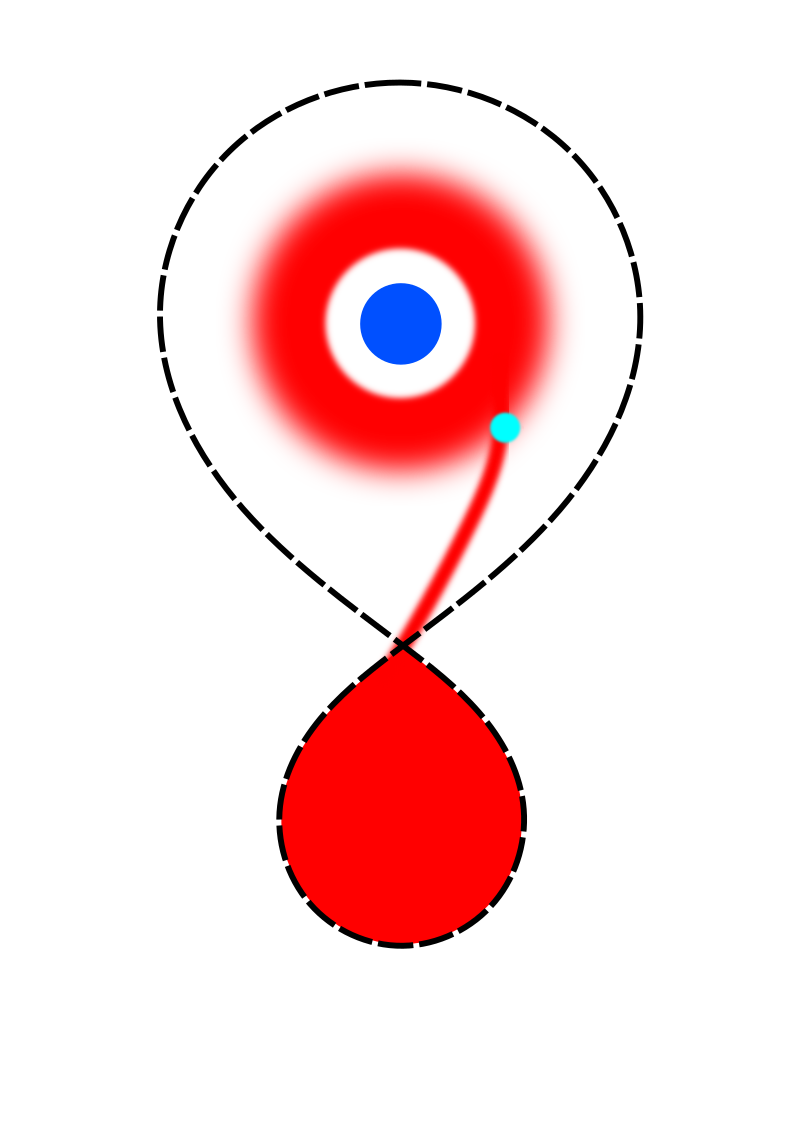
\includegraphics[width=0.6\textwidth]{figures/introduction/CV_schematic.png}
    \caption{A schematic of the structure of a CV, not to scale. The {\bf black dashed line} outlines each Roche lobe. The {\bf dark blue circle} is the white dwarf and is surrounded by its accretion disc. The {\bf lower red teardrop} is the secondary star, and is connected to the donor via the mass stream. The {\bf light blue spot} where the mass stream meets the disc is the bright spot impact region.}
    \label{fig:introduction:CV schematic}
\end{figure}

Systems actively undergoing mass transfer are important to our understanding of stellar evolution. A diversity of stars will experience a mass transfer phase, and losing mass strongly influences a stars' evolutionary path and must be accounted for (e.g. \citealt{renzini1981, smith2014} for single stars, or \citealt{hurley2002} for binaries). Of such systems, CVs in particular are interesting as modelling their eclipse light curves can yield precise, independant measures of both stars' mass and radius \citep{wood1986,Littlefair2008,Savoury2011}. Further, since the donor stars' evolution is dominated by its mass loss, CVs provide a window into binary evolution \citep{knigge2006}.
The mass loss itself is driven by poorly-understood mechanisms, classically attributed to stellar magnetism and gravitational waves, that can also be probed using CV observation and modelling.

Since CVs are binary stars, in the case of eclipsing systems it is possible to make direct observations of orbital separations, stellar masses, and radii. This lends some powerful diagnostics, in addition to parameters accessible with more general techniques such as spectroscopic analysis.
The ability to thoroughly characterise CVs makes them an excellent test-bed for binary modelling, and the complex processes that contribute to their evolution.
Unfortunately, whilst reasonably accurate semi-empirical modelling of most of the CV evolutionary track and population distribution have been now possible for more than a decade (e.g. \citealt{knigge11,Paxton_2015}), the field has yet to produce physically motivated theoretical models capable of accurately reproducing either the CV population distribution or complete evolutionary track, indicating some shortfalls in our understanding \citep{schreiber2015,Schreiber2016}.
Of most significance to this work is the problem of missing Angular Momentum Loss (AML), where CVs with low mass donor stars appear to be losing angular momentum much faster than our models predict \citep{Schreiber2016}. This first chapter will summarise the current understanding of CV formation and evolution, and will focus on the issues with CV evolutionary models.


\section{Roche geometry}
\label{sect:introduction:Roche geometry}

Before discussing the formation, structure, and evolution of CVs, it is first critical to understand Roche lobes.
In a two-body orbital system, the Roche potential of a point is an effective potential in the non-inertial, co-rotating frame of reference. It is given by the sum of the gravitational potential energies due to the two masses, and the potential energy arising from centrifugal force. This can be described mathematically for each position vector:
\begin{equation}
    {\bf \phi} = -\frac{G M_1}{|{\bf r - r}_1|} - \frac{G M_2}{|{\bf r - r}_2|} - \frac{1}{2}({\bf \Omega} \times {\bf r})^2
\end{equation}
Where $\phi$ is the Roche potential, G is the gravitational constant, $\bf r$ is the position vector being considered relative to the centre of mass, and $\bf \Omega$ is the angular momentum vector of the binary. $M_{1,2}$ and ${\bf r}_{1,2}$ are the masses and position vectors of the two orbiting bodies. measured from the centre of mass. Figure~\ref{fig:roche} shows this graphically.
\begin{figure}
    \centering
    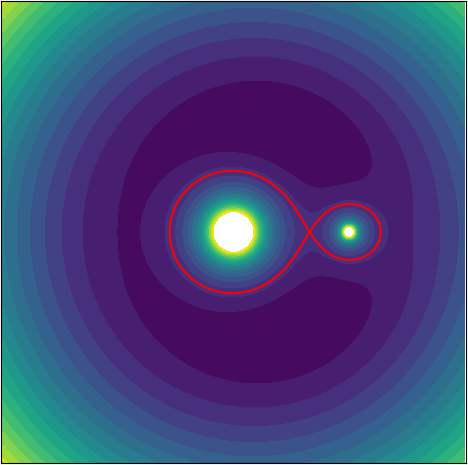
\includegraphics[width=.6\columnwidth]{figures/introduction/roche.png}
    \caption{Showing the Roche potential in the neighbourhood of the binary system, with the more massive primary star on the left. Darker regions are lower potentials, lighter regions are higher potentials. The {\bf red line} illustrates the Roche lobes.}
    \label{fig:roche}
\end{figure}

There are five key locations in the Roche potential, called Lagrange points. The first Lagrange point, $L_1$, is the point at which a small (co-rotating) mass is attracted equally and oppositely by both bodies
We can trace the line of constant potential that passes through $L_1$ giving two teardrops joined at the tips. The teardrop encapsulating an object is known as its Roche lobe.
Matter that lies beyond the Roche lobe is no longer gravitationally bound to that body, and will either fall onto its companion, or leave the surface of the object.
Ejected material will no longer be in a stable orbit, and will go on to either be ejected from the system entirely, or find a new higher orbit where the two-body effects are negligible.

The shape of the Roche lobes are non-trivial to calculate, and must be done numerically. However, approximations exist for the volume-equivalent radius of a Roche lobe (that is, the radius of a sphere of equivalent volume). Most commonly used is the \citet{Eggleton1983} approximation,
\begin{equation}
    \label{eqn:introduction:eggleton approximation}
    \frac{R_L}{a} = \frac{0.49 q^{2/3}}{0.6 q^{2/3} + \mathrm{ln}(1 + q^{1/3})}
\end{equation}
where $a$ is the orbital separation, and $q$ is the mass ratio of the system, $M_2 / M_1$. This formula is accurate to within $\lesssim 1\%$ for all values of $q$. In CVs, where the secondary star is completely filling its Roche lobe, $R_L$ makes for a good approximation for the secondary stars' radius.


\section{Accretion in CVs}
\label{sect:introduction:accretion}
Accretion physics is important to the appearance and behaviour of a CV. whilst it is summarised here, more in-depth descriptions can be found in \citet{warner1995, hellier2001, ritter2010}.

When the donor star overfills its Roche lobe, matter is ejected from its surface at thermal velocities, $\sim 10 \rm km\ s^{-1}$ for a 5000K M dwarf, which is small compared to the orbital velocity of the system (M dwarf velocities of $\sim 400-500 \rm\ km s^{-1}$ are common in the observations reported in Chapters \ref{chpt:results:three peculiar white dwarfs} and \ref{chpt:results:characterisation of 12 new CVs}). Since the ejected material is effectively stationary as it leaves the donor, it falls along a ballistic trajectory towards the white dwarf primary and forms an accretion disc around it.

Disc material gradually loses angular momentum and gravitational potential energy due to its viscosity, which acts over time to concentrate the majority of the disc's angular momentum in the minority of the disc's mass, ejecting some material at high velocities at the expense of moving the remainder closer to the white dwarf.
This viscosity partially arises from friction within the fluid of the disc but the main source is thought to be from turbulence -- random eddy currents moving material to different radii.
This form of turbulence in a thin disc was formalised in the alpha disc model by \citet{shakura1973}, where viscosity, $\nu$, is related to scale height, $H$, and the speed of sound, $c_s$, by a free parameter, $\alpha$.
\begin{equation}
    \label{eqn:disc viscocity}
    \nu = \alpha c_s H
\end{equation}
Since turbulent eddies cannot be larger than $H$ or have velocities greater than $c_s$, $c_s H$ forms the upper limit of $\nu$, and $\alpha$ is limited in this model to values between 0 and 1. In typical CV accretion discs (i.e. quiescent discs, see \S\ref{sect:introduction:dwarf novae}), $\alpha$ takes values from $\sim 0.01 - 0.05$ \citep{hellier2001}.

Material that enters the disc must lose gravitational potential energy before it can be accreted to the white dwarf surface. Approximately half of this energy is lost thermally, through radiating accretion light, and the other half is converted to the kinetic energy necessary to maintain orbit about the white dwarf at lower altitudes. This low orbit has typical velocities roughly an order of magnitude higher than the rotational velocity of the white dwarf, so for material to settle on the stars' surface it must dissipate a large amount of kinetic energy. A region between the inner edge of the disc, and the surface of the white dwarf where this deceleration occurs is called the boundary layer, and can be a significant contributor to the total brightness of a CV.

As the white dwarf is accreting material onto its surface, one might expect it to grow in mass over time, and possibly even detonate as a type Ia supernova when it crosses the $1.4 M_\odot$ Chandrasekhar limit. This postulation is supported by the white dwarfs in CVs being significantly more massive than their singleton counterparts \citep{zorotovic2011}, but were this the case we would expect there to be a relationship between age, and white dwarf mass. \citet{McAllister2019} searched for this relationship, but found no correlation between the two, indicating that the white dwarfs in CVs do not grow over time, and are unlikely to reach the Chandrasekhar limit. Growth is thought to be limited by the accreted material cyclically detonating, in events called Classical Novae outlined in \S\ref{sect:introduction:classical novae} \citep{Wijnen2015,sparks2021}. Serial detonation is even invoked as a potential source of AML, dubbed Consequential AML (CAML), that is described in \S\ref{sect:introduction:CAML}.


\newpage
\section{CV variability and subtypes}
\label{sect:introduction:CV subtypes}
Several subtypes of CV exist that can lie significantly outside the normal evolutionary tracks we expect, contain exotic components, or undergo outbursts.
In addition, it is common for CVs to display a significant short term, stochastic variability, known as flickering. This quasi-random noise is not fully understood, but is known to be localised to the vicinity of the white dwarf \citep{horne1985,bruch1996,bruch2000}, though does not appear to lie directly on it.
Here I briefly describe the various subtypes of CVs, though note that only quiescent CVs are suitable for analysis in this work.

\subsection{Brown dwarf donors}
\label{sect:introduction:brown dwarf donors}

The formation channel of CVs does not require that the secondary star meets any minimum mass requirement, and it is theoretically possible to form a CV with a substellar brown dwarf donor \citep{politano2002,politano2004}. Because the donor is so small, these systems can form well below the theoretical minimum period (see \S\ref{sect:introduction:period minimum and bouncers}), between 46 minutes and 2.5 hours \citep{politano2004}. CVs are observed with extremely short orbital periods, but observational evidence of these hosting brown dwarfs is rare. However, some tentative candidates do exist, for example in SDSS J150722.30+523039.8 (initially \citealt{littlefair2007}, though contested by \citealt{uthas2011})

\subsection{Magnetic CVs}
\label{sect:introduction:magnetic CVs}

It is possible for white dwarfs to have very strong magnetic fields, in the region of tens to hundreds of megaGauss. Such white dwarfs are called polars and are an interesting field of study in their own right, but when a polar is accreting material from a donor star the system is designated as an AM Her star and the intense magnetic field strength alters the CV in a two main ways. The strong field lines of the polar mean that the hot, charged photosphere material transferred to the primary cannot form an accretion disc and instead falls directly onto the surface of the white dwarf. The impacting material forms a bright spot on the white dwarf surface, which is usually bright enough to be visible from earth. In addition, the strong field lines force the white dwarf to become tidally locked to the donor star.

There is also a subclass of magnetic CVs with weaker field strengths of a few megagauss, known as DQ Her stars. In these systems, the white dwarf is not tidally locked, and a partial disc can exist.

\subsection{Helium-rich CVs}
\label{sect:introduction:AM CVn}

A small number of CV donors are helium-rich, with much smaller radii than their hydrogen-rich counterparts; these can be semi-degenerate helium stars, the cores of highly evolved main sequence stars, or a second white dwarf.
As a CV donor must be in contact with its Roche lobe, such systems are far more compact than usual, with orbital periods $\lesssim 65$ minutes. Such systems are AM CVn stars, after the prototypical system AM Canum Venaticorum. For further discussion on AM CVn stars, see \citep{solheim2010}.


\subsection{Classical Novae}
\label{sect:introduction:classical novae}

The white dwarf in a CV is almost constantly accreting matter onto its surface. Over time this surface layer can build up, and is placed under immense pressure by the gravity of the white dwarf. Eventually, pressures rise enough to force material at the boundary to become degenerate, and once hot enough this boundary layer can begin nuclear fusion.
Since the accreted material has become degenerate by this point, it cannot expand in response to the energy injected by fusion and simply heats further, leading to more and more fusion and culminating in a complete detonation of the accreted material on the white dwarf's surface \citep{warner1995}. This detonation heats the material enough to lift degeneracy, and the accreted material is blown from the surface.
These are recognised by a significant brightening of the system of between 6 and 19 magnitudes, lasting anywhere from a few days, to several months.

Once a system has experienced a classical nova, it is classified as a CNe system. \citep{warner1995}. However, theory suggests that all CVs experience classical novae many times over their lifetimes. The required amount of accreted material for the nova to occur depends on the white dwarf mass, but lies between $3\times10^{-5} M_\odot$ of hydrogen for a $1.3 M_\odot$ white dwarf, and $5\times10^{-3} M_\odot$ for a $0.6 M_\odot$ white dwarf \citep{hellier2001}. Typical CV accretion rates are around $10^{-9} M_\odot\ yr^{-1}$ for long period systems, and $10^{-10} M_\odot\ yr^{-1}$ for short period systems \citep{hellier2001, Pala2021}, suggesting classical novae recur every few million years, or every few tens of thousands of years at most.

The amount of material retained by the white dwarf is likely negligible. Both population synthesis \citep{Wijnen2015} and observations \citep{mcallister2017} indicate no evidence of mass growth over time for the white dwarfs in CVs, and hence that the expulsion of the accreted material in a classical nova is complete.

A final note is that some CVs show multiple classical novae in relatively quick succession \citep{schaeffer2010}. These Recurrent Novae (RNe) are distinguished by having more than one observed nova event recorded. As good quality data only exist for the last few centuries, this enforces a soft limit on recurrence interval of a few hundred years, though recent efforts have been made to search ancient records for candidate events \citep{hoffmann2022}. Only a handful of confirmed RNe are known; the variable star index \citep{Watson2006} only contains 12 systems classified as RNe.

\subsection{Dwarf Novae}
\label{sect:introduction:dwarf novae}

CVs also undergo less extreme brightening events, called dwarf nova outbursts. These brighten the system by between 2 and 5 magnitudes \citep{warner1995} and are more brief than typical CNe, lasting less than $\sim 20$ days. However, in contrast to CNe, they have recurrence times much more in line with human timescales, ranging from a few days to some decades. This is due to the fundamental difference in the physical origin of the two phenomena.
Dwarf nova outbursts do not originate directly from either star in the system, but rather from the accretion disc around the white dwarf. Such outbursts are well-described by the disc instability model \citep{cannizzo1993, dubus2018}.

Initially, the disc is in a cooler, ``low'' state with low temperature, low surface density, and low viscosity. Material in the disc moves inwards due to friction from turbulence (see \S\ref{sect:introduction:accretion}) which is relatively weak in the low viscosity material, so radial movement of disc material is slow.

If the accretion rate of donor material exceeds the rate material falls onto the surface of the white dwarf, then a build-up of matter begins in the disc, raising the density and temperature. Eventually, this annulus reaches $\sim 7000K$, at which point hydrogen becomes partially ionised and a rapid further increase in temperature is triggered as the material becomes optically thick and heat is trapped in the disc. In addition, as the temperature and density rise, so does $c_s$, and following Equation~\ref{eqn:disc viscocity}, so does viscosity, even assuming constant $\alpha$. In fact, $\alpha$ {\it rises} during outburst, to $\alpha \sim 0.1 - 0.5$ \citep{hellier2001}. This hot, luminous, ``high'' state is again stable, and the disc is said to be in outburst.

Now that the disc is more viscous, material is moved inwards more readily. The infall rate onto the white dwarf is much increased, and is now higher than the mass transfer rate, so the disc is drained onto the surface of the white dwarf. As it does so, the surface density and temperature begin to fall, and eventually protons and electrons recombine into hydrogen. Recombination is an exothermic process, but the release of energy is outweighed by the material once again becoming optically thin and allowing radiation to more easily escape the disc. The disc now quickly cools back down to the quiescent, ``low'' state, returning to a low surface density, and the cycle can repeat itself. For a more in-depth look at this model, refer to discussions by \citet{cannizzo1993}, \citet{osaki1996},, and \citet{Hameury2002}.

Three types of dwarf novae exist, which exhibit somewhat different behaviour than what is outlined above. The first of which are SS Cyg stars, distinguished by very consistent amplitudes across outbursts, though there is variation in length, shape, and recurrence time.

Z Cam stars exhibit standstills, events where the system enters outburst, peaks in brightness, then begins to dim. However, rather than returning to its quiescent magnitude, the brightness is maintained $\sim 1-1.5$ magnitudes below peak brightness for a long period of time, typically between a few days, and a few years \citep{simonsen2014}.

The third subtype are SU UMa stars. These systems are known for their more complex behaviour, exhibiting superoutbursts and superhumping, and are described in \S\ref{sect:introduction:SU UMa}

\subsection{SU UMa stars}
\label{sect:introduction:SU UMa}

SU UMa stars are distinguished by exhibiting superoutbursts, similar to the regular dwarf nova outbursts that the star still undergoes, but with greater amplitudes and durations, and longer recurrence times. These outbursts are triggered by the disc radius growing to such an extent that it becomes tidally perturbed by the donor star, and becomes elliptical. This can only take place when the donor star is less than $\sim 1/3$ the white dwarf mass, so only short period systems see these superoutbursts. \citep{hellier2001}.
SU UMa stars are known for their superhumps, which also arises from the disc eccentricity. The tidal interaction between the disc and the donor produces an area of increased luminosity at the edge of the disc between the white dwarf and the donor \citep{warner1988}. As the disc is elliptical, the distance between this disc edge and the donor varies over the course of an orbit, causing variation in brightness as the donor moves around the disc.
These fluctuations are the superhumps, and are useful as they provide a diagnostic to the mass ratio for the system as the  \citep{Patterson1998, Patterson2001, patterson2005}.

Because of the strong influence of the donor, the disc is subject to precession, with a precession rate slightly longer than the orbital period. The superhump period, $P_{\rm hump}$ is then a combination of the orbital period, $P_{\rm orb}$, and the precessional period $P_{\rm pr}$,
\begin{equation}
    \frac{1}{P_{\rm hump}} = \frac{1}{P_{\rm orb}} - \frac{1}{P_{\rm pr}}
\end{equation}
and whilst $P_{\rm pr}$ is difficult to observe, both $P_{\rm orb}$ and $P_{\rm hump}$ can be readily observed with photometry. Since the precession period is dependant on the mass ratio and the disc radius, by finding the superhump period of eclipsing CVs an empirical relationship can be found between the superhump excess, $\epsilon$, and the mass ratio of a CV, where:
\begin{equation}
    \epsilon = \frac{P_{\rm hump} - P_{\rm orb}}{P_{\rm orb}}
\end{equation}
and several papers exist discussing and calibrating this relationship, see \citet{McAllister2019} and \citet{kato2022} for some recent calibrations and a good starting point for more information.


\subsection{Novalike systems}

The disc instability model applies to CVs with mass transfer rates that are high enough to exceed the infall rate onto the CV during the ``low'' state, but low enough that the ``high'' state can drive a net loss of mass from the disc. However, a subset of CVs have mass transfer rates high enough to sustain the high state and maintain a permanent outburst mode. Such systems are called novalikes.

Most novalike CVs show little variation besides the stochastic flickering seen in most CVs, though a small number known as VY Scl stars do occasionally enter ``low'' states and dip in brightness by several magnitudes. \citet{livio1994} propose that this is triggered by a starspot rotating into the L1 point causing a fall in mass transfer rate. This fall is because the stellar surface in a starspot is lower than at the unspotted surface, causing the donor to temporarily disconnect from the L1 point whilst the L1 is covered with a spot.
A competing theory from \citet{wu1995} proposes that the fall in brightness is caused by the irradiation of the donor stars' atmosphere driving mass transfer, and that when this irradiation becomes blocked in some way, the mass transfer rate falls enough for the disc to enter the low state for a short time.


\section{CV formation}
\label{sect:introduction:formation of CVs}

The formation of a CV begins with a binary system forming at a distance of $\sim 100{R_\odot}$. Crucially, the stars differ significantly in mass, one typically being $<1{M_\odot}$ and the other $>1{M_\odot}$ \citep{Ritter2012}. The lifespan of a star falls as its mass increases, so the larger star evolves faster than its companion, increasing in radius as it does so. Eventually, the primary fills its Roche lobe, usually when it ascends to the red giant branch.
Once the outer layers of the primary contact the Roche lobe, the $\mathrm L_1$\ point forms a locus for mass to move from the massive, evolved star onto the less evolved secondary star.

As mass moves away from the primary, and away from the centre of mass of the system, it gains angular momentum. However, because angular momentum is conserved within the binary this is offset by a drop in separation, $a$, and the radius of the Roche Lobe, ${R_L}$, contracts following Equation~\ref{eqn:introduction:eggleton approximation}. \textit{More} matter is now outside the primary Roche lobe, encouraging further mass transfer and hence further reduction in orbital separation \citep{Ritter2008}.

With this positive feedback loop, the primary can quickly transfer its whole envelope. The process is very rapid -- so rapid that models have been unable to properly resolve it, but is probably $\sim 10^2 - 10^3$ years in duration \citep{Ritter2012}. With this influx of mass, the secondary star grows and the accreted matter forms a thick, bloated, deeply convective envelope on the star. The increased radius of the secondary brings the two bodies into contact \citep{Ritter2008} and the stars enter a common envelope phase of evolution. See \citet{paczynski1976} for an original reference on common envelope evolution, or \citet{ivanova2020} for a recent review of the topic. For detail on this phase as it relates to CVs, see \citet{taam1978, webbink1984, zorotovic2010, passy2011}.

The common envelope phase transfers much of the secondary stars' angular momentum to the shared envelope, though the mechanism for this is poorly understood \citep{demarco2011}.
If the common envelope is substantial enough, all the energy can be removed from the orbit and the two stars will merge.
If it is not substantial enough, the entire common envelope is unbound from the stars before a merger occurs, and the stars are left in a more compact orbit than when the common envelope phase began.
CV systems are the product of the latter scenario - the common envelope is ejected via a strong wind, leaving the remnant core of the primary as a white dwarf, and a low mass secondary companion M dwarf still on the main sequence.

The common envelope phase can be parametrised with the energies involved, namely the gravitational binding energy of the envelope, $U_{\rm bind}$, and the change in the angular momentum contained in the orbit before and after the common envelope phase, $\Delta U_{\rm orb}$, as the common envelope efficiency parameter, $\alpha$.
\begin{equation}
    \alpha = \frac{U_{\rm bind}}{\Delta U_{\rm orb}}
\end{equation}
This is known as the $\alpha$ formalism \citep{demarco2011}, and is a good illustration of how poorly we understand CE evolution. $\alpha$ should be a metric we can predict with models, but this has proven very challenging and several competing frameworks exist \citep{ivanova2020}.

The energy needed to liberate the envelope is expected to come from the orbit of the binary, but some systems have been observed and characterised with $\alpha > 1$. suggesting that other sources, like the thermal output of the stars, can contribute to the envelope ejection \citep{demarco2011, ivanova2013}. Common envelope evolution remains a very difficult problem to solve, and only approximate models currently exist \citep{ivanova2020}, but the following scenario is generally accepted as likely in the case of CVs.

For proto-CVs, $\alpha$ has been loosely estimated to be $\sim 0.2 - 0.6$ \citep{politano2007}, and some evidence exists for lower $q$ systems having larger $\alpha$ \citep{passy2013}. The ejecta carries with it angular momentum, causing $a$ to quickly fall from $\sim 100 R_\odot$ to a few $R_\odot$ \citep{politano2007}.
Following the common-envelope phase, angular momentum is shed through magnetic braking and gravitational wave braking until the donor comes into contact with its Roche lobe, a process that takes $\sim 1-2$ Gyrs. Mass transfer can then resume, though this time in the more stable secondary-to-primary direction. The system is now a CV, and its evolution from here will be dominated by AML and mass transfer, detailed in \S\ref{sect:introduction:AMLMechs}.

Early population studies expect that under this formation process up to 50\% of CVs should host a helium white dwarf \citep{politano1996}, though to date this has been difficult to test.
\citet{zorotovic2010} examined a sample of post-common envelope binaries and found only $13\pm7\%$ of the sample to be expected to evolve into a CV containing a helium white dwarf. However, no confirmed helium white dwarfs have been observed in CVs.


\section{CV evolution}
\label{sect:introduction:Summary of how AML and Mdot drive period evolution}

Initially, mass from the more massive star transferred to the smaller one, but once the system emerges from the common envelope phase, AML causes the orbit to tighten until the less massive red dwarf secondary fills its Roche lobe. Converse to during formation, mass transfer is now moving matter closer to the system's centre of mass, imparting angular momentum to the secondary as it does so. This causes the orbit to widen, and increases $R_L$. Hence, mass transfer now acts to decrease further transfer \citep{Ritter2008}, rather than exacerbate it.

To maintain mass transfer some mechanism is necessary to shed angular momentum and bring the secondary back in contact with its Roche lobe.
Canonically, two mechanisms are thought to drive this; gravitational wave braking, and magnetic braking \citep{knigge2006,knigge11}.
AML drives the two bodies closer together and triggers mass transfer, and mass loss from the donor drives it to retreat from the white dwarf primary. These two processes find equilibrium when the donor is just barely overflowing its Roche lobe, and the angular momentum gained by the donor from mass transfer is offset by the AML from the system.
The mass transfer timescale of the donor is much shorter than its nuclear timescale, so mass loss dominates its evolution and gives rise to a single, unified CV evolutionary path.

There is a further complicating factor to consider; whilst the secondary is losing mass, it is not in thermodynamic equilibrium. The outer layers are being lost, which reduces the pressure on the core and so reduces the rate of fusion.
Above masses of $\sim 0.1 M_\odot$, the thermal timescale is much longer than the mass loss timescale (this is later demonstrated in \S\ref{sect:modelling:evolutionary modelling}), so the star is unable to cool and contract to its equilibrium radius. This leaves the star hotter than it would be under zero mass loss, and its radius increased proportionally to the mass loss rate \citep{knigge2006, knigge11}.


\subsection{The classical picture of CV evolution}
\label{sect:introduction:AMLMechs}

When two bodies orbit each other in space, the periodic warping of space-time produces gravitational waves \citep{einstein1918} and these waves carry energy away from the system, robbing it of angular momentum and reducing the orbital radius \citep{Paczynski1967}. In CVs, the rate of momentum loss from gravitational waves is small, so long timescales are needed to significantly alter the orbital period.
Both population synthesis models and evolutionary models of CVs do not match the observed population distribution with gravitational braking alone, and magnetic braking is thought to make up the deficit (e.g. \citet{kolb1993a, kolb1993, Davis2008, garraffo2018b}).
A quantitative description of the some magnetic braking models are given in \S\ref{sect:introduction:magnetic braking}. Before discussing the braking mechanisms in CVs, it is important to review the classical understanding of CV evolution


\subsection{The effect of mass transfer on the binary}
\label{sect:introduction:stability criterion}


When mass moves from the donor to the white dwarf primary, the redistribution of matter within the system must take place whilst conserving angular momentum. The total angular momentum of the binary, $J$, is given by,
\begin{equation}
    J = M_1 a_1 v_1 + M_2 a_2 v_2 = M_1 a_1 \frac{2\pi a_1}{P_{orb}} + M_2 a_2 \frac{2\pi a_2}{P_{orb}}
\end{equation}
where the distance from each star to the centre of mass is $a_{1,2}$, and the velocity of each star is $v_{1,2}$.
The binary separation between the stars is $a = a_1 + a_1$, and the ratio between the stars' distances to the centre of mass is the inverse of their mass ratio, i.e. $\frac{a_2}{a_1} = \frac{M_1}{M_2}$. By substituting $P_{orb}$ for Kepler's 3rd law, we can construct a simple equation for $J$,
\begin{equation}
    J = M_1 M_2 \bigg( \frac{Ga}{M_1 + M_2} \bigg)^{1/2}
\end{equation}
Now, by taking the natural log of both sides and differentiating with respect to time we find the following relation between the derivatives.
\begin{equation}
    \frac{\dot a}{a} = 2\frac{\dot J}{J} + \frac{(\dot M_1+\dot M_2)}{M_1+M_2} + 2\frac{\dot M_1}{M_1} + 2\frac{\dot M_2}{M_2}
\end{equation}
For the specific case where the total system mass is fully conserved, we can use $\dot M = 0$, $\dot M_1 = -\dot M_2$, and $\dot J \equiv 0$ to simplify the above
\begin{equation}
    \label{eqn:introduction:orbital separation change due to mass transfer}
    \frac{\dot a}{a} = 2\frac{\dot M_1}{M_1} + 2\frac{\dot M_2}{M_2} = 2(q-1) \frac{\dot M_2}{M_2}
\end{equation}
or by similarly differentiating the logarithm of $P_{orb}^2 \propto a^3$,
\begin{equation}
    \label{eqn:introduction:orbital period change due to mass transfer}
    \frac{\dot P_{orb}}{P_{orb}} = \frac{3}{2}\frac{\dot a}{a} = 3(q-1) \frac{\dot M_2}{M_2}
\end{equation}

Equations \ref{eqn:introduction:orbital separation change due to mass transfer} and \ref{eqn:introduction:orbital period change due to mass transfer} tell us how the binary responds to mass transfer. As mass is lost from the secondary, $\dot M_2$ is negative and we can see that systems with $q>1$ will have their orbits contract, and systems with $q<1$ will have their orbits widen in response to mass transfer.

We must also consider the response of the Roche lobe radius to mass transfer.
A simpler, more easily manipulated alternative to the Eggleton $R_L$ approximation (Equation~\ref{eqn:introduction:eggleton approximation}) from \citep{paczynski1971},
\begin{equation}
    \frac{R_L}{a} = 0.462 \frac{q}{1 + q}^{1/3}
\end{equation}
although this only holds between $0 < q < 0.8$ and is accurate to 2\%. Taking the logarithm, differentiating with respect to time, and substituting Equation~\ref{eqn:introduction:orbital separation change due to mass transfer},
\begin{equation}
    \label{eqn:introduction:Roche lobe in response to mass loss}
    \frac{\dot R_L}{R_L} = \frac{\dot a}{a} + \frac{\dot M_2}{3 M_2} = \bigg ( 2q - \frac{5}{3} \bigg )\frac{\dot M_2}{M_2}
\end{equation}
However, this reveals the flaw in assuming fully conservative mass transfer ($\dot M \equiv 0$, $\dot J \equiv 0$) and using the simpler $R_L$ approximation, as this implies that for $q < 5/6$, $R_L$ will increase in response to mass transfer. This is not compatible with continuous mass transfer without some mechanism (such as the nuclear expansion of an evolved donor ascending the red giant branch, as during the CV formation), and as most CVs are observed with $q < 5/6$ and do not possess such a mechanism.

Finally, we can also approximate the stability criteria for mass transfer using the equations above.
The maximum stable value of $q$ can be found by considering the mass-radius exponent of the donor ($\xi$), and its Roche lobe ($\xi_{\rm L}$). For the donor, $\xi$ can be found by simply differentiating the general equation $R \propto M^\xi$.
\begin{equation}
    \xi = \frac{{\rm d\ ln\ }R_2}{{\rm d\ ln\ }M_2}
\end{equation}
Similarly, by using Equation~\ref{eqn:introduction:Roche lobe in response to mass loss} we find
\begin{equation}
    \xi_{\rm L} = \frac{{\rm d\ ln\ }R_L}{{\rm d\ ln\ }M_2} = 2q - \frac{5}{3}
\end{equation}

For stable mass transfer, the response of the Roche lobe must be less than the response of the donor, $\xi > \xi_{\rm L}$. This ensures that mass loss causes the star to contract more than the Roche lobe contracts, and gives the following stability criterion,
\begin{equation}
    q < \frac{1}{2}\xi + \frac{5}{6}
\end{equation}
for which we can substitute in a theoretical value of $\xi$ to find the maximum $q$. For a low mass, main sequence star ($M < 0.8M_\odot$), $\xi \simeq 0.8$ \citep{knigge11} and we find $q < 1.23$. Below $M_2 \lesssim 0.43 M_\odot$, the star becomes deeply convective and $\xi$ falls sharply to $\xi = -1/3$ \citep{paczynski1965,rappaport1982}, and $q \lesssim 2/3$.


\subsection{Period evolution and key population features}
\label{sect:introduction:period distribution key features}
\begin{figure}
    \centering
    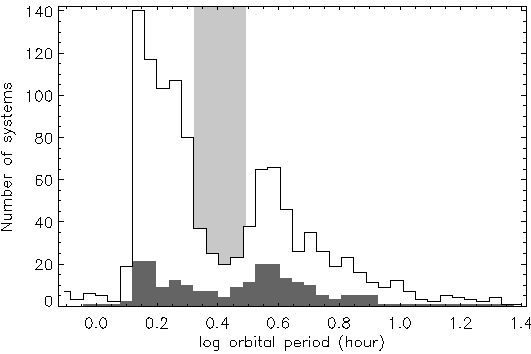
\includegraphics[width=\columnwidth]{figures/introduction/pd-rk.pdf}
    \caption{Reproduced from \citet{southworth2015}, Figure~14. The orbital period distribution of RKCat \citep{RKCat} CVs identified by the SDSS ({\bf white histogram}) and of the subset of these which are eclipsing ({\bf grey histogram}). The {\bf light grey shaded region} illustrates the period gap at 2.1 - 3.1 hours. The periods have been collected into histogram bins which are of equal size in log space.}
    \label{fig:period hist}
\end{figure}

The orbital period of a CV can be measured by tracking either their spectroscopic radial velocities (e.g. \citealt{gaensicke2009}), or the timings of repeating features in their light curves (e.g. \citealt{Littlefair2008}). Once this has been done for a large enough sample \citep{southworth2015}, a histogram of the periods can be plotted. This plot, shown in fig.~\ref{fig:period hist}, has three immediately obvious features:
\begin{itemize}
    \item a long period cutoff, as the number of systems taper off after $\sim12$hrs
    \item a period gap at $\sim2-3$hrs
    \item a period minimum at $\sim1$ hour, with a pile-up of systems just above it.
\end{itemize}
Each of these features are discussed in turn.

\subsubsection{The period maximum}
\label{sect:introduction:period maximum}
In order for a system be be a CV, mass must be transferring from a less massive star, onto a compact object, constraining the maximum value of $q$ to $\sim1$, and demanding that the secondary extends out to $\sim R_L$.

There are three constraints on a CV pertinent to the maximum allowable period. The mass ratio, $q = \frac{M_{\rm donor}}{M_{\rm wd}}$, must be low enough for thermally stable mass transfer ($q < 1.23$, \S\ref{sect:introduction:stability criterion}, here approximated as $q = 1.0$), the donor radius must be approximately equal to the Roche radius, and maximum mass of a white dwarf is well known to be limited to $\le 1.4M_{\odot}$ before triggering thermonuclear runaway \citep{chandrasekhar1942}.

Now, to find the theoretical period maximum, we simply find the period corresponding to the largest possible donor star. \citet{warner1995} shows that the average density, $\rho_{av}$, for objects that fill their $R_L$ follows a robust relationship;
\begin{equation}
    \frac{\rho_{av}}{\rho_{\odot}} = 75.9 P_{orb}^{-2}(h)
\end{equation}
\citet{knigge11} derived a connection between CV secondary mass and radius, $M_2$ \& $R_L$. This can be manipulated to produce a mass-period relationship,
\begin{align}
    \rho_{av} = \frac{3 M_2}{4 \pi R_L^3} &\simeq 75.9 P(h)^{-2} \\
    \frac{R_L}{R_\odot} = C &\cdot \Big( \frac{M_2}{D \cdot M_\odot} \Big) ^{\alpha}
\end{align}
where $C$ and $D$ are constants for a particular regime, i.e., short-period, long-period, or period bouncer, and $\alpha$ is the mass-radius index \citep{Knigge2011b}.
Combining the above gives a pleasingly simple relationship.
\begin{equation}
\label{eqn:MP_relation}
    M_2^{(1-3\alpha)} \propto P^{-2}
\end{equation}

For long-period CVs, $\alpha = 0.67\pm0.04$ \citep{knigge11}, and equation \ref{eqn:MP_relation} becomes $M_2^{1.01} \propto P^{2}$, and larger secondary masses require longer periods. The theoretical maximum secondary mass of $1.4 M_{\odot}$ corresponds to a period of $\sim12$hrs, though in reality these higher mass donors are rarer and the frequency of CVs at these higher periods begins to drop much earlier, at $\sim6$hrs \citep{gaensicke2009}.


\subsubsection{The period gap}
\label{sect:introduction:period gap}

Between periods of around 2-3 hours, there is a dramatic fall in the number of CVs we detect and volume-limited samples indicate that this is a real effect and not a selection bias \citep{Kolb1998,pala2020}. The origin of this gap in the period distribution is something of an open problem.

Models indicate that long period systems ($P > 3$h) have far higher mass loss rates than short period systems ($P < 2$h) \citep{ritter1985}. This suggests a significant change in braking mechanisms between the two regimes.
Recall that the donor star is inflated by mass loss (\S\ref{sect:introduction:Summary of how AML and Mdot drive period evolution}).
If the cutoff of angular momentum loss is sharp, i.e. magnetic braking suddenly ceases, the donor is allowed to contract to its equilibrium radius and disconnects from its Roche lobe, shutting off mass transfer.
The system is still subject to gravitational radiation, however, so gradually continues to evolve towards shorter periods. Once the secondary reconnects with its Roche lobe, mass transfer resumes and the system again presents itself as a CV, emerging from the period gap at a $\sim2$hr period \citep{kolb2002}.

The disruption of magnetic braking was proposed early on to explain the period gap \citep{rappaport1983, spruit1983}, and relatively shortly after \citet{kolb1993} showed more quantitatively that a sub-class of purely gravitational braking CV systems does not reproduce the observed population.
The classical evolutionary path of CVs has involved the secondary becoming fully convective which was thought to disrupt the magnetic field and so cease magnetic braking \citep{knigge11}.
\citet{Davis2008} used population synthesis to demonstrate that, if the period gap is caused by disrupted magnetic braking, this may affect the mass function of quiescent CVs that are moving through the gap. They expect an excess of non-transferring CVs over low mass post-common envelope CVs that emerge from the common envelope phase directly into the period gap.
These should form at a predictable rate across $q$, but due to the slow crossing of quiescent CVs the latter `pile up' in the gap - a detectable effect observed by \citet{zorotovic2011}.


\subsubsection{The period minimum, and period bouncer systems}
\label{sect:introduction:period minimum and bouncers}

The period minimum was first predicted by \citet{rappaport1982}, and can be understood by considering the two governing timescales affecting the secondary.
For donors with masses above $\sim0.1 M_{\odot}$, the donor is contracting in response to mass loss.
As this proceeds, both the Kelvin-Helmholtz (a.k.a. thermal) timescale, $\tau_{\rm KH}$, and mass transfer timescale, $\tau_{\dot M}$, are increasing (the latter due to $\dot M_2 / M_2$ rising as the period shrinks). However, $\tau_{\rm KH}$ rises faster, and at a period of $\sim80$ minutes \citep{ritter1998, McAllister2019}, $\tau_{\rm KH}$ exceeds $\tau_{\dot M}$, causing the donor to lose mass adiabatically and expand rather than contract in response to mass loss.
This allows the donor to remain in contact with its Roche Lobe when mass loss raises it to a higher orbit, and the system evolves to longer periods over time.

More quantitatively, as the components of a short period CV move closer together and the donor falls in mass, $\tau_{\rm KH}$ and $\tau_{\dot M}$ become more out of balance, corresponding to $\alpha$ in equation \ref{eqn:MP_relation} decreasing \citep{Knigge2011b}. A main-sequence star will have $\alpha \sim 1$, but a secondary subjected to fast, adiabatic mass loss will have $\alpha \simeq -1/3$. Looking at the gradient of equation \ref{eqn:MP_relation}, the existence of a period minimum can be easily seen.
\begin{equation}
    \frac{\dot P}{P} = \frac{(3\alpha - 1)}{2} \frac{\dot M_2}{M_2}
\end{equation}
When $\alpha \le 1/3$, a negative $\dot M$ will produce a \textit{positive} change in $P$, and the donor begins to retreat from the white dwarf \citep{rezzolla2001}.

This has been confirmed by \citet{knigge11}, who found that for period bouncer CVs, $\alpha = 0.21^{+0.05}_{-0.10}$, giving the following empirical version of equation \ref{eqn:MP_relation} in the post-period minimum regime.
\begin{align}
    M_2 \propto P^{-5.4}
\end{align}


\subsection{Problems with the classical picture}
\label{sect:introduction:modern AML}

A solid knowledge of exactly how and why CVs lose angular momentum has remained surprisingly elusive for several decades now. Early theories established gravitational waves and magnetic braking as the two main sources of AML, but attempts to quantify this with evolutionary models and population synthesis models consistently fall short. Gravitational losses are well understood, and have been independantly observed and studied, but the sources and consequences of magnetic braking is not so easy.

% The spin rates and masses of CV donors are not seen in the singleton stars that are usually used to characterise magnetic braking \citep{rappaport1983,matt2015,garraffo2018a}.
% In addition, the disruption of magnetic braking is often motivated by the donor transitioning to a fully convective state, but X-ray emission level is a diagnostic of magnetic flux \citep{pevtsov2003}, and \citet{wright2016} found that the X-ray flux of main sequence stars is similar between fully convective and non-convective main-sequence stars, implying a similar magnetic field strength. Furthermore, disagreement between observational and theoretical period gap and minimum locations \citep{knigge11} has left the disrupted magnetic braking model an area of active research.
% \citet{garraffo2018b} recently proposed that the magnetic field does not weaken, but rather becomes more complex which reduces the efficiency of magnetic braking. This concept is discussed quantitatively in \S\ref{sect:introduction:Garraffo magnetic braking prescription}.


\subsection{The missing AML problem}
\label{sect:introduction:the missing aml problem}

The evolution of CVs is driven by the donor stars. The orbital period is determined by the mass-radius relationship of the donor under mass loss, and the decay of the orbit should simply result directly from the two braking mechanisms (gravitational and magnetic). Figure~\ref{fig:introduction:Knigge 2011 figure 9} shows the relationship between the donor mass and orbital period, and the single unified CV track can be seen in the observations. CV evolution models can be built to try and reproduce this track, and indeed at long periods, our understanding of those mechanisms seem robust enough to produce models that satisfy observations. The period gap can, with some manual tweaks, also be reproduced with some accuracy. Unfortunately, at short periods ($\lesssim 2$ hours), the data begin to diverge from models \citep{knigge2006,knigge11}.

Section \ref{sect:introduction:Summary of how AML and Mdot drive period evolution} describes how the donor's mass-radius relation is altered by the presence of continued mass loss. The donor is larger than a singleton of the same mass, as the mass loss timescale is comparable to the thermal timescale and the donor is not quite able to maintain thermal equilibrium \citep{knigge11}. The degree of this inflation increases with more rapid mass loss. As mass loss is driven by AML, it follows that a CV donor that has stronger AML will have a larger radius, and therefore sit at a longer period than a CV with weaker AML, altering the gradient of the tracks in Figure~\ref{fig:introduction:Knigge 2011 figure 9} at periods of $\lesssim 3$ hours. In this way, the shape of the tracks in Figure~\ref{fig:introduction:Knigge 2011 figure 9} is a diagnostic of the form of AML experienced by a CV across its lifetime \citep{knigge11}.

\citet{knigge11} used observations of donor masses and radii and attempted to recreate the donor evolutionary sequence.
An unknown additional source of AML was added to their models, simply scaled relative to gravitational braking. This unknown contribution to AML is motivated by the disagreement between data and the model that omits this source. \citet{knigge11} find that the best-fit model to their data uses an excess braking below the period gap that is $2.47 \times \dot J_{GR}$, where $\dot J_{GR}$ is the AML due to gravitational waves. Figure~\ref{fig:introduction:Knigge 2011 figure 9} is reproduced from their work, and shows the significant improvement in agreement with data.
\begin{figure}
    \centering
    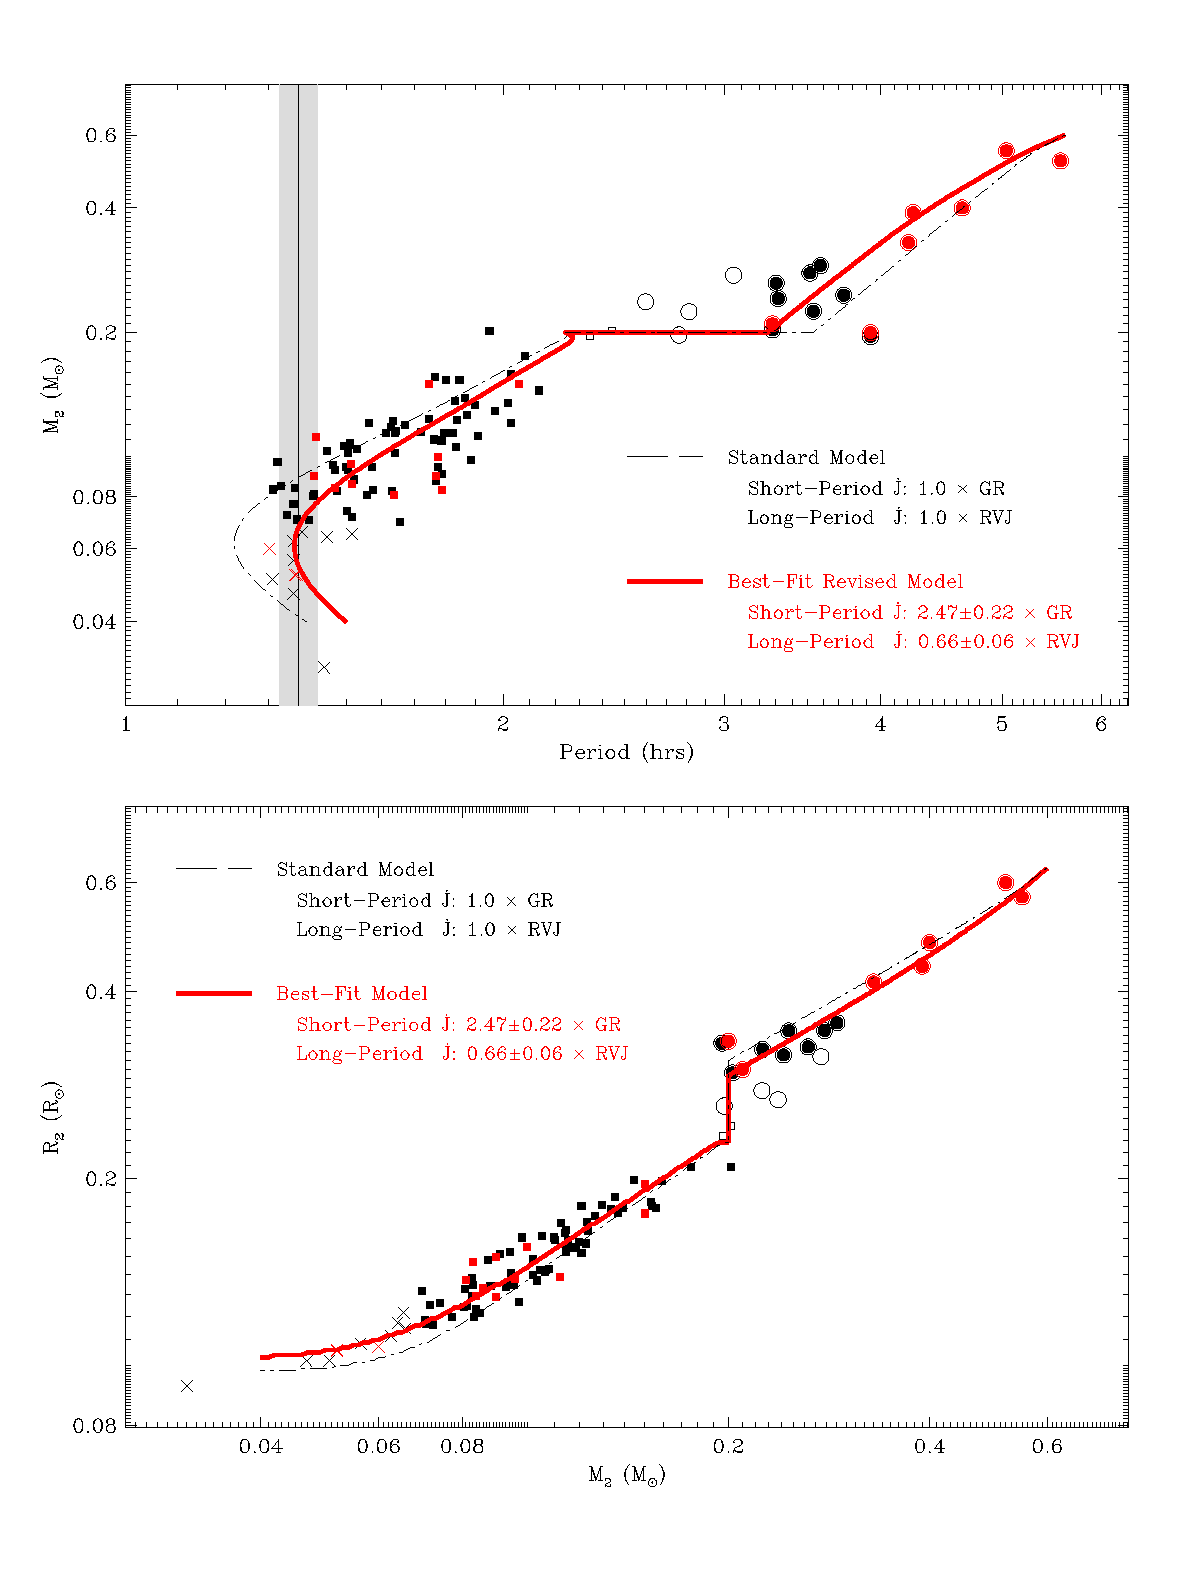
\includegraphics[width=\textwidth, trim={0 2cm 0 2cm}]{figures/introduction/Knigge11_fig9.pdf}
    \caption{Reproduced from \citet{knigge11}. {\bf Black} markers are data from superhumpers, {\bf Red} markers are data from eclipsers. {\bf Crosses} denote candidate period bouncer CVs, {\bf Squares} are short-period CVs, and {\bf Circles} are long period CVs. {\bf Open symbols} are omitted from their analysis due to lying in the period gap. The {\bf Dashed Black lines} are their `standard', na\"ive model, and the {\bf Solid Red line} includes an empirically determined excess AML source, scaled to gravitational wave braking. In the top panel, the {\bf Vertical black line} signifies the observed period minimum, with the grey region as the FWHM of the period spike as measured in \citet{gaensicke2009}.}
    \label{fig:introduction:Knigge 2011 figure 9}
\end{figure}

\citet{Pala2017a} used the effective temperatures of the white dwarfs to probe CV evolution. The white dwarf temperature can be enhanced by accretion, so a hotter white dwarf suggests a higher mass transfer rate. This is sensitive to changes in $\dot M$ on relatively short timescales ($\sim 10^4$ yrs), but still provides a valuable insight. \citet{Pala2017a} compare their white dwarf temperatures (and therefore mass transfer rates, and therefore AML rates) to MESA CV evolutionary tracks, and find that their observed temperatures are poorly described by only gravitational AML, but are more well-fitted by models that includes excess AML equivalent to gravitational losses, i.e. double-strength gravitational AML.

The disagreement between theory and observation at short periods indicates that our understanding of AML in this regime is lacking, and a few proposals to rectify this have been suggested.

The obvious solution to the problem of missing AML is that we simply do not understand magnetic braking well enough to say that it fully disappears below the period gap. The donor may retain a residual magnetic field strong enough to drive some weaker form of magnetic braking that remains after the bulk of magnetic braking ceases, a.k.a. residual magnetic braking.

The period gap is frequently attributed to a fall in magnetic braking when the donor becomes fully convective, due to a large reduction in magnetic field strength. However, observations of field M dwarfs of similar masses, with convective envelopes, are seen with key tracers of magnetism. Specifically, X-ray observations find that the coronal magnetic energy dissipation of fully convective stars is similar to non-convective stars \citep{wright2016}, and Zeeman-Doppler imaging of rapidly rotating M dwarfs indicate that magnetic fields remain strong, whilst the complexity of surface magnetic fields increases alongside rotation rate (e.g. \citealt{donati2003,donati2009,marsden2011,waite2011,waite2015}).
Together, these observations strongly indicate that the disrupted magnetic braking model commonly accepted is ill-motivated, and may be more closely tied to field complexity than field strength \citep{garraffo2018b}. If the gap is indeed driven by a sudden increase in field complexity, then it is reasonable to assume that magnetic braking may remain significant after the system emerges from the period gap.

% Additionally, the whilst magnetic braking is obviously not possible with too weak a magnetic field, it is also not possible under magnetism that is too strong. Some evidence for AML suppression under strong magnetic fields, though not in the context of the period gap, has been found in binary population synthesis models that focus on magnetic CVs \citep{belloni2020}. The models that include magnetic wind suppression under a strong white dwarf magnetic field result in a better fit to key CV observables -- specifically the orbital period distribution, white dwarf temperature distribution, and space density.

Magnetic braking is not the only possible explanation for excess AML, and another strong candidate is consequential AML. This mechanism is discussed below.


\subsection{Consequential AML}
\label{sect:introduction:CAML}

Consequential AML (CAML) is an additional source of momentum loss, originally motivated physically as a second source of magnetic wind emanating from the inner regions of the white dwarf accretion disc \citep{king1995,schenker1998}. In more modern considerations of CAML, the excess loss is explained as nova events temporarily immersing the system in a viscous medium, causing drag on the two bodies and reducing their orbital separation \citep{Schreiber2016}.
In each case, this AML is ``consequential'', in the sense that they rely on either a pre-existing disc to be present or the white dwarf to be accreting enough mass to trigger novae, and the CAML disappears in the absence of existing AML.
By modelling CV evolution including this process, several issues of older CV population synthesis and evolutionary models can be solved at once \citep{Schreiber2016}. These issues are:
\begin{enumerate}
    \item the observed mass of CV white dwarfs is systematically higher than singleton white dwarfs (e.g. \citealt{McAllister2019,pala2020});
    \item since the short period regime has much lower AML rates, CVs should spend most of their time below the period gap, and $\sim 99\%$ of CVs are expected to be short period \citep{kolb1993a}, but observations see a less severe imbalance between long (17\%) and short (83\%) period systems \citep{pala2020};
    % roughly even distribution between long and short period systems \citep{knigge2006};
    \item under purely gravitational losses, the period minimum was first calculated at $\sim 67$ minutes \citep{kolb99}, but is observed at $\sim 79$ minutes \citep{McAllister2019};
    \item the space density of CVs is roughly 1-2 orders of magnitude lower than population synthesis models predict.
\end{enumerate}
The introduction of a modified, empirically calibrated CAML produces models that do not suffer from these issues, making a compelling case for its validity.

The maximum dynamically stable mass transfer rate of a CV is a function of $q$, related via the adiabatic mass-radius exponent, $\xi_{ad}$, and the mass-radius exponent of the Roche radius, $\xi_{L}$. Where the two intersect forms a threshold beyond which runaway mass transfer (much like the pre-CV common envelope phase) is triggered, and most likely results in a merger between the two bodies. We begin similarly to the derivation in \S\ref{sect:introduction:stability criterion},
\begin{equation}
    \label{eqn:introduction:CAML stability threshold}
    \xi_{ad} = \frac{{\rm d} ln(R_2)}{{\rm d} ln(M_2)}_{ad} = \frac{{\rm d} ln(R_L)}{{\rm d} ln(M_2)} = \xi_L
\end{equation}
where $\xi_{ad}$ for convective stars is $-1/3$. Recalling the Eggleton approximation for the Roche radius, Equation~\ref{eqn:introduction:eggleton approximation}, we can find $\xi_{ad}(q)$ \citep{Schreiber2016} in the absence of CAML,
\begin{equation}
    \xi_{ad} = \frac{2}{3}\frac{ln(1+q^{1/3}) - \frac{1}{2}\frac{q^{1/3}}{1+q^{1/3}}}{0.6q^{2/3} + ln(1+q^{1/3})} (1 + q) + 2(q - 1) = -1/3
\end{equation}
Solving this equation gives a critical maximum value of $q \lesssim 0.634$. However, under CAML, extra sources of $\dot J$ are introduced. For example, under the classical non-conservative construction, $\dot J_{CAML}$ is due to nova ejecta carrying angular momentum away from the system as it leaves, contributing
\begin{equation}
    \frac{\dot J_{CAML}}{J} = \nu \frac{\dot M_2}{M_2}
\end{equation}
Here, $\nu = M_2^2 / (M_1(M_1 + M_2))$ and encapsulates the assumption that the angular momentum carried by ejected nova material is equal angular momentum to the white dwarf.
The right hand side of Equation~\ref{eqn:introduction:CAML stability threshold} is then altered by the increased AML rate.
\begin{equation}
    \xi_{ad} = \frac{2}{3} \Bigg( \frac{ln(1+q^{1/3}) - \frac{1}{2}\frac{q^{1/3}}{1+q^{1/3}}}{0.6q^{2/3} + ln(1+q^{1/3})} \Bigg) + 2\nu + \frac{M_2}{M_1 + M_2} - 2
\end{equation}
The effect of this altered form of $\xi_{ad}$ is that CVs with higher mass ratios are stable. Binary population synthesis models by \citet{Schreiber2016} demonstrate that this model is not compatible with observations, producing {\it more} CVs with low mass donors than the non-CAML model and actually performing worse than models that don't include this version of CAML. However, by altering the form of $\nu$ so that it is no longer tied to the white dwarf's angular momentum, a much better agreement with observations can be reached. This is the empirical CAML model, or eCAML.

$\nu$ is altered to a simple function of the white dwarf primary mass,
\begin{equation}
    \label{eqn:introduction:eCAML nu}
    \nu ( M_1 ) = \frac{C}{ M_1 }
\end{equation}
where $C$ is an arbitrary constant chosen to best reflect observations, and \citep{Schreiber2016} adopt values of $C = 0.3 - 0.4$.
The inverse relationship of more CAML at lower white dwarf masses is motivated by lower mass systems ejecting nova material at a lower velocity, meaning the binary is immersed in a friction-generating medium for longer and imparting more energy into the ejecta.

With eCAML, the dynamically unstable region is expanded. This has the important effect of making CVs with low-mass white dwarfs prone to dynamically unstable mass transfer (see \S\ref{sect:introduction:stability criterion}), removing them from the CV population -- this simultaneously answers the question of CV white dwarfs being more massive than expected, and also vastly lowers the space density \citep{belloni2018}. Finally, the majority of systems that are now dynamically unstable are short-period CVs, so the observed period distribution is significantly more well-reproduced. Figure~\ref{fig:introduction:Schreiber 2016 figure 2} is reproduced from \citet{Schreiber2016}, and shows the three dynamically unstable regions graphically.
\begin{figure}
    \centering
    \begin{minipage}[b]{\textwidth}
        \centering
        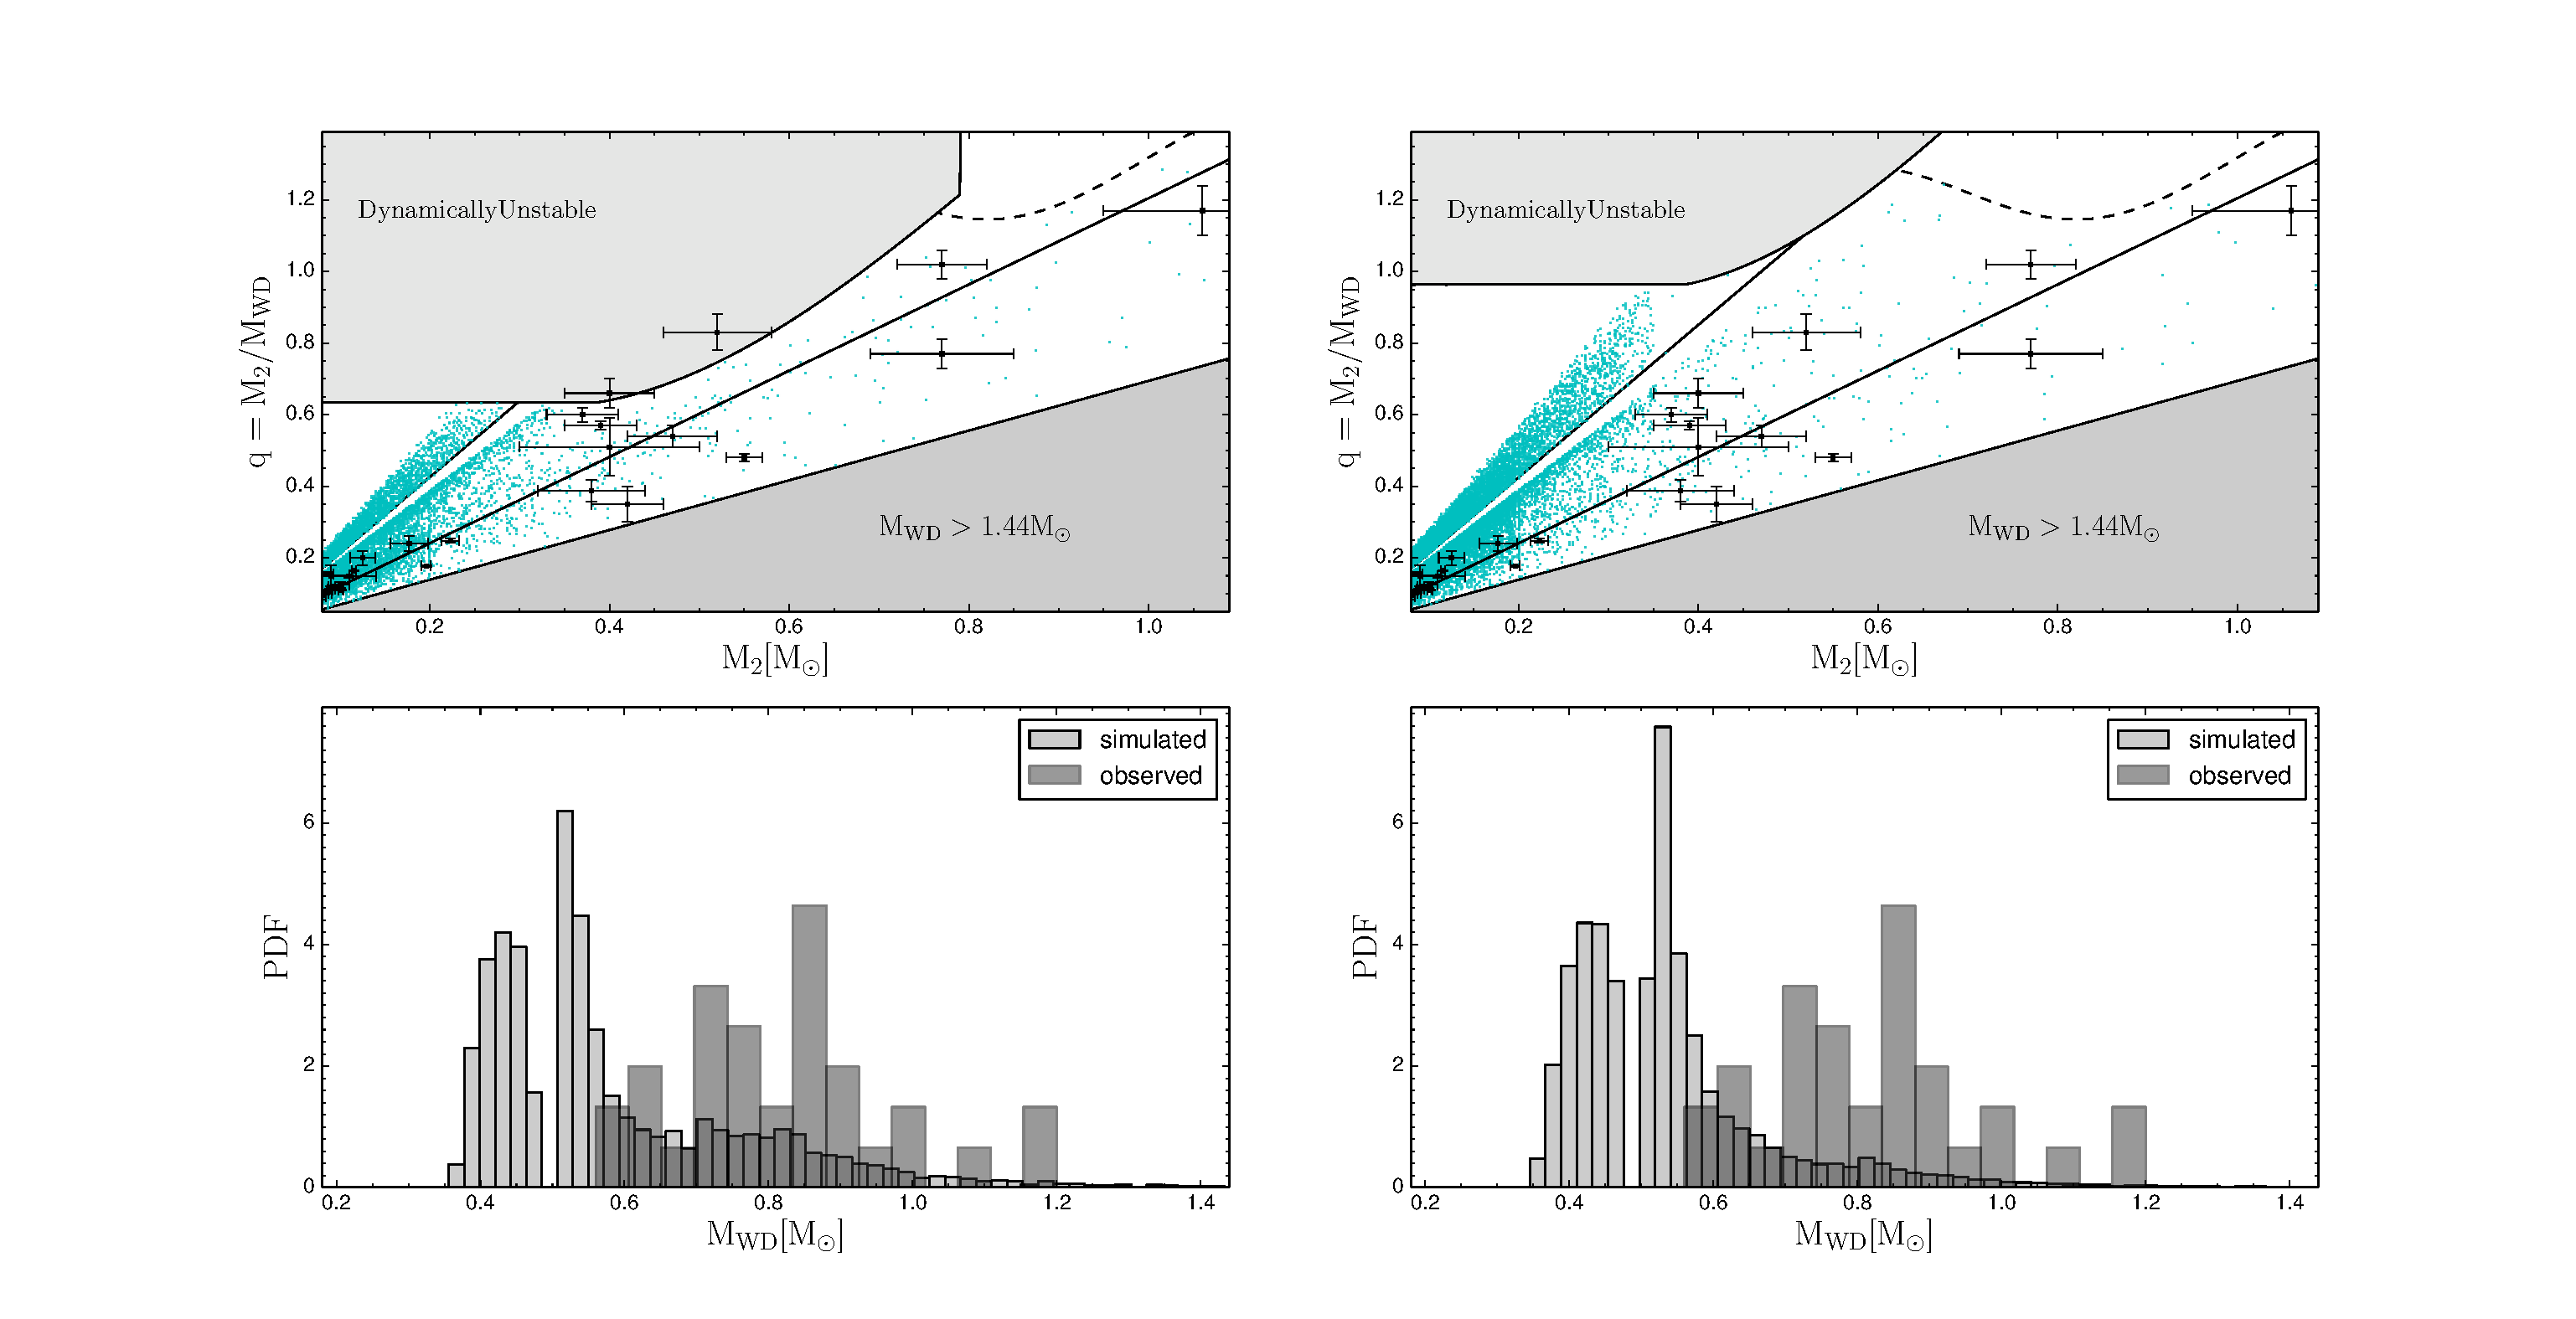
\includegraphics[width=0.8\textwidth,trim={22cm 12cm 0 0},clip]{figures/introduction/Schrieber_figure1.pdf}
    \end{minipage}
    \begin{minipage}[b]{\textwidth}
        \centering
        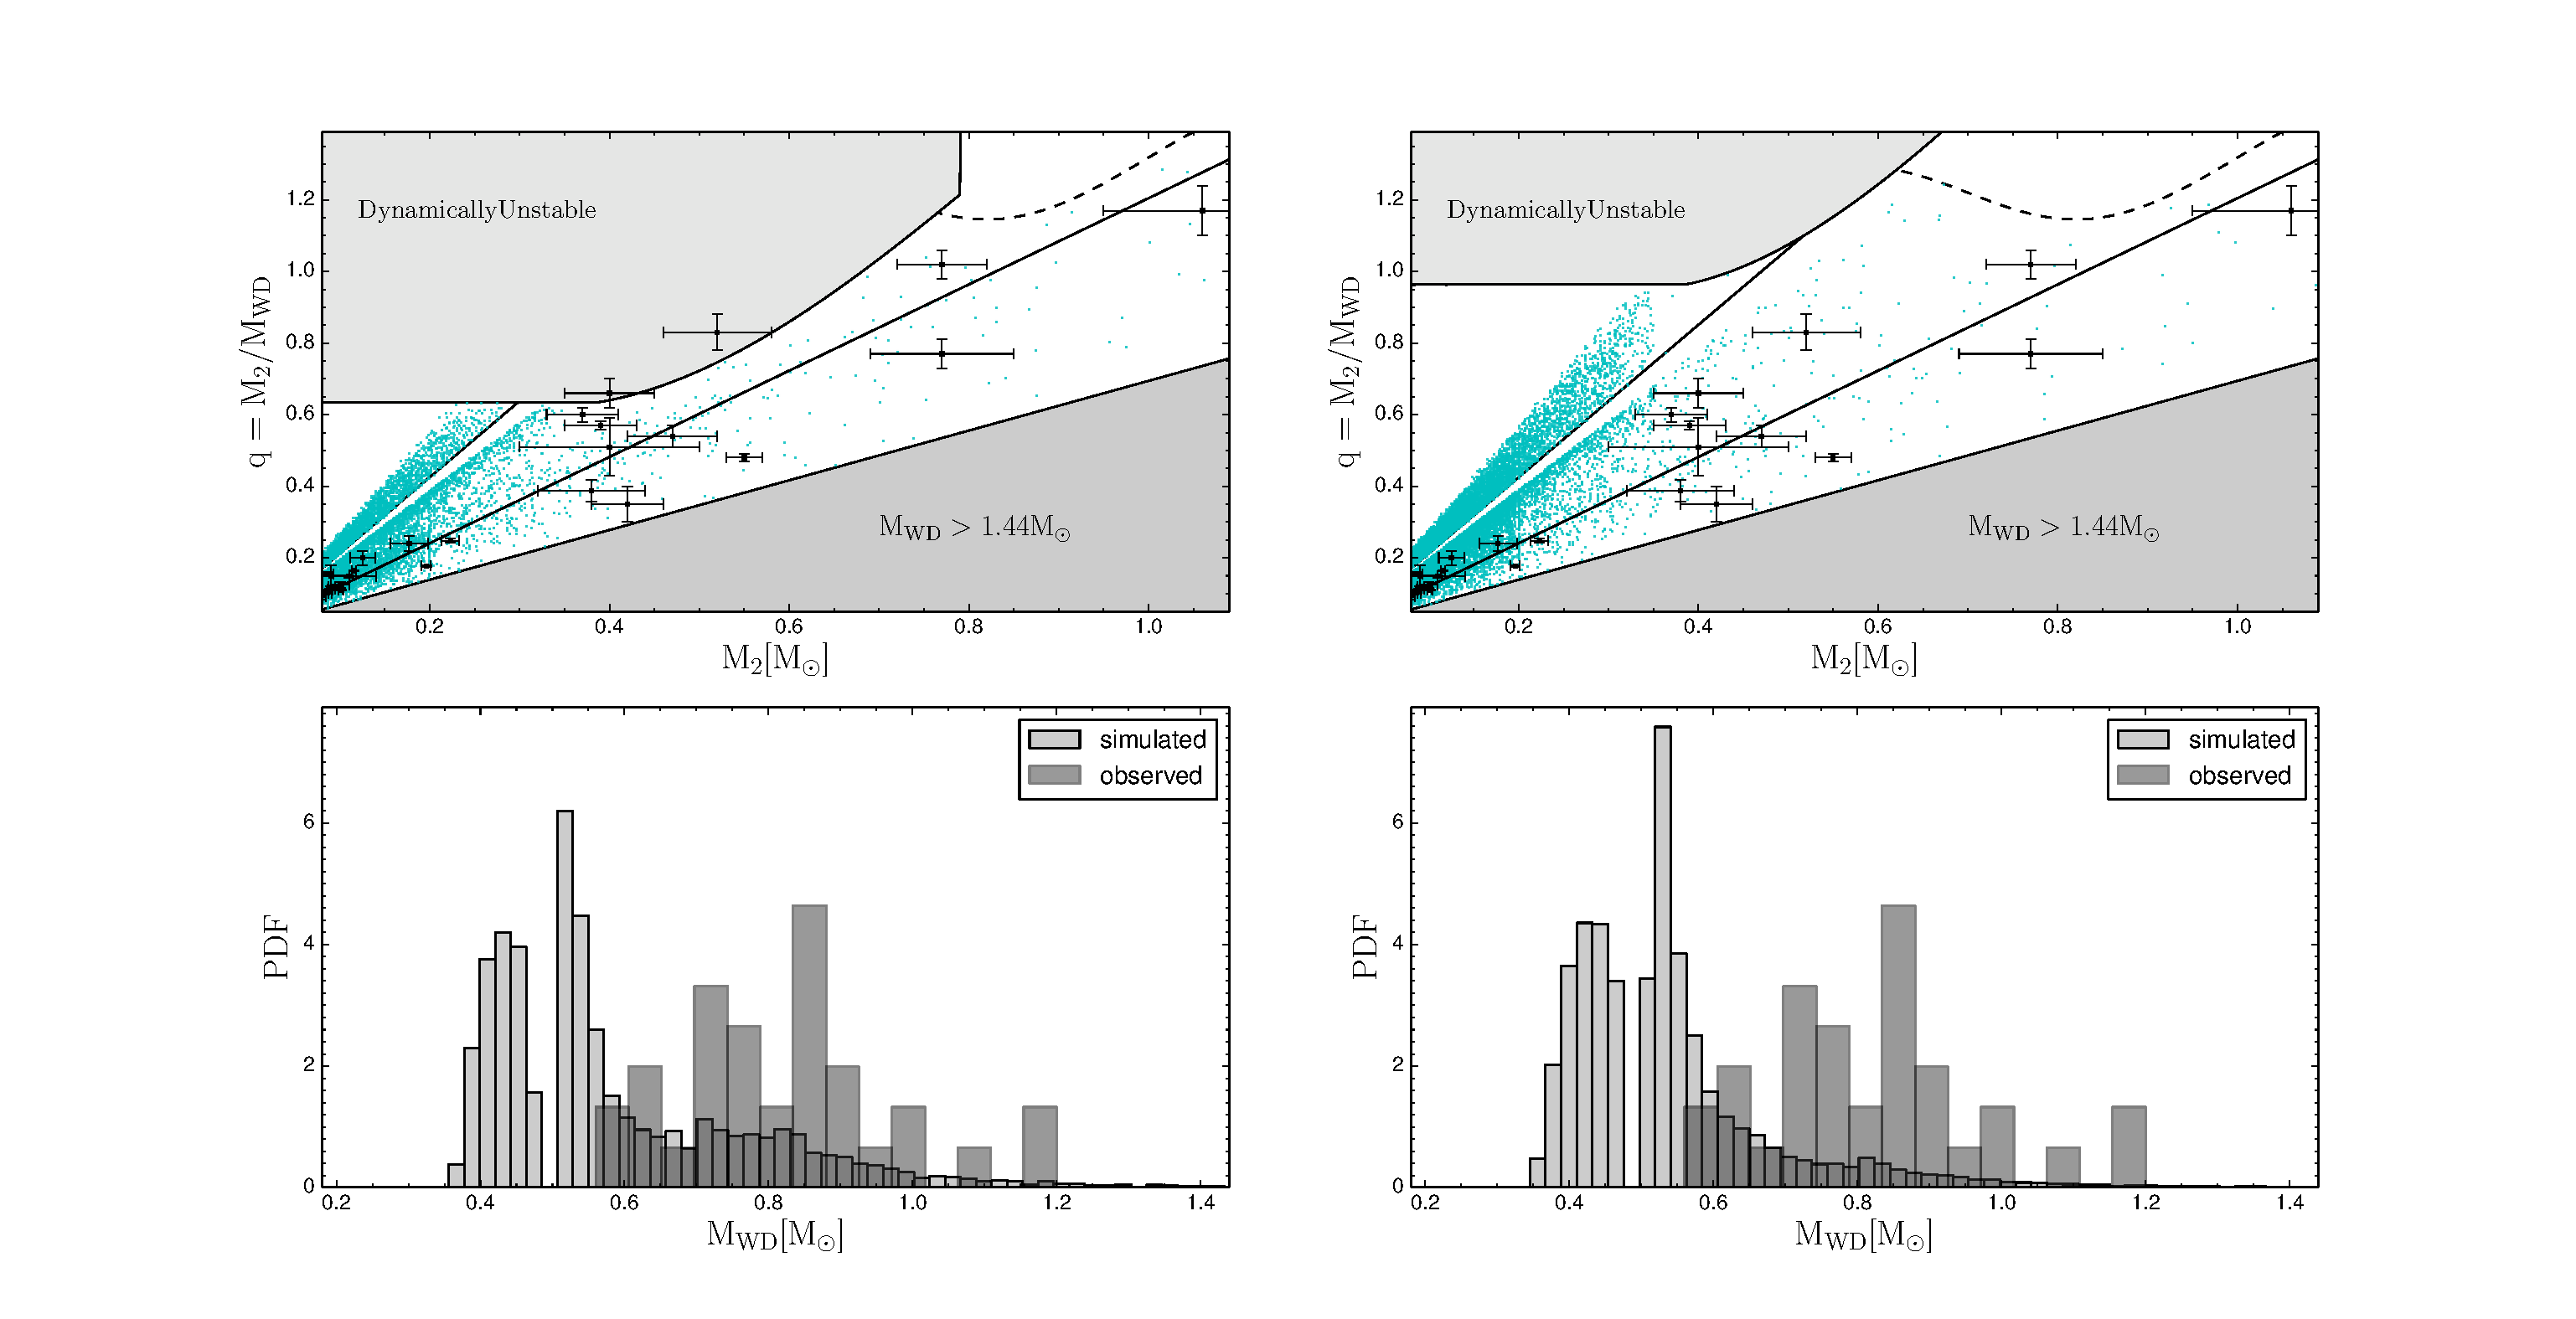
\includegraphics[width=0.8\textwidth,trim={0 12cm 22cm 0},clip]{figures/introduction/Schrieber_figure1.pdf}
    \end{minipage}
    \begin{minipage}[b]{\textwidth}
        \centering
        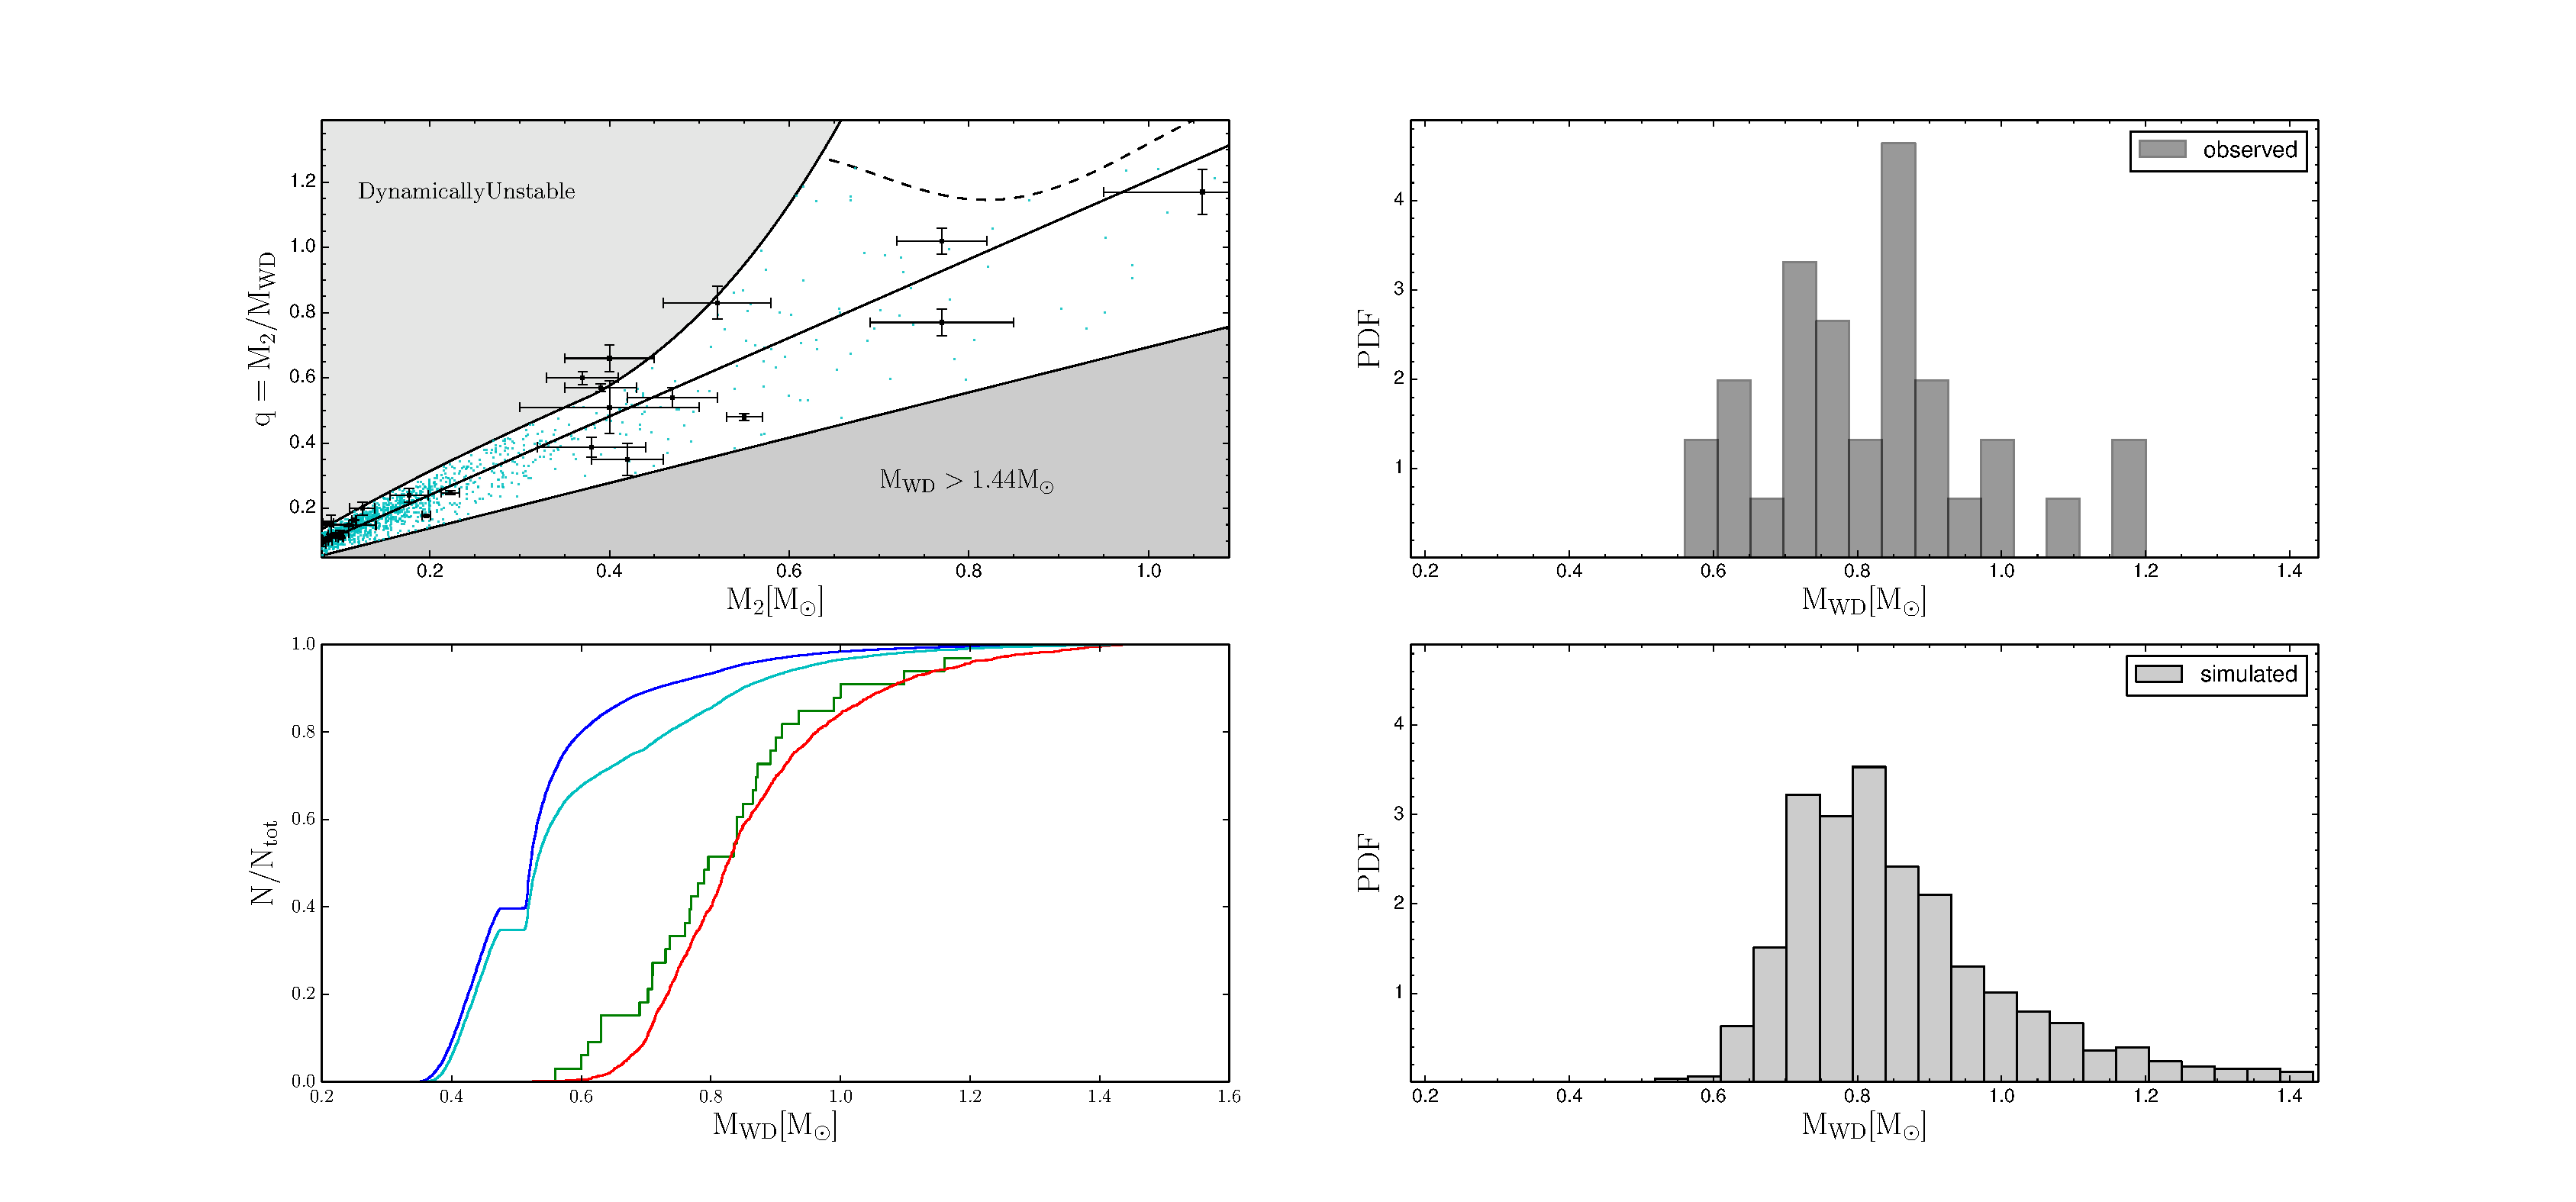
\includegraphics[width=0.8\textwidth,trim={0 11.5cm 24cm 0},clip]{figures/introduction/Schrieber_figure2.pdf}
    \end{minipage}
    \caption{Reproduced from Figure~2 and Figure~3 of \citet{Schreiber2016}. {\bf Black squares} are observed CVs, and {\bf cyan dots} are predicted CV populations. {\it Top} is for a fully conservative CV model, the {\it middle panel} is for the classical non-conservative model, and the {\it bottom panel} is the eCAML results. The $M_{wd} > 1.44 M_\odot$ regions are forbidden, as these white dwarfs exceed the Chandrasekhar limit.}
    \label{fig:introduction:Schreiber 2016 figure 2}
\end{figure}

Some observational evidence for eCAML has recently been uncovered by \citet{Pala2021}, where an inverse correlation between white dwarf mass and mass loss rate was observed. This is in line with Equation~\ref{eqn:introduction:eCAML nu}.
Also, low mass ($<~0.5M_\odot$) helium-core white dwarfs are expected to be formed in binaries, but are frequently observed as singletons. The merger scenario under eCAML provides a neat explanation for this \citep{zorotovic2017}.
In addition, \citet{sparks2021} observed the spectra of CV donors and found significant non-solar abundances,  indicating that after nova outbursts, some of the nova-processed material is retained in the system long enough to be accreted onto the donor, and is supportive both of lower mass white dwarfs having a lower eCAML contribution, and of the donor being immersed in nova material long enough to accrete significant amounts of it.


\subsection{Magnetic Braking}
\label{sect:introduction:magnetic braking}

The M dwarf secondary of a CV will emanate some wind, made up of charged ions, and have some magnetic field which co-rotates with the star.
Consider a blob of charged wind material, moving with some sideways velocity in the plane of the orbit, almost certainly slower than the magnetic field lines.
The blob will interact with the field and be accelerated to co-rotate with them.
This higher velocity causes it to move outwards, to a higher orbit, where the field lines are moving even faster, accelerating the blob more.
As the wind material is accelerated, it exerts a drag force on the magnetic field of the donor and slows its rotation rate.
The close proximity of the binary means that tidal effects are strong, and the donor is spun up again by robbing the orbit of angular momentum, reducing the binary separation and hardening the binary \citep{verbunt1981}.

As an aside, \citet{wickramasinghe1996} presented theoretical motivation that the white dwarfs in CVs can have too strong a magnetic field to allow magnetic braking. Open field lines are necessary for wind to escape the system, so too strong a white dwarf magnetic field can trap the ionised gas in-system, suppressing the wind of the secondary.
Evidence for AML suppression under strong magnetic fields has been found in binary population synthesis models that focus on magnetic CVs \citep{belloni2020}. The models that include magnetic wind suppression under a strong white dwarf magnetic field result in a better fit to key CV observables -- specifically the orbital period distribution, white dwarf temperature distribution, and space density.

When building a magnetic braking model, assumptions must be made about the effects of the magnetic field strength and field geometry, as well as how the wind speed scales with the donor's mass, radius, and rotation rate. The adopted values for these free parameters are tuned to match open cluster data, as open clusters can have their ages determined, and the masses, radii, and rotation rates of the stars contained in them observed (e.g. \citealt{matt2015,garraffo2018a}). The CV community is able to use these findings to inform CV models.
However, the parameter space covered by open cluster data does not cover the parameter space occupied by CVs. Rotation rate is a key variable in magnetic braking prescriptions, but the typical CV rotational period is on the order of a few hours, and singleton M dwarfs are considered extremely fast rotators with periods of a day -- a difference of an order of magnitude. Observations of singletons simply do not reach to the extremely low mass, rapid rotations that are frequently seen in CVs, so we are forced to rely on extrapolation and theory.

This carries with it some major practical issues. One is that whilst the broad effects of magnetic fields is relatively easy to intuit, quantitative physical understanding the mechanics and origins of magnetic fields is difficult, involving fluid dynamics, considering interactions with the accretion disc, and magnetism acting on large systems, which quickly become prohibitive to model and is usually handled with one of a variety of recipes. \citealt{knigge11} contains a detailed compilation of some older approaches, but the decade since has seen a few newer methodologies emerge. Here, two recent magnetic braking prescriptions are described in moderate detail: the \citet{matt2015} prescription, and the \citet{garraffo2018a} prescription. For a more complete, detailed summary of the modern understanding of M dwarf magnetic fields refer to \citet{kochukhov2021}.


\subsubsection{Matt prescription for magnetic torque}
\label{sect:introduction:matt braking}

In \citet{matt2015}, an empirical prescription is derived that relates the torque felt by a low mass main sequence star to that stars' mass, radius, and Rossby number, $Ro$. $Ro$ is a fluid dynamics term for the ratio between the inertial and Coriolis force terms of the Navier-Stokes equations. A small $Ro$ indicates a system dominated by Coriolis effects, and a large $Ro$ indicates that centrifugal and inertial forces dominate. The $Ro$ of a main sequence star can be calculated from its rotation period, $P_{rot}$, and the convective turnover timescale, $\tau_{\rm cz}$.
\begin{equation}
    \label{eqn:introduction:rossby number}
    {Ro} = \frac{P_{rot}}{\tau_{\rm cz}}
\end{equation}
Through $Ro$, the effectiveness of magnetic braking is tied to rotation, which is extremely fast in CVs, and stellar mass and age, which affect $\tau_{\rm cz}$.

\citet{matt2015} make use of observations of stars with masses between $0.15 - 1.3 M_\odot$ and ages of $\sim 10^{6-9}$ yrs, that have had their rotation periods measured. This dataset is used to calibrate a theoretically motivated empirical prescription for magnetic braking. There is some evidence for a saturation of magnetic activity below a critical Rossby value (a.k.a. above a critical rotational period) \citep{reiners2009}, where magnetic activity seems to no longer respond to changes in rotation. \citet{matt2015} therefore adopt two relationships for torque, $T$, modulated by an empirical value, $p$,
\begin{equation}
    T = -T_0 \bigg( \frac{\tau_{\rm cz}}{\tau_{cz,\odot}} \bigg)^p \bigg( \frac{\Omega_{*}}{\Omega_{\odot}} \bigg)^{p+1}
\end{equation}
for the unsaturated regime, and
\begin{equation}
    T = -T_0 \chi^p \bigg( \frac{\Omega_*}{\Omega_\odot} \bigg)
\end{equation}
in the saturated regime. In both cases, $p$ is assigned as $p = 2$ in order to agree with the most common literature spin-scaling prescription, $T \propto \Omega_*^3$.
$\chi$ is the inverse critical $Ro$ for saturation, for which \citet{matt2015} adopt a value of $10$.
The rotation rates of the donor and the sun are $\Omega_{*,\odot}$ respectively, and $T_0$ is given by a function of mass and radius,
\begin{equation}
    T_0 = 9.5 \times 10^{30} {\rm erg} \bigg(\frac{R_*}{R_\odot} \bigg) \bigg(\frac{M_*}{M_\odot} \bigg)
\end{equation}

The authors take observations of two clusters, the $\sim 5$ Myr old ONC cluster and the $\sim 580$ Myr old Praesepe cluster, and use the first as initial conditions and the second as target distribution to reproduce. Figure~\ref{fig:introduction:Matt 2015 figure 2} is taken from \citet{matt2015}, and compares the initial and final conditions of their synthetic cluster model compared to these two boundary conditions. During the first few tens of Myrs of this model, the stars in the synthetic cluster are spun up as they contract, lowering their periods by factors of $\sim 5-10$. After this initial phase, which is much shorter than the spin down timescales, the more long-term spin evolution begins.
\begin{figure}
    \centering
    \begin{minipage}[b]{\textwidth}
        \centering
        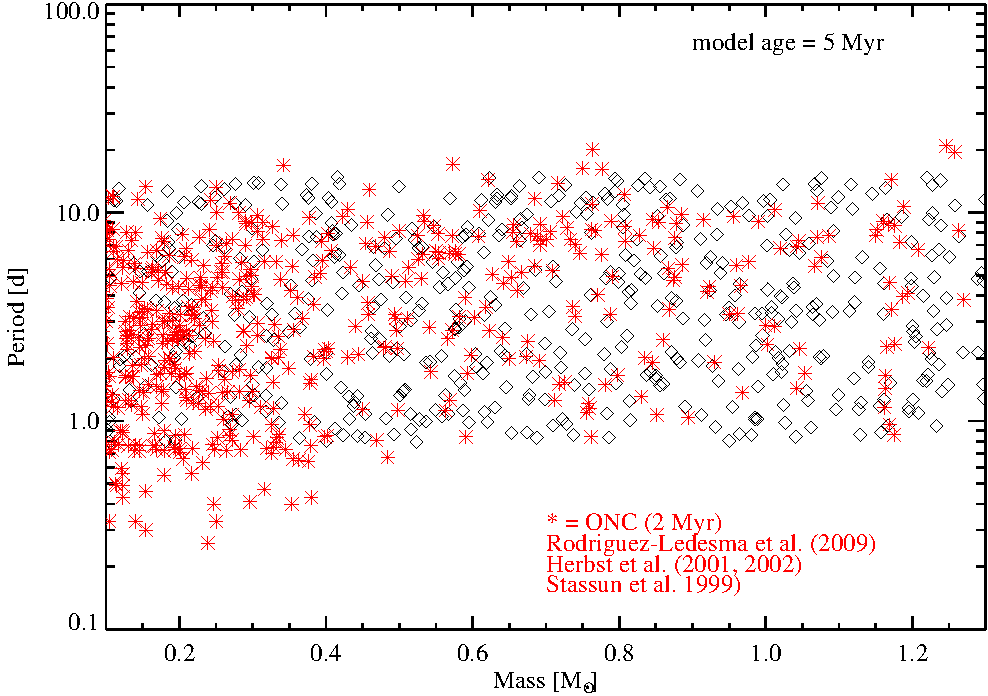
\includegraphics[width=0.8\textwidth]{figures/introduction/matt_2015_fig2a.pdf}
    \end{minipage}
    \begin{minipage}[b]{\textwidth}
        \centering
        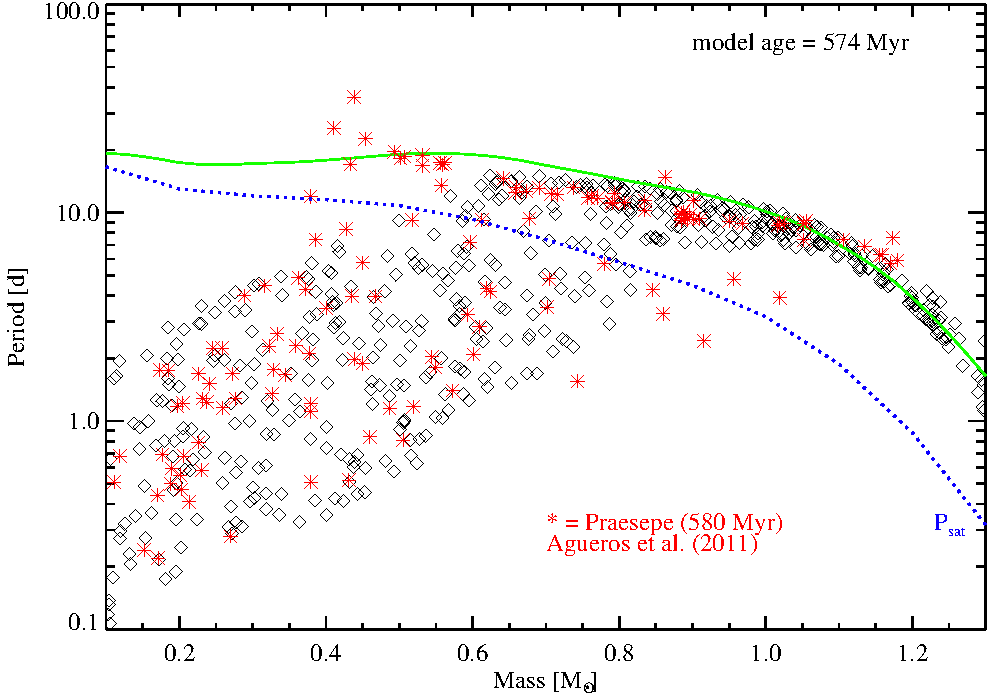
\includegraphics[width=0.8\textwidth]{figures/introduction/matt_2015_fig2b.pdf}
    \end{minipage}
    \caption{Figure taken from \citet{matt2015}. {\bf Red crosses} are observations of the ONC ({\it top}) and Praesepe ({\it bottom}) cluster stars. {\bf Black diamonds} are synthetic cluster stars. In the bottom panel, the {\bf solid green line} is the theoretical asymptotic spin rate of unsaturated stars and the {\bf dotted blue line} delimits magnetically saturated and unsaturated stars.}
    \label{fig:introduction:Matt 2015 figure 2}
\end{figure}

The agreement between the synthetic cluster and the Praesepe cluster at 574 Myrs is impressive. Above $\sim 0.8 M_\odot$, stars converge on a single narrow mass - period track just as is seen in the observations, and the large scatter below $\sim 0.8 M_\odot$ is also reproduced. Also, just as is seen in the cluster observations of Praesepe, the fastest rotators are those with the lowest masses. Both of these features arise from the transition from saturated braking, to unsaturated braking \citep{matt2015}.

At formation, almost all stars are experiencing saturated magnetic braking. The single narrow track arises from higher mass stars spinning down faster than lower mass stars, moving them off the much less efficient saturated braking regime sooner. The pile-up of systems then produces the narrow track. The mass dependancy of this track comes from the fact that spin-down timescale in the saturated regime is shorter for higher mass stars.
The broad population of low mass rapid rotators is a direct result of the broad initial conditions, which span an order of magnitude themselves, and the longer spin-down time of lower mass stars in the saturated regime allowing them to remain at high rotation rates for longer.

However, this model does fail in a few key respects. In the bottom panel of Figure~\ref{fig:introduction:Matt 2015 figure 2}, a small population of very slow rotators can be seen at $\sim 0.4 M_\odot$. The slower rotation rates of these stars suggests an alternative spin-down mechanism. The inverse problem is seen at $\sim 0.7 M_\odot$, where a handful of stars are seen rotating {\it faster} than predicted by any of the synthetic cluster stars, suggesting that magnetic braking is not as effective in their case.
More importantly for the CV field, the parameter space of CVs is completely uncovered, as CVs have rotation periods of $< 0.2$ days, and the systems that this work concerns have periods of $\lesssim 0.07$ days. Whilst this would firmly place CVs in the saturated regime, there is evidence of a `supersaturated' regime at extreme rotation periods that may be relevant to CV donors \citep{James2000, Wright2011, Argiroffi2016}. This possibility is also noted by \citet{Gossage2021} when outlining best practice use of this prescription in the stellar evolution code MESA, though the subject is not a settled matter and competing evidence for the {\it lack} of supersaturation has been reported by \citet{jeffries2011}.


\subsubsection{Garraffo prescription for magnetic torque}
\label{sect:introduction:Garraffo magnetic braking prescription}

The \citet{garraffo2018a} model considers the morphology of the magnetic field to also be important to the strength of magnetic braking, based on the work by \citet{garraffo2015}. The primary justification for this inclusion is observations of open clusters of a known age, where a bimodality is seen in the rotation rates of stars of similar masses. Some stars appear to be fast rotators, and some are slow rotators, and there is a dearth of systems between the two.
Previous attempts to model this bimodality have relied on an unexplained transition between an efficient braking state, and an inefficient braking state \citep{spada2011,reiners2012, gallet2013}, and \citet{garraffo2018a} expand on this by offering a shift in magnetic field morphology as the underlying trigger.

Their formalisation of this is based on two assumptions. They assume that stars with a dipolar magnetic field follow a known spin-down law, with a mass dependence reflecting $\tau_{\rm cz}$ \citep{skumanich1972}. Second, they assume that there is some relationship between field morphology and stellar spin rate. Specifically, that stars rotating more rapidly have more complex magnetic fields. This is formalised via an AML rate, $\dot J$,
\begin{equation}
    \dot J = \dot J_{\rm dipole}Q_J(n)
\end{equation}
where $\dot J_{\rm dipole}$ is the dipole loss under the Skumanich law, $\dot J_{\rm dipole} \propto \Omega^3 \tau_{\rm cz}$. $Q_J$ is a modulating factor that encapsulates the field complexity at the stellar surface, and is controlled by the complexity factor, $n$, which is a function of $Ro$. \citet{garraffo2016} derive an equation for $Q_J$, based on fitting the results of magneto-hydrodynamic simulations with varying field complexities.
\begin{equation}
    \label{eqn:introduction:garraffo complexity modulation}
    Q_J(n) = 4.05 e^{-1.4n} + \frac{n-1}{60Bn}
\end{equation}
Where $B$ is the magnetic field strength at the stellar surface. As the second term is only significant for $n > 7$, \citet{garraffo2018a} consider $n = 7$ as the maximum complexity, and consider only the first term of this relation. This is the equivalent of the saturation of magnetic braking, but here is contingent on field complexity rather than $Ro$.

\citet{garraffo2018a} suggest the following relation between $Ro$ and $n$,
\begin{equation}
    \label{eqn:introduction:garraffo field complexity}
    n = 1 + \frac{x}{Ro} + (y \cdot Ro)
\end{equation}
where $x$ and $y$ are free parameters, chosen to fit observations of open clusters. The three terms reflect three aspects of the magnetic braking model - the minimum complexity is defined as $n \equiv 1$, the first factor encodes stars with small $Ro$ having large $n$ (e.g. young, fast rotators), and the third term gives stars with large $Ro$ similarly large $n$ to explain the observed population of old rapid rotators that appear to have experienced minimal spin-down \citep{vanSaders2016}.
This prescription explains the AML of a star as purely a function of $Ro$.

Similarly to \citet{matt2015}, \citet{garraffo2018a} run a population synthesis model to compare to observations using initial conditions taken from the 13 Myr old h Persei cluster \citep{moraux2013}, but the authors show that differences between alternative initial conditions do not survive longer than 200 Myrs. Observations of stellar rotation periods and colour from several clusters with known ages are then compared to the synthetic population.

The resulting distribution does recover the Skumanich bifurcation observed in open clusters, reproducing the fast and slow rotating populations and the gap between them, though the large uncertainty in the age of the cluster does introduce some discrepancy.
In addition, the synthetic cluster does not consider the effects of close binary stars, which will affect the spin-down rate through tidal effects. However, this effect is ignored by the author, as there is evidence that the binary fraction in open clusters is low \citep{meibom2007}.
The mass dependency of this track is also reproduced by the model, and Figure~\ref{fig:introduction:garraffo 2018a fig 4}.
\begin{figure}
    \centering
    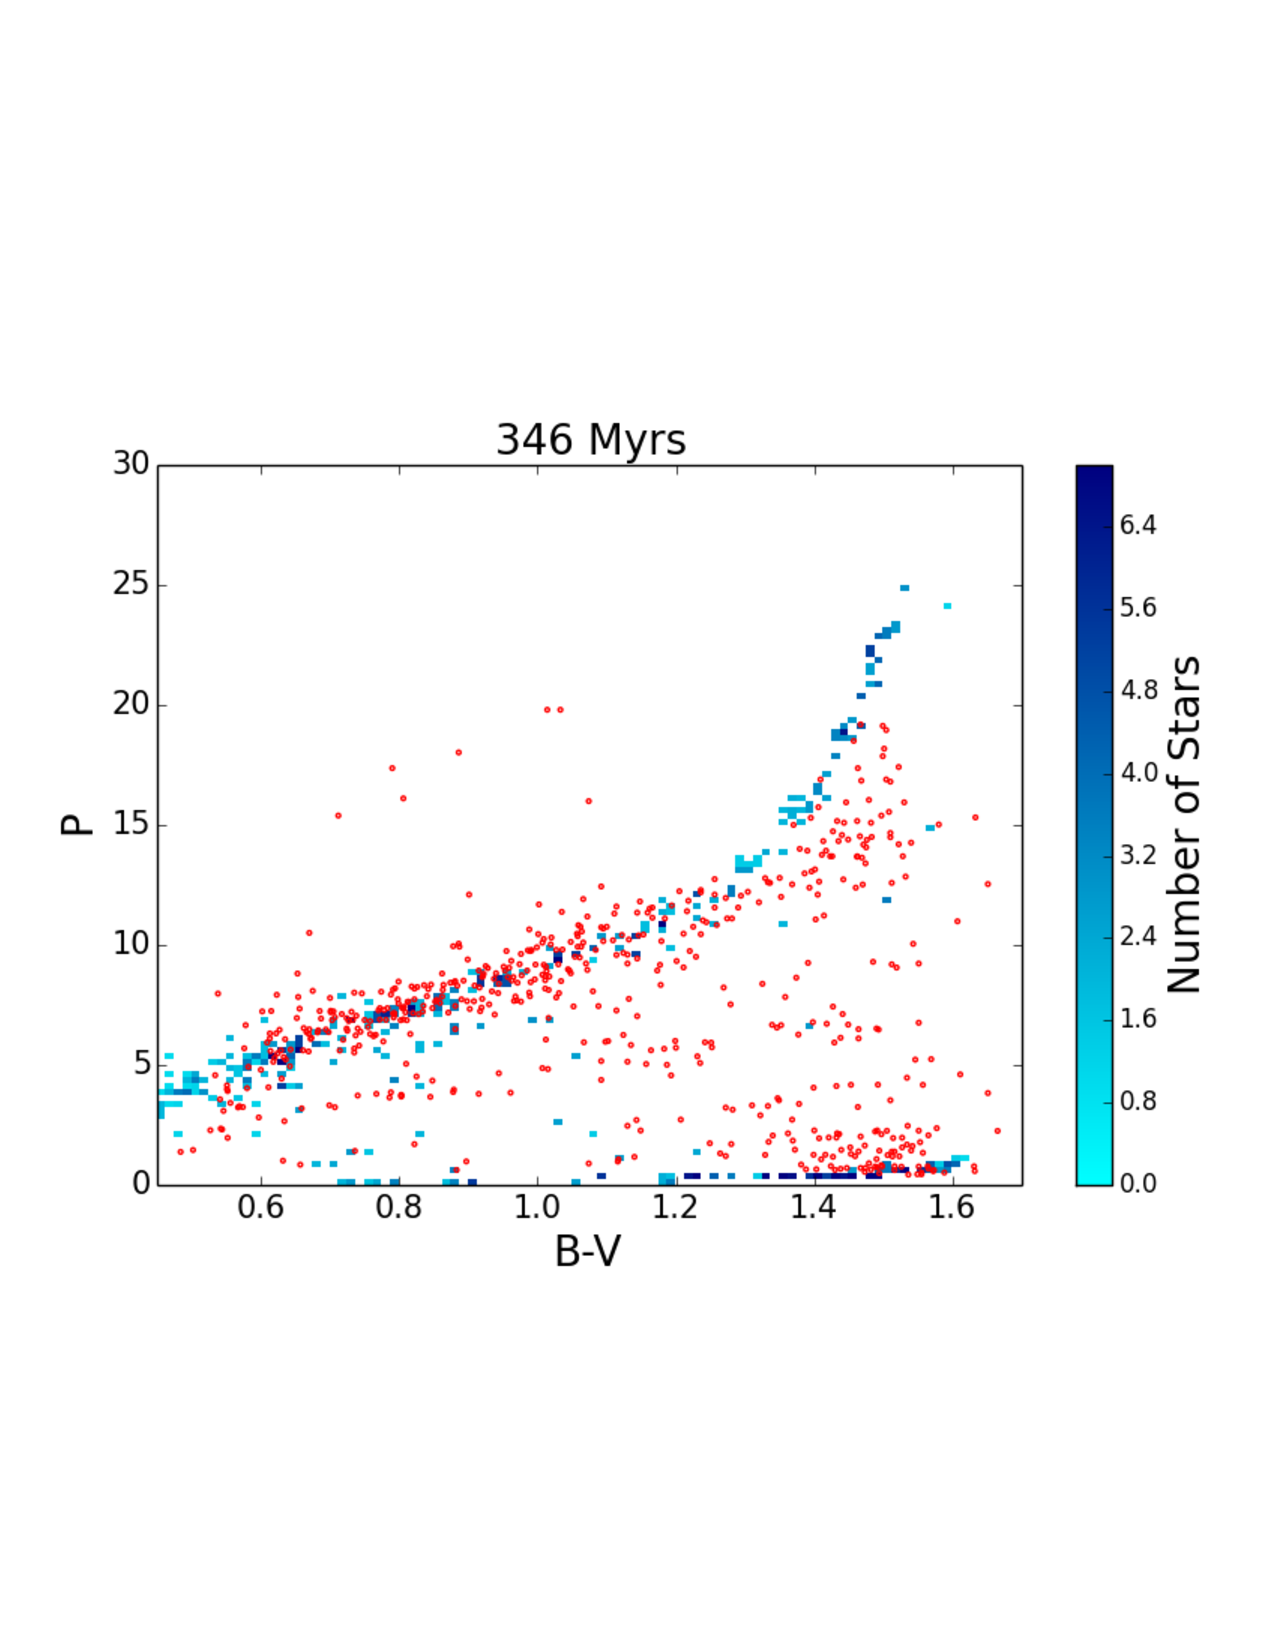
\includegraphics[width=0.7\textwidth, trim={0 5cm 0 5cm}]{figures/introduction/garraffo2018_M37_346_hPer.pdf}
    \caption{Example comparison between synthetic and observed cluster populations taken from \citet{garraffo2018a}. {\bf Red points} are observations of M37, which has its age measured at $\sim 346 - 550$ Myrs. {\bf Blue points} are the probability distribution of the synthetic cluster population from \citet{garraffo2018a}.}
    \label{fig:introduction:garraffo 2018a fig 4}
\end{figure}

The \citet{garraffo2018a} prescription is simpler in concept than the \citet{matt2015} prescription, and both prescriptions perform well. However, neither formulation covers the parameter space of CV donors, and both are semi-empirical with some arbitrary decisions made in order to fit open cluster data. This makes both approaches highly vulnerable to extrapolation errors and difficult to trust in the context of CV evolution, especially in the short period regime.


\subsubsection{Comparisons to the Rappaport, Verbundt and Joss model}

We can examine the differences between these prescriptions in the case of CV evolution by applying them to a donor evolutionary track, and \citet{knigge11} has constructed a donor sequence using their own models that reasonably accurately reproduces observations. The masses, radii, and periods along the sequence are given, so the would-be effects of the magnetic braking prescriptions described above can be calculated. In addition to the two previously discussed prescriptions, the default MESA \citep{Paxton_2015} magnetic braking prescription \citep{rappaport1983} is included. This prescription includes a magnetic braking index, $\gamma$,
\begin{equation}
    \dot J = -3.8\times10^{-30} M R_\odot^4 \bigg( \frac{R}{R_\odot} \bigg)^\gamma \omega^3\  {\rm dyn\ cm}
\end{equation}

Note that in the specific case of CVs, period and radius are synonymous with one another due to the requirement that the donor is in contact with the Roche lobe, and is tidally locked.

\begin{figure}
    \centering
    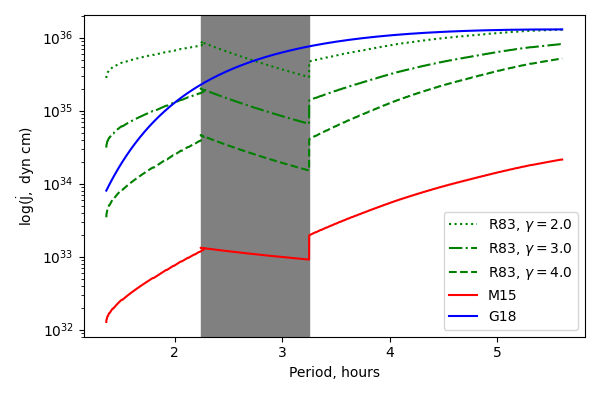
\includegraphics[width=\textwidth, trim={1cm 0 0 0}]{figures/introduction/rappaport_garraffo_matt_magbraking_period.png}
    \caption{Showing the AML rates, $\dot J$, of three magnetic braking prescriptions, applied to the masses, radii, and spin periods of the `standard' CV donor track of \citet{knigge11}. The {\bf vertical shaded region} shows the period gap, corresponding to the mass at which \citet{knigge11} enforces the period gap to occur. {\bf Green lines} show the \citet{rappaport1983} magnetic braking prescription, which is the default used in MESA \citep{Paxton_2015}. The {\bf red line} shows the \citet{matt2015} prescription, and the {\bf blue line} shows the \citet{garraffo2018a} prescription.}
    \label{fig:introduction:rappaport garraffo matt magnetic braking}
\end{figure}

Figure~\ref{fig:introduction:rappaport garraffo matt magnetic braking} shows how the \citet{matt2015} magnetic braking prescription compares to the default MESA magnetic braking prescription, from \citet{rappaport1983}. All prescriptions see a discontinuity at $0.2M_\odot$, where \citet{knigge11} imposes the magnetic braking cutoff and the donor contracts to its equilibrium radius.

The differences between the three prescriptions is clear in both the overall strength of the prescriptions, but also in how they evolve with mass. All the prescriptions shown decrease at lower masses, but at different rates. In the context of CV evolution, a different dropoff rates of magnetic braking would alter the shape of the donor mass-radius sequence, so observations of CV donors should be able to allow us to evaluate the effectiveness of different braking prescriptions.

Note that the AML from magnetic braking predicted by \citet{matt2015} is $\sim 2$ orders of magnitude lower than the braking commonly required to calculate CV evolution. This is a consequence of tuning their braking model's free parameters to open cluster rotation rates, and the effects of this under-estimation is explored by \citet{andronov2003}. This problem is avoided in the case of \citet{garraffo2018a,garraffo2018b}, by using different values of their free parameters for open cluster stars and CVs.


\section{This work}
\label{sect:introduction:this work}

The primary focus of this work is in expanding the sample of well-characterised CV donors, which remains small (less than 40 systems in total). Whilst this sample is augmented by the large number of donors characterised using the superhump excess technique (\S\ref{sect:introduction:SU UMa}), eclipse modelled systems are preferable due to the small number of robust assumptions that need to be made. The specific focus is on characterising systems with short periods, and therefore low mass donors, in an attempt to increase the number of well-characterised period bouncing systems. I characterise an additional 15 CV systems below periods of $\lesssim 2.5$ hours.

The secondary goal is then to take this larger sample, and make comparisons to CV evolutionary models below the period gap. By comparing observed data with the predicted donor masses and radii across the range of periods, the long-term baseline AML rate can be inferred for a given system. As these short-period systems are expected to only evolve under gravitational braking, but are known to experience some excess AML above this, various empirical prescriptions for excess AML as functions of the CV system parameters can be built and serve as a diagnostic for the physical motivation of the excess AML.

\todo{When the rest of the thesis is written, outline the structure of the document as a whole. i.e. in section XX I will YY, in section ZZ I will...}


\chapter{Observations and observational techniques}
% Chapter Template

\label{chpt:observations and observational techniques} % for referencing this chapter elsewhere, use \ref{chpt:label}
\lhead{\emph{Observations, and observational techniques}} % This is for the header on each page - perhaps a shortened title

For CVs with a sufficiently high inclination ($\gtrsim 80 \deg$, depending on mass ratio) the donor will eclipse all other components of the system in quick succession, once per orbit. Observing and modelling these eclipses, with knowledge of the orbital period and the temperature of the white dwarf, can yield a thorough characterisation of the CV. The methodology for this characterisation is described in detail in \S\ref{chpt:modelling and techniques}, but essentially relies on extracting the white dwarf temperature and radius from the white dwarf colours and system parallax, and combining the white dwarf radius with the timing of eclipse features to find the component masses, donor radius, and orbital separation. Hence, to properly characterise a CV, we need flux-calibrated, high time resolution, multi-colour photometery of the target. 

The work of this thesis has made extensive use of three instruments: ULTRASPEC, ULTRACAM, and HiPERCAM.
These are time-series photometric imaging cameras, capable of taking high-cadence images of the night sky in one, three, or five colours, respectively. Crucially, HiPERCAM and ULTRACAM make their multi-colour images simultaneously, which removes the possibility of changes in brightness in the disc or bright spot polluting the white dwarf colour measurement. The eclipses we observe typically span around 30 minutes and need to measure flux changes on timescales of a few seconds to be useful for analysis, and these three cameras are ideal for this task.


\section{Instruments}

The cameras used were mounted on several telescopes across the decade of our observations. These were the Gran Telescopio de Canarias (GTC) on La Palma (with HiPERCAM), the Thai National Telescope (TNT) with ULTRASPEC, the New Technology Telescope (NTT) in Chil\'e (with ULTRACAM). Prior to [YEAR]\todo{When was ULTRACAM taken off the WHT? 2014, I think?}, ULTRACAM was hosted on the William Herschel Telescope (WHT), also on La Palma. 


\subsection{HiPERCAM}

HiPERCAM is an impressive quintuple-beam optical imaging camera that saw first light on the GTC in 2018, and is sensitive to wavelengths between $320 - 1060 \rm nm$ \citep{dhillon2021}. 
This camera has a series of dichroic beamsplitters, that sequentially pick off the $u_{\rm sup}, g_{\rm sup}, r_{\rm sup}, i_{\rm sup}, z_{\rm sup}$ bands and funnel each into dedicated cameras that use highly sensitive, low readout noise electron-multiplying CCDs. 
These Super SDSS filters are specifically designed for HiPERCAM to match the classic SDSS band cutoff wavelengths \citep{fukugita1996}, but allow a higher throughput and so give a more sensitive instrument. 
However, this improvement is not constant across the bands, shown in Figure~\ref{fig:observations:superSDSS throughput comparison}, resulting in a small difference between colours observed with HiPERCAM and SDSS. 
Unfortunately, as our calibrating standard stars are reported in the classic SDSS photometric system, some work was necessary to color-correct the HiPERCAM observations, which is described in detail in \S\ref{sect:observations:colour correction method}.
\begin{figure}
    \centering
    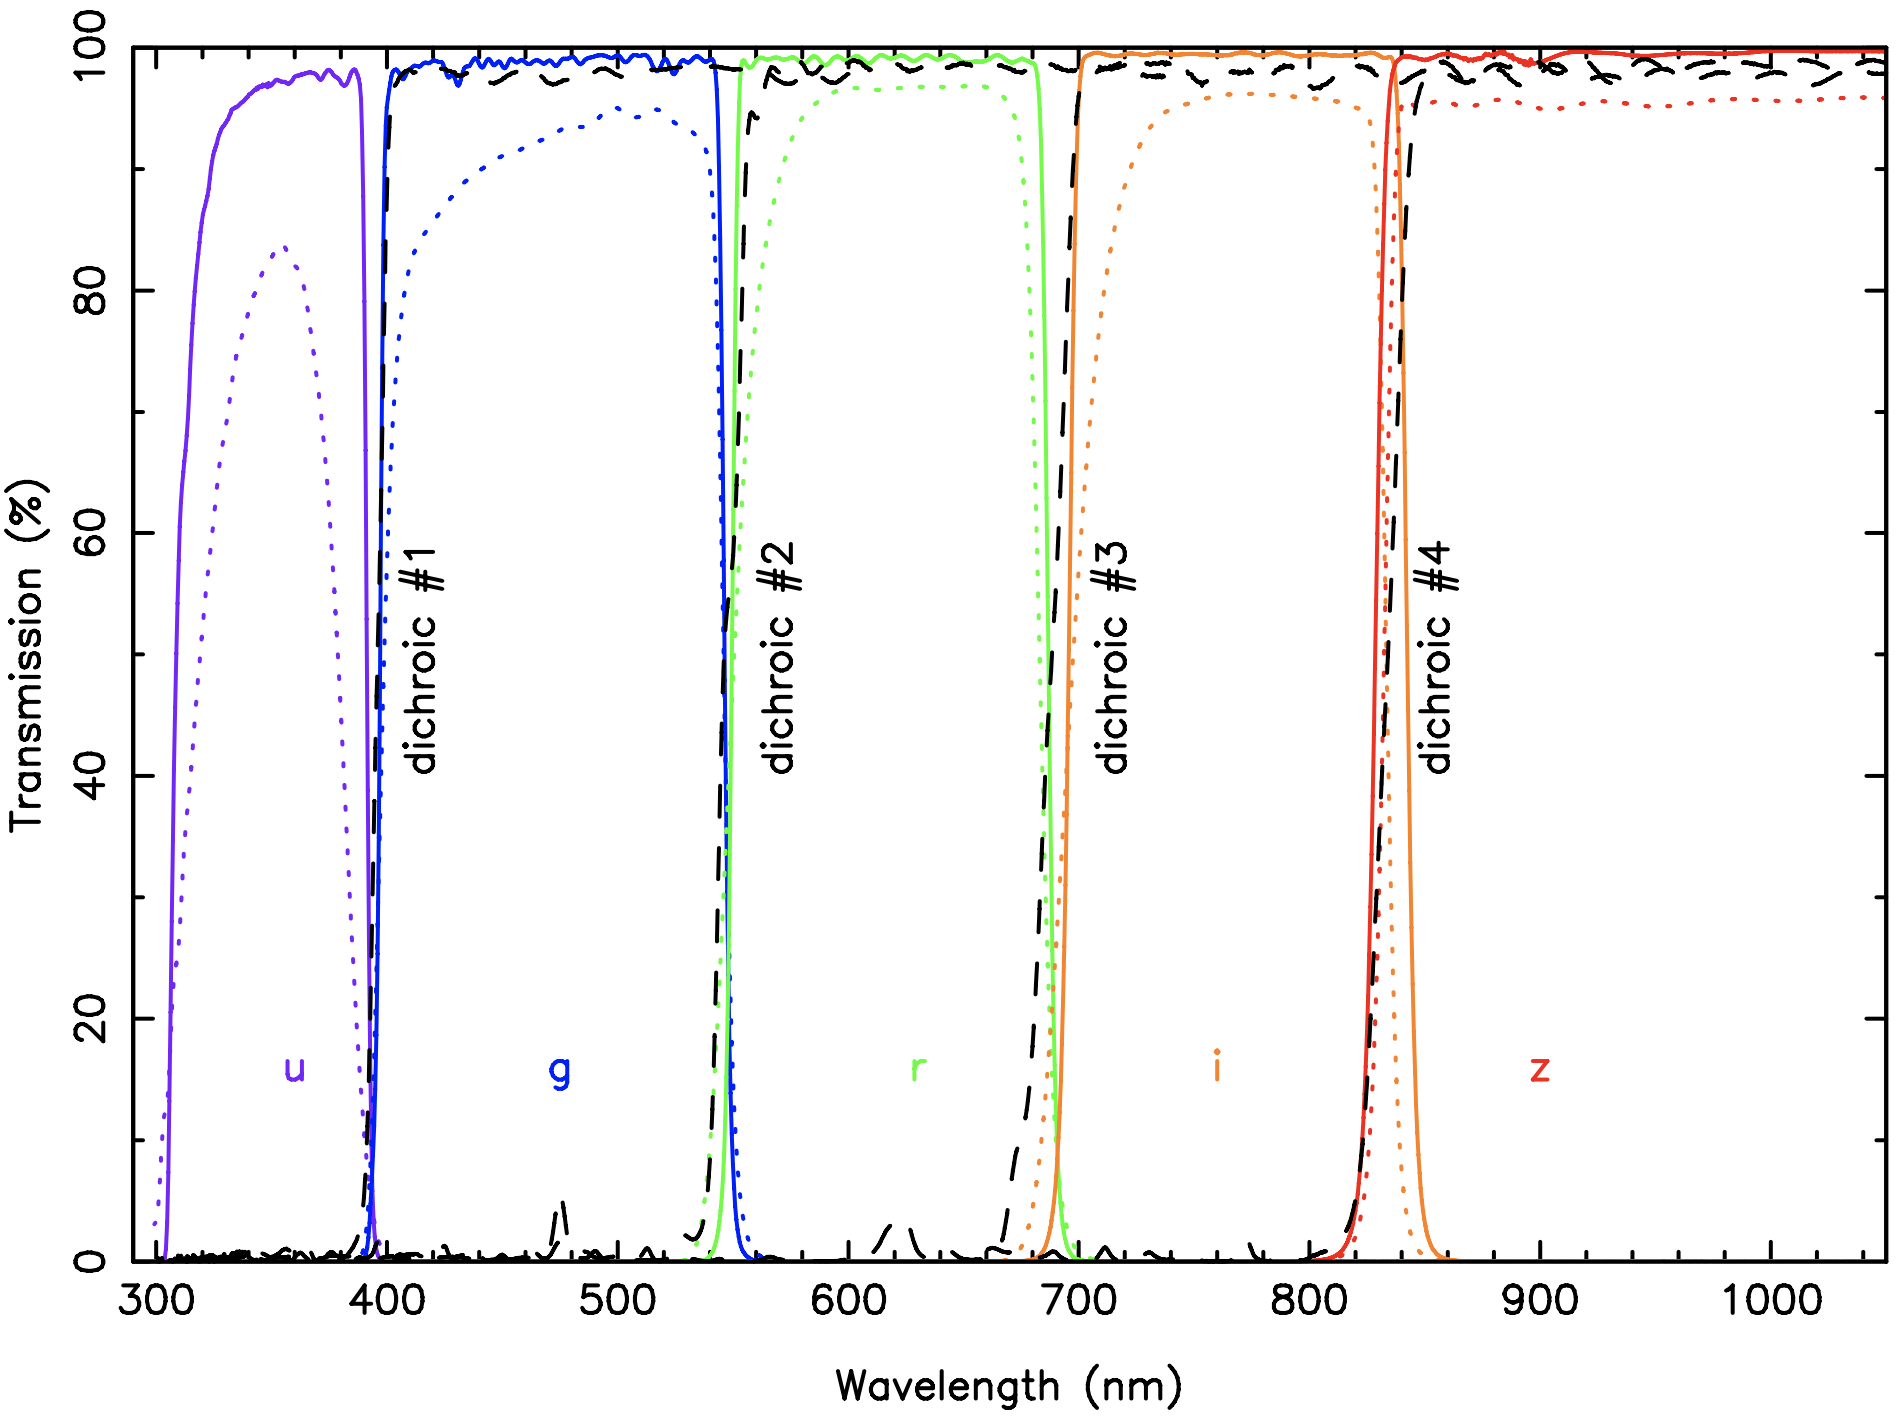
\includegraphics[width=0.7\textwidth]{figures/observations/plot_dichs_supersdss_asbuilt_v3.png}
    \caption{Taken from \citet{dhillon2021}. Transmission profiles of the as-built HiPERCAM dichroic beamsplitters (dashed lines), the HiPERCAM standard SDSS filters (dotted lines), and the HiPERCAM Super SDSS filters (solid
    lines).}
    \label{fig:observations:superSDSS throughput comparison}
\end{figure}

On the GTC, HiPERCAM is capable of detecting sources down to $g_{\rm sup} \sim 23$ in exposures of only a second, and can achieve $g_{\rm sup} \sim 28$ with an hour of exposure. This has allowed us to make excellent observations of fainter CVs than previous studies \citep{McallisterThesis}, with low mass donors and short periods. In addition, HiPERCAM is capable of incredibly fast framerates of up to $\sim 1000 \rm Hz$, though this capability was not used for this work. 
However, as part of the effort to achieve this framerate by reducing dead-time between frames HiPERCAM is capable of exposing a frame and {\it simultaneously} reading out the previous image. 
This is achieved by splitting the photodetector in half, and masking one side. When a frame is finished exposing, it is shuttled across to the masked side (a rapid process, $6.8 - 7.8$ms) and can be read out during the next exposure time. This is a significant benefit when resolving the large, rapid changes in flux during the ingresses and egresses of CV eclipses.


\subsection{ULTRACAM}

ULTRACAM is a three-beam optical imager sensitive to wavelengths between $\sim 300 - 1100 \rm nm$, and is the direct predecessor to HiPERCAM \citep{dhillon2007}. 
It is similarly built for high-speed photometric studies, but is `only' capable of framerates of $\sim 500 \rm Hz$ in three of its five bands. 
It uses the same split-frame readout technique to HiPERCAM, though uses more typical CCDs rather than HiPERCAM's electron-multiplying CCDs. Observing an object in more than three bands requires multiple observing runs, and manually swapping the filters.

ULTRACAM was originally commissioned with SDSS-like $u',g',r',i',z'$ filters, that match the SDSS closely and did not necessitate colour-term corrections. However, in [YEAR] \todo{When did we move to super SDSS on ultracam? 2018?} ULTRACAM was upgraded to use the same Super SDSS photometric system used by HiPERCAM. When necessary, observations were translated to the classic SDSS system as described in \S\ref{sect:observations:colour correction method}. 


\subsection{ULTRASPEC}

Finally, the ULTRASPEC instrument was occasionally used to supplement ULTRACAM and HiPERCAM observations. ULTRASPEC was originally commissioned as a spectrographic cousin of ULTRACAM, using again a split-frame design, with electron-multiplying CCDs \citep{dhillon2014}. 
After a brief proof-of-concept trial as a photometric imager in June 2009, ULTRASPEC was modified to a full-time imaging instrument and mounted on the 2.4m TNT in November 2013, and is now operated by the National Astronomical Research Institute of Thailand (NARIT).

This is a single-colour instrument that uses the $u',g',r',i',z'$ filters, in addition to a wide-band KG5 filter that is approximately equivalent to $u' + g' + r'$. It is also the slowest of the three cameras, but is still capable of high framerates up to $\sim 200 \rm Hz$. However, as ULTRASPEC is a somewhat less powerful instrument, it proved useful in two significant respects - to gauge the viability of CV systems before dedicating more valuable HiPERCAM and ULTRACAM observing time (e.g. testing the visibility of eclipse features, checking if a CV is undergoing an outburst), and in acquiring or refining measurements of orbital period.


\section{Data reduction}
\label{sect:data reduction}

All three cameras use Charge-Coupled Device (CCD) detectors, which are a staple of ground-based astronomy due to their high sensitivity, and low noise.
CCDs are made up of a large grid of photosensitive pixels, which release electrons proportionally to the number of photons that fall on them to form the signal of an observation. This signal is then moved into the readout electronics pixel-by-pixel, essentially a capacitor that has its voltage measured to determine the number of electrons that were released. This voltage is converted to electron counts with an Analog-to-Digital Converter (ADC), that outputs the corresponding integer number of electrons to the input charge, un Analog-to-Digital Units (ADU).

To extract photometric information from the raw image files, the HiPERCAM data reduction pipeline was used\footnote{Available https://cygnus.astro.warwick.ac.uk/phsaap/hipercam/docs/html/}. 
\todo{Is this ok?}The analysis of this data was done with flux-calibrated relative photometry, in which a reference star in the same image as the target of interest is also extracted and used as a known-constant flux source. Then, by using the flux ratio between these two sources, we remove changes in weather, altitude, and seeing conditions as these variations affect both the target and reference star equally. By multiplying the ADU flux ratio between the target and reference stars by the flux in mJy of the reference star, we can calibrate our photometry and produce a lightcurve of the target star, in units of energy flux.
% Bias and flat field corrections are done for each observation, with calibration frames taken nightly as standard procedure.


\subsubsection{Bias frames}

\begin{figure}
    \centering
    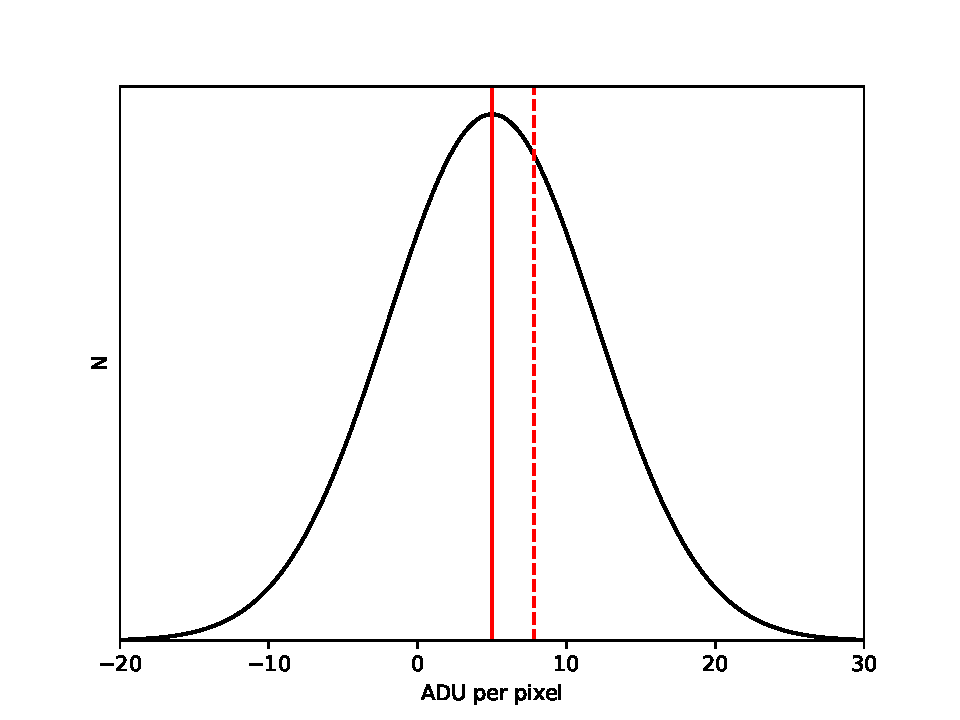
\includegraphics[width=0.7\textwidth]{figures/observations/bias_frame_histogram.pdf}
    \caption{Illustrating the effect of omitting negative values on the average of a distribution. The black line is a Gaussian distribution with an average of 5 and a standard deviation of 7. The vertical dashed line shows the `true' average of 5 ADU, and the vertical red line shows the average given by an ADC that reports negative electron counts as 0.}
    \label{fig:observations:bias frame histogram}
\end{figure}
The readout electronics of a CCD are not perfect, and contribute a small amount of gaussian noise to each pixel called readout noise. The ADC is only capable of recording {\it positive integer values}, and functionally discards negative pixel counts. To illustrate why this is an issue, take the exaggerated example of a readout noise of $7 e^-/{\rm px}$ on a region of the CCD that is stimulated by $5 e^-/{\rm px}$. If negative values are limited to 0, the effect is to increase the average, and Figure~\ref{fig:observations:bias frame histogram} illustrates the effect of discarding negative counts.
This will have a small corrupting effect on low-signal areas of the CCD, crucially the sky background signal.

To prevent corruption, a small bias voltage is applied to each pixel, raising the `floor' away from zero and preventing noise from giving negative readings. To then remove this bias voltage from observations, zero second exposures of a masked detector are taken to characterise the bias voltage for each pixel, and are subtracted off each subsequent exposure. These are known as bias frames, and because the structure of the bias is subtly altered by different instrument setups, a new bias frame is taken when instrument options such as binning pixels together when reading them out, or only reading out partial images, are altered. 


\subsubsection{Flat fielding}

The response of each pixel to photons is similar, but not exactly equal. In addition, the optics of the telescope are not perfect and throughput varies across the field of view, a.k.a vignetting. Dust and imperfections in the optics can also introduce variation across the image. These effects mean that each exposure the instrument takes is convolved with a flat-field response pattern.

In order to characterise the flat-field pattern, an exposure is taken of a known uniform brightness, for example a specialised light box with a high degree of uniformity. 
However, a simpler approach is to observe the sky during sunset, when the sky is still bright and the contribution of light from stars is largely negligible. In the absence of cloud, the twilight sky forms a highly uniform field.
Residual stellar light should still be removed though, so to completely eliminate stars from the flat field observation many exposures are taken while the telescope is nudged by a small amount every few seconds. Then, since the stars move between each exposure, calculating the median frame will effectively remove stars from the image, leaving behind only the uniform sky observation imprinted with the flat-field response pattern. The flat field images are bias corrected to give the final flat image.
Now, by dividing each subsequent exposure by the flat image, we can remove this pattern from future images. 


\subsubsection{Aperture photometry}

While stars are theoretically point sources, we observe them through the atmosphere and the optics of the telescope, which acts to spread the light from a star by $\sim 1-3$ arcseconds. As such, to find the total flux of a star we must sum the contributions to flux from all pixels containing flux, and the HiPERCAM pipeline has two methods for this: `normal' extraction and `optimal' extraction.

Under normal extraction, the user specifies one or more `reference' stars, and one or more `target' stars. The pixel ADU counts around the reference stars are plotted as a function of their radial distance to the peak flux, and the flux distribution is fitted with a Gaussian or Moffat profile. The Full-Width at Half Maximum (FWHM) of this distribution fit is calculated, and all pixels within $x \times \mathrm{FWHM}$ of the peak flux are simply summed to give the extracted flux of a source, cutting off some amount of the wings of the flux distribution. Here, $x$ is a user-defined parameter and while in theory a large value of $x$ would be desirable to capture all flux from a source, adding extra pixels contributes to the readout noise of the detection, and suffers from diminishing returns due to the small amounts of flux contained in the wings.
Also, as the same fraction of light from each source should be lost from both the target sources and reference sources, cutting out these wings should not alter the flux ratio between the sources, and the flux ratio is the relevant quantity under relative photometry.

In many cases, it is preferable to use the `optimal' extraction method, described by \citet{naylor1998}. Here, a weight is taken into account when summing the flux contributions of each pixel based on the {\it expected} contribution to the overall flux. This can give an improvement of $\sim 10\%$ to the signal-to-noise ratio, especially in faint sources as this approach is more robust against poor profile fits. Source profiles often diverge from the idealised Gaussian or Moffat profiles due to noise, or inconsistencies in seeing conditions and telescope guiding, and these effects are more pronounced in fainter sources. 

Finally, the sky background is not perfectly black and must be subtracted from the extracted flux of the sources. This is done by taking an annulus about each source, and assuming it is solely make up of sky background signal. The inner edge of the annulus is selected to be far enough from the source that none of the target's signal is present, and the size of the outer edge is limited by contamination by other sources, and by very large annuli starting to become sensitive to sky variations across the image. The sky signal is then subtracted to isolate the source flux in question.


\section{Photometric calibration}
\label{sect:photometric extraction and calibration}

A comparison star in the same frame as the target was used to account for transparency variations, and standard stars from \citet{smith2002} were used to transform the lightcurves from ADU to the SDSS $u'g'r'i'z'$ photometric system. At the core of the photometric calibrations is the following expression of the apparent magnitude in some band, $m_{app}$, of a target,
\begin{equation}
    \label{eqn:observations:instrumental magnitude from scratch}
    m_{app} = m_{inst} + \chi k_{ext} + m_{zp} + C_{inst}c_{m}
\end{equation}
where $m_{inst}$ is the instrumental magnitude, $-2.5 \rm log(ADU)$, $\chi$ is the airmass of the observation and $k_{ext}$ is the atmospheric extinction coefficient in the relevant band. $m_{zp}$ is the zero point offset of the instrument, calculated from photometric standard stars, ideally taken on the night of an observation. $c_{m}$ is the colour term correction between the response curve of the instrument, and the target photometric system, and $C_{inst}$ is a diagnostic instrumental colour. Each of these terms must be properly handled, and are discussed in turn. 


\subsection{Calculating atmospheric extinction coefficients}
\label{sect:calcualting atmospheric extinction}

Atmospheric extinction was calculated using the longest continuous observation available within a reasonable time from target observations.
The atmospheric extinction values are reported in Table~\ref{table:atmos_extinction}\todo{Currently, this is only for a very narrow range of the actual observations. Generalise this table to include all instruments and locations.}.

To calculate the atmospheric extinction coefficients, aperture photometery was extracted for five sources in these long observations, and the instrumental magnitude, $m_{\rm inst}$, vs airmass, $\chi$, was fit with a straight line for each source. 
The gradients of these lines are the atmospheric extinction coefficients, $k_{\rm ext}$, for the relevant band, and the y-intercept is the instrumental magnitude of that object above the atmosphere, $m_{\rm inst,0}$:
\begin{align*}
    m_{\rm inst} =& m_{\rm inst,0} + \chi k_{\rm ext} 
\end{align*}

\begin{table}
    \centering
    \caption{Typical atmospheric extinction coefficients for La Silla, derived from ULTRACAM/NTT observations.}
    \label{table:atmos_extinction}
    \begin{tabular}{cccc}
        \hline
        Date of Observation & Airmass Range & Band & $k_{ext}$ \\
        \hline
        \hline
        14 Oct 2018   & 1.30-1.98 & $u_{\rm reg}$ & $0.4476$ \\
                      &           & $g_{\rm reg}$ & $0.1776$ \\
                      &           & $r_{\rm reg}$ & $0.0861$ \\
        \hline
        30 Sept 2019  & 1.03-1.63 & $u_{\rm sup}$ & $0.4867$ \\
                      &           & $g_{\rm sup}$ & $0.1803$ \\
                      &           & $r_{\rm sup}$ & $0.0713$ \\
        \hline
    \end{tabular}
\end{table}


\subsection{Transformations between filter systems}
\label{sect:observations:colour correction method}

ULTRACAM and HiPERCAM use an SDSS-\emph{like} filter system with higher efficiency bandpasses, referred to as Super SDSS. There are three relevant photometric paths:
\begin{itemize}
\item SDSS filters, $u', g', r', i', z'$;
\item ULTRACAM/ULTRASPEC SDSS-like, $u_{\rm reg}, g_{\rm reg}, r_{\rm reg}, i_{\rm reg}, z_{\rm reg}$;
\item HiPERCAM/ULTRACAM Super SDSS, $u_{\rm sup}, g_{\rm sup}, r_{\rm sup}, i_{\rm sup}, z_{\rm sup}$.
\end{itemize}

Note that we have no $z$ band observations, so the $z$ band is omitted hereafter.
We aim to place our photometery in the SDSS $u'g'r'i'$ system, as this is the system later used by the white dwarf atmospheric models. The $u_{\rm reg}, g_{\rm reg}, r_{\rm reg}, i_{\rm reg}$\ filters were sufficiently similar to standard SDSS filters that the uncorrected magnitudes of standard reference stars from \citet{smith2002} could be used to calibrate absolute photometery without issue. However, with the new filters, there was concern that the different shape of the sensitivity curve, particularly in the $u'$\ band, differ enough from the standard filters to cause issues with our photometric calibration. Figure~\ref{fig:sdss vs super filters}illustrates the change in throughput between the SDSS photometric system, and the Super SDSS filters, on ULTRACAM on the NTT. 
\begin{figure}
    \centering
    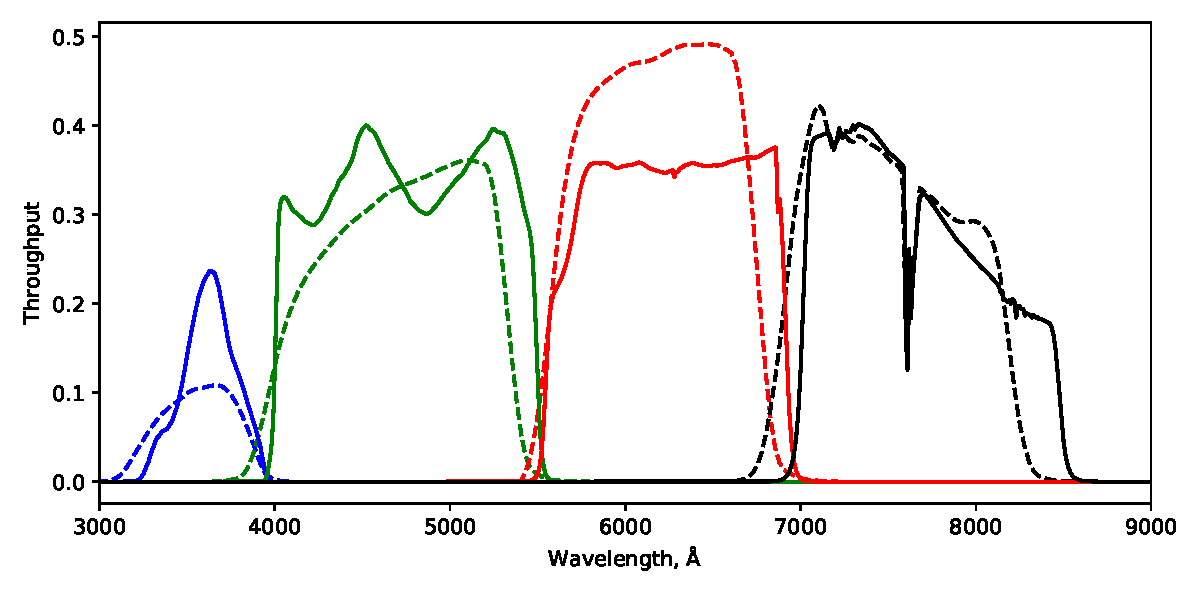
\includegraphics[width=\columnwidth]{figures/three_cvs_with_weird_colours/GeneralFigs/bandpass_diffs_SDSS_dots_UCAMNTT_solid.pdf}
    \caption{The differences in photometric throughput for SDSS filter system (dotted lines), and ULTRACAM Super SDSS filters, for ULTRACAM mounted on the NTT (solid lines). Blue: $u$ bands, Green: $g$ bands, Red: $r$ bands, Black: $i$ bands. Both throughputs include atmospheric extinction of $\chi = 1.3$.}
    \label{fig:sdss vs super filters}
\end{figure}

To perform the colour corrections, the following equation for the magnitude of a star was used, using the $g'$\ band as an example:
\begin{equation}
    \label{eqn:gen magnitudes}
    g' = g_{\rm inst} + \chi k_{\rm ext} + g_{\rm zp} + c_{\rm g, sup}(g'-r') 
\end{equation}
where $g_{\rm zp}$\ is the zero point, $g_{\rm inst} = -2.5 \rm log(ADU/{\it t}_{\rm exp})$
for an exposure time of $t_{\rm exp}$, and $c_{\rm g, sup}$\ is the colour term correction gradient. In theory, the atmospheric extinction term also has some colour dependency, as extinction varies with wavelength. However, the effect is negligible between these photometric systems, so it is omitted.

The optical path of each system was simulated using the \texttt{pysynphot} package, with measured throughputs of all ULTRACAM and HiPERCAM components in the optical path. Models from \citet{Dotter2016} and \citet{Choi2016} were used to generate the \teff\ and \logg\ values of an $8.5$\ Gyr isochrone for main sequence stars with masses from 0.1 to 3 $M_\odot$, spanning from \logg $= 3.73 \to 5.17$, and $\rm{T_{eff}} = 2900K \to 10,300K$. The Phoenix model atmospheres \citep{allard2012} were used to generate model spectra of each mass, which was then folded through each optical path to calculate an AB magnitude. In addition, white dwarf models with \logg$=8.5$\ were similarly processed \citep{koester2010, tremblay2009}, to asses the impact of the different spectral shape on the resulting colour terms.

We synthesised the colour terms between the SDSS and Super SDSS systems, e.g., $g'-g_{\rm sup}$, on ULTRACAM and HiPERCAM for each model atmosphere. These data were plotted against SDSS colours, i.e. $(u'-g')$, $(g'-r')$, $(g'-i')$, and a straight line was fit to the colour relationship. In the example case of $g'-g_{\rm sup}$, this would be
\begin{align*}
    g' &= g_{\rm sup} + g_{\rm zp} + c_{\rm g, sup}(g'-r') \\
    % g' - g_{\rm sup} &= g_{\rm zp} + c_{\rm g, sup}(g'-r')
\end{align*}
These relationships are shown for HiPERCAM in Figure~\ref{fig:observations:ULTRACAM colour corrections} for all four Super SDSS filters used to observe these CVs, and Table~\ref{table:observations:all ULTRACAM colour corrections} and Table~\ref{table:observations:all HiPERCAM colour corrections} contain the coefficients of each colour term correction for both HiPERCAM and ULTRACAM.
$(u'-g')$\ was used to correct $u$\ magnitudes, $(g'-r')$\ was used to correct $g$\ and $r$\ magnitudes, $(g'-i')$\ was used to correct the $i$\ band.
These colour corrections are not generally the same for main sequence stars and white dwarfs, though the colours of the white dwarfs presented in this work are all such that the discrepancy is on the order of a few percent, and is considered negligible.

\noindent\begin{minipage}{\linewidth}
    \centering
    
    \captionof{table}{ULTRACAM colour term best fit lines from Figure~\ref{fig:observations:ULTRACAM colour corrections}. The data are modelled by equations of the form $(u'-u_{\rm sup}) = \phi + c_u(u'-g')$, with $c_u$\ being the relevant colour gradient.}
    \label{table:observations:all ULTRACAM colour corrections}
    \begin{tabular}{cccc}
        Correction          & Diagnostic    & $\phi$    & $c$ \\
        \hline
        \hline
        $(u'-u_{\rm sup})$  &  $(u'-g')$    & 0.003     & 0.036 \\
                            &  $(g'-r')$    & 0.033     & 0.063 \\
                            &  $(g'-i')$    & 0.038     & 0.044 \\
        \hline
        $(g'-g_{\rm sup})$  &  $(u'-g')$    & -0.001    & 0.014 \\
                            &  $(g'-r')$    & 0.010     & 0.027 \\
                            &  $(g'-i')$    & 0.012     & 0.018 \\
        \hline
        $(r'-r_{\rm sup})$  &  $(u'-g')$    & -0.017    & 0.016 \\
                            &  $(g'-r')$    & -0.004    & 0.032 \\
                            &  $(g'-i')$    & -0.002    & 0.022 \\
        \hline
        $(i'-i_{\rm sup})$  &  $(u'-g')$    & -0.031    & 0.020 \\
                            &  $(g'-r')$    & -0.015    & 0.040 \\
                            &  $(g'-i')$    & -0.012    & 0.028 \\
        \hline
        \hline
    \end{tabular}

    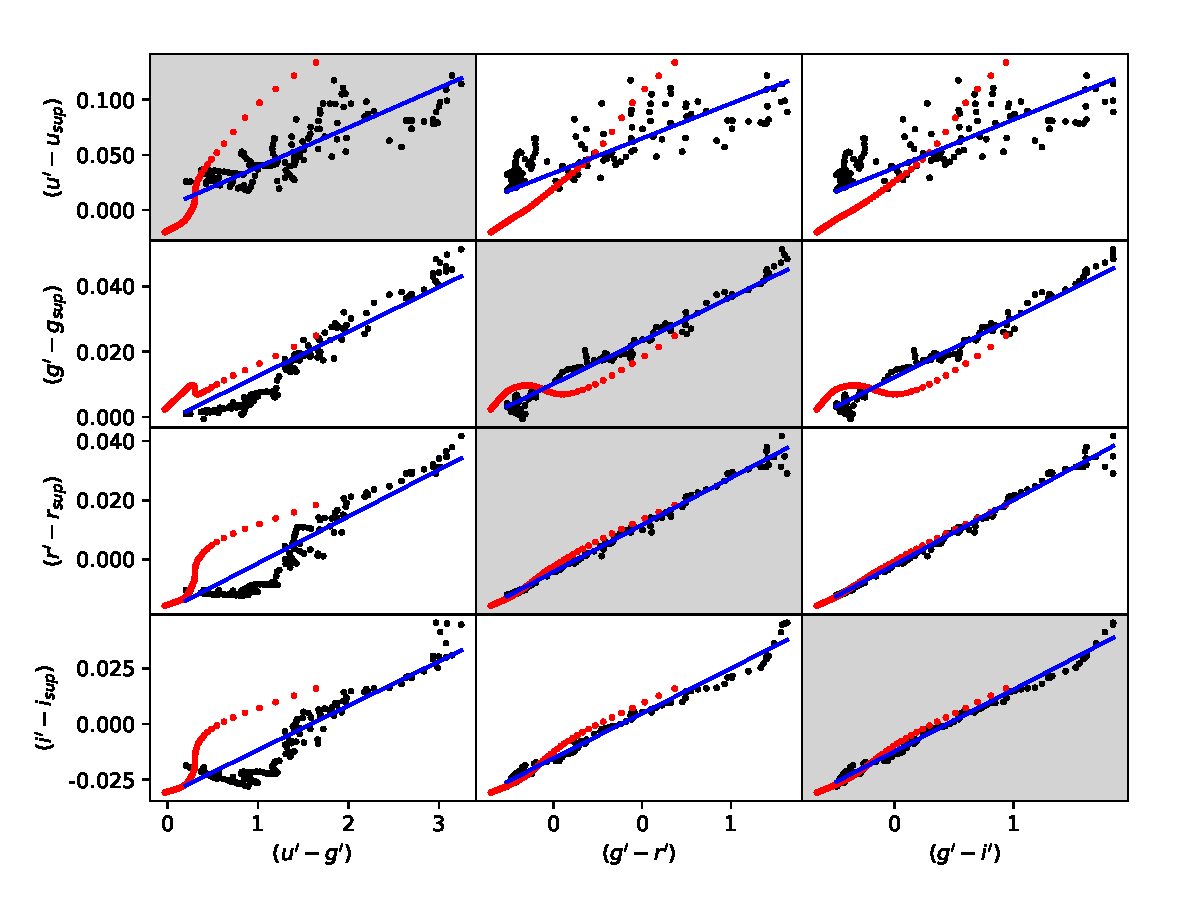
\includegraphics[width=\textwidth]{figures/observations/colour_term_tracks_UCAM.pdf}
    \captionof{figure}{The difference between the classic SDSS photometric system, and the ULTRACAM SuperSDSS filters on the NTT, as a function of SDSS colours, are calculated for model atmospheres. Red points are Koester white dwarf models, black points are Phoenix main sequence model atmospheres, and the blue line is the best fit straight line to both datasets. When applying colour corrections, the highlighted relations were used.}
    \label{fig:observations:ULTRACAM colour corrections}
\end{minipage}

\noindent\begin{minipage}{\linewidth}
    \centering
    
    \captionof{table}{HiPERCAM colour term best fit lines from Figure~\ref{fig:observations:HiPERCAM colour corrections}. The data are modelled by equations of the form $(u'-u_{\rm sup}) = \phi + c_u(u'-g')$, with $c_u$\ being the relevant colour gradient.}
    \label{table:observations:all HiPERCAM colour corrections}
    \begin{tabular}{cccc}
            Correction          & Diagnostic & $\phi$   & $c$ \\
            \hline
            \hline
            $u'-u_{\rm sup}$    & $(u'-g')$   &   0.096   & 0.054\\
                                & $(g'-r')$   &   0.150   & 0.029\\
                                & $(g'-i')$   &   0.152   & 0.022\\
            \hline
            $g'-g_{\rm sup}$    & $(u'-g')$   &   0.008   & 0.023\\
                                & $(g'-r')$   &   0.010   & 0.045\\
                                & $(g'-i')$   &   0.014   & 0.031\\
            \hline
            $r'-r_{\rm sup}$    & $(u'-g')$   &   0.000   & 0.001\\
                                & $(g'-r')$   &   0.001   & 0.003\\
                                & $(g'-i')$   &   0.001   & 0.002\\
            \hline
            $i'-i_{\rm sup}$    & $(u'-g')$   &   0.033   & 0.022\\
                                & $(g'-r')$   &   0.016   & 0.044\\
                                & $(g'-i')$   &   0.012   & 0.030\\
            \hline
            \hline
    \end{tabular}
    
    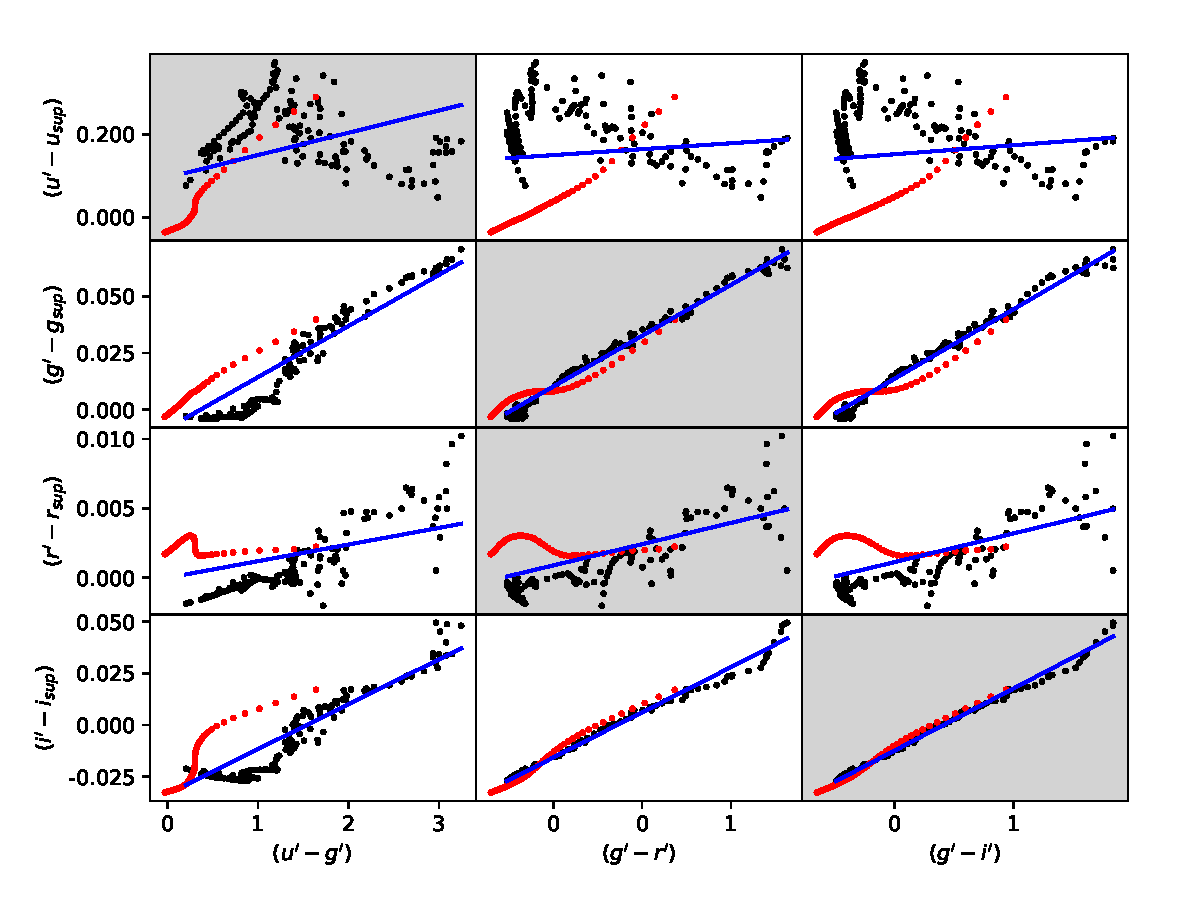
\includegraphics[width=\textwidth]{figures/observations/colour_term_tracks_HCAM.pdf}
    \captionof{figure}{As Figure~\ref{fig:observations:ULTRACAM colour corrections}}
    \label{fig:observations:HiPERCAM colour corrections}
\end{minipage}


\subsection{Calculating comparison star magnitudes}
\label{sect:comparison star mag calc}

Equation \ref{eqn:gen magnitudes} was used to calculate the zero points in each band from the standard star, for the SDSS photometric system.
The comparison star SDSS magnitudes are then determined. As the colour term corrections are dependent on SDSS colours, an iterative approach was used to converge on these values. The SDSS magnitudes are related to the instrumental magnitudes by:
\begin{align*}
    u' =& u_{\rm inst,0} + u_{\rm zp} + c_{\rm u, sup}(u' - g') \\
    g' =& g_{\rm inst,0} + g_{\rm zp} + c_{\rm g, sup}(g' - r') \\
    r' =& r_{\rm inst,0} + r_{\rm zp} + c_{\rm r, sup}(g' - r') \\
    i' =& i_{\rm inst,0} + i_{\rm zp} + c_{\rm i, sup}(g' - i') \\
\end{align*}
Initially, $u',g',r',i'$\ magnitudes are set equal to the instrumental magnitudes, and a new set of $u',g',r',i'$\ magnitudes are calculated. The new values are then used to repeat the calculation until a new iteration produces no change, typically after $\sim$4 loops.


\subsection{Producing a flux-calibrated target lightcurve}
\label{sect:flux calibrating the lightcurve}

Finally, the target lightcurves can be calculated. We need to both correct the target star lightcurve for transparency variations, and convert from counts to calibrated fluxes. As we are producing a flux-calibrated lightcurve in the SDSS photometric system using a significantly different photometric system, the simple ADU ratio between the target and comparison is insufficient. Consider the target star $g'$ magnitude and flux, $g^t, F^t$, and comparison star $g'$ magnitude and flux, $g^c, F^c$:
\begin{align*}
    g^t =& g^t_{\rm inst,0} + g_{\rm zp} + c_{\rm g, sup}(g'-r')^t \\
    g^c =& g^c_{\rm inst,0} + g_{\rm zp} + c_{\rm g, sup}(g'-r')^c \\
\end{align*}
since,
\begin{equation*}
    g^t - g^c = -2.5{\rm log}\Big(\frac{F^t}{F^c}\Big) \\
\end{equation*}
we can write
\begin{align*}
    % g^t - g^c =& g^t_{\rm inst,0} - g^c_{\rm inst,0} + c_{\rm g, sup}\big((g-r)^t - (g-r)^c\big) \\
    \frac{F^t}{F^c} =& 10^{-0.4(g^t_{\rm inst,0} - g^c_{\rm inst,0})} \cdot 10^{-0.4c_{\rm g, sup}\big((g'-r')^t - (g'-r')^c\big)} \\
    % \frac{F^t}{F^c} =& \frac{ADU^t/s}{ADU^c/s}\cdot 10^{c_{\rm g, sup}\big((g-r)^t - (g-r)^c\big)} \\
    \frac{F^t}{F^c} =& \frac{ADU^t}{ADU^c}\cdot K^{t,c} \\
\end{align*}
where $K^{t,c} = 10^{-0.4c_{\rm g, sup}\big((g'-r')^t - (g'-r')^c\big)}$.
This accounts for differences in wavelength response between the two systems when calculating the flux ratio, and is applied to each frame. The $(g'-r')^t$\ magnitudes are calculated using a sigma-clipped mean instrumental magnitudes computed from all frames in the observation. In practice, the factor $K^{t,c}$\ varies from $\sim 1.0 - 1.1$\ for our observations. 

While developing this correction method, some verification tests were performed.
ASASSN-16kr was observed in both the standard SDSS filters in 2018, and the super SDSS filters in 2019. This presented an opportunity to compare the corrected 2019 data with the fluxes observed in 2018. Additionally, both ASASSN-16kr and SSSJ0522-3505 use multiple standard stars across observations, which should agree if the calibration has been done correctly. In all cases, the flux-calibrated lightcurves were similar and the white dwarf colours consistent, suggesting that this method of flux calibration is indeed accurate.

We add a 3\% systematic error in quadrature to the white dwarf fluxes when fitting for the effective temperature. This is a practice established by \citet{McAllister2019}, to account for possible systematic error in flux calibration and modelling.


\section{Catalogue of observations}

\todo{Make a Table of observations.}The observations analysed in this work span the full decade from 2011, through to 2021, and have been taken from multiple sites as the instruments move from telescope to telescope. To aid with the readability, a key is provided in Table~\ref{tab:observation acronyms} of the acronyms used for instruments and telescopes. 

\begin{table}
    \centering
    \begin{tabular}{c|c}
        Acronym & Expansion \\
        \hline
        NTT & New Technology Telescope \\
        GTC & Gran Telescopio Canarias \\
        TNT & Thai National Telescope \\
        WHT & William Herschel Telescope \\
        VLT & Very Large Telescope \\ 
        HCAM & HiPERCAM \\
        UCAM & ULTRACAM \\
        USPEC & ULTRASPEC \\
    \end{tabular}
    \caption{Acronyms used in the observation summaries.}
    \label{tab:observation acronyms}
\end{table}


\chapter{Modelling techniques and methodology}
\lhead{\emph{Methods}} % This is for the header on each page - perhaps a shortened title
\label{chpt:modelling and techniques}

This chapter describes in detail the two modelling techniques used for this thesis: the characterisation of a CV using multi-band eclipse modelling, and using MESA models to infer the long-term mass loss rate of a system from its donor properties.
Since the models used in this analysis are computationally expensive and require large parameter spaces, the choice of fitting algorithm is important. The majority of the parameter optimisation done in this work uses a type of Markhov Chain Monte Carlo (MCMC) technique, and this is described in detail in \S\ref{sect:modelling:parameter optimisation of many variables}, before discussing the models themselves.


\section{Parameter optimisation of many variables}
\label{sect:modelling:parameter optimisation of many variables}
Frequently in science, a model must have its input parameters fit to data. For models with few input parameters and well-behaved evaluation metrics (i.e. goodness-of-fit varies smoothly with input parameters), optimisation is relatively easy, but this is often not the case; for example the eclipse modelling portion of this work (\S\ref{sect:modelling:eclipse modelling}) has 18 parameters for a single eclipse, and fitting a full dataset frequently involves fitting  100+ parameters. To make matters worse, the eclipse model is fairly expensive to compute in large numbers, making a full exploration of the parameter space impractical.

The MCMC method is now a well-established tool in astronomy. It is robust, efficient when used properly, and yields the probability distribution of the variables being optimised even when the distributions are not well-described by simple functions. This has led to MCMC often being the method of choice when fitting models.
This section provides a working knowledge of MCMC, but for an in-depth introduction and review of the technique and its various sub-types see \citet{sharma2017}.


\subsection{Bayesian analysis}
\label{sect:modelling:Bayesian analysis}
Bayesian inference uses known, `prior' knowledge combined with new information, `data', to derive a better understanding - the `posterior' knowledge - of a model. This somewhat self-evident intuition is formalised as Bayes' Theorem, which calculates the posterior probability, $p(\theta | D, I)$ a set of model parameters, $\theta$, given some observed data, $D$, and background information, $I$.
\begin{equation}
    \label{eqn:modelling:bayes symbolic}
    p(\theta | D,I) = \frac{\mathcal{L}(D | \theta, I) \cdot q(\theta | I)}{p(D|I)}
\end{equation}
Here, $\mathcal{L}(D | \theta, I)$ is the probability of the observed data, given a model and prior information, so is called the likelihood of the data.
$q(\theta|I)$ is the probability of the model being valid, given some prior information, so is called the prior distribution. Finally, $p(D | I)$, or the probability of observing the data, given the previously known information, is also called the `Evidence', and acts as a normalisation factor. Using this vocabulary, Equation~\ref{eqn:modelling:bayes symbolic} can be written as:
\begin{equation}
    \label{eqn:modelling:bayes english}
    \rm Posterior = \frac{Likelihood \times Prior}{Evidence}
\end{equation}
In Bayesian inference, the goal is to find the posterior distribution of the parameters of a model, given some data and any prior information.


\subsection{MCMC optimisation}
\label{sect:modelling:affine invariant MCMC}
The MCMC technique is a class of tools developed to approximate the posterior distribution in Equation~\ref{eqn:modelling:bayes symbolic}. Analytical calculations of the posterior are predicated on knowing the analytical forms of the likelihood, prior and evidence, which is often not known.

An MCMC sampler, as the name suggests, is a combination of a Monte Carlo method, a class of algorithms that rely on random sampling to find a result, and a Markov chain, a mathematical system that transitions between states according to probabilistic rules \citep{foreman2012}.
An MCMC randomly samples the prior distributions of the model variables (the Monte Carlo half of the algorithm), evaluates their $\mathcal{L}$ and $q$, and either accepts them onto its chain of sampled points or not, depending on if they meet a set of conditions (the Markov chain half of the algorithm). If the $\mathcal{L}$ of the proposed set of variables is higher than the $\mathcal{L}$ of the last set on the chain, the proposed set of variables is accepted. If $\mathcal{L}$ is lower, the algorithm randomly accepts or rejects the proposed step.
Conveniently, $\mathcal{L}$ is usually related to the $\chi^2$ metric by $\mathcal{L} \propto \mathrm{exp}(-\chi^2/2)$, so a change in $\mathcal{L}$ is often relatively easy to compute.
The method by which a new set of parameters is proposed, and acceptance decided in the event of a decrease in $\mathcal{L}$ is the sampling method, and several choices exist for different types of problems. The sampling method used here is the affine invariant sampling method with parallel tempering, described below.

By giving a finite chance to accept a `worse' set of parameters, the chain is, in theory, allowed to explore and sample the entire possible parameter space without becoming trapped in local minima, though this requires an infinitely long chain.
However, as the sampler preferentially accepts positions with higher $\mathcal{L}$, as the length of the chain increases the distribution of samples on the MCMC chain approaches the `true' distribution of the posterior.


\subsubsection{Affine invariant ensemble sampling}
\label{sect:modelling:Affine invariant ensemble sampling}
The affine invariant ensemble method of sampling was developed by \citet{goodman2010}, and makes use of many `walkers' sampling the parameter space in tandem.
Each walker functions as an individual MCMC chain, and the walkers interact by proposing steps based on the current states of other walkers.
A new parameter vector for walker $k$ is proposed via a `stretch move'; another walker, $j$ is chosen at random, and the last position vectors on each chain, $\theta_{j,N}$ and $\theta_{k,N}$, are used to propose a new position, $\Theta_k$, that lies somewhere on the line connecting the two position vectors.
\begin{equation}
    \Theta_k = \theta_j + z \cdot (\theta_k - \theta_j)
\end{equation}
The variable $z$ determines the location of the new vector on the line, and is randomly drawn from a probability distribution $g(z)$,
\begin{equation}
    g(z) \propto
    \begin{cases}
        \frac{1}{\sqrt{z}}, & \frac{1}{2} \le z \le 2 \\
        0, & Otherwise
    \end{cases}
\end{equation}
The choice of $g(z)$ favours a consolidation of the walkers, and aids convergence on regions of high $\mathcal{L}$. A schematic of this stretch move concept is shown in Figure~\ref{fig:modelling:stretch move}.
\begin{figure}
    \centering
    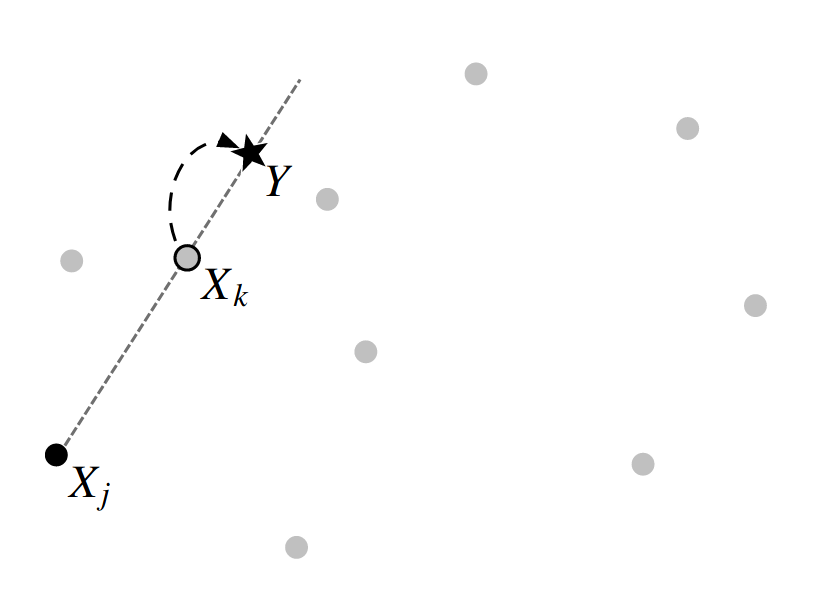
\includegraphics[width=.7\textwidth]{figures/modelling/stretch_move.png}
    \caption{Reproduced from \citet{goodman2010}, showing the concept of a stretch move proposal. The proposed next step for $j$ is given by choosing a random position on the line joining the last step on chain $j$, $X_j$, and the last chain on another walker chosen at random, $X_k$. The proposed step is shown by the star, $Y$. Grey dots with no outlines illustrate the other walkers in the ensemble, but are unused.}
\label{fig:modelling:stretch move}
\end{figure}

Then, $\Theta_k$ is either accepted or rejected from the chain depending on the current state of the chain. Recall that if the proposed $\mathcal{L}_{N+1} > \mathcal{L}_{N}$, i.e. the likelihood has improved, the sample is immediately accepted. However, if $\mathcal{L}_{N+1} < \mathcal{L}_{N}$, the acceptance is determined by the transition probability, $P(\Theta_k | \theta_{k,N})$, defined as
\begin{equation}
    P(\Theta_k | \theta_{k,N}) = \alpha(\Theta_k | \theta_{k,N}) \cdot q(\Theta_k | \theta_{k,N})
\end{equation}
where $\alpha(\Theta_k | \theta_{k,N})$ is the acceptance probability,
\begin{equation}
    \alpha(\Theta_k | \theta_{k,N}) = \mathrm{min}\bigg( 1,\ z^{n-1}\frac{\mathcal{L}(\Theta_k)}{\mathcal{L}(\theta_{k,N})} \bigg)
\end{equation}
for a model with $n$ dimensions.
A random number, $u$, is drawn from a uniform distribution from 0 to 1, and if $u < \alpha(\Theta_k | \theta_{k,N})$, the proposed position is accepted.
This quantifies two aspects of the sampler: the larger the drop in the probability that a new $\Theta_k$ describes observation, the \textit{less likely} the algorithm is to accept $\Theta_k$ onto the chain; and larger stretch moves are more likely to be accepted.
At each step in the MCMC, every walker has a new position proposed this way.

% This finite chance to accept a new point, even if it is less likely to describe the data, makes the chain \textit{reversible} and allows the algorithm to explore the full allowable parameter space (given an infinite number of steps) even if doing so first requires moving to a less preferred $\theta$.
The affine invariant ensemble sampler benefits significantly from having the walkers in the ensemble interact, as they can communicate to other walkers regions of high $\mathcal{L}$ even between walkers in different local minima. Further, the sampler has a higher likelihood to accept dispersing steps than consolidating steps, so walkers are only likely to gather in deep minima, increasing exploration except in the case of a significantly higher likelihood.
This improves the ensemble's ability to both locate the global minimum, and to sample non-spherical probability distributions (a task that can be difficult for simpler sampling techniques).
Further, this algorithm is able to have the proposal and evaluation of new steps in every chain performed \textit{simultaneously}, significantly improving computation time;
a typical rule-of-thumb is to use $2n$ walkers for $n$ parameters being optimised \citet{goodman2010}, and since the number of walkers is almost always larger than the number of available threads, increased evaluation time scales well with more threaded computation.


\subsubsection{Parallel tempering}
\label{sect:modelling:parallel tempering}

Parallel tempering is an additional element of an MCMC sampler that helps in more fully exploring the parameter space in more complex models, while also being more capable of characterising posterior distributions in the case of complex correlations between parameters.

In metallurgy, a metal can be toughened by relieving its internal stresses through tempering, a treatment in which a metal is first heated to a high temperature, then slowly cooled.
While the metal is at a high temperature, impurities are able to diffuse throughout the crystal structure of the metal and explore possible crystallisation locations. As the metal slowly cools, impurity atoms are gradually more and more attracted to areas of the crystal that exert less stress on the material, until the metal is fully cooled and the majority of atoms have found areas of local minima in stress potential.

The ensemble MCMC can take analogy from this `hot' exploration phase and `cool' settling phase\todo{I need a reference for parallel tempering...}. This is done by running several parallel ensembles, that each have a different `temperature' between 1 and $\infty$. Each ensemble samples a modified posterior, that follows $\pi_T(\Theta)$;
\begin{equation}
    \pi_T(\Theta) = [\mathcal{L}(\Theta)^\frac{1}{T}] q(\Theta)
\end{equation}
As $T \rightarrow \infty$, the chain samples the prior with no respect to how well $\Theta$ describes the data. This hot chain is analogous to the diffusive atoms with much higher thermal energy than the stress potential of the metal, and is free to randomly explore available parameter space without being restricted by the $\mathcal{L}$ function, potentially finding regions of high likelihood far from the initial conditions and communicating these regions back to cooler ensembles. Cooler temperatures are analogous to the cooling metal -- drawn increasingly strongly towards regions of high likelihood.
The cold case of $T \equiv 1$ behaves equivalently to a normal ensemble sampler.

Note that because hotter walkers are less sensitive to $\mathcal{L}$, their posterior no longer accurately reflects the `true' distribution. If a parameter is described by a Gaussian distribution with a standard deviation, $\sigma$, the tempered $\mathcal{L}$ will have a standard deviation of $\sigma \sqrt{T}$.

When running a parallel tempered MCMC, the values used in the software are $\beta = 1/T$, for which we choose between 3 and 5 evenly spaced values of $\beta$ between 0 and 1.
The number of temperatures used depends on the evaluation time; since parallel tempering runs multiple full ensembles in tandem, in models with very large numbers of parameters it becomes highly desirable to use as few temperatures as possible. However, the penalty in computation time per step comes with the benefit of a dramatically improved ability to locate the global minimum, especially in complex parameter space.

\subsection{The binary chop}

When searching for the root of a simple model, i.e. one with a single input parameter, $x$, and a single output metric, $y$, that either monotonically increases or decreases with $x$, we use the binary chop algorithm.
This requires relatively few evaluations to find the root of a function, i.e. $y(x_0) = 0$.
If two values of $y$ are known to have opposite signs, e.g. $y_1(x_1)$ is positive and $y_2(x_2)$ is negative, it can be deduced that $x_0$ lies between $x_1$ and $x_2$. Then, by repeatedly evaluating midpoint between the two values of $x$ known to be closest to $x_0$, the algorithm will tend towards $x_1 \sim x_2 \sim x_0$. In practice, the optimisation terminates when $y(x_1) - y(x_2)$ is within some tolerance.
Step-by-step, this proceeds as follows:
\begin{enumerate}
    \setlength\itemsep{0em}
    \item First, evaluate the upper and lower limits of $x$, $x_{\rm low}$ and $x_{\rm high}$, to ensure that one returns a negative $y$, and one returns a positive $y$
    \item Evaluate $y(x_{\rm mid})$, where $x_{\rm mid} = 0.5(x_{\rm low} + x_{\rm high})$.
    \item If $x_{\rm low}$ has the same sign as $x_{\rm high}$, assign $x_{\rm high} = x_{\rm mid}$, or vice-versa for $x_{\rm low}$.
    \item Check if the difference between $y(x_{\rm low})$ and $y(x_{\rm high})$ is within tolerance. If it is, terminate the optimisation. Otherwise, repeat the process again.
\end{enumerate}


\section{Finding an orbital ephemeris}
\label{sect:modelling:getting ephemeris}

Crucial to both observing and modelling an eclipse is a good knowledge of the orbital ephemeris. This is described by the equation
\begin{equation}
    \label{eqn:modelling:general ephemeris equation}
    T_{\rm ecl} = T_0 + P_{\rm orb} E
\end{equation}
where $T_{\rm ecl}$ is the time of mid-eclipse, $T_0$ is the mid-eclipse time of the zeroth eclipse, and $E$ is the eclipse number. Accurately calculating $T_{\rm ecl}$ is important to scheduling observations of a system, and $P_{\rm orb}$ is a crucial to the eclipse modelling.

As observations are often separated by several months or even years, an error in $P_{\rm orb}$ of even $\sim 0.1$ seconds can accumulate to give significantly inaccurate predicted eclipse times. This need for precision also requires the definition of {\it where} a time is recorded from, as the delay introduced by the light travel time from one side of the earth's orbit to the other can significantly offset an observed time. All eclipse times presented in this thesis are given in the Barycentric Modified Julian Date (BMJD), which is the time of eclipse as measured from the centre of mass of the solar system. Note that this is different to the heliocentric MJD often seen in the literature, and where heliocentric literature values are used, they are converted to BMJD.
Two timescales are relevant: UTC, in which a clock ticks at the rate of an earth-bound observer; and TDB, in which a clock ticks at the rate of an observer at the barycentre of the solar system. Literature values, and the clocks in the observing cameras, use UTC time. This is converted to TDB during photometric calibration, for consistency with the BMJD times used.

\subsection{Finding eclipse times}
\label{sect:modelling:finding eclipse times}

When finding an eclipse time, simply taking a time of minimum light is insufficient for the systems in this work. This is because it is common for CV eclipses to have very flat eclipse minima, and because CV eclipses have a fairly complex structure.
Rather, finding the mid-eclipse time is done by looking at the numerical derivative of an eclipse.
First, an eclipse is smoothed to remove short term fluctuations, partly those due to noise but also to mitigate the short term flickering often seen in CVs. This initial smoothing is done by applying a median filter to the data. Then, the numerical derivative is calculated and smoothed again, this time with a `boxcar' convolution (a.k.a. a moving average). Properly filtered, the dominant remaining features of the numerical derivative are the ingresses and egresses of the white dwarf and bright spot.
The white dwarf ingress and egress are, in theory, symmetrical -- the ingress should be a sharp, negative spike, and egress should be a sharp, positive spike. As the two should be the same shape, a double-Gaussian is fit to the derivative, using manually chosen initial conditions. In this model, two Gaussians share a width, $\sigma$, and have their mid-points equidistant from a central point. The magnitude of their heights are shared, but with opposite signs;
\begin{align*}
    T_{\rm 1,2} = T_{\rm ecl} \pm \Delta T \\
    h_{\rm 1,2} = \pm h
\end{align*}
where $T_{1,2}$ are the respective midpoints of the two Gaussians, $h_{1,2}$ are their respective heights, and $2\Delta T$ is the distance between the two Gaussians.
The derivative is then fit with these four free parameters ($T_{\rm ecl},\ h,\ \Delta T,\ \sigma$) using an MCMC with wide, uniform priors of appropriate ranges, to give the $T_{\rm ecl}$.

\subsection{Computing period}
\label{sect:modelling:Computing ephemeris}

To find a rough initial ephemeris of a system, at least two eclipse observations with known $E$ are necessary. Given no prior knowledge of $P_{\rm orb}$ and $T_0$, this can be done by simply observing the system for several hours, until two consecutive eclipses are seen. This gives a rough measure of $P_{\rm orb}$, but can be significantly refined with longer baseline observations.
For each observed $T_\mathrm{ecl}$, $E$ could unambiguously be determined, either from observing consecutive eclipses or from previously reported literature values. Where literature values were used to calculate a value of $E$, the result never deviated from an integer by more than 0.25 and were rounded to the nearest whole number.

An MCMC algorithm was used to fit a straight line model to the independent variable $E$\ and dependent variable $T_\mathrm{ecl}$, with a gradient $P$\ and intercept $T_0$; i.e. model values of $T'_{\rm ecl}$ were generated from the set of $E$ and a proposed $(P, T_0)$ pair, and $(T_{\rm ecl} - T'_{\rm ecl})$ was minimised. Again, wide uniform priors were used for $P$ and $T_0$, based on initial values.

The model also accounts for potential systematic differences in timing accuracy between instruments by having variable error scale factors applied to all eclipses observed with a specific instrument. For example, the timing reported for eclipses observed with ULTRACAM may be systematically offset from reality, and the errors associated with those observations might need to be larger than reported to be consistent with data from other instruments. The prior distribution assumed for these error factors was log-uniform ranging from 0.01 to 5, which favours the smallest error-multiplying factor consistent with the data.

Finally, the values of $E$ for each eclipse were offset to minimise the covariance between $T_0$ and $P$.
Consider a predicted eclipse time for $E$. The uncertainty on $T_{\rm ecl}$ in Equation~\ref{eqn:modelling:general ephemeris equation} can be written as,
\begin{equation}
    \label{eqn:modelling:error in ephemeris}
    \sigma_{T{\rm ecl}}^2 = \sigma_{\rm T0}^2 + 2\sigma_{\rm T0} \sigma_{\rm P}E + \sigma_{\rm P}^2 E^2
\end{equation}
from the standard error propagation formula.
To evaluate an alternative set of $E'$, $E$ can be offset by some integer, $N$, with $E' = E - N$. By substituting this into equation~\ref{eqn:modelling:error in ephemeris}, expanding out the brackets, and consolidating some terms, $\sigma_{T{\rm ecl}}^2$ becomes,
\begin{align*}
    \sigma_{T{\rm ecl}}^2 =& \sigma_{\rm T0}^2 + 2\sigma_{\rm T0} \sigma_{\rm P}(E'+N) + \sigma_{\rm P}^2 (E'+N)^2 \\
    % =& (\sigma_{\rm T0}^2 + \sigma_{\rm P}^2 N^2 + 2\sigma_{\rm T0} \sigma_{\rm P} N) + 2(\sigma_{\rm T0} \sigma_{\rm P} + \sigma_{\rm P}^2 N)E' + \sigma_{\rm P}^2 E'^2
\end{align*}

To minimise the cross-correlation between $P$ and $T_0$, the second term of the above equation should be minimised.
This is achieved by setting $N = -(\sigma_{\rm T0}\sigma_{\rm P})/(\sigma_{\rm P}^2)$, and re-fitting the ephemeris. Then, the above becomes:
\begin{equation}
    \sigma_{T{\rm ecl}}^2 = \sigma_{\rm T0}^4 + (\sigma_{\rm P}E')^2
\end{equation}
with no cross correlation, in theory. In practice, as $E$ must be rounded to an integer, some residual cross-correlation persists, but is minimised.

\newpage
\section{Modelling CV eclipse lightcurves}
\label{sect:modelling:lightcurve modelling}

\begin{table}
    \centering
    \caption{The various symbols used in this chapter, and their meanings.}
    \label{table:modelling:parameter key}
    \begin{tabular}{cl}
        \hline
        Symbol & Parameter \\
        \hline
        \hline
        $F_{\rm wd,\ donor,\ disc, bs}$                                 & White dwarf, donor star, disc, and bright spot fluxes   \\
        $T_{\rm eff}$                                                   & White dwarf effective temperature \\
        log($g$)                                                        & White dwarf surface gravity \\
        $M_{\rm wd}$, $R_{\rm wd}$                                      & White dwarf mass and radius                             \\
        $M_{\rm donor}$, $R_{\rm donor}$                                & Donor star mass and radius                              \\
        $q$                                                             & Mass ratio                                              \\
        $a$                                                             & Orbital separation                                      \\
        $x_{l1}$                                                        & Distance from the white dwarf to the $L_1$ point        \\
        $i$                                                             & inclination                                             \\
        $\Delta \phi$                                                   & White dwarf eclipse width in units of phase             \\
        $R_{\rm disc}$                                                  & Accretion disc radius                                   \\
        $b$                                                             & Disc surface profile exponent                           \\
        $\theta_{\rm yaw}$, $\theta_{\rm tilt}$, $\theta_{\rm az}$      & Bright spot yaw, tilt, azimuth                          \\
        $S$                                                             & Bright spot length scale                                \\
        $Y, Z$                                                          & Bright spot profile exponents                           \\
        $u_{\rm ld}$                                                    & White dwarf limb darkening coefficient                  \\
        $\phi_0$                                                        & An eclipse phase offset                                 \\
        $\pi$                                                           & Parallax                                                \\
        E(B-V)                                                          & Interstellar extinction   \\

        \hline
    \end{tabular}
\end{table}

To determine the system parameters for the CVs in this study, the eclipse light-curves were modelled. This method is more frequently applicable in CVs than the more traditional approach of using spectroscopic eclipsing binaries, since the donor star is rarely directly visible. Compared to using the superhump period excess to estimate the mass ratio \citep{patterson2005, knigge2006}, lightcurve modelling requires few assumptions. However, it does require reasonably precise alignment of the system and so is not possible for a large fraction of CVs.

CV eclipse modelling was first developed by \citet{wood1986}, and has been refined significantly over the last decade \citep{Savoury2011, littlefair2014, McAllister2017, McAllister2019}. The method relies on four assumptions, namely that: \textit{(1)} the stream of mass flowing from the donor to the white dwarf follows a ballistic trajectory, \textit{(2)} the white dwarf obeys a theoretical mass-radius relationship, \textit{(3)} the white dwarf is unobscured by the accretion disc or other sources of intra-system material, and \textit{(4)} the donor exactly fills its Roche lobe.
Most of these assumptions are considered robust, though the visibility of the white dwarf been called into question by \citet{Spark2015}.
The white dwarf mass-radius relationship was recently tested by \citet{parsons2017}, and found to be a reasonable assumption.
Assuming that the mass stream following a ballistic trajectory appears to be a reasonable assumption, as the thermal velocity of the donor surface is orders of magnitude lower than the orbital velocity of the two stars.
However, the most convincing argument to the validity of these assumptions are comparative studies, showing good consistency between eclipse modelling and other techniques \citep{tulloch2009,copperwheat2012,savoury2012,sion2022}.

The rough outline of the modelling process is described here, but is detailed fully in \S\ref{sect:modelling:eclipse modelling}. Throughout, symbols are typically used when referring to model and system parameters, and a key is provided in Table~\ref{table:modelling:parameter key}.
Radii are found by assuming that the secondary star completely fills its Roche lobe, which is required for mass transfer and ensures that the donor radius is solely a function of mass ratio, $q$, and orbital separation, $a$, c.f.~Equation~\ref{eqn:introduction:eggleton approximation}.
The white dwarf eclipse width is set by the width of the donor, $a$, inclination, $i$, and $q$ \citep{bailey1979}.

Assuming that the mass stream between the two stars follows a ballistic trajectory puts the stream on a calculable path, determined by $q$ \citep{Lubow1975}. This allows the location of the bright spot to be fixed in space, as the point at which this path intersects the outer edge of the accretion disc. Therefore, the phase of the bright spot ingress and egress is a function of $q$, $i$, $\Delta\phi$, and disc radius.
By assuming that the white dwarf is unobscured, the duration of white dwarf ingress and egress are dependent on the white dwarf radius and inclination.

Four components of the eclipse model are the four component fluxes, $F_{\rm wd}$, $F_{\rm donor}$, $F_{\rm disc}$, $F_{\rm bs}$.
As the white dwarf is assumed to follow a known mass-radius relationship, by fitting the observed white dwarf colours with a temperature, gravity, distance and interstellar extinction, the temperature and radius of the white dwarf yield a mass. The donor mass is then a simple product of the white dwarf mass, and $q$.
The final result of modelling are then the following system parameters:
\begin{itemize}
    \setlength\itemsep{0em}
    \item white dwarf and donor masses
    \item white dwarf and donor radii
    \item orbital separation
    \item orbital velocity of the white dwarf and donor
    \item inclination
    \item white dwarf effective temperature and surface gravity
    \item distance
\end{itemize}

Practically, the modelling actually takes place in two phases, which are each described in detail. First the phase-folded eclipse is modelled under the above assumptions using proxy variables, then the resulting proxy variables are converted to physical parameters once observations are well-described by an eclipse model. This proxy variable fitting is done for the sake of computational efficiency.

Note that this model requires simultaneously fitting many variables simultaneously, thus finding the best-fitting parameters to observed data is complex. The technique used is described in \S\ref{sect:modelling:optimising eclipse model parameters}.

\subsection{Phase-folded eclipse modelling}
\label{sect:modelling:eclipse modelling}

Recall that the light from a CV originates from four distinct objects in the system. The white dwarf and donor star, the accretion disc about the white dwarf, and the bright spot impact region (hereafter simply `the bright spot'), where transferred material impacts the outer rim of the accretion disc and liberates significant amounts of energy. Notably the bright spot emits flux directionally, so beaming must also be accounted for in the model.
The anatomy of a CV eclipse lightcurve is a sequence of five events, that usually occur in the following order:
\begin{enumerate}
    \setlength\itemsep{0em}
    \item a pre-eclipse hump is often seen as the bright spot rotates to point at the observer
    \item The white dwarf becomes obscured by the donor
    \item The bright spot becomes obscured by the donor
    \item The white dwarf emerges from behind the donor
    \item The bright spot emerges from behind the donor
\end{enumerate}
Figure\todo{Make a figure for this} shows a typical lightcurve, with these events marked.

A single eclipse is described by 18 parameters:
\begin{itemize}
    \setlength\itemsep{0em}
    \item White dwarf, donor star, disc, and bright spot fluxes, $F_{\rm wd,\ donor,\ disc, bs}$
    \item Mass ratio, $q$
    \item White dwarf eclipse width in units of phase, $\Delta \phi$
    \item Scaled white dwarf radius, $R_{\rm wd} / x_{l1}$
    \item White dwarf limb darkening coefficient, $u_{\rm ld}$
    \item Scaled outer disc radius, $R_{\rm disc} / x_{l1}$
    \item Disc surface profile exponent, $b$
    \item Seven parameters describing the bright spot
    \item An eclipse phase offset, $\phi_0$
\end{itemize}
The seven bright spot parameters are not physically motivated, but describe a flexible empirical bright spot model designed to capture a large range of bright spot eclipse morphologies.

\subsubsection{The white dwarf}

The white dwarf is modelled as a luminous disc, with a total surface brightness $F_{\rm wd}$ and a radius of $R_{\rm wd} / x_{l1}$. It is subject to limb darkening, using a linear prescription:
\begin{equation}
    \frac{I_l}{I_0} = 1 - u_{\rm ld}(1 - {\rm cos}\beta)
\end{equation}
where $I_0$ is the intensity at the centre of the disc, and $I_l$ is the intensity at a limb. $\beta$ is the angle between the line normal to the surface of the white dwarf, and the observer's line of sight.
However, the observations are not precise enough to constrain $u_{\rm ld}$, so a Gaussian prior derived from the white dwarf $T_{\rm eff}$ and $\log(g)$ is used.

\subsubsection{The donor star}

The secondary star does not become obscured during an eclipse, but there is still some variation in its brightness. The donor is not spherical, so a small ellipsoidal variation is seen as it rotates to expose more or less of its surface to the observer. As a result, the donor is modelled as a limb darkened, and gravity darkened disc with total surface brightness $F_{\rm donor}$, and a modulation to describe the changing observable surface area.

\subsubsection{The accretion disc}

The accretion disc is modelled as a series of annular rings about the white dwarf, extending out to $R_{\rm disc} / x_{l1}$ and with a total surface brightness of $F_{\rm disc}$. The intensity of each annulus decreases with distance from the white dwarf, following an exponential formula, $I_i \propto R^{-b}$ for ring $i$ at distance $R$ from the white dwarf. As $b$ is a free parameter in the model, the disc brightness can be made more or less centrally concentrated to match observations. As the bright spot location is determined by $q$ and $R_{\rm disc} / x_{l1}$, the phases of bright spot ingress and egress provide a valuable constraint for $R_{\rm disc} / x_{l1}$.

\subsubsection{The bright spot}

The bright spot model is not physically motivated, but rather is chosen to be able to reproduce a large range of bright spot eclipses.
It is modelled as a strip of flux extending from the edge of the disc, with a defined brightness profile and overall flux. The strip intensity falls off exponentially, described by the equation
\begin{equation}
    I_{\rm X} \propto \bigg ( \frac{X}{S} \bigg )^Y \cdot {\rm exp} \bigg [ - \bigg (\frac{X}{S} \bigg )^Z \bigg]
\end{equation}
where $I_{\rm X}$ is the intensity of the strip a distance $X$ along it, and $S$ is the scale of the bright spot. $Y$ and $Z$ are the profile exponents.

The bright spot is known to emit light directionally, at a beaming angle, $\theta_{\rm yaw}$, from the normal to the strip in the plane of the disc, and an angle $\theta_{\rm tilt}$ from the plane of the disc.
Some fraction of the light is beamed, and the rest, $f_{\rm is}$, is emitted isotropically from the strip. This geometry is shown in Figure~\ref{fig:modelling:bright spot schematic}

\begin{figure}
    \centering
    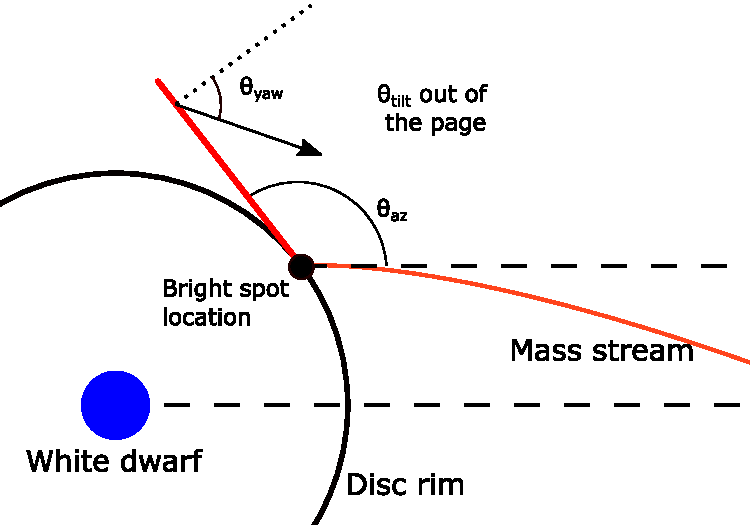
\includegraphics[width=0.7\textwidth]{figures/modelling/bright_spot_schematic.pdf}
    \caption{Showing a schematic of the bright spot model. The {\bf lower dashed line} joins the centres of the white dwarf and donor stars, and the {\bf upper dashed line} runs parallel to it, intersecting the bright spot location. The {\bf straight red line} is one half of the flux-emitting strip and has a profile exponent $Y$, and the {\bf arrow} shows the direction of light emission, at an angle $\theta_{\rm yaw}$ from the normal.}
    \label{fig:modelling:bright spot schematic}
\end{figure}

Lower values of $q$ will cause the ballistic stream to take a wider arc towards the white dwarf, moving the intersection point with the disc. The angle between the bright spot and disc edge is defined by $\theta_{\rm az}$, the angle between the strip and the line of sight of the observer.

As the bright spot is the most complex component of the model, there is an option to simplify it in software for systems with faint bright spot features that cannot be properly resolved.
This mode is called the `simple' bright spot model, and fixes $\theta_{\rm tilt}$ at $90^\circ$, $\theta_{\rm yaw}$ at $0^\circ$, and the strip exponents $X$ and $Y$ to 1 and 2, respectively. By removing these four degrees of freedom, better and faster characterisation of the eclipse is possible.

\subsubsection{Choice of priors}

The choice of prior is important in Bayesian inference, but we have very little prior knowledge on a system. The prior distributions used were generally uniform and span the numerically allowed range\footnote{e.g.\ angles are limited to be between 0 and $2\pi$, and fluxes range from 0 to the peak flux of the eclipses.}, with a few exceptions.

As it is unconstrained by data, $u_{\rm ld}$ initially uses a Gaussian prior centred on 0.3 with a width of 0.1.
The bright spot scale draws from a log-uniform prior between 0 and 0.2, which favours smaller values, and $\theta_{\rm az}$ is forbidden from values that would cause the bright spot strip to deviate from a tangent to the disc by $>80^\circ$.
In addition, some combinations of parameters are forbidden in the model. The values of $q$ and $\Delta\phi$ must be such that $i \leq 90^\circ$ for an eclipse to occur, and the disc radius is constrained by the maximum radius before precession becomes a significant effect, $R_{\rm disc} / a < 0.46$.\todo{REF}


\subsection{Post-processing the eclipse model}
\label{sect:modelling:post processing the eclipse model}

The eclipse modelling uses proxy variables, so some processing must be done to convert them to physical values. This is done in two steps. First, a white dwarf temperature and surface gravity are fit to the white dwarf fluxes. Then, the white dwarf temperature and orbital period are combined with the best-fit eclipse model parameters to convert the scaled distances to metres, and mass ratio to the masses of each star.

\subsubsection{Fitting white dwarf colours}
\label{sect:modelling:fitting white dwarf colours}
By modelling the eclipse in multiple bands, at least three observations of white dwarf flux are available.
The DA white dwarf cooling model from \citet{Bergeron1995}\footnote{Available at \href{http://www.astro.umontreal.ca/~bergeron/CoolingModels}{http://www.astro.umontreal.ca/~bergeron/CoolingModels}} is fit to these flux observations.
These cooling models yield the absolute magnitude of the white dwarf in each band, $M$, for a given effective temperature, $T_{\rm eff}$ and surface gravity, $\log (g)$. This absolute magnitude is then easily translated to an apparent magnitude, $m$, given a system parallax, $\pi$, and interstellar extinction coefficient, ${\rm E(B-V)}$,
\begin{equation}
    m = M - 5\log (\pi\mathrm{,\ arcsec}) - 5
\end{equation}

To optimise these four parameters, an affine-invariant MCMC with three levels of parallel tempering was used, c.f. \S\ref{sect:modelling:parallel tempering}. for priors, uniform $T_{\rm eff}$ and $\log (g)$ distributions were used that span the range set by the model cooling tracks. ${\rm E(B-V)}$ used a uniform distribution between 0, and the maximum IRSA measurement for the relevant sky coordinates\footnote{Available at \href{https://irsa.ipac.caltech.edu/applications/DUST/}{https://irsa.ipac.caltech.edu/applications/DUST/}}, and the parallax prior was chosen to match the Gaia measurement of the system \citep{lindegren2018, Luri2018, Gaia2016, Gaia2018}.

\subsubsection{Conversion of proxy variables to physical parameters}
\label{sect:modelling:conversion to physical parameters}
The eclipse model proxy variables are then converted to real values.
Five input variables are needed: $T_{\rm eff}$, $P_{\rm orb}$, $q$, $\Delta \phi$, and $R_{\rm wd} / x_{l1}$.


A measure of the white dwarf radius, $R_{\rm wd}$, can be found using Kepler's 3rd law and making the substitutions $r = R_{\rm wd} / a$ and $q = M_{\rm donor} / M_{\rm wd}$.
\begin{align}
    P_{\rm orb}^2 &= \frac{4 \pi^2 a^3}{G (M_{\rm wd} + M_{\rm donor})} \\[8pt]
    &= \frac{4 \pi^2 R_{\rm wd}^3}{G M_{\rm wd} (1 + q) r^3} \\[8pt]
    R_{\rm wd}^3 &= \frac{P_{\rm orb}^2 r^3 G M_{\rm wd} (1 + q) }{4 \pi^2}
    \label{eqn:modelling:geometric radius}
\end{align}
$r$ can be found from $R_{\rm wd} / x_{l1}$ by calculating $x_{l1} / a$, which itself is a function only of $q$.

Finding $R_{\rm wd}$ this way requires the white dwarf mass. Fortunately, for a given $T_{\rm eff}$ (which is known from the colour fits, \S\ref{sect:modelling:fitting white dwarf colours}), white dwarfs follow tight theoretical mass-radius relationships \citep{parsons2017}, that can be employed to find the unique $M_{\rm wd},\ R_{\rm wd}$ pair that satisfies both Equation~\ref{eqn:modelling:geometric radius} and the theoretical mass-radius relationship.
Specifically, a proposed theoretical mass-radius pair is chosen from a model relationship and a value of $R_{\rm wd, calc}$ is calculated from Equation~\ref{eqn:modelling:geometric radius}. If this matches the theoretical value, the mass is valid. Otherwise, the proposed mass is altered accordingly and a new mass-radius pair is checked again until the two agree.

Three white dwarf mass-radius relations were used. First, a solution was searched for using the \citet{wood1995} models, spanning masses of $0.4 - 1.0 M_\odot$. The \citet{wood1995} models are preferred, as they use a thicker hydrogen layer that is more appropriate for the accreting CV white dwarfs.
If no solution could be found, the \citet{panei2000} models were searched, spanning masses from $0.4 - 1.2 M_\odot$.
Both of these mass-radius relationships account for the white dwarf $T_{\rm eff}$.
If no solution has been found with these two tracks, the \citet{hamada1961} 0 Kelvin mass-radius relation is checked for solutions. This track spans the largest range in mass, from $0.14 - 1.44 M_\odot$. If no solution is found with the \citet{hamada1961} tracks, the model is considered invalid, though this did not occur for any system in this thesis.

Then, the inclination is calculated. $\Delta \phi$ is solely a function of $q$, and $i$. Therefore, we can use the eclipse model values of $\Delta\phi$ and $q$ to calculate the system inclination - this is done by proposing candidate values of $i$, and comparing the calculated $\Delta \phi_{\rm calc}(q,i)$ with the modelled $\Delta \phi$, and adjusting $i$ as needed until the two agree.

Now, three quantities are known; $i$, $M_{\rm wd}$, and $R_{\rm wd}$. As previously mentioned, $R_{\rm donor}$ is assumed to be the Roche radius, from Equation~\ref{eqn:introduction:eggleton approximation}, and $M_{\rm donor}$ is found simply by $(q \cdot M_{\rm wd})$. $a$ is calculated from the two component masses and $P_{\rm orb}$, using Kepler's laws. Finally, the orbital velocities, $K_{\rm wd,\ donor}$ respectively, of the two stars are calculated using Kepler's laws.
\begin{align}
    K_{\rm wd} &= \frac{2\pi a \mathrm{sin}i}{P_{\rm orb}} \frac{q}{1+q} \\
    K_{\rm donor} &= K_{\rm wd} \cdot \frac{M_{\rm wd}}{R_{\rm wd}}
\end{align}


\subsection{Capturing flickering with Gaussian Processes}

CVs almost always display some amount of stochastic variability, known as flickering. Rather than attempting to model this physically, it is instead treated as correlated noise and characterised with a Gaussian process (GP).
The application of GPs to capturing flickering was established by \citet{McAllister2017} based on work by \citet{roberts2012} and \citet{gibson2012}.
The utility of this addition to the eclipse modelling step is a significant improvement in the accuracy of parameter posteriors, as the GP can be used to subtract flickering from the observations while leaving the key lightcurve features that modelling aims to reproduce, demonstrated by \citet{McAllister2017}.

This section is aimed at giving a working knowledge of GPs in the context of characterising flickering, and for more in-depth discussion the reader is directed towards these works. The mathematics below omits error in flux for legibility, but closely similar derivations are possible that include error when calculating the likelihood of a data set.

\subsubsection{Gaussian Process background}
\label{sect:modelling:GP background}

GPs are a statistical method that can be adapted to produce a series of correlated points across a time (or space) axis, the distribution of which is described by a Gaussian function. The points are related to one another by a joint distribution; to illustrate what a joint distribution is, take the example to two variables $t_1, t_2$, shown graphically in Figure~\ref{fig:modelling:joint distribution}. Each is normally distributed about a central value, but higher values of $t_1$ are more likely to be produced alongside higher values of $t_2$. Thus, knowing the value of $t_1$ can inform the likely value of $t_2$, written as $P(t_1 | t_2)$.

\begin{figure}
    \centering
    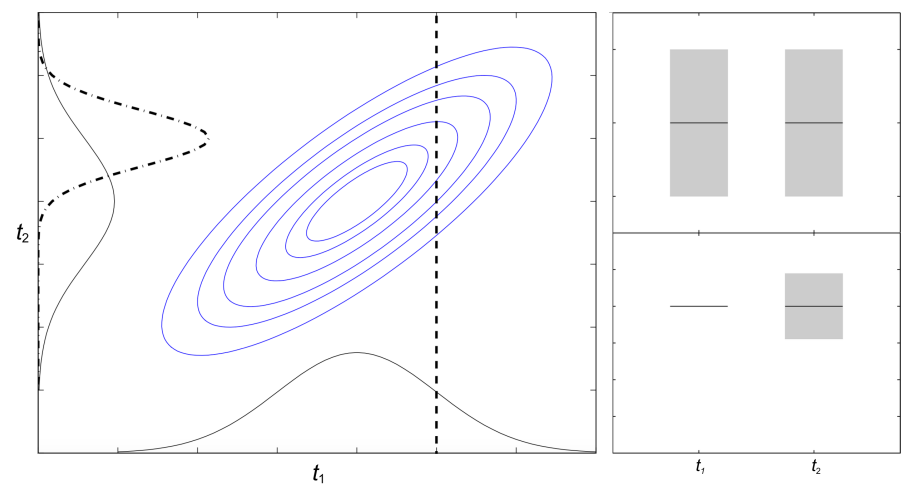
\includegraphics[width=.8\textwidth, clip, trim={0 0 8.5cm 0}]{figures/modelling/joint_distribution.png}
    \caption{Reproduced from \citet{McallisterThesis}. Two variables, $t_{1,2}$, are described by a joint Gaussian distribution. {\bf Blue ellipses} trace lines of equal probability of drawing a sample. {\bf Solid black Gaussians} along each axis show the probability distributions of each variable, and the {\bf dashed black Gaussian} along the y-axis shows the probability distribution of $t_2$, given a fixed value of $t_1$, which is shown by the {\bf vertical dashed line}.}
    \label{fig:modelling:joint distribution}
\end{figure}

By describing a time-series dataset as an arbitrarily large number of variables with a joint distribution between them, the probability of a point being described by a GP, \textit{given the rest of the data}, can be computed. Similarly, the likelihood of an entire data set being described by a GP is also calculable. This principle is the basis of time-series GPs, and allows them to be used when evaluating the goodness-of-fit of a model.

A GP distribution is defined simply by two functions, a mean function, $\mu(t)$, and a covariance function, $k(t_i, t_j)$.
\begin{equation}
    y(t) \sim \mathcal{GP}(\mu(t) \cdot k(t_i, t_j))
\end{equation}
where $t_{i, j}$ are the times of two data points, and are not necessarily adjacent. In this context, the set of $\bf y$ is a set of observed fluxes at times $\bf t$. The distribution of $\bf y$ is then represented by the joint distribution of $P({\bf y} | {\bf t})$, following a multivariate Gaussian, $\mathcal{N}$,
\begin{equation}
    P({\bf y} | {\bf t}) = \mathcal{N}(\mu({\bf t}), {\bf K})
\end{equation}
Where $\bf K$ is the covariance matrix of the multivariate Gaussian, and fully describes how the distribution of each element of $\bf t$ is affected by each other element, forming an $n \times n$ matrix for $n$ data in $\bf t$.
\begin{equation}
    {\bf K} =   \begin{pmatrix}
        k(t_1, t_1) & k(t_1, t_2) & \cdots & k(t_1, t_n) \\
        k(t_2, t_1) & k(t_2, t_2) & \cdots & k(t_2, t_n) \\
        \cdots      & \cdots      & \cdots & \cdots      \\
        k(t_n, t_1) & k(t_n, t_2) & \cdots & k(t_n, t_n) \\
            \end{pmatrix}
\end{equation}

\subsubsection{Computing a covariance matrix}
\label{sect:modelling:GP Kernel choice}

In practice, as $\bf t$ becomes a larger set and $n$ increases, computing the $n \times n$ matrix $\bf K$ becomes impractical. Instead, a kernel is defined that gives analytical functions that approximate each $k(t_i, t_j)$, and the choice of kernel defines the type of correlation between data.

When modelling flickering, a Matern-3/2 kernel is used, which produces a covariance matrix that correlates nearby values more strongly than those further away in time. The kernel has a `memory' timescale, $\lambda$, and an amplitude, $\alpha$, that can be tuned to a data set. This replaces $k(t_i, t_j)$ with $\alpha \cdot k_{M}(r^2)$, where $k_{M}(r^2)$ is defined as
\begin{equation}
    k_{M}(r^2) = \big(1+\sqrt{3r^2}\big) \cdot\exp\big(-\sqrt{3r^2}\big)\ .
\end{equation}
Here, $r^2$ is a pseudo-radius, and is a function of the distance between the two $t_{i,j}$ being considered. Generally, since the Gaussian process technique is applicable to parameter \textit{vectors}, this is written as
\begin{equation}
    r^2 = ({\bf t}_i - {\bf t}_j)^{\top} \cdot \Lambda^{-1} \cdot ({\bf t}_i - {\bf t}_j)
\end{equation}
Note that the choice of the matrix $\Lambda$ defines how other data in a set affect other data, and can be any square matrix of the same width as $\bf t$. For the GP used in this work, a simple $\Lambda$ is used which has $\lambda$ along the diagonal and 0 elsewhere, making $\lambda$ a kernel scale parameter.
In this model each $t_i$ is a single time value, making $\Lambda$ a $1\times 1$ matrix with values of $\lambda$ along the `diagonal' -- functionally, $r^2 = \lambda \cdot {(t_i - t_j)}^2$.

\subsubsection{Evaluating a model fit with a Gaussian process}
\label{sect:modelling:GP model evaluation}

Finally, the $\mathcal{L}$ of a set of ${\bf y}, {\bf t}$ can be calculated given a GP, i.e. $\mathcal{L}(\alpha, \lambda | {\bf y}, {\bf t})$, analogous to $P({\bf y} | {\bf t})$ \citep{rasmussen2006}.
This is the pertinent step to the modelling, as the likelihood function of the data is replaced with the likelihood of the GP.
When evaluating a proposed $\Theta$ in the MCMC, rather than using $\mathcal{L} \propto \mathrm{exp}(-\chi^2/2)$ the likelihood function is replaced with the likelihood of the residuals after observed fluxes have had the eclipse modelled fluxes subtracted, i.e. ${\bf y}_{\rm res} = {\bf y}_{\rm obs} - {\bf y}_{\rm model}$, given an $(\alpha, \lambda)$ pair. This is expressed more clearly algebraically, as
\begin{equation}
    \mathcal{L} = P({\bf y}_{res} | {\bf t}, \alpha, \lambda) = \frac{1}{(2\pi)^{n/2} |{\bf K}|^{1/2}} \exp \bigg(- \frac{1}{2} {\bf y}_{res}^{\top} {\bf K}^{-1} {\bf y}_{\rm res} \bigg)
\end{equation}

One final factor must be accounted for. Flickering appears to be localised to the region of space near the white dwarf, and often reduces in amplitude substantially during the white dwarf eclipse \citep{McAllister2017}.
To capture this in the GP, two kernels are used: one external to the white dwarf eclipse, and one internal to the white dwarf eclipse. Each shares a value of $\lambda$, but has its own freely variable $\alpha$, $\alpha_{\rm out}$ and $\alpha_{\rm in}$.

Overall, the GP adds three new parameters to the eclipse model: $\alpha_{\rm out, in}$ and $\lambda$, which are optimised alongside the eclipse parameters themselves. $\alpha_{\rm out, in}$ use wide, log-uniform priors to prioritise smaller amplitudes. $\lambda$ uses a narrower log-uniform prior, chosen to prevent the timescale from either exceeding the duration of the eclipse, or becoming shorter than the time resolution between data points.
The slightly more complex parameter space that must now be explored, and more computationally expensive evaluation of $\mathcal{L}$, is made up for in a significantly better characterisation of lower quality eclipses \citep{McAllister2017}.



\subsection{Hierarchical model structure}
\label{sect:modelling:optimising eclipse model parameters}

In this thesis, the lightcurve fitting model used by \citet{McAllister2019} is extended, adopting a hierarchical approach to reduce model complexity.

Changes in the disc radius and brightness profile, and bright spot parameters can mean that the same CV has a significantly different eclipse lightcurve at different times, often making it difficult to justify averaging together many eclipses, as features can become smeared out and uninformative. In the worst-case scenario, all 18 parameters would be independently variable for each eclipse, in each band. However, by sharing some parameters between eclipses and bands, this large number of free parameters is slightly reduced, and the posterior of some parameters can be informed by multiple eclipses. \citet{McAllister2017} share $q,\ R_{\rm wd} / x_{l1}$, and $\Delta\phi$ between eclipses, and we broaden that concept by organising the model into a hierarchical structure, a schematic of which is shown in Figure~\ref{fig:modelling:hierarchical_model}.

\begin{figure}
    \centering
    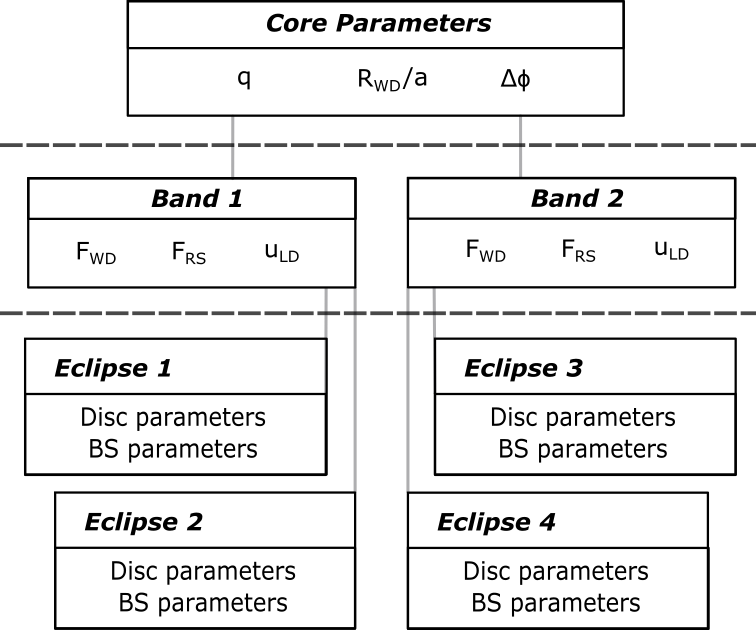
\includegraphics[width=.85\columnwidth ]{figures/results/three_cvs_with_weird_colours/GeneralFigs/hierarchical_model_structure.png}
    \caption{The hierarchical structure of the lightcurve model. Parameters are inherited downwards, to produce an eclipse at the `leaves' of the tree, e.g. Eclipse 3 inherits the parameters of Band 2, which in turn inherits the Core parameters. $\mathrm{F_{WD, RS}}$\ represent the fluxes of the white dwarf and donor star, and $\mathrm{U_{LD}}$\ is the limb darkening coefficient of the white dwarf.}
    \label{fig:modelling:hierarchical_model}
\end{figure}

The top level of the model provides the core parameters, which are unchanging between all observing bands and constant across our observations: $q,\ R_\mathrm{WD}/a$, and $\Delta\phi$. We assume the white dwarf and donor fluxes do not change on the timescale of our observations, and so these variables, along with the limb darkening coefficient of the white dwarf, are shared between all eclipses observed with the same filters. The bottom level holds parameters that can vary quickly enough to change between eclipses, i.e. parameters describing the accretion disc and bright spot. By handling parameters this way, we maximise the amount of data informing important variables. We also somewhat reduce the number of free parameters, which aids in model fitting, but the chief justification for the hierarchical approach is that it ensures consistency between eclipses - something not guaranteed when fitting eclipses individually.

Where possible, data were also binned together. Ideally, this has three beneficial effects: the number of eclipses, and therefore the number of parameters, is reduced; binning increases the signal-to-noise ratio of the data; and as the flickering component is not consistent between eclipses, should reduce the degree of flickering present in the data. However, as CV eclipses often have variable bright spot and disc contributions, it is frequently not reasonable to combine eclipses. Varying bright spot and eclipse features will become smeared out when binned, corrupting crucial elements of the eclipse.
This smearing effect is also subtly present, even in data that are consistent. As a bin width must be chosen that will not precisely align with the integration times of the photometric data, binning will always introduce a small blurring of timing data, and whilst this is a small effect, it can significantly alter the white dwarf ingress and egress features.
Therefore, binning is only done when data are sufficiently similar, and is treated with caution.



\section{Evolutionary modelling}
\label{sect:modelling:evolutionary modelling}

Once armed with a robust sample of CVs donor masses and radii, evolutionary modelling is able to refine our understanding even further. In \S\ref{sect:introduction:Summary of how AML and Mdot drive period evolution}, I motivated how the donor star inflates in response to mass loss, and how the degree of this inflation is related to the severity of the mass loss.
If the radius of an equivalent star in the absence of mass loss is known, and the observed radius of a CV donor can be reproduced by stellar structure models with the introduction of some amount of mass loss, the long-term average mass loss rate can be inferred.

The stellar evolution code used is the MESA codebase \citep{paxton2011,paxton2013,Paxton_2015,paxton2019}, a one-dimensional stellar evolution model. MESA is highly flexible, due to its use of various `modules', wherein each module supplies the code with an element of the physics of the star. These are configurable with relatively simple input files, and can be customised to extend MESA with new physics not contained in the core codebase.
Regarding CV modelling in particular, there is \textit{a priori} cause for confidence; largely default MESA configurations are capable of modelling CV donor tracks with impressive accuracy, even reproducing the period gap by a shutdown of magnetic braking triggered by the donor becoming fully convective \citep{Paxton_2015}.
\S\ref{sect:results:reproducing K11 tracks} also demonstrates this capability, and shows that with some small modifications the agreement between MESA and \citet{knigge11} can be improved further.

Note that all MESA models for this thesis were run using version 21.12.1 of the MESA codebase, and use the configuration detailed in \S\ref{sect:modelling:MESA configs}, unless specified otherwise.

To extract mass loss rates, I will go through three steps.
Firstly, I demonstrate how the radius of a singleton model of a given mass can be tuned to match the M dwarf mass-radius relationship given by \citet{BrownPrep} by introducing star spots, and produce a set of M dwarf models that reproduce observations of stars across the CV donor mass range that \textit{aren't} losing mass.
Secondly, I explore the range of masses for which the radius is a reasonable diagnostic for present-day mass loss rate.
Finally, I outline the method by which I search for mass loss rates that produce stellar models matching CV donor observations.
% Note that all code used for these steps is publicly available online.\todo{But not until Meridith says so!!!!!!}


\subsection{MESA configuration for low-mass M dwarfs}
\label{sect:modelling:MESA configs}

Broadly speaking, when computing a stellar evolution model one must simply input models of physical processes, describe some initial conditions, and allow the stellar model to evolve over time. Unfortunately, the physics of stars in not completely understood, and the processes that affect a star's evolution significantly differ depending on its conditions.
Whilst some core physics is fixed, MESA provides many options for which prescriptions to use for a particular process, or even which processes to consider at all.
MESA has default configuration vales that are reasonable for some common stellar conditions, but some tuning of the model physics is a necessary step for any rigorous modelling.
As such, some tailoring of configuration files must be done in order to produce accurate donor models.

Parameters that are not discussed below are left as the MESA default.
Notably left as default is the metallicity of the donor stars; robust measurements of donor metallicity are challenging, though some recent attempts have yielded results \citep{harrison2016,harrison2018}. However, these are prone to systematic error, and refer to a small sample size. All MESA models presented here assume a solar initial metallicity.


\subsubsection{Model initialisation}

Whilst MESA allows for beginning a MESA run with a precomputed stellar model, the models in this analysis all generate their stars from a pre-main sequence cloud of gas before each run. This ensures that each model is computed from the very beginning with the correct physics, and is set by the command \lstinline{create_pre_main_sequence_model = .true.}


\subsubsection{Nuclear processing}

Computing the equilibrium reaction rates of nuclear burning in a star is non-trivial, as the different species being consumed and produced form a complex network of interactions.
The products of one reaction are often the reagents of another, and with many options for reaction paths and hard-to-calculate reaction rates, this is prohibitive (and often inaccurate) to compute on the fly. Rather, a pre-calculated or empirical reaction network is used.

MESA has several options for the reaction network available in its core codebase. By default, the \lstinline{basic} network considers the reactions of the staple elements of most stellar cores: hydrogen-1, helium-3, carbon-12, nitrogen-14, oxygen-16, neon-20, and magnesium-24.
However, we use the more complete reaction network given by \lstinline{pp_and_cno_extras}. This is a combination of two other networks, \lstinline{pp_extras} and \lstinline{cno_extras}.
\lstinline{pp_extras} is preferred, as it more accurately represents nuclear reactions in young stars \citep{murphy2021}, and \lstinline{cno_extras} more fully considers the reaction chains the CNO cycle, specifically at high temperatures \citep{paxton2011}. To enable this, the lines \lstinline{change_net = .true., new_net_name= `pp_and_cno_extras.net'} are added to the configuration file.

In addition, the JINA Reaclib reaction rate library \citep{cyburt2010} is used: \lstinline{set_rates_preference = .true., new_rates_preference = 2}


\subsubsection{Surface boundary lookup tables}
\label{sect:modelling:MESA surface boundary tables}

When solving the four differential equations necessary to produce an internally consistent stellar model, i.e. how the radius, pressure, luminosity, and temperature vary with mass, some boundary conditions are required.
The boundary conditions for radius and luminosity are self-evident: $R(M = 0) = 0$, and $L(M = 0) = 0$. Unfortunately, such simple fixed central values are not available for the temperature and pressure, so the boundary condition at the surface of the star is used instead.
This requires defining the location of the surface of the star. This is done by setting a value of optical depth, $\tau$, to use as the base of the stellar atmosphere.

A basic approach is to set the pressure and temperature to 0 at the stellar surface, i.e. $P(M = M_\tau) = 0$, $T(M = M_\tau) = 0$, but this is a poor approximation.
A far more accurate approximation is to pre-calculate model stellar atmospheres, which then give values of $P, T$ as a function of $\tau$, $\log(g)$, and luminosity.
Different choices of atmosphere table results in different surface temperatures and pressures, which can alter the mass-radius relation for the resulting models.

For these MESA models, the \lstinline{tau_10} grid was used, which interpolates the PHOENIX \citep{hauschildt1999, hauschildt2001} and \citet{castelli2003} stellar atmospheres (which assume solar metallicity) at $\tau = 10$ for the base of the atmosphere \citep{paxton2010,paxton2011}.
Note that none of the atmosphere tables available in MESA accurately reproduce observations of M dwarfs across the range of donor masses required. In fact, of the available tables, the \lstinline{tau_10} gives some of the less accurate modelled mass-radius relations for low mass stars.
However, this atmosphere grid was chosen as it produces stars that are {\it consistently}\ smaller than required for stars with $M < 0.3 M_\odot$, a deficit that is compensated for in \S\ref{sect:modelling:tuning star spots to observations}, using the method described in \S\ref{setc:modelling:star spot model description}. In this way, rather than relying on the atmosphere table to produce the correct stellar radii, the radius can be manually adjusted to match empirical results.


\subsubsection{Mixing length theory}

Mixing length theory is concerned with the convective boundary, where rising material dissipates its heat, reverses trajectory, and begins to sink.
Models that treat a convective layer as a hard boundary between convective and non-convective material are less able to describe observations than models that allow for some degree of overshooting of rising material past the theoretical convective boundary, before dispersing its energy \citep{prandtl1925}. This is often justified physically by a rising packet of material having some momentum that must be dissipated before reversing direction \citep{bradshaw1974}.

By reducing the degree of overshooting, the efficiency with which energy is transported from the inner regions of the star is similarly reduced, increasing $R(L)$. We decrease the default MESA overshooting of $2\times$ the pressure scale height of the convective boundary, to $1.95\times$ this scale height: \lstinline{mixing_length_alpha = 1.95}. In addition, we use the \citet{henyay1965} MLT formulation, and the following overshooting formalism new to MESA v21.12.1:
\begin{itemize}
    \setlength\itemsep{0em}
    \item \lstinline{overshoot_scheme(:)    = `exponential'}
    \item \lstinline{overshoot_zone_type(:) = `any'}
    \item \lstinline{overshoot_zone_loc(:)  = `any'}
    \item \lstinline{overshoot_bdy_loc(:)   = `any'}
\end{itemize}
% https://docs.mesastar.org/en/release-r21.12.1/reference/controls.html?highlight=overshoot_f#overshooting


\subsubsection{Model convergence and grid fidelity}

Finally, two numerical options were enabled.
The first is the MESA `gold' tolerances, which enforces tight tolerances on energy conservation.
If, after computing a time step, the sum of the energies of each model cell does not closely match the known total energy of the star, the step is rejected and re-attempted, resulting in more accurate models \citep{paxton2019}.
% If a model step has poor residuals, it is rejected and re-attempted, resulting in more accurate models \citep{paxton2019}.

Second, we apply the \lstinline{okay_to_reduce_gradT_excess = .true.} flag, which enables the \lstinline{MLT++} treatment of convection of \S7.2 of \citet{paxton2013}.
When the stellar envelope is superadiabatic and its atmosphere is radiation-dominated, the convective velocities can approach the speed of sound of the stellar envelope. This forces MESA to take extremely short time steps to try and resolve convection, and makes such envelopes prohibitive to model. The \lstinline{okay_to_reduce_gradT_excess} flag allows MESA to reduce the severity of the temperature gradient, making the star less superadiabatic, and less prone to small time steps. This is important to the star spot corrections, as it allows them to be numerically stable for a larger range of spot parameters.


\subsection{Modelling star spots in MESA}
\label{sect:modelling:starspots in MESA}

A general problem in the modelling of low mass stars is an under-estimation of their radii \citep{lopez2005}, and MESA is no exception.
Recently, \citet{BrownPrep}\todo{Get this reference. Can't be long now!} characterised a sample of $\sim 15000$ M dwarfs in detached binaries with a 5th order polynomial, referred to as the Brown relation. We use this empirical mass-radius relation as the baseline `zero mass loss' benchmark radius for comparison against models.

The difference between singleton MESA models with no mass loss and the Brown relation is shown in Figure~\ref{fig:modelling:MESA inflation over Brown relation}, however the goal is not to reproduce the Brown relation exactly; CV donors are filling their Roche lobes, so are non-spherical.
To account for this effect, \citet{knigge11} introduces a $4.5\%$ radius inflation over isolated stars, and I mirror this approach. Thus, the target radius inflation in Figure~\ref{fig:modelling:MESA inflation over Brown relation} is $4.5\%$.
\begin{figure}
    \centering
    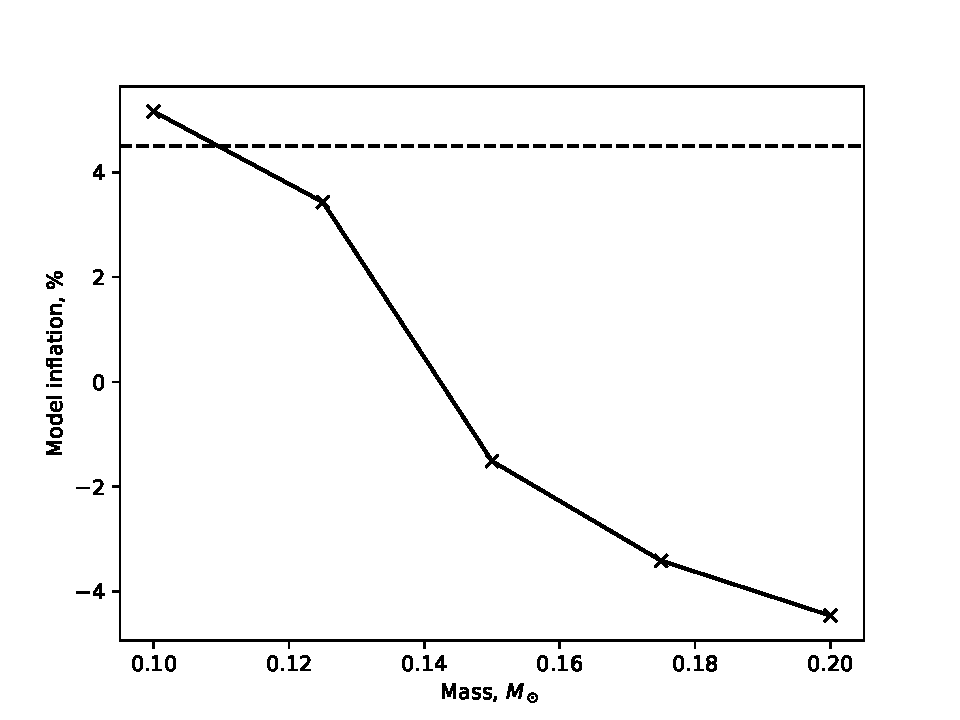
\includegraphics[width=\textwidth]{figures/modelling/MESA_inflation_over_brown.pdf}
    \caption{Showing the radius inflation of default MESA models over the Brown relation, i.e. $(R_{\rm MESA} - R_{\rm brown}) / R_{\rm brown}$. The horizontal dashed line is the target radius inflation for MESA models, of 4.5\% over the Brown relation. Crosses correspond to MESA models at an age of 2~Gyrs.}
    \label{fig:modelling:MESA inflation over Brown relation}
\end{figure}

To achieve this baseline inflation, I introduce star spots into MESA. Star spots are magnetic phenomena, where the magnetic pressure from concentrations of magnetic field lines provides partial pressure support to the photospheric material, and since spots must remain in pressure equilibrium with the spotted surface, the temperature in a spotted region is reduced by ideal gas laws. As a consequence, the cooler spotted regions emit less black body radiation, inhibiting energy flux out of the stellar interior, and inflating the star.

\subsubsection{The star spot model}
\label{setc:modelling:star spot model description}

As MESA is a one-dimensional code and star spots are a two-dimensional phenomenon, spots are modelled using the formulation given by \citet{sommers2015}, based on work by \citet{spruit1986}.
This implementation was done as a collaboration with Meridith Joyce\footnote{Accreditation} and Marc Pinsonneault\footnote{Accreditation}.

Under this spot treatment, two effects are considered: the photosphere is made inhomogeneous by the presence of spots, and convection is inhibited by the presence of a strong magnetic field.
In the \citet{sommers2015} formulation, the former effect is enforced by altering the effective temperature to a surface-weighted average of the spotted and unspotted surface, and the latter by augmenting the radiative gradient of the star.

The spots cover a fraction of the stellar surface, $f_{\rm spot}$, and a temperature contrast of $x_{\rm spot} = T_{\rm  spot} / T_{\rm amb}$, where the effective temperature of the spotted surface is $T_{\rm spot}$, and the effective temperature of the ambient, unspotted surface is $T_{\rm amb}$. The surface-weighted average of the star, $T_{\rm av}$ is then,
\begin{equation}
    \label{eqn:modelling:surface weighted average temp}
    T_{\rm av}^4 = (1-f) T_{\rm amb}^4 + f_{\rm spot} T_{\rm spot}^4
\end{equation}
And the altered luminosity, $L_{\rm av}$, becomes
\begin{align}
    L_{\rm av} =& 4\pi R^2 \sigma_{boltz} T_{\rm amb}^4 (1 - f_{\rm spot} + f_{\rm spot} \cdot x_{\rm spot}^4) \\
    L_{\rm av} =& 4\pi R^2 \sigma_{boltz} T_{\rm amb}^4 \alpha_{\rm spot} \\
    L_{\rm av} =& L_{\rm amb} \alpha_{\rm spot}
\end{align}
$\alpha_{\rm spot}$, the redistribution parameter, and is what actually alters the structure of the star. $\alpha$ is analogous to the blocking area of perfectly black spots, or spots that are completely supported by magnetic pressure.

MESA performs a lookup for the surface pressure from $T_{\rm eff}$ using precalculated boundary condition tables (\S\ref{sect:modelling:MESA surface boundary tables}). I modify the MESA code to perform this lookup with $T_{\rm av}$.

However, in MESA $T_{\rm eff}$ is not used in the stellar model interior - rather, it uses energies and pressures to calculate structure. Therefore, I alter Equation~\ref{eqn:modelling:surface weighted average temp} to use pressure instead.
Recall the ideal gas equation, for gas in the ambient, unspotted surface, this gas will have pressure and temperature $P_{\rm gas, amb}, T_{\rm gas, amb}$, density $\rho$, and mean molecular weight $\mu$. Here, $R$ denotes the gas constant.
\begin{equation}
    P_{\rm gas, amb} = \frac{\rho R}{\mu} T_{\rm gas, amb}
\end{equation}
The spotted and unspotted surfaces are under pressure
% (and therefore also density\todo{Stu disputes this - send him an email})
equilibrium, but the spotted surface pressure has a contribution from gas pressure, $P_{\rm gas, spot}$, and some contribution from magnetic pressure, $P_{\rm mag, spot}$. Therefore, we can write
\begin{align}
    P = P_{\rm gas, amb} =& P_{\rm gas, spot} + P_{\rm mag, spot} \\
    \frac{\rho R}{\mu} T_{\rm amb} =& \frac{\rho R}{\mu} T_{\rm spot} + P_{\rm mag, spot} \\[12pt]
    P_{\rm mag, spot} =& \frac{\rho R}{\mu} (T_{\rm amb} - T_{\rm spot}) \\
    % P_{\rm mag, spot} =& \frac{\rho R}{\mu} (1 - x_{\rm spot}) T_{\rm amb} \\
    P_{\rm mag, spot} =& (1-x_{\rm spot}) P_{\rm gas, amb} \\
\end{align}
And therefore,
\begin{align}
    P_{\rm gas, spot} =& P_{\rm gas, amb} - P_{\rm mag, spot}\\
    P_{\rm gas, spot} =& P_{\rm gas, amb} - (1-x_{\rm spot}) P_{\rm gas, amb} \\
    P_{\rm gas, spot} =& x_{\rm spot} P_{\rm gas, amb}
\end{align}
However, star spots do not penetrate to the core of the star. To quantify this, rather than fixing $x_{\rm spot}$ and calculating the new pressure at each depth of the star, I calculate the gas pressure differential at the surface of the star, and fix this gas pressure difference for interior layers.
As gas pressure rises with depth, a significant difference at the surface quickly becomes insignificant.
For each depth of the star, $x_{\rm spot}$ is calculated from its total pressure before any alteration is made, $P_i$, and the surface pressure, $P_{\rm surf, amb}$,
\begin{align}
    P_{\rm gas, amb} - P_{\rm mag, spot} =& x_{\rm spot} P_{\rm gas, amb} \\
    x_{\rm spot, i} =& \frac{P_i - P_{\rm surf, amb}}{P_i}
\end{align}
Rather than directly altering the pressure profile of the star, the radiative gradient, $\nabla_r$, at each depth is modified. MESA then uses $\nabla_r$ to compute a self-consistent pressure profile for the star.
\begin{align}
    \alpha_{\rm spot, i} =& 1 - f_{\rm spot} + f_{\rm spot} \cdot x_{\rm spot, i}^4 \\
    \nabla_{r,i}' =& \frac{\nabla_{r,i}}{\alpha_{\rm spot, i}}
\end{align}
Values of $f_{\rm spot}$ and $x_{\rm spot}$ can be passed to MESA as user-configured parameters to define the degree of spotting. Figure~\ref{fig:modelling:spotted model radii at 2Gyrs} shows the radii of main sequence stellar models at 2~Gyrs, and $0.15 M_\odot$ with progressively more spots. The mass-$f_{\rm spot}$ relation required to match the 4.5\% inflation over the Brown relation is searched for in \S\ref{sect:modelling:tuning star spots to observations}
\begin{figure}
    \centering
    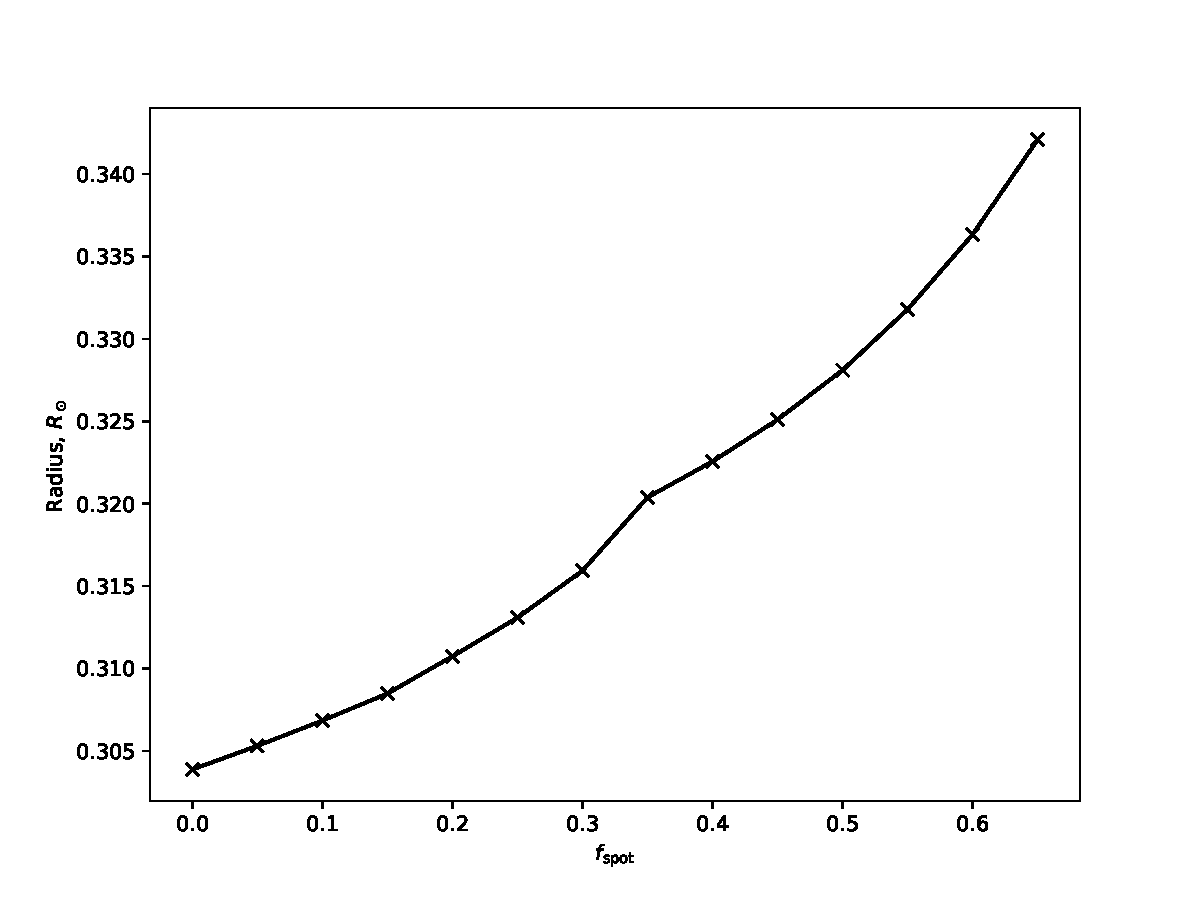
\includegraphics[width=\textwidth]{figures/modelling/spotted_model_radii_at_2gyrs.pdf}
    \caption{Showing how model radius varies as a function of spot coverage for a $0.15 M_\odot$ star. Here, spots are perfectly black ($x_{\rm spot} \equiv 0$), and the radius is extracted at 2~Gyrs. Evaluated MESA models are shown as {\bf black crosses}, and joined by a {\bf black line} to guide the eye.}
    \label{fig:modelling:spotted model radii at 2Gyrs}
\end{figure}


\subsection{Optimising mass loss rate to donor observations}
\label{sect:modelling:optimising mass loss rate to observations}

Finally, the mass loss rate required to match donor observations can be found. As the inflation of the donor increases monotonically with increasing mass loss, the binary chop algorithm is used to precisely and accurately optimise mass loss.
% To sample the error distribution of observed masses and radii, random samples were drawn from the mass and radius posterior distribution for each observation. The mean and standard deviation of the corresponding mass loss rates is reported.

An alternative approach to inferring $\dot M$ is to run a fixed grid of models, and interpolate within it.
An interpolation grid was constructed with MESA models of fixed $\dot M$ and $f_{\rm spot}$, initialised at a mass of $0.3 M_\odot$. These models were singleton stars, with the configuration described in \S\ref{sect:modelling:MESA configs}.
Values of $\dot M$ ranged from $-12<\log(\dot M)<-8$ in $\frac{1}{6}$ increments, and $f_{\rm spot}$ spanned from $0<f_{\rm spot}<-0.65$ in increments of 0.05. The initial mass value of $0.3 M_\odot$ was chosen to allow the donor to fully adjust to the $\dot M$-induced inflated radius before reaching the $0.2 M_\odot$ period gap emergence mass.

This results in a grid of model samples in a 4D cube with the axes of mass, radius, $f_{\rm spot}$, and $\dot M$.
For a given $M_{\rm donor},\ R_{\rm donor}$ pair, a value of $f_{\rm spot}$ can be interpolated from the relationship derived in \S\ref{sect:modelling:tuning star spots to observations}. Then, the grid cube can be interpolated for a value of $\dot M$.
This approach is not as accurate as the binary chop optimisation, as the radii from stellar models are not linear functions of the input parameters. However, it is orders of magnitude faster to perform, so is used to characterise the error about a central $\dot M$ value, found with the binary chop algorithm.
% The central value of the binary chop was consistent with the interpolation in all cases.

This mass loss can also be converted to an angular momentum loss rate, assuming none of the mass is retained by the white dwarf. The angular momentum of a binary is given by $J$,
\begin{equation}
    J = M_{\rm wd} M_{\rm donor} \sqrt{\frac{Ga}{M_{\rm wd} + M_{\rm donor}}}
\end{equation}
By differentiating for ${dJ}/{dM_{\rm donor}}$ with the quotient rule, we can find the AML rate by $\dot J = {dJ}/{dM_{\rm donor}} \times {dM_{\rm donor}}/{dt}$. Note that here, I assume the effect of $\dot a$ is negligible, and ignore it (a fuller, more complex treatment of the algebra confirms this -- there is a difference of $\sim 4$ orders of magnitude between the contribution to $\dot J$ from $M_{\rm donor}$ and $a$).
\begin{align}
    \frac{dJ}{dM_{\rm donor}} = M_{\rm wd} \sqrt{Ga} \bigg[ \frac{2M_{\rm wd} + M_{\rm donor}}{2 (M_{\rm wd} + M_{\rm donor})^{3/2}} \bigg] \\
    \dot J = M_{\rm wd} \dot M_{\rm donor} \sqrt{Ga} \bigg[ \frac{2M_{\rm wd} + M_{\rm donor}}{2 (M_{\rm wd} + M_{\rm donor})^{3/2}} \bigg] \label{eqn:modelling:Jdot from Mdot}
\end{align}


\subsection{Mass loss from the white dwarf properties}
\label{sect:modelling:mdot from WD temperature}

The white dwarf temperature also reveals information on the mass transfer rate, and the following summary is described more fully by \citet{townsley2009}.
In brief, as this material strikes the surface of the white dwarf the kinetic energy is converted to thermal energy, heating the white dwarf. The degree of this heating is related to the rate at which material falls to the surface -- if more material falls in, more heating is induced.
The short-term average mass loss rate, $<\dot M>$, is ultimately a function only of white dwarf mass, and temperature, given in Equation~\ref{eqn:modelling:Mdot from WD temperature}.
\begin{equation}
    \label{eqn:modelling:Mdot from WD temperature}
    T_{\rm eff} = 1.7 \times 10^4 {\rm K} \bigg( \frac{<\dot M>}{10^{-10} M_\odot {\rm yr}^{-1}} \bigg)^{1/4} \bigg( \frac{M_{\rm wd}}{0.9 M_\odot} \bigg)
\end{equation}

However, the white dwarf temperature is capable of responding to changes in $\dot M$ on $\tau_{\rm TWD} \sim 10^3 - 10^5\ {\rm yrs}$, as opposed to the $\rm \sim Gyr$ timescales of the evolutionary modelling-based method described above, so only provides a short-term snapshot of the $\dot M$ and is susceptible to corruption from outbursts.
The white dwarf temperature approach does hold a major advantage, however, in that the `zero $\dot M$' $T_{\rm eff}$ is more well-known and commonly accepted than the `zero $\dot M$' $R_{\rm donor}$ required by this newer method.

Recently, \citet{Pala2021} used spectroscopically measured $T_{\rm eff}$ and $M_{\rm wd}$ to infer the $\dot M$ of 65 CVs, the result of which is reproduced in Figure~\ref{fig:modelling:pala2022 fig13}.
The key finding from this analysis was an inverse correlation between $M_{\rm wd}$ and $\dot M$, contrary to the prediction of gravitational wave braking that lower mass systems should have lower AML rates, driving lower $\dot M$.
As the eclipse modelling of CVs produces a measure of $T_{\rm eff}$, the systems analysed for this thesis can be processed with {\it both} techniques, and have their results compared.
\begin{figure}
    \centering
    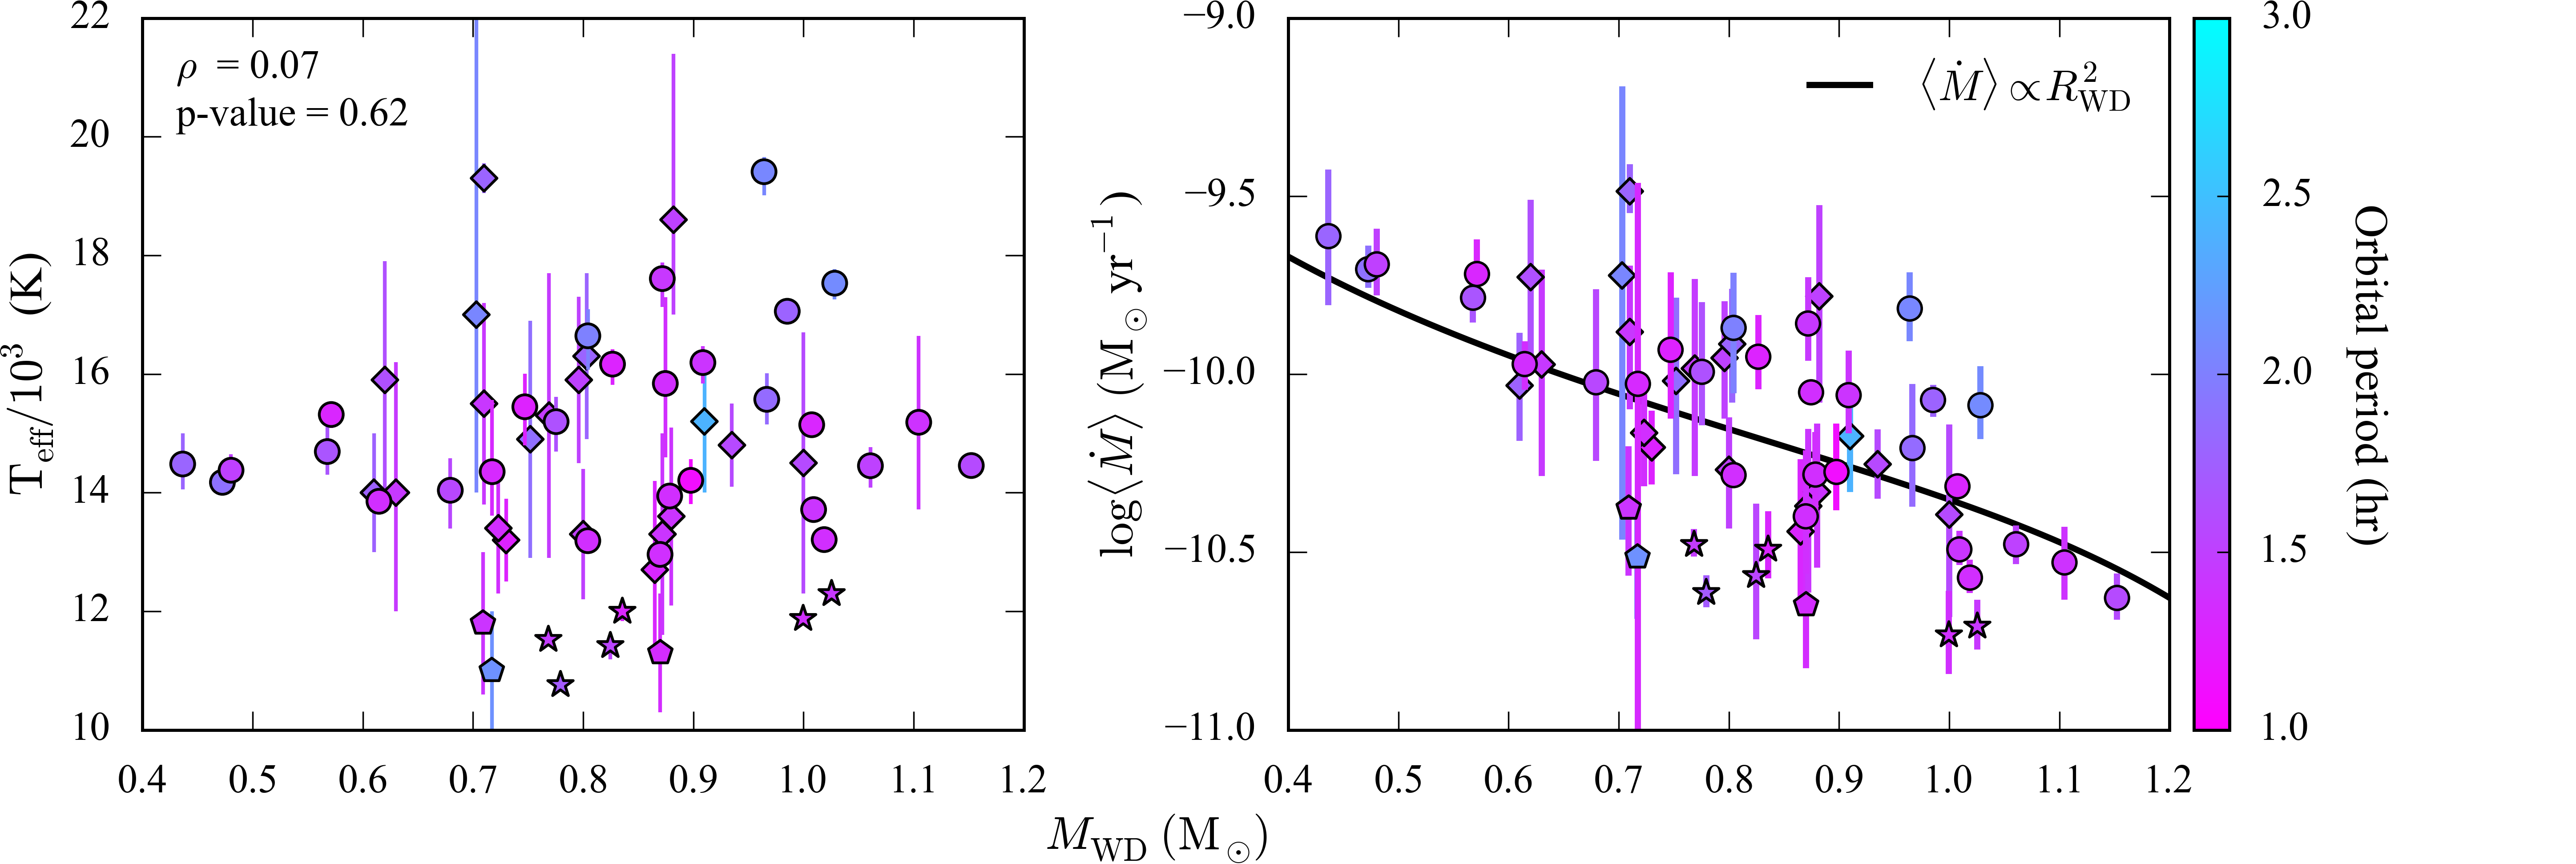
\includegraphics[width=\textwidth]{figures/modelling/pala_2022_fig13.png}
    \caption{Reproduced from \citet{Pala2021}, Figure~13. The subset of modelled systems, with $P < 3{\rm hr}$ are shown. {\bf Circles} and {\bf stars} are pre- and post-period bounce systems derived by \citet{Pala2021}, and {\bf diamonds} and {\bf pentagons} are pre- and post-period bounce systems taken from the literature. {\it Left}: The $T_{\rm eff}$ is plotted against $M_{\rm wd}$, and no correlation can be seen. {\it Right}: $\log<\dot M>$ is plotted against $M_{\rm wd}$, though now the data are correlated along the white dwarf mass-radius relationship assumed by \citet{Pala2021}, $M_{\rm wd} \propto R_{\rm wd}^1.8$. The {\bf black line} shows the rough relationship, and guides the eye.}
    \label{fig:modelling:pala2022 fig13}
\end{figure}


\chapter{Three CVs with peculiar white dwarf colours}
\label{chpt:results:three peculiar white dwarfs} % for referencing this chapter elsewhere, use \ref{chpt:label}
\lhead{\emph{Three CVs with peculiar white dwarf colours}} % This is for the header on each page - perhaps a shortened title


The work presented in this chapter was published as \cite{wild2021}, in the Monthly Notices of the Royal Astronomical Society under the title \textit{System parameters of three short period cataclysmic variable stars} by Wild, Littlefair, Ashley, Breedt, Brown, Dhillon, Dyer, Green, Kerry, Marsh, Parsons, and Sahman.
The following is my own work, unless otherwise cited.

This chapter concerns the three systems, ASASSN-16kr, ASASSN-17jf, and CRTS SSSJ0522-3505 J052210-350530 (hereafter SSSJ0522-3505), which proved challenging to model.
Phase-folded eclipse modelling gave good results in all three systems, each lightcurve being well-modelled with small residuals.
The Gaussian processes describing flickering in the systems were consistent with little to no variability, indicating that almost all the scatter in the flux residuals could be fully described by the uncertainty in flux measurement.
For a catalogue of the fits, see Appendix~\ref{appendix:lightcurves}, though an example case of ASASSN-16kr is shown in Figure~\ref{fig:three white dwarfs:ASASSN-16kr example lightcurves}.
However, when fitting white dwarf model atmospheres to the observed white dwarf fluxes, the resulting fits were not satisfactory. The bulk of this chapter discusses this poor fit, and explores its implications.

Also included is a rudimentary attempt to examine the modern understanding of CV evolution, using the excess period as a rough diagnostic of excess AML. The implications of this early method is compared to the newer, more quantitative method described in \S\ref{sect:modelling:evolutionary modelling}.

\begin{figure*}
    \centering
    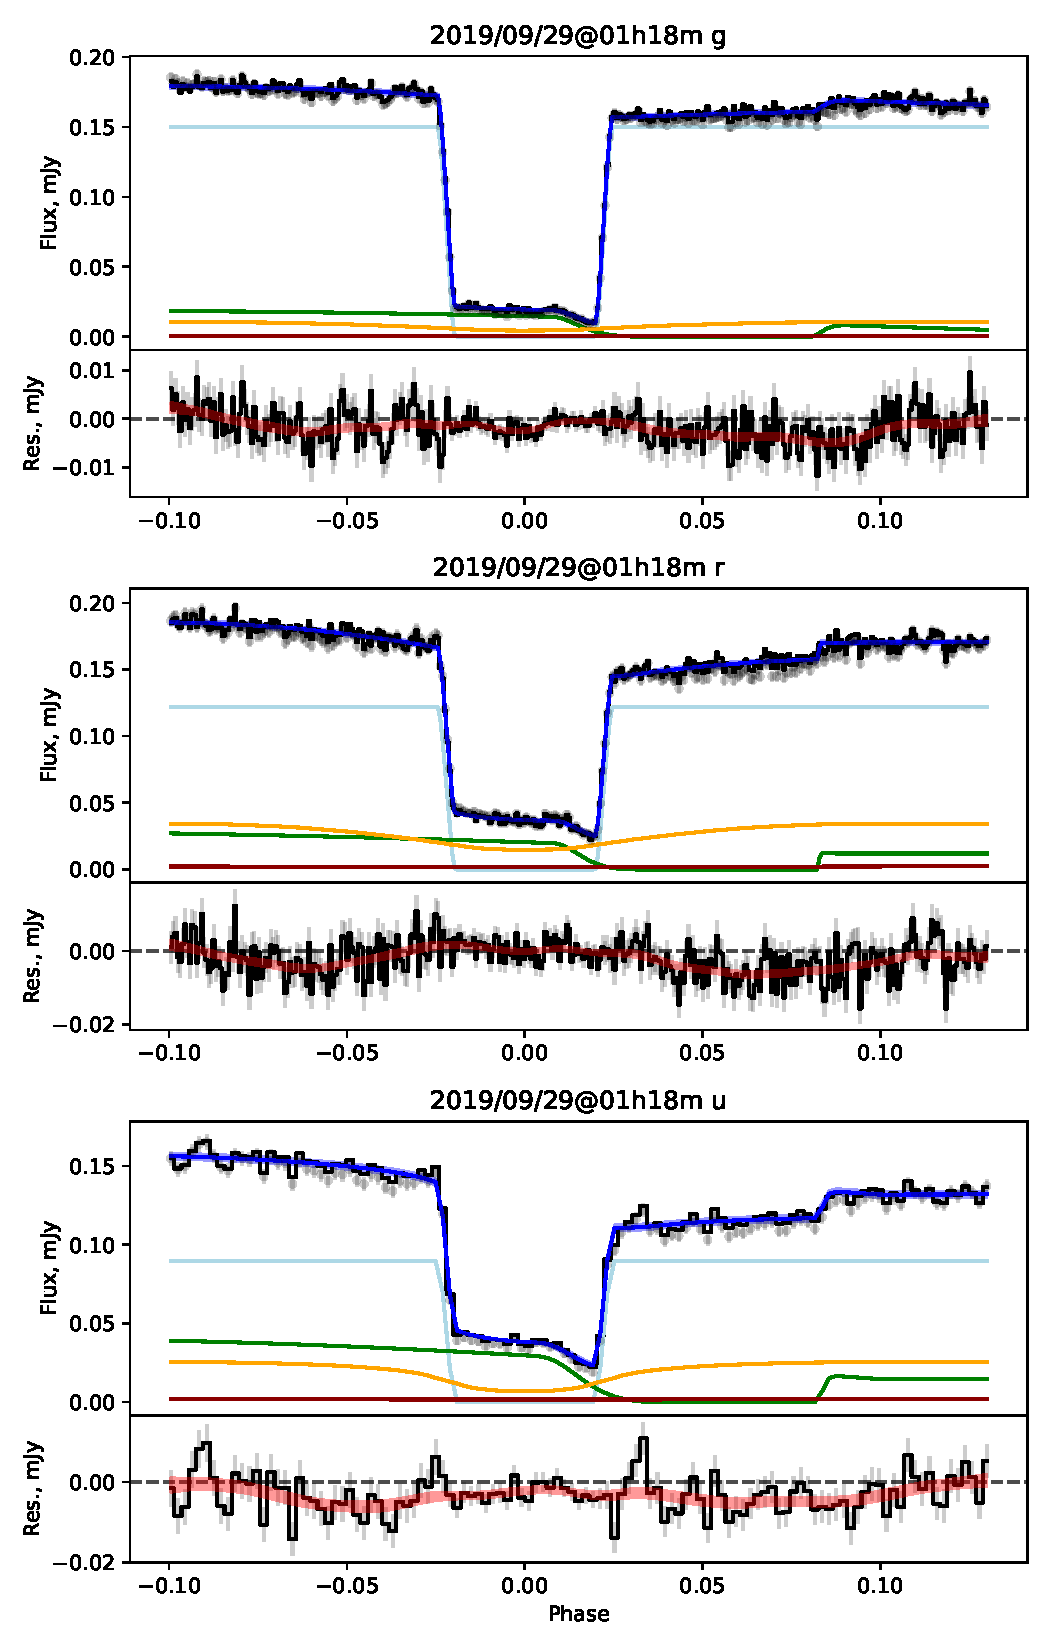
\includegraphics[width=.6\textwidth]{figures/results/three_cvs_with_weird_colours/ASASSN-16kr/ASASSN-16kr_6.pdf}
    \caption{ASASSN-16kr example lightcurve models. {\it Top}:~{\bf grey points} are the observed flux; {\bf black line} is the observed flux, with the mean Gaussian process sample subtracted; the {\bf dark blue line} is the mean lightcurve model, and the {\bf blue band} is the standard deviation on this in the MCMC chain. The components of the model are also shown: the {\bf light blue line} is the white dwarf flux, {\bf green line} is the bright spot, {\bf orange line} is the disc, and the {\bf red line} is the donor. {\it Bottom}:~The residuals between the data and model are plotted as the {\bf black line with grey error bars}. The Gaussian process 1-sigma region is shown as a {\bf red band}. A catalogue of all such fits in this work is given in Appendix~\ref{appendix:lightcurves}.}
    \label{fig:three white dwarfs:ASASSN-16kr example lightcurves}
\end{figure*}

\begin{table*}
    \centering
    \caption{The system parameters found for the three CVs with peculiar white dwarf colours. Here, the reported $\pi$ is the posterior distribution from fitting the white dwarf fluxes, c.f. \S\ref{sect:modelling:fitting white dwarf colours}.}
    \label{table:three white dwarfs:system_parameters}
    \begin{tabular}{cccc}
        \hline \\
        \textbf{System Name:}      & \textbf{ASASSN-16kr}    & \textbf{ASASSN-17jf}  & \textbf{SSSJ0522-3505} \\
        \hline \hline \\
        $M_\mathrm{WD}/M_\odot$    & $0.952\pm0.018$         & $0.669\pm0.031$        & $0.760\pm0.023$ \\
        $R_\mathrm{WD}/R_\odot$    & $0.0083\pm0.0002$       & $0.0120\pm0.0004$      & $0.0112\pm0.0003$ \\
        $M_\mathrm{donor}/M_\odot$ & $0.042\pm0.001$         & $0.060\pm0.008$        & $0.042\pm0.004$ \\
        $R_\mathrm{donor}/R_\odot$ & $0.105\pm0.002$         & $0.112\pm0.004$        & $0.105\pm0.004$ \\
        $q$                        & $0.044\pm0.002$         & $0.085\pm0.006$        & $0.055\pm0.003$ \\
        \hline
        $P$, hours                 & $1.470862368(2)$        & $1.36297(2)$           & $1.492642(2)$ \\
        $a/R_\odot$,               & $0.653\pm0.005$         & $0.567\pm0.009$        & $0.614\pm0.007$  \\
        $i$                        & $86.4\pm0.4$            & $83.7\pm0.5$           & $83.8\pm0.3$  \\
        $K_\mathrm{WD}$, km/s      & $22.7\pm1.5$            & $39.5\pm4.2$           & $26.0\pm1.8$  \\
        $K_\mathrm{donor}$, km/s   & $515\pm3$               & $462\pm5$              & $470\pm4$  \\
        \hline
        $\pi$, mas                 & $6.58\pm0.22$           & $2.09\pm0.19$          & $1.81\pm0.11$  \\
        $T_{\rm eff}$, kK          & $10-12$                 & $8-13$                 & $\sim25$  \\
        $\log(g), {\rm cgs}$  & $8.55\pm0.03$           & $8.15\pm0.05$          & $8.22\pm0.04$  \\
        \hline
    \end{tabular}
\end{table*}


\subsection{White dwarf atmosphere fits}
\label{sect:three white dwarfs:method WD atmosphere fits}

The two values of $\log (g)$ produced by modelling -- the first from fitting the white dwarf fluxes to model atmospheres, and the second from combining $T_{\rm eff}$ and $P$ with the lightcurve parameters -- did not fall within $1\sigma$ of each other in any of these three systems.
In ASASSN-17jf and SSSJ0522-3505, the white dwarf atmosphere fit converged close to the minimum surface gravity allowed by the coverage of our models, $\log(g) = 7.0$.
The second $\log (g)$, from lightcurve fitting, indicated values for each system of $8.10\pm0.04$ and $8.30\pm0.03$, respectively.
When analysing ASASSN-16kr, flux fitting gave a more reasonable $\log(g)=8.21\pm0.13$, but the second $\log (g)$ still gave a significantly higher $\log(g)=8.59\pm0.03$, a difference of $\sim3\sigma$.

This is concerning, as the two $\log (g)$\ should be consistent with one another for each system.
Comparison of the measured white dwarf colours to the \citet{Bergeron1995} model grids in Figures \ref{fig:ASASSN-17jf colours}, \ref{fig:ASASSN-16kr colours}, and \ref{fig:SSSJ0522-3505 colours}, reveals that the measured colours of the white dwarfs lie outside the colour space of the models. This is the origin of the discrepancies in $\log (g)$\ obtained with the two methods for ASASSN-17jf and SSSJ0522-3505, but ASASSN-16kr is consistent with the rightmost cooling track. However, the observed flux of a white dwarf of this radius is too high for the observed Gaia parallax, pushing the model fits to smaller, higher gravity model atmospheres.

A likely cause for this issue would be an error in photometric calibration, causing a corresponding error in white dwarf fluxes. However, this is unlikely to be the source of the problem, for the reasons explained in \S\ref{sec:observations:flux calibrating the lightcurve}.
Inspection of the figures in Appendix~\ref{appendix:lightcurves} also rules out poor lightcurve fits as the cause of this problem. The most plausible explanation for the fact that our measured white dwarf fluxes do not lie inside the model grids, is that the change in brightness during white dwarf ingress/egress is contaminated by an additional source of light, for example a boundary layer close to the white dwarf surface. The implications of this for our system parameters is discussed in \S\ref{sect:impure white dwarf discussion}.

That the white dwarf colours do not lie on the model grids also raises questions about the accuracy of the white dwarf temperatures. To try and quantify the impact on $T_{\rm eff}$, two additional optimisations of model parameters to the white dwarf fluxes were performed.
In one approach, a Gaussian prior on $\log (g)$\ using the estimate from the lightcurve modelling was used, and all available flux measurements were fit simultaneously.
In a second approach we fit the white dwarf flux in each band independently using the same prior on $\log (g)$\ and the Gaia prior on $\pi$. Since these independent fits use no colour information, E(B-V) is only constrained by the prior, but is retained as a nuisance parameter and $T_{\rm eff}$ is marginalised over E(B-V). Figure~\ref{fig:three white dwarfs:gamma fits} shows the $T_{\rm eff}$ posteriors from the individual fits for the three systems.

\begin{figure}
    \centering
    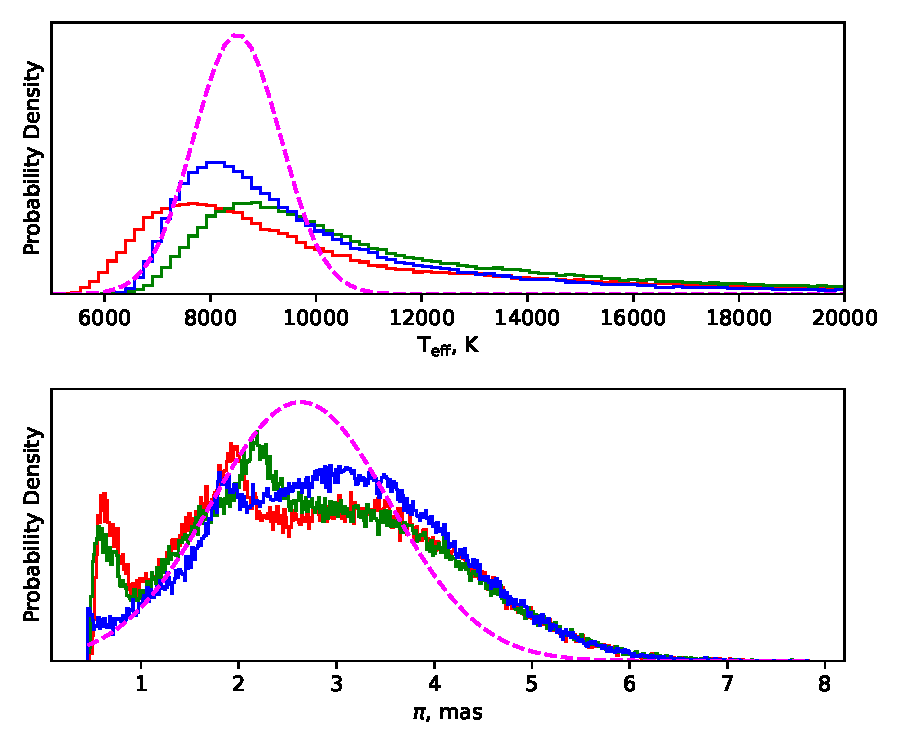
\includegraphics[width=\columnwidth, trim={0cm 6.5cm 0cm 0cm}, clip]{figures/results/three_cvs_with_weird_colours/ASASSN-17jf/PhysicalParams/all_gamma_asassn17jf.pdf}
    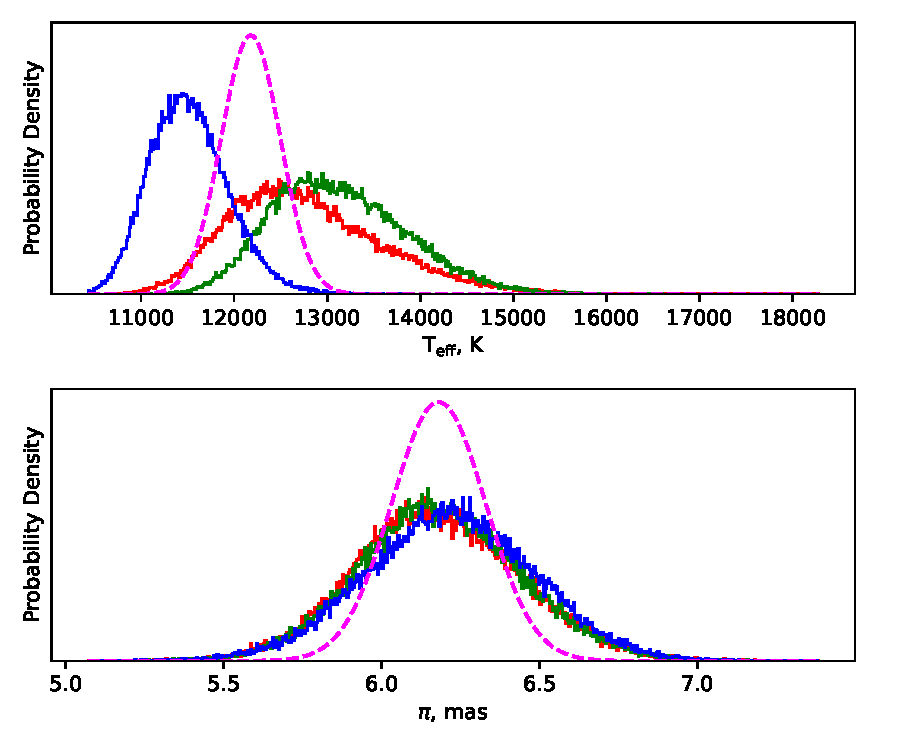
\includegraphics[width=\columnwidth, trim={0cm 6.5cm 0cm 0cm}, clip]{figures/results/three_cvs_with_weird_colours/ASASSN-16kr/PhysicalParams/all_gamma_asassn16kr.pdf}
    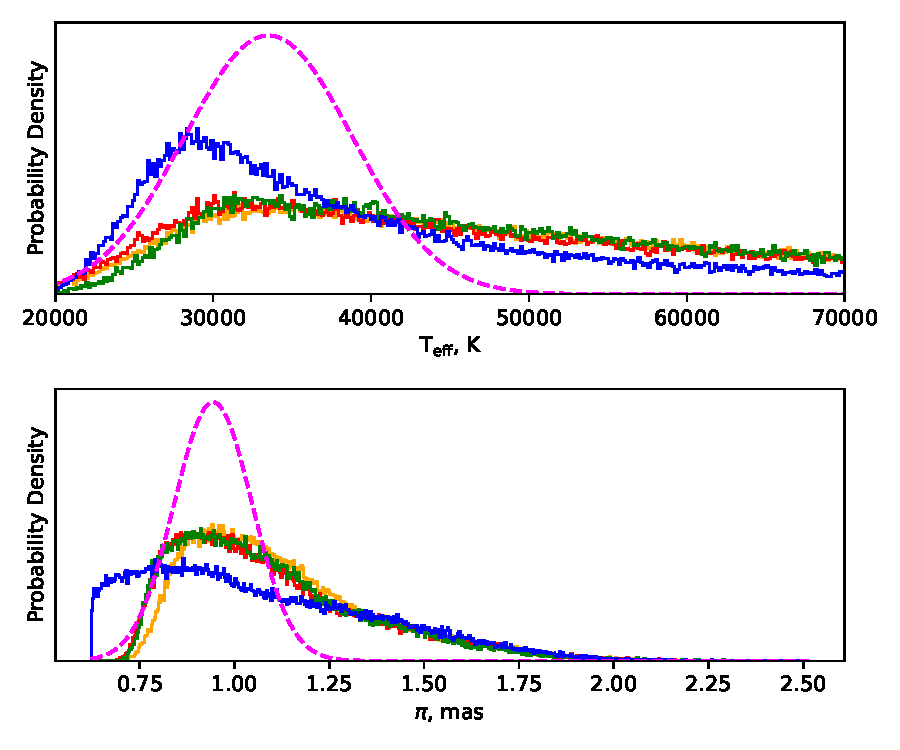
\includegraphics[width=\columnwidth, trim={0cm 6.5cm 0cm 0cm}, clip]{figures/results/three_cvs_with_weird_colours/SSS111126/PhysicalParams/all_gamma_SSS111126.pdf}
    \caption{The result of fitting white dwarf model atmospheres to each photometric band independently. {\bf Blue solid line}: $u'$ band, {\bf Green solid line}: $g'$ band, {\bf Red solid line}: $r'$ band. The joint distribution between all bands is characterised in each case by the best fit Gaussian ({\bf magenta dashed lines}). \textit{Top}: ASASSN-17jf, joint $T_{\rm eff}=8330\pm780\rm\ K$; \textit{Middle}: ASASSN-16kr, joint $T_{\rm eff}=12150\pm300\rm\ K$; \textit{Bottom}: SSSJ0522-3505, joint $T_{\rm eff}=33300\pm5200 \rm\ K$. }
    \label{fig:three white dwarfs:gamma fits}
\end{figure}

Figure \ref{fig:three white dwarfs:gamma fits} shows little sign of a consistent discrepancy over the three observed CVs. The $u'$ band in ASASSN-16kr and SSSJ0522-3505 suggests a cooler temperature than the other bands, but lies in between the $r'$ and $g'$ in ASASSN-17jf.


\subsubsection{White dwarf temperature fits}
\label{sect:white dwarf temperature report}

Each approach gives a different distribution for $T_{\rm eff}$.
To avoid confusion, results of each individual fit are not reported, instead the overall temperature ranges for each system are given.

ASASSN-16kr $T_{\rm eff}$ estimates ranged from 10200K to 12150K, and ASASSN-17jf estimates from 8330K to  12710K.
The SSSJ0522-3505 fits that used all four observed fluxes both converged on $\sim22700$K, but the single-flux fits all resulted in wide posterior distributions covering $25000 - 90000$K, with very weak peaks in the $\sim30000 - 50000$K range, seen in Figure~\ref{fig:three white dwarfs:gamma fits}.

In all three systems, the figures reported in Table~\ref{table:three white dwarfs:system_parameters} are the $T_{\rm eff}$ produced by the constrained $\log (g)$ fit with all fluxes simultaneously.
The $\log (g)$ reported are the values found from the lightcurve parameters.


\subsection{System Parameters}
\label{sect:system parameters}

The effect of the uncertain white dwarf temperatures on the system parameters, most importantly $M_{\rm wd}$, is mostly negligible. For example, increasing $T_{\rm eff}$ for ASASSN-17jf from 8000K to 12000K only changes $M_{\rm WD}$ by $0.001M_\odot$, compared to our statistical uncertainty of $0.031 M_\odot$. Even a large uncertainty in $T_{\rm eff}$ only has a minor impact on the system parameters; for example a change in the WD temp for SSSJ0522-3505 from $10000$K to $20000$K only changes $M_{\rm WD}$ by $0.02 M_\odot$, comparable with the measurement uncertainty. The system parameters are reported in Table~\ref{table:three white dwarfs:system_parameters}.

ASASSN-16kr has a recorded superhump period, and now also a $q$ measurement. It can therefore be used to calibrate the superhump period excess, $\epsilon$ vs. $q$ relationship, as done in \citet{McAllister2019}, though with a more extreme mass ratio system than was previously available. The system was not confidently classed as exhibiting stage B or C stage superhumps, so the results for both stages are given. Assuming the CV was in stage B, $q_B = 0.059\pm0.007$; assuming stage C and using the relevant relation from \citet{McAllister2019}, $q_C = 0.068\pm0.012$. In both cases, the estimated $q_\mathrm{B,C}$ is $\sim 2 \sigma$ higher than the observed value of $q = 0.044\pm0.002$. While a $2 \sigma$ difference is not a highly significant discrepancy, this may be preliminary evidence that the $\epsilon - q$ relation may over estimate $q$ for CVs at short periods, which has been suspected for some time \citep{pearson2007, knigge11}.

\begin{figure}
    \centering
    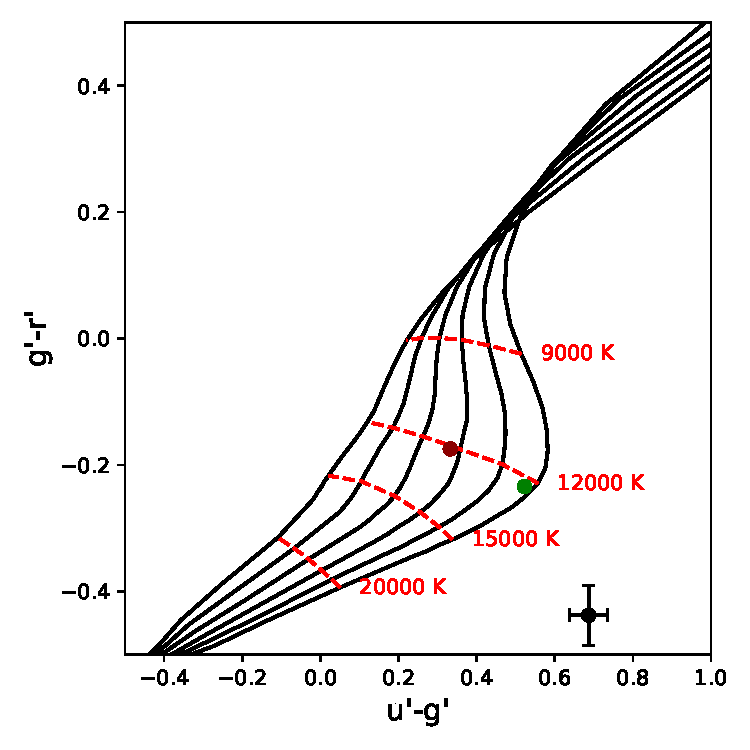
\includegraphics[width=\columnwidth, trim={0 0mm 0 0},clip]{figures/results/three_cvs_with_weird_colours/ASASSN-17jf/PhysicalParams/ASASSN-17jf_colourPlot_alpha_beta.pdf}
    \caption{The white dwarf model atmosphere fits for ASASSN-17jf. {\bf Green circle}: Best fit with uniform prior on $\log (g)$. {\bf Red circle}: Best fit with the prior $\log(g)=8.10\pm0.04$. The observations are shown as the {\bf black point and error bars}. {\bf Solid black lines} are white dwarf model cooling tracks, increasing in $\log (g)$\ to the left. {\bf Red dashed lines} are isothermal tracks for different $\log (g)$.}
    \label{fig:ASASSN-17jf colours}
\end{figure}
\begin{figure}
    \centering
    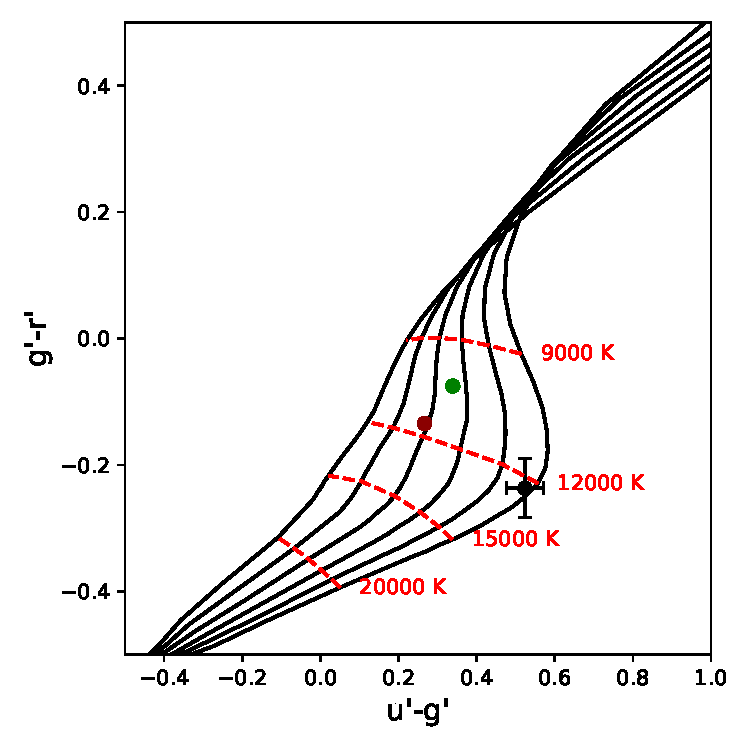
\includegraphics[width=\columnwidth, trim={0 0mm 0 0},clip]{figures/results/three_cvs_with_weird_colours/ASASSN-16kr/PhysicalParams/ASASSN-16kr_colourPlot_alpha_beta.pdf}
    \caption{The white dwarf model atmosphere fits for ASASSN-16kr. The {\bf red circle} is the best fit with a prior of $\log(g)=8.52\pm0.02$. Symbols are the same as Figure~\ref{fig:ASASSN-17jf colours}.}
    \label{fig:ASASSN-16kr colours}
\end{figure}
\begin{figure}
    \centering
    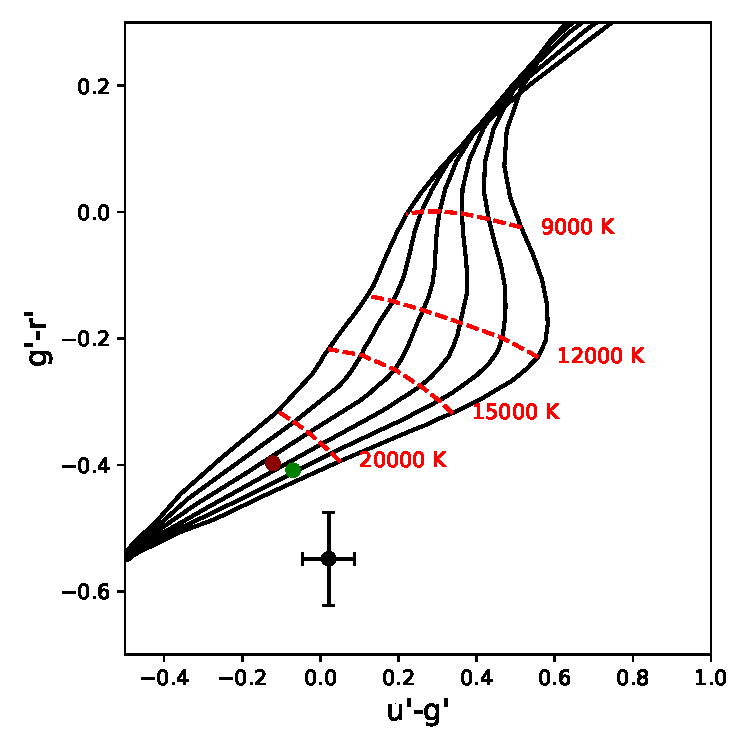
\includegraphics[width=\columnwidth, trim={0 0 0 0}, clip]{figures/results/three_cvs_with_weird_colours/SSS111126/PhysicalParams/SSS111126_colourPlot_alpha_beta.pdf}
    \caption{The white dwarf model atmosphere fits for SSSJ0522-3505. The {\bf red circle} is the best fit with a prior of $\log(g)=8.28\pm0.04$. Symbols are the same as Figure~\ref{fig:ASASSN-17jf colours}.}
    \label{fig:SSSJ0522-3505 colours}
\end{figure}



\chapter{Eclipse modelling results of 12 CVs}
\label{chpt:results:characterisation of 12 new CVs} % for referencing this chapter elsewhere, use \ref{chpt:label}
\lhead{\emph{Eclipse modelling of 12 CVs}} % This is for the header on each page - perhaps a shortened title

% As previously mentioned, a primary focus of this thesis is to grow the population of eclipse modelled CVs.
A modest backlog of observed data was reduced, calibrated, and modelled, and the results are presented here. All CVs were fit using the new hierarchical model structure described in \S\ref{sect:modelling:optimising eclipse model parameters}, with eclipses binned together where possible, to reduce the complexity of the parameter space. Which specific data were binned together for each system, if any, is given in the tables in \S\ref{sect:observing:observation catalogue}.


\section{Systems chosen for modelling}

The systems modelled here were largely chosen based on their short periods, in an effort to uncover more period-bouncer CVs, as this population is under-sampled in previous eclipse-modelled CVs.
The systems chosen for modelling range in period from $1.4 - 2.2$ hours, and were drawn from a few sources.
The All-Sky Automated Survey for Supernovae (ASASSN) \citep{shappee2014} is sensitive to transients, and is a valuable tool to identify CVs by their outbursts for follow-up once they re-enter quiescence. Such systems are recognised by their ASASSN moniker.
% The vsnet alert system also provided several systems, which are marked below with (v).
The modelled systems in this thesis were:
\begin{itemize}
    \setlength\itemsep{0em}
    \item ASASSN-14hq
    \item ASASSN-14kb (a.k.a OGLE-LMC529.30.114)
    \item ASASSN-15pb
    \item ASASSN-17fo
    \item AY For (a.k.a H$\alpha$0242-2802) \citep{woudt2004}
    \item CSS090622 J215636+193242 (hereafter CSS090622) \citep{kato2012,thorstensen2016}
    \item CSS090102 J132536+210037 (hereafter CSS090102) \citep{kato2012}
    \item CSS090419 J162620-125557 (hereafter CSS090419) \citep{kato2012}
    \item MASTER OT J001400.25-561735.0 (hereafter MAS0014) (Woudt, private communication)
    \item OGLE BLG-ECL-000082 (a.k.a BLG510.16.126296, hereafter OGLE82)
    \item SDSS J074859.6+312512.7 (hereafter SDSS J0748) \citep{kato2016}
    \item SDSS J152419.33+220920.0 (hereafter SDSS J1524) \citep{southworth2010,michel2013}
\end{itemize}

ASASSN-14hq and ASASSN-15pb were observed by \citet{paterson2019}, though the observations used in this thesis pre-date this publication. These two systems were noted to be in outburst in late 2014 in the case of ASASSN-14hq, and 2015 in the case of ASASSN-15pb.

AY For had the white dwarf and donor stars' masses estimated spectroscopically in \citet{mason2005} to be $M_{\rm wd} \sim 0.64 M_\odot$ and $M_{\rm donor} \sim 0.17 M_\odot$, with no error reported. This measurement, however, is dubious. It is based on inferring a donor mass and radius from the period using the model $M_{\rm donor} - P$ relation presented in \citet{howell2002}, which is then used to calculate a white dwarf mass. AY For is also claimed by \citet{mason2005} to be a pre-period minimum system.


\section{Results}
\label{sect:results:12 new CVs:results}

All eclipses presented are well-described by their fits, with small residuals. The lightcurves are contained in Appendix~\ref{appendix:lightcurves}, along with the white dwarf flux distributions compared to the cooling tracks, in Appendix~\ref{appendix:white dwarf fluxes}. The example system of ASASSN-14kb has the lightcurve and flux distribution is shown in Figure~\ref{fig:results:12 new CVs:ASASSN-14kb all lightcurves}, and Figure~\ref{fig:results:12 new CVs:ASASSN-14kb flux plot}, respectively.
In a few cases, the GP appears as a flat line along a residual of 0, despite some obvious scatter, for example in ASASSN-14hq, seen in Figure~\ref{fig:ASASSN-14hq all lightcurves cont}. This is expected, as in these cases the residuals are fully described by the error in flux and the GP likelihood becomes dominated by the priors, sampling small values of GP amplitude.

\begin{figure}
    \centering
    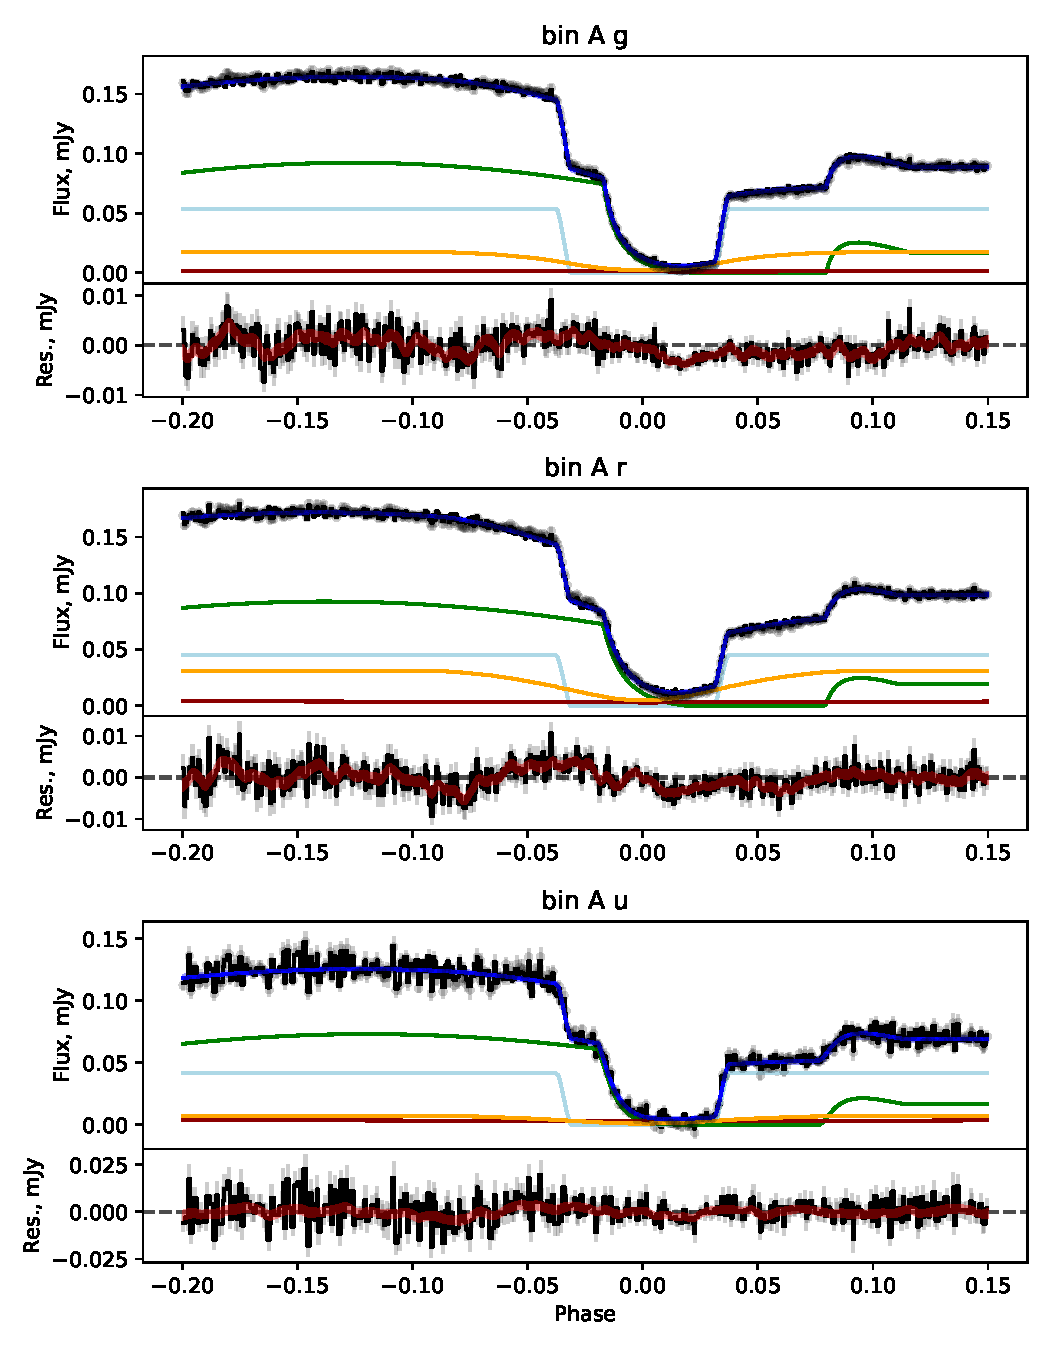
\includegraphics[width=\textwidth]{figures/results/ASASSN-14kb/ASASSN-14kb_ex_1.pdf}
    \caption{Example lightcurve models, of ASASSN-14kb. {\it Top}:~{\bf grey points} are the observed flux, and note that the photometric system is the SDSS as per \S\ref{sect:observations:flux calibrating the lightcurve}; {\bf black line} is the observed flux, with the mean Gaussian process sample subtracted; the {\bf dark blue line} is the mean lightcurve model, and the {\bf blue band} is the standard deviation on this in the MCMC chain. The components of the model are also shown: the {\bf light blue line} is the white dwarf flux, {\bf green line} is the bright spot, {\bf orange line} is the disc, and the {\bf red line} is the donor. {\it Bottom}:~The residuals between the data and model are plotted as the {\bf black line}, with grey error bars. The Gaussian process 1-sigma region is shown as a {\bf red band}.}
    \label{fig:results:12 new CVs:ASASSN-14kb all lightcurves}
\end{figure}
\begin{figure}
    \centering
    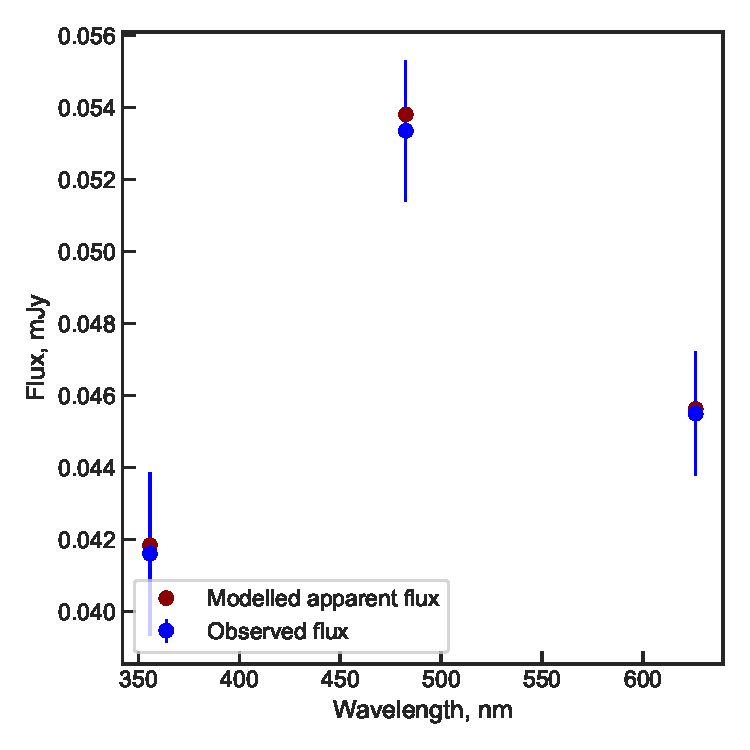
\includegraphics[width=\textwidth]{figures/results/ASASSN-14kb/fluxplot.pdf}
    \caption{The example case of the ASASSN-14kb observed white dwarf fluxes, compared to the best-fit model atmosphere.}
    \label{fig:results:12 new CVs:ASASSN-14kb flux plot}
\end{figure}

The white dwarf fluxes of AY For were not well-described by the white dwarf cooling tracks, similarly to the systems in \S\ref{sect:three white dwarfs:method WD atmosphere fits}. There is high confidence that this is a real effect rather than a poor calibration, as the field about AY For was observed by the PANSTARRS survey, and the comparison star SDSS magnitudes are reported. The flux calibration performed as standard with ULTRACAM is within 2\% of the PANSTARRS values.
In addition, the white dwarf fluxes of CSS090419 and CSS090622 appear to significantly brighten in the $i'$ band, seen in Figure~\ref{fig:CSS090419 flux plot} and Figure~\ref{fig:CSS090622 flux plot}, which cannot be described by the white dwarf models used here. However, the disagreement in each case is well within $2 \sigma$, and not seen in the other $i$ band observation, ASASSN-15pb, suggesting this is not a systematic issue. For both systems, the characterisation can still be considered robust.

Table~\ref{table:12 new cvs:system_parameters} details the physical parameters of these 12 new systems.

\newpage

\begin{landscape}

    \begin{table*}
        \centering
        \caption{The system parameters found for the CVs analysed here. The reported parallax, $\pi$, is the posterior distribution from fitting the white dwarf fluxes, c.f.~\S\ref{sect:modelling:fitting white dwarf colours}.}
        \label{table:12 new cvs:system_parameters}
        \begin{tabular}{cccccc}
            \hline \\
            \textbf{System Name:}      & \textbf{ASASSN-14hq}    & \textbf{ASASSN-14kb}     & \textbf{ASASSN-15pb}      & \textbf{ASASSN-17fo}      & \textbf{AY For}       \\
            \hline \hline \\
            $M_\mathrm{WD}/M_\odot$    & $0.67\pm0.01$           & $0.74\pm0.02$            & $0.72\pm0.03$             & $0.85\pm0.01$             & $0.78\pm0.02$         \\
            $R_\mathrm{WD}/R_\odot$    & $0.0119\pm0.0001$       & $0.0113\pm0.0002$        & $0.0115\pm0.0005$         & $0.0099\pm0.0001$         & $0.0106\pm0.0003$ \\
            $M_\mathrm{donor}/M_\odot$ & $0.097\pm0.002$         & $0.134\pm0.003$          & $0.148\pm0.008$           & $0.109\pm0.002$           & $0.106\pm0.006$ \\
            $R_\mathrm{donor}/R_\odot$ & $0.157\pm0.001$         & $0.164\pm0.001$          & $0.210\pm0.004$           & $0.1436\pm0.0007$         & $0.162\pm0.003$ \\
            $q$                        & $0.145\pm0.002$         & $0.182\pm0.002$          & $0.206\pm0.004$           & $0.1267\pm0.0005$         & $0.136\pm0.004$ \\
            \hline
            $P$, hours                 & $1.78384800(7)$         & $1.63453(1)$             & $2.23896(3)$              & $1.477147(2)$             & $1.790756(1)$ \\
            $a/R_\odot$,               & $0.681\pm0.004$         & $0.670\pm0.005$          & $0.824\pm0.014$           & $0.646\pm0.003$           & $0.717\pm0.007$ \\
            $i$                        & $80.35\pm0.06$          & $84.4\pm0.1$             & $79.4\pm0.1$              & $84.23\pm0.03$            & $84.0\pm0.2$ \\
            $K_\mathrm{WD}$, km/s      & $58.0\pm0.9$            & $76.2\pm1$               & $75\pm2$                  & $60.2\pm0.4$              & $57.8\pm2.0$ \\
            $K_\mathrm{donor}$, km/s   & $399\pm2$               & $419\pm3$                & $364\pm6$                 & $468\pm2$                 & $425\pm4$ \\
            \hline
            $\pi$, mas                 & $3.40\pm0.07$           & $2.78\pm0.11$            & $1.0\pm0.2$               & $1.79\pm0.36$             & $2.12\pm0.16$ \\
            $T_{\rm eff}$, K           & $14819\pm800$           & $17700\pm1000$           & $19200\pm1600$            & $14800\pm600$             & $18100\pm500$ \\
            $\log(g), {\rm cgs}$       & $8.11\pm0.02$           & $8.21\pm0.03$            & $8.17\pm0.06$             & $8.37\pm0.02$             & $8.28\pm0.04$ \\
            \hline
            \hline
        \end{tabular}
    \end{table*}

    \begin{table*}
        \centering
        \caption{Table~\ref{table:12 new cvs:system_parameters}, continued.}
        \label{table:12 new cvs:system_parameters cont 1}
        \begin{tabular}{cccccc}
            \hline \\
            \textbf{System Name:}      & \textbf{CSS090102}     & \textbf{CSS090419}    & \textbf{CSS090622}    & \textbf{OGLE82}   & \textbf{SDSS J0748} \\
            \hline \hline \\
            $M_\mathrm{WD}/M_\odot$    & $0.62\pm0.03$          & $0.59\pm0.08$         & $0.67\pm0.06$         & $0.83\pm0.01$     & $0.68\pm0.02$ \\
            $R_\mathrm{WD}/R_\odot$    & $0.0126\pm0.0004$      & $0.0122\pm0.0009$     & $0.0112\pm0.0007$     & $0.0099\pm0.0002$ & $0.0121\pm0.0004$ \\
            $M_\mathrm{donor}/M_\odot$ & $0.060\pm0.003$        & $0.087\pm0.011$       & $0.104\pm0.009$       & $0.131\pm0.004$   & $0.066\pm0.004$ \\
            $R_\mathrm{donor}/R_\odot$ & $0.119\pm0.002$        & $0.152\pm0.007$       & $0.155\pm0.005$       & $0.170\pm0.002$   & $0.117\pm0.002$ \\
            $q$                        & $0.094\pm0.002$        & $0.146\pm0.003$       & $0.159\pm0.008$       & $0.157\pm0.002$   & $0.095\pm0.004$ \\
            \hline
            $P$, hours                 & $1.49723786(5)$        & $1.81062621(6)$       & $1.702302(6)$         & $1.7263398(6)$    & $1.39947(1)$ \\
            $a/R_\odot$,               & $0.582\pm0.008$        & $0.660\pm0.030$       & $0.661\pm0.020$       & $0.720\pm0.006$   & $0.575\pm0.007$ \\
            $i$                        & $88.7\pm0.6$           & $80.9\pm0.1$          & $88.2\pm0.6$          & $83.9\pm0.1$      & $81.7\pm0.2$ \\
            $K_\mathrm{WD}$, km/s      & $40.9\pm1.2$           & $56.0\pm2.7$          & $63.7\pm2.5$          & $68.5\pm1.0$      & $42.2\pm1.8$ \\
            $K_\mathrm{donor}$, km/s   & $431\pm6$              & $381\pm16$            & $408\pm12$            & $435\pm3$         & $450\pm5$ \\
            \hline
            $\pi$, mas                 & $1.41\pm0.30$          & $1.42\pm0.69$         & $2.02\pm0.27$         & $3.82\pm0.12$     & $1.83\pm0.14$ \\
            $T_{\rm eff}$, K           & $14800\pm1200$         & $18200\pm9000$        & $9800\pm1500$         & $18000\pm4000$    & $22500\pm3000$ \\
            $\log(g), {\rm cgs}$       & $8.00\pm0.33$          & $8.04\pm0.12$         & $8.16\pm0.08$         & $8.37\pm0.03$     & $8.11\pm0.03$ \\
            \hline
            \hline
        \end{tabular}
    \end{table*}

    \begin{table*}
        \centering
        \caption{Table~\ref{table:12 new cvs:system_parameters}, continued.}
        \label{table:12 new cvs:system_parameters cont 2}
        \begin{tabular}{ccc}
            \hline \\
            \textbf{System Name:}      & \textbf{MASOT0014}     & \textbf{SDSS J1524} \\
            \hline \hline \\
            $M_\mathrm{WD}/M_\odot$    & $0.86\pm0.03$          & $0.80\pm0.04$ \\
            $R_\mathrm{WD}/R_\odot$    & $0.0097\pm0.0003$      & $0.0103\pm0.0005$ \\
            $M_\mathrm{donor}/M_\odot$ & $0.122\pm0.007$        & $0.074\pm0.008$ \\
            $R_\mathrm{donor}/R_\odot$ & $0.165\pm0.003$        & $0.132\pm0.005$ \\
            $q$                        & $0.142\pm0.004$        & $0.093\pm0.007$ \\
            \hline
            $P$, hours                 & $1.7167077(5)$         & $1.56764953(2)$ \\
            $a/R_\odot$,               & $0.722\pm0.008$        & $0.652\pm0.01197$ \\
            $i$                        & $84.8\pm0.3$           & $86.7\pm1.1$ \\
            $K_\mathrm{WD}$, km/s      & $63.2\pm2.0$           & $42.9\pm3.4$ \\
            $K_\mathrm{donor}$, km/s   & $445\pm5$              & $461\pm7$ \\
            \hline
            $\pi$, mas                 & $2.42\pm0.11$          & $1.92\pm0.19$ \\
            $T_{\rm eff}$, K           & $17300\pm1000$         & $12500\pm1100$ \\
            $\log(g), {\rm cgs}$       & $8.37\pm0.04$          & $8.32\pm0.06$ \\
            \hline
            \hline
        \end{tabular}
    \end{table*}
\end{landscape}


\chapter{Inferring mass loss rate from donor properties}
% \label{chpt:results:evolutionary modelling} % for referencing this chapter elsewhere, use \ref{chpt:label}
% \lhead{\emph{Inferring mass loss rate from donor properties}} % This is for the header on each page - perhaps a shortened title

\label{chpt:Mass loss and Angular momentum loss in short period CVs} % for referencing this chapter elsewhere, use \ref{chpt:label}
\lhead{\emph{Mass loss and Angular momentum loss in short period CVs}} % This is for the header on each page - perhaps a shortened title

The structure of this chapter is as follows: first, I demonstrate that MESA is capable of reproducing the canonical CV donor tracks of \citet{knigge11}, and use MESA to evaluate the range of donor masses for which the method detailed in \S\ref{sect:modelling:evolutionary modelling} can be reasonably applied.
Then, I derive an empirical relationship for appropriate spot parameters as a function of donor mass, and use this to infer $\dot M_{\rm donor}$ and $\dot J$ for the well-characterised eclipse modelled CV sample.

The analysis of this section includes eclipse modelled data from several sources: the 15 systems contained in this thesis, the 15 CVs characterised by \citet{McAllister2019}, and the 14 CVs modelled by \citet{Savoury2011}. An additional 4 systems from \citet{mcallister2015,mcallister2017, mcallister2017b}; and \citet{copperwheat2010} were used, detailed in Table~\ref{appendix:table:supplementary systems}. A full catalogue of all these data is given in Appendix~\ref{appendix:eclipse modelled CV data tables}.
There is some overlap between the CVs contained in \citet{McAllister2019} and \citet{Savoury2011}, and where this is the case the more recent findings of \citet{McAllister2019} are preferred.


\section{Reproducing the canonical CV donor tracks}
\label{sect:results:reproducing K11 tracks}

MESA can closely reproduce the two \citet{knigge11} donor tracks. Recall from \S\ref{sect:introduction:the missing aml problem} that two such tracks are constructed, a `standard' track with only typical gravitational braking below the period gap, and an `optimal' track that amplifies gravitational braking by $2.47\times$.

Initial work to reproduce CV evolution is outlined in \citet{Paxton_2015}. A subsequent reproduction of the `optimal' track was undertaken by \citet{Pala2017a}, and I continue to refine their process.
By default, MESA shuts off magnetic braking when the donor becomes fully convective, a practice which I motivate in \S\ref{sect:introduction:the missing aml problem} to be spurious. Instead, MESA is altered to enforce a fixed magnetic braking cut-off at $0.2 M_\odot$, arbitrarily fixing the donor mass of the period gap in line with \citet{knigge11} (this is justified by observations - the mass of the period gap appears to be $0.20\pm0.02 M_\odot$ \citep{knigge11}).
In addition, \citet{Pala2017a} added a subroutine to MESA that allows for the amplification of gravitational braking below the period gap.
This subroutine uses the \lstinline{s% other_jdot_mb} MESA hook, and scales the calculated gravitational braking by a fixed constant below the period gap and applies it as magnetic braking. This was previously hard-coded, and I made minor changes to allow this scaling to be defined in the MESA configuration inlist.

This was used to reproduce the `optimal' track. Previous works have used entirely default MESA configuration for the donor physics, though I apply the configuration described in \S\ref{sect:modelling:MESA configs} to improve model accuracy. Beyond these settings, the model is also initialised with some additional binary configuration:
\begin{itemize}
    \item The two objects begin at an orbital period of 12 hours, with $M_{\rm donor} = 0.65 M_\odot$ and $M_{\rm wd} = 0.82$ to match the mean observed white dwarf mass. This period is chosen as the donor is not yet in contact with the Roche lobe but evolves to contact the Roche lobe relatively quickly.
    \item The donor mass at which the CV emerges from the period gap is dependent on spot parameters. The donor star has a fixed spot coverage $f_{\rm spot} = 0.10$ and contrast ratio of $x_{\rm spot} = 0$, chosen to approximately match the period at which the donor emerges from the period gap.
    \item The white dwarf is not allowed to retain any accreted material,
    \begin{itemize}
        \item \lstinline{mass_transfer_beta = 1.0}, \lstinline{limit_retention_by_mdot_edd = .false.}
    \end{itemize}
    \item The white dwarf is considered as a point mass, with no evolution over time,
    \begin{itemize}
        \item \lstinline{evolve_both_stars = .false.}
    \end{itemize}
\end{itemize}

These changes are enough to reproduce the \citet{knigge11} tracks to a reasonable degree; Figure~\ref{fig:results:MESA can reproduce the K11 tracks} shows the four model tracks in the short period regime.
Note that the small deviation at $\sim 0.13 M_\odot$ in the MESA models are due to MESA transitioning do a different equation of state, and is expected.
The small difference in gradient between the MESA models and the \citet{knigge11} models is due to the donor having a differing mass-radius relationship; this model does not use variable star spot physics as the donor mass falls.
With a more tailored donor configuration this could likely be improved without introducing the star spot physics at all -- specifically, the period minimum occurs at a significantly lower donor mass in the MESA models due to the differing equations of state and atmosphere tables used, but an exact reproduction of \citet{knigge11} is not the focus of this study and this agreement is considered acceptable.

\begin{figure}
    \centering
    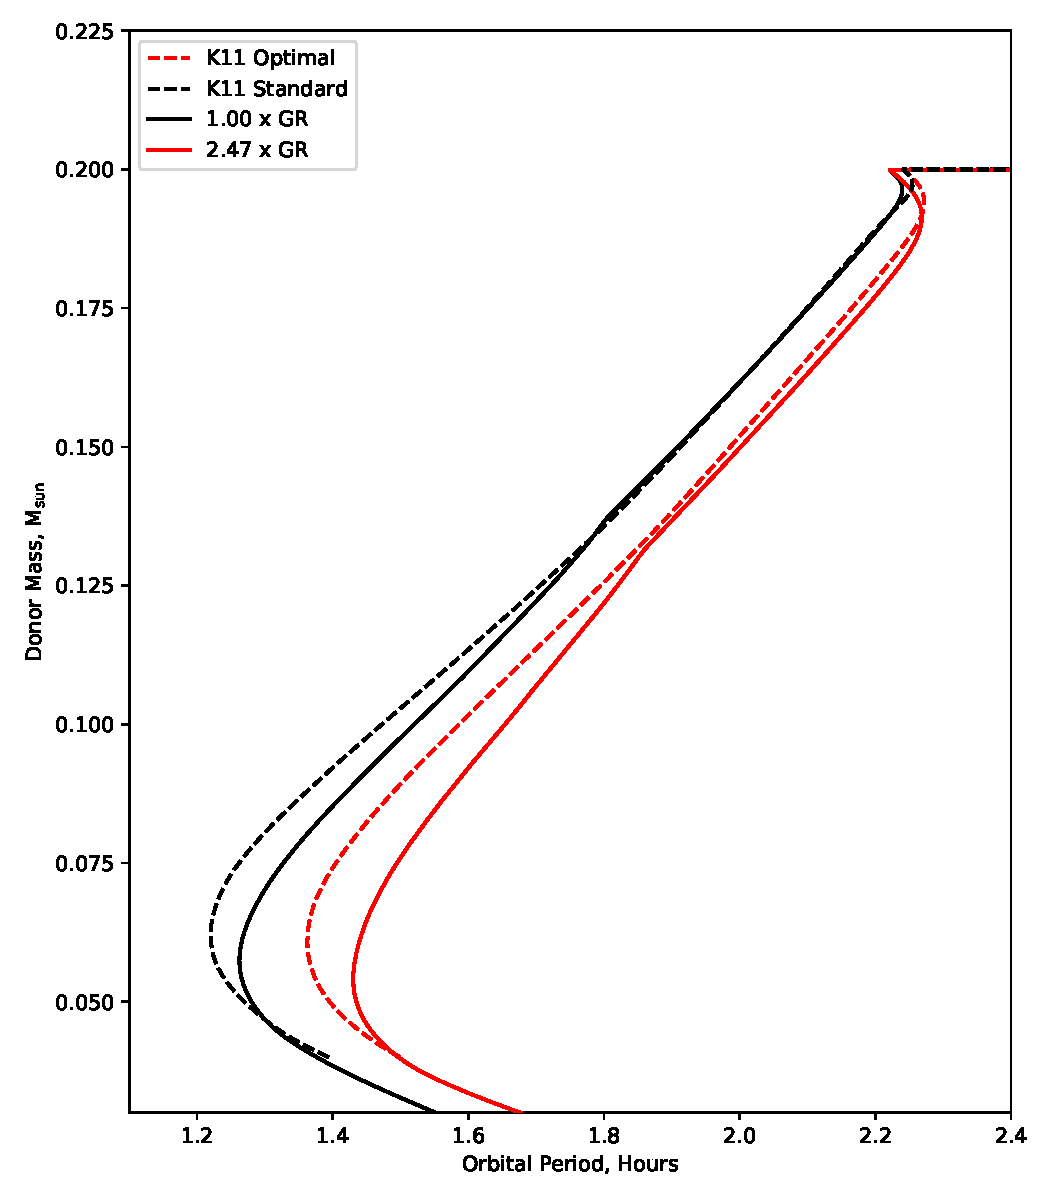
\includegraphics[width=.9\textwidth]{figures/modelling/reproducing_K11_tracks_fspot0.100.pdf}
    \caption{Showing how well MESA can reproduce the canonical \citet{knigge11} donor tracks. {\bf Solid lines} are MESA tracks, and {\bf dotted lines} are the \citet{knigge11} tracks. {\bf Black} lines have only gravitational braking below the period gap, and {\bf red} lines gave gravitational braking at $2.47\times$ strength below the period gap.}
    \label{fig:results:MESA can reproduce the K11 tracks}
\end{figure}


\newpage
\section{For what range of masses can we extract mass loss rates?}
\label{sect:results:MESA massloss allowable mass range}

% This section evaluates the feasibility of using the radius of a star to extract present-day mass loss rates.
Note that the analysis of this section does not include any star spots, i.e. $f_{\rm spot} = 0$ for these models.

Recall from \S\ref{sect:introduction:period minimum and bouncers} the two timescales that govern the response of the donor to mass loss: $\tau_{\rm KH}$ and $\tau_{\dot M}$. These timescales are calculated by
\begin{align}
    \tau_{\rm KH} =& \frac{G M_{\rm donor}^2}{L_{\rm donor} R_{\rm donor}} \\[8pt]
    \tau_{\dot M} =& \frac{\dot M}{M_{\rm donor}}
\end{align}
If $\tau_{\rm KH} \ll \tau_{\dot M}$, the donor is able to maintain thermal equilibrium and is indistinguishable from a singleton star of the same mass.

If $\tau_{\rm KH} \gg \tau_{\dot M}$, the donor is not able to maintain equilibrium, and mass loss is fast and adiabatic.
The donor is inflated by mass loss, but since the stellar structure reacts relatively slowly, the adjustment of the structure towards equilibrium can be interrupted by changes in mass loss rate. This time lag between the star beginning to experience a specific mass loss rate, and the structure adjusting to reflect it makes the degree of inflation of the donor sensitive to the mass loss \textit{history} of the donor.
% The donor is inflated by mass loss, but because the stellar structure as a whole reacts relatively slowly, the effect of past mass loss is retained and the degree of inflation becomes sensitive to the mass loss \textit{history} of the donor.

Calculating the two timescales for CVs reveals that for much of their lives, $\tau_{\rm KH} \sim \tau_{\dot M}$ \citep{knigge11} - meaning that most CV donors are \textit{almost} able to maintain thermal equilibrium, but are still mildly affected by mass loss.
Under this almost-equilibrium regime, mass loss induces some degree of radius inflation in the donor, but because the star adjusts on timescales comparable to $\tau_{\dot M}$, the degree of inflation only depends on the present-day average $\dot M$. In this regime, we can discard the mass loss history of the donor, and use the radius inflation as a diagnostic for the baseline mass loss rate, averaged over $\tau_{\dot M} \sim 1$Gyr.
% This is also the justification for the CV tracks in \S\ref{sect:results:reproducing K11 tracks} to not include the star spot radius correction. As the donor decreases in mass, the necessary spot parameters to correct its radius will change (refer to \S\ref{sect:modelling:tuning star spots to observations}). However, the donor structure would only react to a change in spot parameters on the $\tau_{\rm KH}$ timescale, causing a CV donor model to effectively have the `wrong' spot parameters for its mass, due to the time lag between parameters changing and the donor radius responding to that change.


Whether a donor radius is sensitive to its $\dot M$ history is a function of $M_{\rm donor}$. As $M_{\rm donor}$ falls, $\tau_{\rm KH}$ begins to rise faster than $\tau_{\dot M}$. Figure~\ref{fig:results:how does tauKH and tauMdot vary with donor mass} shows this trend, produced by a MESA model of a CV using the configuration provided in \citet{Paxton_2015}.
The rise in $\tau_{\rm KH}$ relative to $\tau_{\dot M}$ becomes significant at $\sim 0.1 M_\odot$, around the mass the donor enters the adiabatic $\tau_{\rm KH} \gg \tau_{\dot M}$ period bouncer phase c.f.~\S\ref{sect:introduction:period minimum and bouncers}.
\begin{figure}
    \centering
    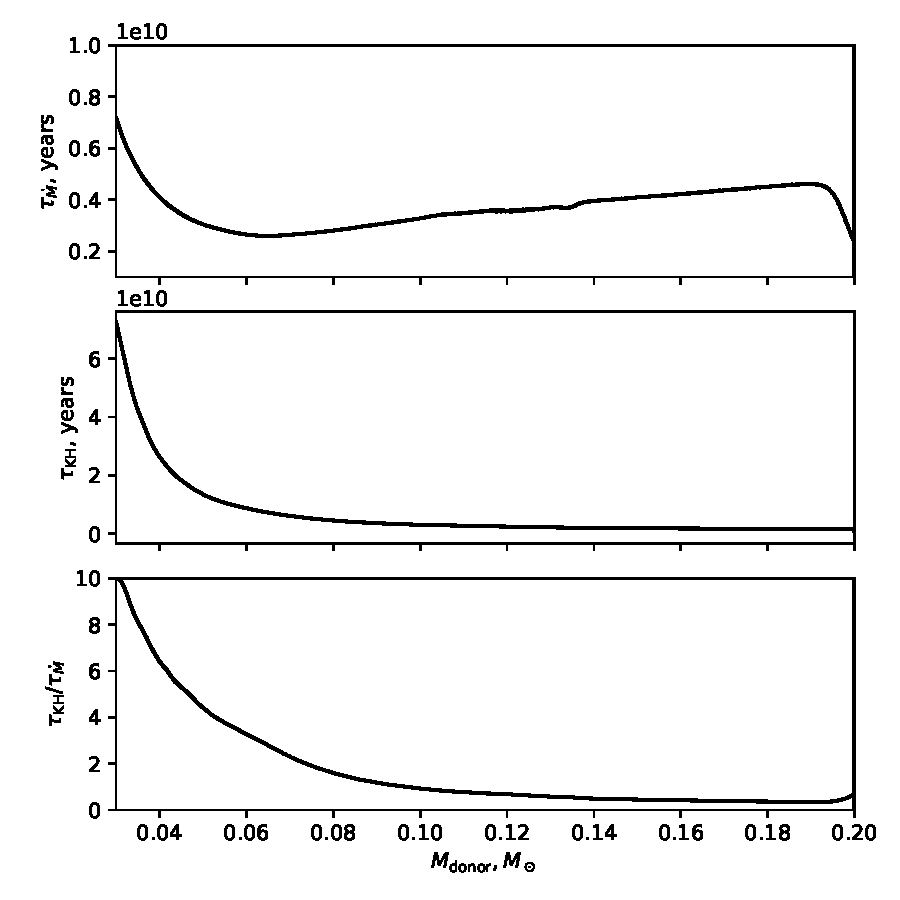
\includegraphics[width=\textwidth]{figures/modelling/tau_both_vs_donor_mass_AML000.pdf}
    \caption{Showing how the two timescales, $\tau_{\rm KH}$ and $\tau_{\dot M}$ vary with donor mass below the period gap in CV donors, as modelled by MESA \citep{Paxton_2015,Pala2017a}.}
    \label{fig:results:how does tauKH and tauMdot vary with donor mass}
\end{figure}

We can determine the range of donor masses for which $\tau_{\rm KH} \sim \tau_{\dot M}$ from MESA models.
First, a series of singleton models (this time using the MESA configuration given in \S\ref{sect:modelling:MESA configs}) were evaluated with varying amounts of fixed mass loss rates, uniformly spaced between $\log (\dot M, M_\odot \mathrm{yr}^{-1}) = -9.9 \rightarrow -10.8$.
Then, a series of MESA CV models were run with gravitational losses amplified by $x = 1 \rightarrow 6$, using the configuration and AML amplification in \S\ref{sect:results:reproducing K11 tracks}.
Finally, each model has its radius, $R$, and $\dot M$ extracted at $0.1 M_\odot$. Since the CV models have varying $\dot M$ and the singleton models do not, if $\dot M$ history does not affect radius inflation the radii between the two sets of models will match, and a disagreement indicates that history plays a significant role in radius inflation.
 Figure~\ref{fig:results:comparing radii at 0.1Msun} shows this, and little divergence between the two sets of radii is visible. Note that higher $\dot M$ show a small but increasing degree of divergence, as we might expect since higher $\dot M$ corresponds to lower $\tau_{\dot M}$.
\begin{figure}
    \centering
    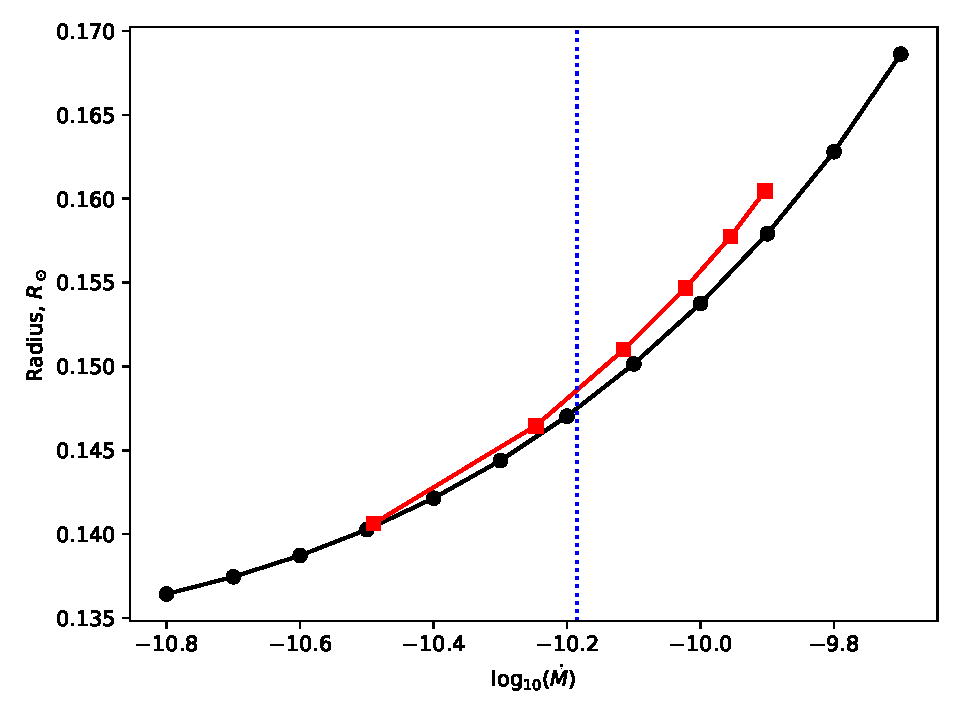
\includegraphics[width=.8\textwidth]{figures/modelling/compare_0.1Msun_with_CV_track_K11_fig1.pdf}
    \caption{Showing the radius and mass loss extracted from MESA models at $0.1 M_\odot$. The {\bf black} line is a series of singleton models with constant mass loss, and the {\bf red} line is a series of CV models with gravitational AML amplified by $x = 1 \rightarrow 6$, with the lowest AML rate on the left. The {\bf blue dotted line} shows $\dot M$ for a CV with $2.47\times$ gravitational braking strength as predicted by a MESA CV model.}
    \label{fig:results:comparing radii at 0.1Msun}
\end{figure}

Now, by looking at what level of divergence historical changes in $\dot M$ induces at various donor masses, we can evaluate what mass range is acceptable.
By instead plotting the difference between the two sets of models, and repeating the same process for a range of masses, Figure~\ref{fig:results:comparing radii over a range of masses} is produced.
The upper limit on mass must be $0.2 M_\odot$, as this is the enforced mass of the period gap, and for a lower limit I impose an acceptable level of disagreement of $3\%$. It can be seen that the minimum acceptable mass is then $0.08 M_\odot$.
\begin{figure}
    \centering
    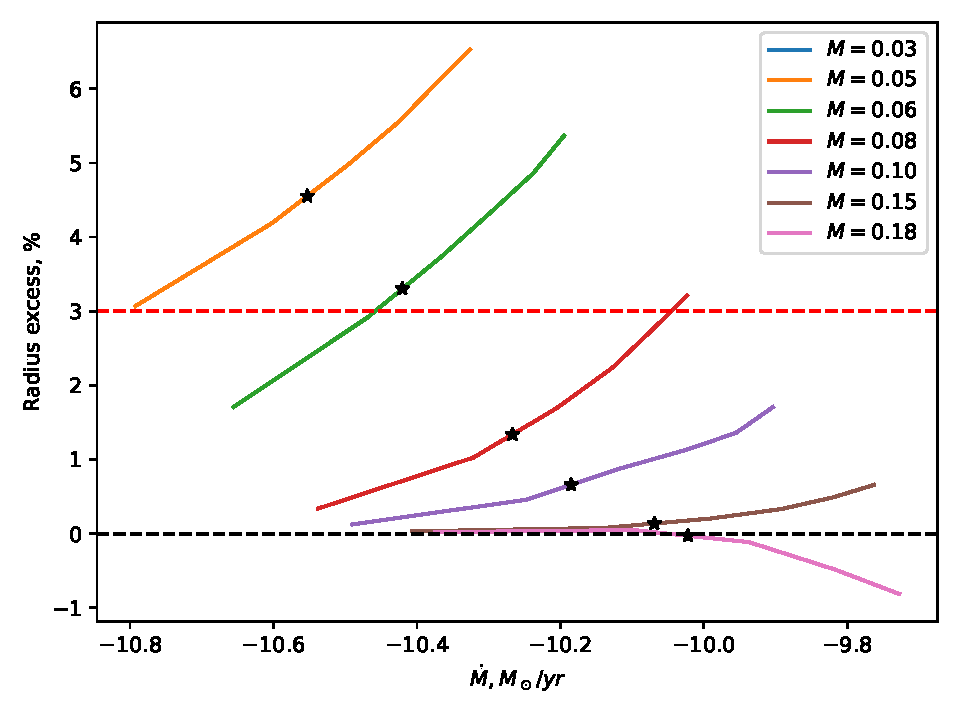
\includegraphics[width=\textwidth]{figures/modelling/compare_multiple_mass_with_CV_K11_fig1a.pdf}
    \caption{The inflation of CV model radii, $R_{CV}$ (whose $\dot M$ is time-dependent), over singleton model radii, $R_S$ (whose $\dot M$ is constant), from Figure~\ref{fig:results:comparing radii at 0.1Msun}, for a range of masses. The {\bf stars} on each line show the $\dot M$ and inflation for a model with gravitational braking at $2.47\times$ strength, mirroring the \citet{knigge11} optimal track. The {\bf red dashed line} shows the upper limit for acceptable disagreement, and the {\bf black dashed line} shows perfect agreement.}
    \label{fig:results:comparing radii over a range of masses}
\end{figure}


\newpage
\section{Tuning star spot parameters to observations}
\label{sect:modelling:tuning star spots to observations}

With star spots implemented in MESA in \S\ref{sect:modelling:starspots in MESA}, the Brown relation can now be reproduced.
For simplicity, $x_{\rm spot}$ is fixed at 0 and $f_{\rm spot}$ is varied.
Since radius increases monotonically with $f_{\rm spot}$, a binary chop is performed (see \S\ref{sect:modelling:binary chop methodology}), optimising for $\Delta R=R_{\rm MESA}-(1.045\times R_{\rm Brown})=0$ at a stellar age of 2~Gyrs for a range of masses. The 4.5\% radius increase is to compensate for the non-spherical Roche geometry of the donor, c.f. \citet{knigge11}.
The resulting M-$f_{\rm spot}$ relation is shown in Figure~\ref{fig:modelling:fspot mass relationship}.

Below masses of $\sim 0.12 M_\odot$, the required $f_{\rm spot}$ becomes slightly negative, i.e. default MESA models are larger than observations plus the $4.5\%$ non-spherical correction.
Since a negative coverage fraction is unphysical, negative values of $f_{\rm spot}$ are set equal to 0 and it should be emphasised that derived mass loss rates may become somewhat unreliable below this mass.
% Below $M_{\rm donor} = 0.121 M_\odot$ the Brown relation transitions to the \citet{baraffe2015} theoretical tracks, so model agreement is perhaps unsurprising here.
However, the clear trend in $f_{\rm spot}$ towards 0 prior to this, and the close proximity to $f_{\rm spot} = 0$ below $0.12 M_\odot$ suggests that the MESA radius calibration given here is still valid.
% The severity of this unreliability is not catastrophic, as the minimum value of $f_{\rm spot}$ is still reasonably close to 0.

There is significant scatter in the Brown mass-radius relation, that is not captured in these models. The inherent scatter in radius for the observations is $\sim 3\%$ between 0.1 and 0.2 $M_\odot$, which adds to the uncertainty in modelled radius inflation, and thus mass loss rate. Below $\sim 0.1 M_\odot$, the scatter is not able to be characterised.
Whilst this may skew an individual system, on average the inferred mass loss from model radius should be accurate. Therefore, this effect should not corrupt the $\dot M$ results with a large enough sample size.
Since the uncertainties I report here do not include the effects of the scatter in the Brown mass-radius relation, they are underestimates of the true uncertainty. However, due to the very poor constraints on the scatter, this effect is ignored until more information is available.

\begin{figure}
    \centering
    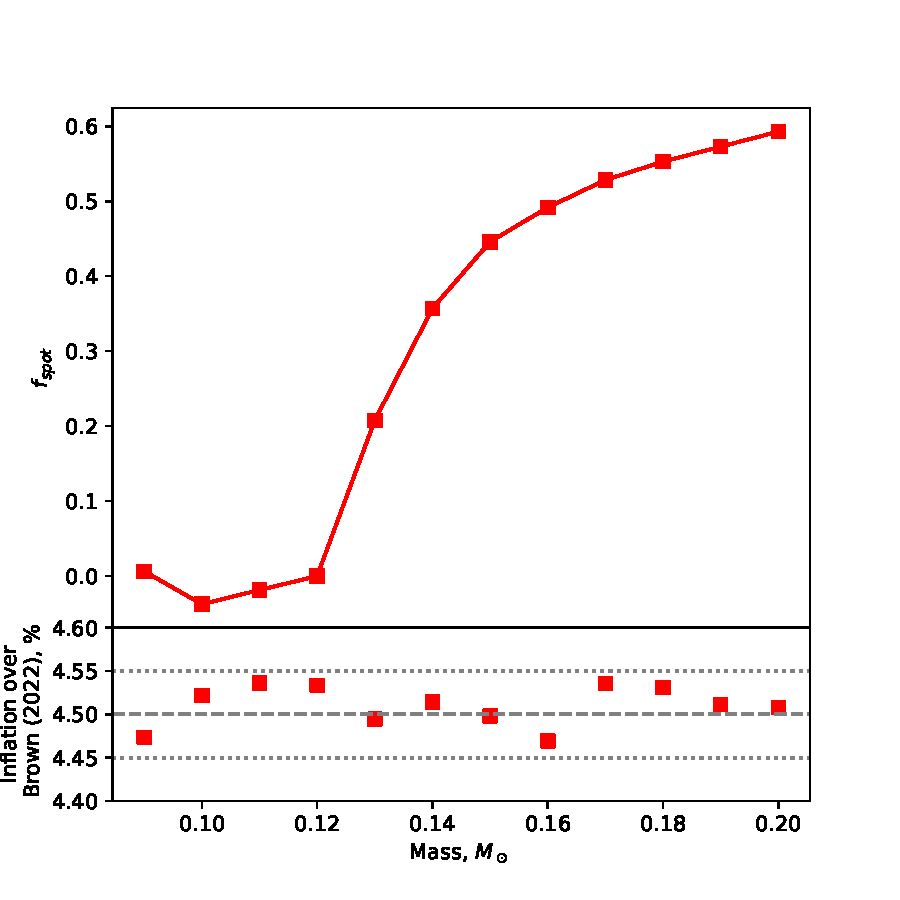
\includegraphics[width=\textwidth]{figures/modelling/fspot_relation_to_match_brown_plus_4.5.pdf}
    \caption{{\it Top}: The required $f_{\rm spot}$ that is applied to tune M dwarf MESA models to match the Brown relation, plus an added $4.5\%$ inflation due to non-spherical Roche geometry. {\it Bottom}: the residuals from the best fit value of $f_{\rm spot}$. The {\bf dotted lines} show the acceptable deviation from perfect agreement in order to terminate the binary chop, and the {\bf dashed line} shows the target inflation. Note that when finding the necessary value of $f_{\rm spot}$ to match the Brown relation $x_{\rm spot} \equiv 0$, and negative values of $f_{\rm spot}$ were allowed. However, in all subsequent modelling, negative $f_{\rm spot}$ were set to 0. {\bf Red squares} show evaluated MESA models.}
    \label{fig:modelling:fspot mass relationship}
\end{figure}



\section{Inferred mass and angular momentum loss rates from CV donors}
\label{sect:modelling:donor mass loss rates}

Overall, there are 33 systems with eclipse-modelled characterisations available with donors in the correct mass range of $0.08 M_\odot < M_{\rm donor} < 0.20 M_\odot$, catalogued in Table~\ref{table:results:mdot modelling}.

Table~\ref{table:results:Jdot results} shows the AML rates, $\dot J$, calculated using Equation~\ref{eqn:modelling:Jdot from Mdot} for the systems for which $\dot M$ could be calculated from donor properties. Also shown is the AML expected from gravitational losses alone for that system, and the ratio between the observed and expected values.

Two systems appear to have less AML than is predicted by gravitational losses: ASASSN-17fo (from Chapter~\ref{chpt:characterisation of 12 new CVs}) and SDSS J0903 \citep{Savoury2011}, and an erroneous eclipse model result can be eliminated in each case.
ASASSN-17fo is confidently eclipse modelled, with distinct, well modelled eclipse features and a good white dwarf flux fit, so is unlikely to be unreliable. SDSS J0903 also has a confident eclipse model fit. Whilst the bright spot features of this system are less distinct, the fitting results are satisfactory.
However, the inferred $\dot M$ is contingent on a chain of assumptions all holding true; the eclipse modelling must be robust, the MESA configuration must be accurate \textit{for the specific donor being considered}, and the equilibrium radius of the donor in question must be well-described by the Brown relation. A failure in any of these steps will produce incorrect values of $\dot M$ and $\dot J$, and the consequences of the breakdown of these assumptions is discussed in \S\ref{sect:massloss and AML:systematic bias}.

Aside from these two cases the inferred $\dot M$ are generally physically reasonable, suggesting that the general data set is acceptable for preliminary analysis. In the interests of honest analysis, the two sub-gravitational loss CVs are still included in the following examination of the data.


\begin{table*}
    \centering
    \caption{The inferred $\dot M$ for eclipse-modelled CVs. For the Source column, `W22' are from Chapter~\ref{chpt:characterisation of 12 new CVs}, `M19' are systems modelled by \citet{McAllister2019}, `M17b' is from \citet{mcallister2017b}, `S11' are from \citet{Savoury2011}}
    \label{table:results:mdot modelling}
    \begin{tabular}{llccc}
        \hline \\
        {\bf System Name:} & \textbf{Source} & \textbf{$M_{\rm donor}, M_\odot$}  & \textbf{$R_{\rm donor}, R_\odot$}  & \textbf{$\log_{10}(\dot M,\ M_\odot / {\rm yr})$} \\
        \hline \hline \\
        ASASSN-14hq         &  W22      & $0.097 \pm 0.002$ & $0.157 \pm 0.001$ & $ -9.897 \pm 0.008$ \\
        ASASSN-15pb         &  W22      & $0.148 \pm 0.008$ & $0.209 \pm 0.003$ & $ -9.997 \pm 0.164$ \\
        ASASSN-17fo         &  W22      & $0.109 \pm 0.001$ & $0.144 \pm 0.001$ & $-10.859 \pm 0.137$ \\
        AY For              &  W22      & $0.106 \pm 0.005$ & $0.162 \pm 0.002$ & $ -9.918 \pm 0.024$ \\
        CSS090419           &  W22      & $0.087 \pm 0.016$ & $0.152 \pm 0.006$ & $ -9.859 \pm 0.003$ \\
        CSS090622           &  W22      & $0.105 \pm 0.009$ & $0.155 \pm 0.004$ & $-10.046 \pm 0.074$ \\
        MASTER OT J0014     &  W22      & $0.123 \pm 0.006$ & $0.165 \pm 0.002$ & $-10.279 \pm 0.328$ \\
        OGLE82              &  W22      & $0.132 \pm 0.003$ & $0.170 \pm 0.001$ & $-11.686 \pm 1.078$ \\
        SDSS J0748          &  W22      & $0.085 \pm 0.010$ & $0.128 \pm 0.005$ & $-10.438 \pm 0.152$ \\
        SDSS J1524          &  W22      & $0.097 \pm 0.003$ & $0.144 \pm 0.001$ & $-10.210 \pm 0.030$ \\
        CSS080623           &  M19      & $0.081 \pm 0.005$ & $0.128 \pm 0.002$ & $-10.343 \pm 0.041$ \\
        CSS110113           &  M19      & $0.105 \pm 0.007$ & $0.149 \pm 0.003$ & $-10.272 \pm 0.129$ \\
        OY Car              &  M19      & $0.093 \pm 0.004$ & $0.139 \pm 0.001$ & $-10.278 \pm 0.046$ \\
        SDSS J0901          &  M19      & $0.138 \pm 0.007$ & $0.182 \pm 0.003$ & $-10.547 \pm 0.368$ \\
        SDSS J1152          &  M19      & $0.094 \pm 0.016$ & $0.147 \pm 0.006$ & $-10.062 \pm 0.156$ \\
        SSS100615           &  M19      & $0.083 \pm 0.005$ & $0.128 \pm 0.002$ & $-10.384 \pm 0.038$ \\
        ASASSN-14ag         &  M17b     & $0.093 \pm 0.010$ & $0.135 \pm 0.007$ & $-10.416 \pm 0.211$ \\
        CTCV J2354-4700     &  S11      & $0.101 \pm 0.003$ & $0.146 \pm 0.001$ & $-10.245 \pm 0.030$ \\
        % SDSS J1152          &  S11      & $0.087 \pm 0.006$ & $0.142 \pm 0.003$ & $-10.068 \pm 0.025$ \\
        OU Vir              &  S11      & $0.116 \pm 0.002$ & $0.163 \pm 0.001$ & $-10.067 \pm 0.026$ \\
        XZ Eri              &  S11      & $0.091 \pm 0.004$ & $0.135 \pm 0.001$ & $-10.352 \pm 0.054$ \\
        SDSS J0903          &  S11      & $0.099 \pm 0.004$ & $0.136 \pm 0.002$ & $-10.677 \pm 0.155$ \\
        SDSS J1227          &  S11      & $0.089 \pm 0.002$ & $0.137 \pm 0.001$ & $-10.243 \pm 0.017$ \\
        SDSS J1502          &  S11      & $0.078 \pm 0.001$ & $0.124 \pm 0.001$ & $-10.377 \pm 0.008$ \\
        ASASSN-14kb         &  W22      & $0.134 \pm 0.003$ & $0.164 \pm 0.001$ & -                   \\
        CTCV 1300-3052      &  M19      & $0.166 \pm 0.006$ & $0.211 \pm 0.002$ & -                   \\
        DV UMa              &  M19      & $0.187 \pm 0.012$ & $0.215 \pm 0.005$ & -                   \\
        IY UMa              &  M19      & $0.141 \pm 0.007$ & $0.177 \pm 0.002$ & -                   \\
        SSS130413           &  M19      & $0.140 \pm 0.012$ & $0.163 \pm 0.004$ & -                   \\
        V713 Cep            &  M19      & $0.176 \pm 0.018$ & $0.208 \pm 0.005$ & -                   \\
        Z Cha               &  M19      & $0.152 \pm 0.005$ & $0.182 \pm 0.002$ & -                   \\
        CTCV J1300-3052     &  S11      & $0.177 \pm 0.021$ & $0.215 \pm 0.008$ & -                   \\
        DV UMa              &  S11      & $0.196 \pm 0.005$ & $0.218 \pm 0.001$ & -                   \\
        % CSS090102           &  W22      & $0.059 \pm 0.003$ & $0.119 \pm 0.002$ & $-10.255 \pm 0.024$ \\
        % ASASSN-16kr         &  W20      & $0.042 \pm 0.003$ & $0.106 \pm 0.002$ & $-10.672 \pm 0.274$ \\
        % SSSJ1502-3505       &  W20      & $0.042 \pm 0.003$ & $0.106 \pm 0.003$ & $-10.648 \pm 0.206$ \\
        % SDSS 1501           &  M19      & $0.061 \pm 0.004$ & $0.113 \pm 0.002$ & $-10.456 \pm 0.034$ \\
        % SDSS J1057+2759     &  M17a     & $0.044 \pm 0.002$ & $0.109 \pm 0.001$ & $-10.514 \pm 0.102$ \\
        % PHL 1445            &  M15      & $0.064 \pm 0.005$ & $0.109 \pm 0.004$ & $-10.660 \pm 0.101$ \\
        % SDSS 1035           &  S11      & $0.048 \pm 0.001$ & $0.105 \pm 0.001$ & $-10.742 \pm 0.011$ \\
        % SDSS J1501          &  S11      & $0.077 \pm 0.010$ & $0.122 \pm 0.005$ & $-10.429 \pm 0.066$ \\
        % ASASSN-17jf         &  W20      & $0.060 \pm 0.008$ & $0.112 \pm 0.004$ & -                   \\
        % GY Cnc              &  M19      & $0.394 \pm 0.022$ & $0.446 \pm 0.009$ & -                   \\
        % SDSS 1006           &  M19      & $0.370 \pm 0.060$ & $0.457 \pm 0.026$ & -                   \\
        % SDSS 1702           &  S11      & $0.223 \pm 0.010$ & $0.252 \pm 0.004$ & -                   \\
        % SDSS 1507           &  S11      & $0.058 \pm 0.002$ & $0.097 \pm 0.001$ & -                   \\
        % SDSS 1433           &  S11      & $0.057 \pm 0.001$ & $0.107 \pm 0.001$ & -                   \\
        % IP Peg              &  C10      & $0.550 \pm 0.020$ & $0.466 \pm 0.006$ & -                   \\
        \hline
    \end{tabular}
\end{table*}

\begin{table*}
    \centering
    \caption{The inferred AML rates for the CVs in this sample. $\dot J_{\rm total}$ is calculated from the inferred $\dot M$, and $\dot J_{\rm GR}$ is the calculated gravitational AML rate. Sources are keyed the same as Table~\ref{table:results:mdot modelling}.}
    \label{table:results:Jdot results}
    \begin{tabular}{llccc}
        \hline
        {\bf System Name:} & \textbf{Source}  & \textbf{$\log(\dot J_{\rm total}, J)$} & \textbf{$\log(\dot J_{\rm GR}, J)$} & \textbf{$\dot J_{\rm total} / \dot J_{\rm GR}$} \\
        \hline \hline
        ASASSN-14hq     &  W22      & $27.157 \pm 0.009$    & $26.681 \pm 0.007$    & $2.996 \pm 0.081$ \\
        ASASSN-15pb     &  W22      & $27.091 \pm 0.162$    & $26.796 \pm 0.013$    & $2.115 \pm 0.818$ \\
        ASASSN-17fo     &  W22      & $26.240 \pm 0.137$    & $26.711 \pm 0.004$    & $0.355 \pm 0.114$ \\
        AY For          &  W22      & $27.184 \pm 0.026$    & $26.705 \pm 0.015$    & $3.021 \pm 0.204$ \\
        CSS090419       &  W22      & $27.158 \pm 0.039$    & $26.634 \pm 0.058$    & $3.381 \pm 0.548$ \\
        CSS090622       &  W22      & $26.994 \pm 0.078$    & $26.699 \pm 0.028$    & $2.011 \pm 0.388$ \\
        MASTER OT J0014 &  W22      & $26.842 \pm 0.325$    & $26.745 \pm 0.014$    & $1.661 \pm 1.488$ \\
        OGLE82          &  W22      & $25.428 \pm 1.083$    & $26.767 \pm 0.009$    & $0.980 \pm 8.280$ \\
        SDSS J0748      &  W22      & $26.645 \pm 0.156$    & $26.629 \pm 0.053$    & $1.116 \pm 0.442$ \\
        SDSS J1524      &  W22      & $27.027 \pm 0.031$    & $26.723 \pm 0.043$    & $2.027 \pm 0.234$ \\
        CSS080623       &  M19      & $26.705 \pm 0.042$    & $26.615 \pm 0.026$    & $1.238 \pm 0.141$ \\
        CSS110113       &  M19      & $26.895 \pm 0.128$    & $26.701 \pm 0.019$    & $1.633 \pm 0.502$ \\
        OY Car          &  M19      & $26.844 \pm 0.046$    & $26.666 \pm 0.014$    & $1.517 \pm 0.168$ \\
        SDSS J0901      &  M19      & $26.536 \pm 0.368$    & $26.780 \pm 0.014$    & $0.815 \pm 0.870$ \\
        SDSS J1152      &  M19      & $26.954 \pm 0.157$    & $26.656 \pm 0.073$    & $2.149 \pm 0.894$ \\
        SSS100615       &  M19      & $26.730 \pm 0.039$    & $26.625 \pm 0.024$    & $1.282 \pm 0.138$ \\
        ASASSN-14ag     &  M17b     & $26.587 \pm 0.215$    & $26.657 \pm 0.056$    & $0.968 \pm 0.526$ \\
        CTCV J2354-4700 &  S11      & $26.899 \pm 0.032$    & $26.691 \pm 0.008$    & $1.616 \pm 0.122$ \\
        % SDSS J1152      &  S11      & $26.917 \pm 0.030$    & $26.642 \pm 0.026$    & $1.893 \pm 0.172$ \\
        OU Vir          &  S11      & $26.992 \pm 0.027$    & $26.729 \pm 0.005$    & $1.837 \pm 0.117$ \\
        XZ Eri          &  S11      & $26.721 \pm 0.054$    & $26.659 \pm 0.015$    & $1.164 \pm 0.151$ \\
        SDSS J0903      &  S11      & $26.427 \pm 0.154$    & $26.685 \pm 0.012$    & $0.587 \pm 0.217$ \\
        SDSS J1227      &  S11      & $26.848 \pm 0.018$    & $26.652 \pm 0.010$    & $1.572 \pm 0.075$ \\
        SDSS J1502      &  S11      & $26.669 \pm 0.009$    & $26.602 \pm 0.005$    & $1.169 \pm 0.026$ \\
        % CSS090102       &  W22      & $26.768 \pm 0.027$    & $26.422 \pm 0.046$    & $2.235 \pm 0.273$ \\
        % ASASSN-16kr     &  W20      & $26.490 \pm 0.276$    & $26.059 \pm 0.093$    & $3.375 \pm 2.522$ \\
        % SSSJ1502-3505   &  W20      & $26.446 \pm 0.209$    & $26.070 \pm 0.103$    & $2.737 \pm 1.564$ \\
        % SDSS 1501       &  M19      & $26.600 \pm 0.035$    & $26.448 \pm 0.052$    & $1.435 \pm 0.210$ \\
        % SDSS J1057      &  M17a     & $26.598 \pm 0.103$    & $26.109 \pm 0.056$    & $3.203 \pm 0.874$ \\
        % PHL 1445        &  M15      & $26.386 \pm 0.101$    & $26.482 \pm 0.057$    & $0.830 \pm 0.226$ \\
        % SDSS 1035       &  S11      & $26.365 \pm 0.011$    & $26.212 \pm 0.029$    & $1.426 \pm 0.101$ \\
        % SDSS 1501       &  S11      & $26.639 \pm 0.067$    & $26.581 \pm 0.072$    & $1.169 \pm 0.271$ \\
        % ASASSN-14kb     &  W22      & $   NaN \pm   NaN$    & $26.772 \pm 0.009$    & $  NaN \pm   NaN$ \\
        % ASASSN-17jf     &  W20      & $   NaN \pm   NaN$    & $26.416 \pm 0.127$    & $  NaN \pm   NaN$ \\
        % CTCV 1300-3052  &  M19      & $   NaN \pm   NaN$    & $26.821 \pm 0.008$    & $  NaN \pm   NaN$ \\
        % DV UMa          &  M19      & $   NaN \pm   NaN$    & $27.036 \pm 0.463$    & $  NaN \pm   NaN$ \\
        % GY Cnc          &  M19      & $   NaN \pm   NaN$    & $28.717 \pm 0.053$    & $  NaN \pm   NaN$ \\
        % IY UMa          &  M19      & $   NaN \pm   NaN$    & $26.785 \pm 0.013$    & $  NaN \pm   NaN$ \\
        % SDSS 1006       &  M19      & $   NaN \pm   NaN$    & $28.647 \pm 0.179$    & $  NaN \pm   NaN$ \\
        % SSS130413       &  M19      & $   NaN \pm   NaN$    & $26.781 \pm 0.023$    & $  NaN \pm   NaN$ \\
        % V713 Cep        &  M19      & $   NaN \pm   NaN$    & $26.953 \pm 0.388$    & $  NaN \pm   NaN$ \\
        % Z Cha           &  M19      & $   NaN \pm   NaN$    & $26.803 \pm 0.007$    & $  NaN \pm   NaN$ \\
        % CTCV J1300-3052 &  S11      & $   NaN \pm   NaN$    & $27.023 \pm 0.476$    & $  NaN \pm   NaN$ \\
        % DV UMa          &  S11      & $   NaN \pm   NaN$    & $27.142 \pm 0.530$    & $  NaN \pm   NaN$ \\
        % SDSS 1702       &  S11      & $   NaN \pm   NaN$    & $28.218 \pm 0.140$    & $  NaN \pm   NaN$ \\
        % SDSS 1507       &  S11      & $   NaN \pm   NaN$    & $26.402 \pm 0.030$    & $  NaN \pm   NaN$ \\
        % SDSS 1433       &  S11      & $   NaN \pm   NaN$    & $26.399 \pm 0.011$    & $  NaN \pm   NaN$ \\
        % IP Peg          &  C10      & $   NaN \pm   NaN$    & $29.061 \pm 0.034$    & $  NaN \pm   NaN$ \\
        \hline
    \end{tabular}
\end{table*}


\subsection{Systematic issues with mass loss estimation}
\label{sect:massloss and AML:systematic bias}

It is critical to treat these mass loss rates with caution.
The sample as given here is subject to systematic bias as a result of the sparse nature of the data used to calibrate the Brown relation, and the validity of $\dot M$ and $\dot J$ is sensitive to the validity of the MESA configuration for the donor model.
Whilst the majority of CV donors are probably well-described by my MESA configuration, we cannot assume that \textit{all} donors will be; the configuration could easily be invalidated by, for example, the presence of a more evolved donor, or one with a substantially different metallicity from typical M dwarfs.
This would alter the mass-radius exponent of the donor ($\zeta$ in Equation~\ref{eqn:modelling:Jdot from Mdot}) and corrupt the inferred $\dot J$.

Beyond a potentially incorrect MESA configuration, there is a more serious problem with the unknown scatter in the Brown relation.
Consider a star which lies below the Brown relation, i.e. one with a smaller zero-$\dot M$ radius than its mass suggests. If this star begins to experience mass loss, and we measure its radius to be inflated beyond the Brown relation (after factoring for Roche geometry), the corresponding mass loss rate we would find will be \textit{lower} than reality, as some amount of the star's inflation -- the amount required to inflate it to agree with the Brown relation -- is ignored.
This is illustrated in Figure~\ref{fig:massloss and AML:brown scatter causes bias}.
This will also cause some stars to fail to have $\dot M$ inferred. If the zero-$\dot M$ radius is small enough, it becomes likely that the amount of inflation induced by mass loss is not sufficient to bring the star up to the radius assumed by the Brown relation. Such a donor would not be possible to reproduce using this methodology, and 9 such donors (approximately a quarter of the sample) are seen in Table~\ref{table:results:mdot modelling}.
\begin{figure}
    \centering
    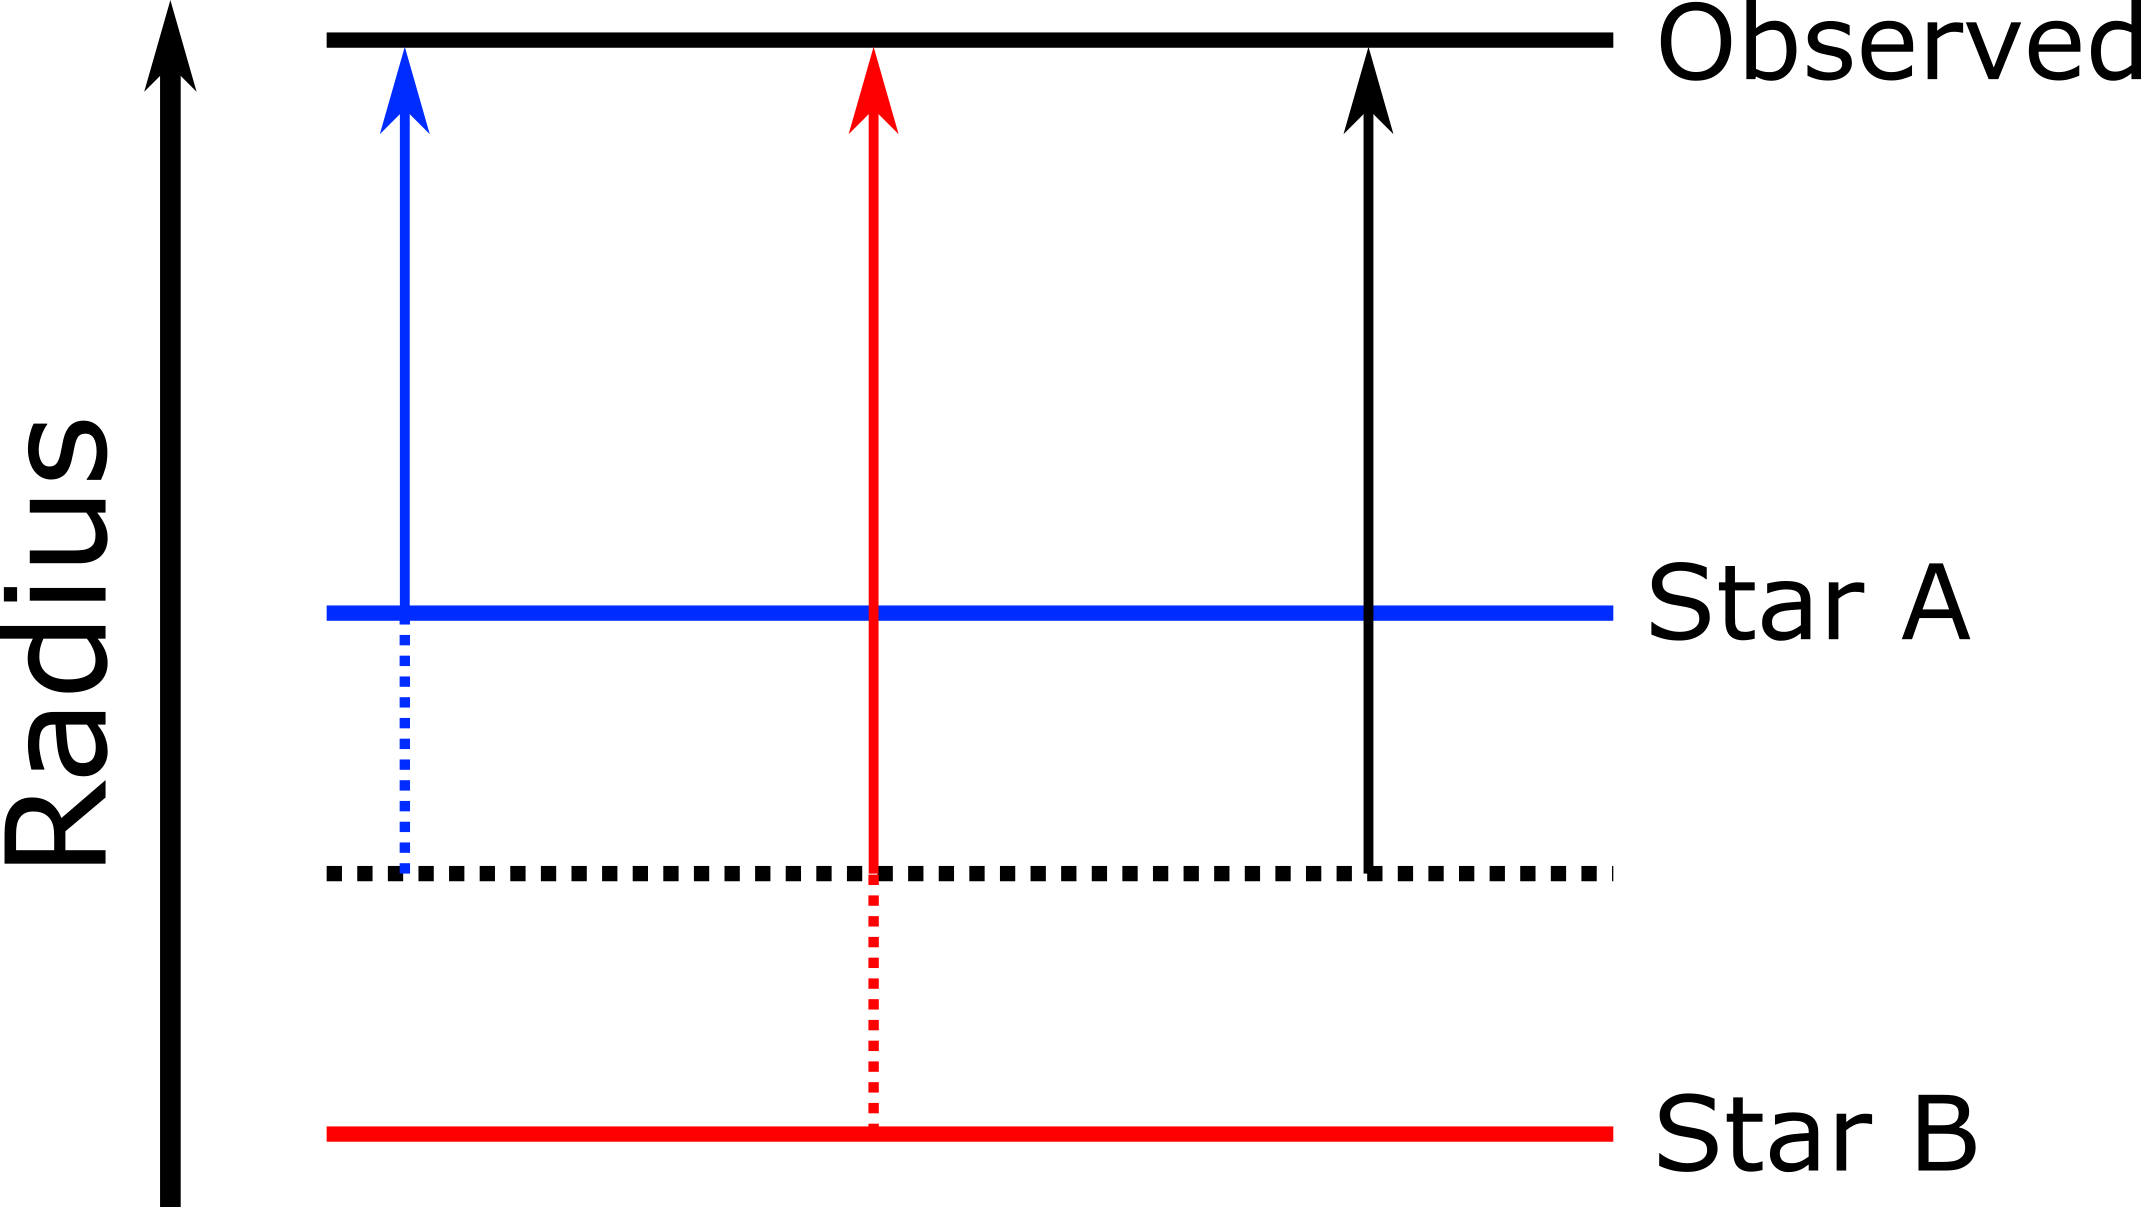
\includegraphics[width=.7\textwidth]{figures/results/brown_scatter_causes_bias.png}
    \caption{Illustrating how scatter about the Brown relation can corrupt inferred $\dot M$ rates. The upper solid black line shows the observed radius of a donor, and the lower three lines show possible zero $\dot M$ radii. The dotted black line shows the radius predicted by the Brown relation. The arrows show the amount of inflation induced by $\dot M$, with longer arrows requiring more $\dot M$. The black arrow shows the reported value, but assumes the donor would exactly agree with the Brown relation. If the zero-$\dot M$ radius of a donor corresponds to star A (blue line), some extra $\dot M$ will be incorrectly attributed to the system (shown as the dotted section). If the zero-$\dot M$ radius of the donor corresponds to star B (red line), some amount of $\dot M$ will be ignored (again shown as the dotted section).}
    \label{fig:massloss and AML:brown scatter causes bias}
\end{figure}

The combination of these two effects makes our dataset as a whole systematically over-estimate $\dot M$. This is because systems with donors that scatter below the Brown relation are preferentially removed from the sample -- they are more likely to have inflations that lie below the baseline radius (i.e. they lie below the dotted black line in Figure~\ref{fig:massloss and AML:brown scatter causes bias}), and are systems which would have had their $\dot M$ under-estimated.
Donors which scatter above the Brown relation are not removed in this way, so over-estimated $\dot M$ become over-represented in the sample.
Some portion of systems are, for the same reasons, reported with abnormally low $\dot M$ -- i.e. ASASSN-17fo and SDSS J0903 -- as their donors scatter below the Brown relation, but not by enough as to remove them from the sample.
Finally, since our reported $\dot M$ do not consider the intrinsic scatter in the M dwarf population, the uncertainties in $\dot M$ reported are likely to be significantly under-estimated.

Although this bias presents a problem for quantitative analysis, the general trends that these data show can still be considered generally correct, with the caveat that these are preliminary results. A larger sample of M dwarf masses and radii in the $M < 0.2 M_\odot$ range to give a better mass-radius relationship is highly desirable, and is likely to be provided in the near future with the release of Gaia DR3.
With a proper characterisation of the intrinsic population scatter, it will be possible to marginalise over the scatter to remove the over-estimation of $\dot M$, more faithfully report uncertainties, and perform more rigorous quantitative analysis of the data.



\section{Mass loss from white dwarf properties}
\label{sect:modelling:white dwarf mass loss rates}

% The characterised CVs also have the white dwarf temperature constrained to within $\sim 2000 \rm K$, allowing the short-term mass loss rate to also be inferred as suggested in \S\ref{sect:modelling:mdot from wd temperature}.
% Note that, despite the large uncertainty in $T_{\rm eff}$, the errors are smaller than those obtained with the donor properties.
% Figure~\todo{Get this figure} compares the $\dot M$ found by each technique, plotted as a function of donor mass.


The white dwarf temperature also reveals information on the mass transfer rate, and the following summary is described more quantitatively by \citet{townsley2009}.
In brief, as accreted material strikes the surface of the white dwarf its kinetic energy is converted to thermal energy, heating the white dwarf surface.
The degree of this heating is related to the rate at which material falls to the surface -- if more material falls in, more heating is induced.
Since, in general, we can assume that the rate material falls onto the white dwarf is roughly equal to the rate at which material enters the accretion disc from the donor, the white dwarf $T_{\rm eff}$ becomes a proxy diagnostic of the donor $\dot M$.
Simulations demonstrate that even through successive Nova eruptions, the core temperature of the white dwarf is stable over timescales of $\sim 10^8$ years \citep{epelstain2007}, so if the accretion rate falls, the white dwarf $T_{\rm eff}$ is able to cool to the appropriate, lower temperature and remain accurate to the present-day accretion rate.

The white dwarf temperature approach holds a major advantage over using the donor properties: measurements of white dwarf temperatures are easier to gather in large sample sizes.
However, the white dwarf temperature is capable of responding to changes in $\dot M$ on $\tau_{\rm Twd} \sim 10^3 - 10^5\ {\rm yrs}$ \citep{townsley2009}, as opposed to the $\rm \sim~Gyr$ timescales of the donor-based method described in \S\ref{sect:modelling:donor mass loss rates}, thus the $\dot M$ inferred from the white dwarf is averaged over $\tau_{\rm Twd}$ and only provides a short-term snapshot of the $\dot M$ and is susceptible to corruption from outbursts.
% In addition, the method assumes that the white dwarf is not a helium-core white dwarf, which is not always the case in the CV population and introduces significant unmodelled scatter to the results.

The short-term average mass loss rate, $\langle\dot M\rangle$, is ultimately a function only of white dwarf mass, and temperature, given in Equation~\ref{eqn:modelling:Mdot from wd temperature}.
\begin{equation}
    \label{eqn:modelling:Mdot from wd temperature}
    T_{\rm eff} = 1.7 \times 10^4 {\rm K} \bigg( \frac{\langle\dot M\rangle}{10^{-10} M_\odot {\rm yr}^{-1}} \bigg)^{1/4} \bigg( \frac{M_{\rm wd}}{0.9 M_\odot} \bigg)
\end{equation}

Recently, \citet{Pala2021} used spectroscopically estimated $T_{\rm eff}$ and $M_{\rm wd}$ to infer the $\dot M$ of 65 CVs. %, the result of which is reproduced in Figure~\ref{fig:modelling:pala2022 fig13}.
One finding from this analysis was an inverse correlation between $M_{\rm wd}$ and $\dot M$, contrary to the prediction of gravitational wave braking that lower mass systems should have lower AML rates driving lower $\dot M$.
As the eclipse modelling of CVs also produces a measure of $T_{\rm eff}$, the systems analysed for this thesis can be processed with {\it both} techniques, and have their results compared. Table~\ref{table:results:Mdot from white dwarf parameters} shows the resulting $\dot M$ from the white dwarf parameters.
% \begin{figure}
%     \centering
%     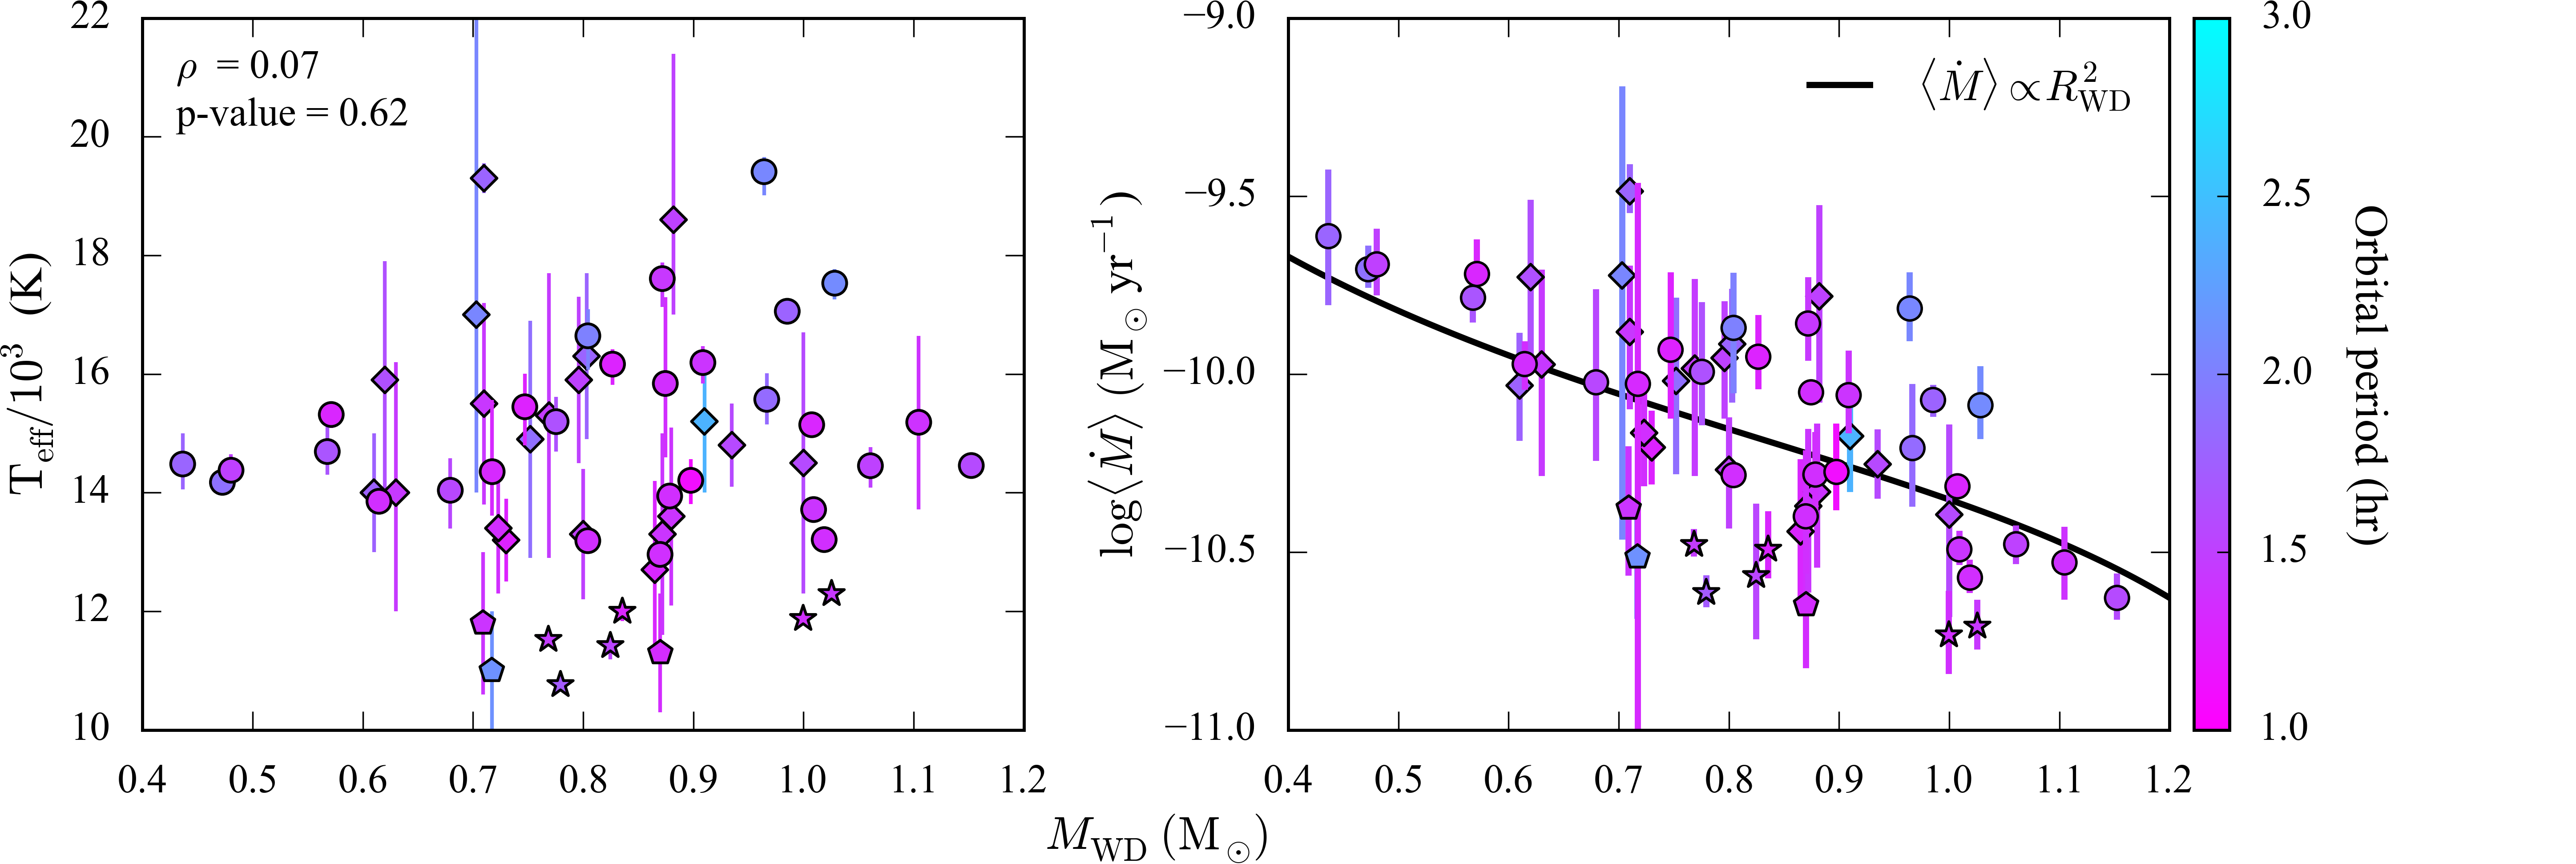
\includegraphics[width=\textwidth]{figures/modelling/pala_2022_fig13.png}
%     \caption{Reproduced from \citet{Pala2021}, Figure~13. The subset of modelled systems, with $P < 3{\rm hr}$ are shown. {\bf Circles} and {\bf stars} are pre- and post-period bounce systems derived by \citet{Pala2021}, and {\bf diamonds} and {\bf pentagons} are pre- and post-period bounce systems taken from the literature. {\it Left}: The $T_{\rm eff}$ is plotted against $M_{\rm wd}$, and no correlation can be seen. {\it Right}: $\log \langle \dot M \rangle$ is plotted against $M_{\rm wd}$, though now the data are correlated along the white dwarf mass-radius relationship outlined by \citet{Pala2021}, $M_{\rm wd} \propto R_{\rm wd}^{2}$, shown by the {\bf black line}.}
%     \label{fig:modelling:pala2022 fig13}
% \end{figure}


\begin{table}
    \centering
    \caption{The $\dot M$ found using the white dwarf properties for each system with a $\dot M$ measurement from donor properties. Sources are keyed the same as Table~\ref{table:results:mdot modelling}}
    \label{table:results:Mdot from white dwarf parameters}
    \begin{tabular}{llccc}
        \hline
        \textbf{Name} & \textbf{Source} & \textbf{$M_{\rm wd}, M_\odot$} & \textbf{$T_{\rm eff}$, K} & \textbf{$\log (\dot M, M_\odot {\rm yr}^{-1})$} \\
        \hline \hline \\
        ASASSN-14hq      &  W22  & $0.67 \pm 0.01$ & $14800\pm   800$ & $ -9.93 \pm 0.02$ \\
        ASASSN-14kb      &  W22  & $0.74 \pm 0.02$ & $17700\pm  1000$ & $ -9.90 \pm 0.03$ \\
        ASASSN-15pb      &  W22  & $0.72 \pm 0.03$ & $19200\pm  1600$ & $ -9.85 \pm 0.04$ \\
        ASASSN-17fo      &  W22  & $0.85 \pm 0.01$ & $14800\pm   600$ & $-10.03 \pm 0.02$ \\
        AY For           &  W22  & $0.78 \pm 0.02$ & $18200\pm   500$ & $ -9.91 \pm 0.02$ \\
        CSS090102        &  W22  & $0.62 \pm 0.03$ & $14800\pm  1200$ & $ -9.90 \pm 0.04$ \\
        CSS090419        &  W22  & $0.59 \pm 0.08$ & $18200\pm  9000$ & $ -9.79 \pm 0.28$ \\
        CSS090622        &  W22  & $0.67 \pm 0.06$ & $ 9800\pm  1500$ & $-10.11 \pm 0.08$ \\
        MAS0014          &  W22  & $0.86 \pm 0.03$ & $17300\pm  1000$ & $ -9.97 \pm 0.03$ \\
        OGLE82           &  W22  & $0.84 \pm 0.02$ & $18000\pm  4400$ & $ -9.95 \pm 0.12$ \\
        SDSS J0748       &  W22  & $0.80 \pm 0.05$ & $28400\pm  3300$ & $ -9.73 \pm 0.06$ \\
        SDSS J1524       &  W22  & $0.99 \pm 0.01$ & $12500\pm   900$ & $-10.17 \pm 0.03$ \\
        ASASSN-16kr      &  W20  & $0.95 \pm 0.02$ & $11500\pm   300$ & $-10.19 \pm 0.01$ \\
        ASASSN-17jf      &  W20  & $0.70 \pm 0.03$ & $12020\pm   850$ & $-10.03 \pm 0.04$ \\
        SSSJ1502-3505    &  W20  & $0.76 \pm 0.02$ & $22800\pm  1500$ & $ -9.80 \pm 0.03$ \\
        CSS080623        &  M19  & $0.71 \pm 0.02$ & $15500\pm  1700$ & $ -9.94 \pm 0.05$ \\
        CSS110113        &  M19  & $1.00 \pm 0.05$ & $14500\pm  2200$ & $-10.11 \pm 0.07$ \\
        CTCV 1300-3052   &  M19  & $0.72 \pm 0.02$ & $11000\pm  1000$ & $-10.09 \pm 0.04$ \\
        DV UMa           &  M19  & $1.09 \pm 0.03$ & $17400\pm  1900$ & $-10.07 \pm 0.05$ \\
        GY Cnc           &  M19  & $0.88 \pm 0.02$ & $25900\pm  2300$ & $ -9.81 \pm 0.04$ \\
        IY UMa           &  M19  & $0.96 \pm 0.01$ & $18000\pm  1000$ & $-10.00 \pm 0.02$ \\
        OY Car           &  M19  & $0.88 \pm 0.02$ & $18600\pm  2800$ & $ -9.95 \pm 0.07$ \\
        SDSS J0901       &  M19  & $0.75 \pm 0.02$ & $14900\pm  2000$ & $ -9.98 \pm 0.06$ \\
        SDSS J1006       &  M19  & $0.82 \pm 0.11$ & $16500\pm  2000$ & $ -9.97 \pm 0.08$ \\
        SDSS J1152       &  M19  & $0.62 \pm 0.04$ & $15900\pm  2000$ & $ -9.87 \pm 0.06$ \\
        SDSS J1501       &  M19  & $0.72 \pm 0.02$ & $14900\pm  1000$ & $ -9.96 \pm 0.03$ \\
        SSS100615        &  M19  & $0.88 \pm 0.03$ & $13600\pm  1500$ & $-10.09 \pm 0.05$ \\
        SSS130413        &  M19  & $0.84 \pm 0.03$ & $24000\pm  3000$ & $ -9.82 \pm 0.06$ \\
        V713 Cep         &  M19  & $0.70 \pm 0.02$ & $17000\pm  6000$ & $ -9.89 \pm 0.19$ \\
        Z Cha            &  M19  & $0.80 \pm 0.01$ & $16300\pm  1400$ & $ -9.97 \pm 0.04$ \\
        SDSS J1057       &  M17a & $0.80 \pm 0.02$ & $13300\pm  1100$ & $-10.06 \pm 0.04$ \\
        ASASSN-14ag      &  M17b & $0.63 \pm 0.04$ & $14000\pm  2100$ & $ -9.93 \pm 0.07$ \\
        PHL 1445         &  M15  & $0.73 \pm 0.03$ & $13200\pm   700$ & $-10.02 \pm 0.03$ \\
        \hline
    \end{tabular}
\end{table}

\begin{table}
    \centering
    \caption{Table~\ref{table:results:Mdot from white dwarf parameters}, continued}
    \label{table:results:Mdot from white dwarf parameters cont}
    \begin{tabular}{llccc}
        \hline
        \textbf{Name} & \textbf{Source} & \textbf{$M_{\rm wd}, M_\odot$} & \textbf{$T_{\rm eff}$, K} & \textbf{$\log (\dot M, M_\odot {\rm yr}^{-1})$} \\
        \hline \hline \\
        CTCV J1300-3052  &  S11  & $0.74 \pm 0.01$ & $11100\pm   800$ & $-10.10 \pm 0.03$ \\
        CTCV J2354-4700  &  S11  & $0.94 \pm 0.03$ & $14800\pm   700$ & $-10.08 \pm 0.02$ \\
        SDSS J1152       &  S11  & $0.56 \pm 0.03$ & $12400\pm  1400$ & $ -9.93 \pm 0.06$ \\
        OU Vir           &  S11  & $0.70 \pm 0.01$ & $22300\pm  2100$ & $ -9.77 \pm 0.04$ \\
        % DV UMa           &  S11  & $1.10 \pm 0.02$ & $15500\pm  2400$ & $-10.13 \pm 0.07$ \\
        XZ Eri           &  S11  & $0.77 \pm 0.02$ & $15300\pm  1900$ & $ -9.98 \pm 0.06$ \\
        SDSS J1702       &  S11  & $0.91 \pm 0.03$ & $15200\pm  1200$ & $-10.05 \pm 0.04$ \\
        SDSS J1035       &  S11  & $0.84 \pm 0.01$ & $10000\pm  1100$ & $-10.20 \pm 0.05$ \\
        SDSS J1507       &  S11  & $0.89 \pm 0.01$ & $11300\pm  1000$ & $-10.17 \pm 0.04$ \\
        SDSS J0903       &  S11  & $0.87 \pm 0.01$ & $13300\pm  1700$ & $-10.09 \pm 0.06$ \\
        SDSS J1227       &  S11  & $0.80 \pm 0.02$ & $15900\pm  1400$ & $ -9.98 \pm 0.04$ \\
        SDSS J1433       &  S11  & $0.87 \pm 0.01$ & $12700\pm  1500$ & $-10.11 \pm 0.05$ \\
        SDSS J1502       &  S11  & $0.709\pm0.004$ & $11800\pm  1200$ & $-10.05 \pm 0.04$ \\
        % SDSS J1501       &  S11  & $0.77 \pm 0.03$ & $10800\pm  1500$ & $-10.13 \pm 0.06$ \\
        IP Peg           &  C10  & $1.16 \pm 0.02$ & $12500\pm  2500$ & $-10.24 \pm 0.09$ \\
        \hline
    \end{tabular}
\end{table}





\chapter{Discussion}
\label{chpt:discussion} % for referencing this chapter elsewhere, use \ref{chpt:label}
\lhead{\emph{Discussion}} % This is for the header on each page - perhaps a shortened title

The analysis of this section includes eclipse modelled data from several sources: the 15 systems contained in this thesis, the 15 CVs characterised by \citet{McAllister2019}, and the 14 CVs modelled by \citet{Savoury2011}. An additional 4 systems from \citet{mcallister2015,mcallister2017, mcallister2017b}; and \citet{copperwheat2010} were used, detailed in Table~\ref{appendix:table:supplementary systems}. A full catalogue of all these data is given in Appendix~\ref{appendix:eclipse modelled CV data tables}.
There is some overlap between the data of \citet{McAllister2019} and \citet{Savoury2011}, and where this is the case the more recent findings of \citet{McAllister2019} are preferred.




\section{Inferring mass loss rate from donor properties}
\label{sect:discussion:evolutionary modelling}

First, I compare the mass loss rates of the donor inferred from donor properties, with the mass loss rates inferred from the white dwarf properties. Figure~\ref{fig:discussion:compare Mdot from donor and WD} plots the $\dot M$ from each method, and two differences between the data are immediately obvious: the white dwarf properties consistently indicate a higher $\dot M$, and using the donor properties results in significantly larger uncertainties.

The white dwarf indicating a higher mass loss rate is expected, as recent dwarf novae (a.k.a periods of intense accretion onto the white dwarf) cause the surface to heat up, but after a dwarf nova has subsided the white dwarf will take hundreds to tens of thousands of years to adjust to the lower accretion rate.
Several of the CVs in this sample were identified for eclipse modelling follow-up \textit{explicitly} based on observations of recent outbursts, so it is unsurprising that the white dwarf can indicate $\dot M$ an order of magnitude higher than the donor suggests. As the white dwarf is subject to inflation by these short-term variations, the donor-based method is considered more reliable for the long-term $\dot M$ baseline and hereafter when values of $\dot M$ are used, they are the values derived from the donor properties.
\begin{figure}
    \centering
    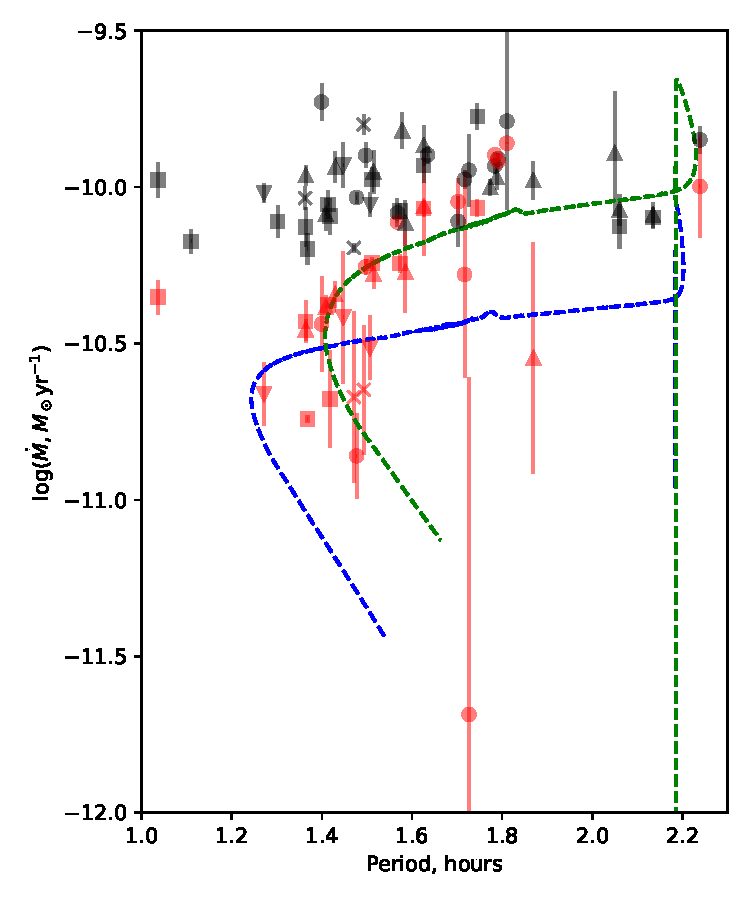
\includegraphics[width=\textwidth]{figures/results/Mdot/compare_mdot_from_donor_vs_wd_vs_period.pdf}
    \caption{Comparing the mass loss rates inferred from the donor properties ({\bf red crosses}) with those inferred from the white dwarf properties ({\bf blue crosses}).}
    \label{fig:discussion:compare Mdot from donor and WD}
\end{figure}


\subsection{Mass loss rate correlations}

Recall from the discussion in \S\ref{sect:introduction:magnetic braking} that, if the missing AML from CV models is rooted in residual magnetic braking, {\it and these prescriptions for magnetism are accurate}, we would expect to see a correlation between $M_{\rm donor}$ and $\dot M$. No such correlation is expected with $M_{\rm wd}$.
This is because both prescriptions are dependent on the Rossby number, a function of the rotational period, which itself is a function of donor mass for short period CVs.
If, however, the eCAML model is correct and the source of the missing AML is the white dwarf's ejecta carrying momentum with it from the system (refer to \S\ref{sect:introduction:CAML}), we would expect a correlation between $M_{\rm wd}$ and $\dot M$.
Of course, the two sources of extra AML are not mutually exclusive, and may co-exist.

To probe for these correlations the $\chi^2$ test is insufficient, since both axes have significant uncertainty. The orthogonal distance between the line and data is again minimised, similar to the previous section.

Figure~\ref{fig:discussion:donor mass vs Mdot fit} shows the best fit line for $\dot M(M_{\rm donor})$, and Figure~\ref{fig:discussion:white dwarf mass vs Mdot fit} is the fit for $\dot M(M_{\rm wd})$.

The correlation between $M_{\rm wd}$ and $\dot M$, is reasonably confident -- the best-fit gradient is $4.5\sigma$ from the null-hypothesis of 0.

However, no correlation is found between $\dot M$ and $M_{\rm donor}$, and Figure~\ref{fig:discussion:donor mass vs Mdot fit} clearly shows an incredibly wide range of gradients to be consistent with the data. If errors are ignored, the data have a Pearson's rank correlation coefficient of

Based on these results, it is unlikely that residual magnetic braking is responsible for the excess AML in CVs, but still possible that the drag imposed by nova material is the cause.
However, there are a few factors to consider when deciding how convincing these findings are.
The sample size is still small, only 25 systems, and the uncertainty in $\dot M$ are large. In addition, there may be a problem with systematic error -- it may that this sample is biased towards CVs with more excess AML, as these would be more inflated and thus less likely to be smaller than the Brown relation suggests for a zero-$\dot M$ star.
A significant source of unreliability is likely to be the mass-radius relationship used to calibrate the donor models. A more robust understanding of the low-mass main sequence mass-radius relation is crucial to a more confident re-analysis of these results.

\begin{figure}
    \centering
    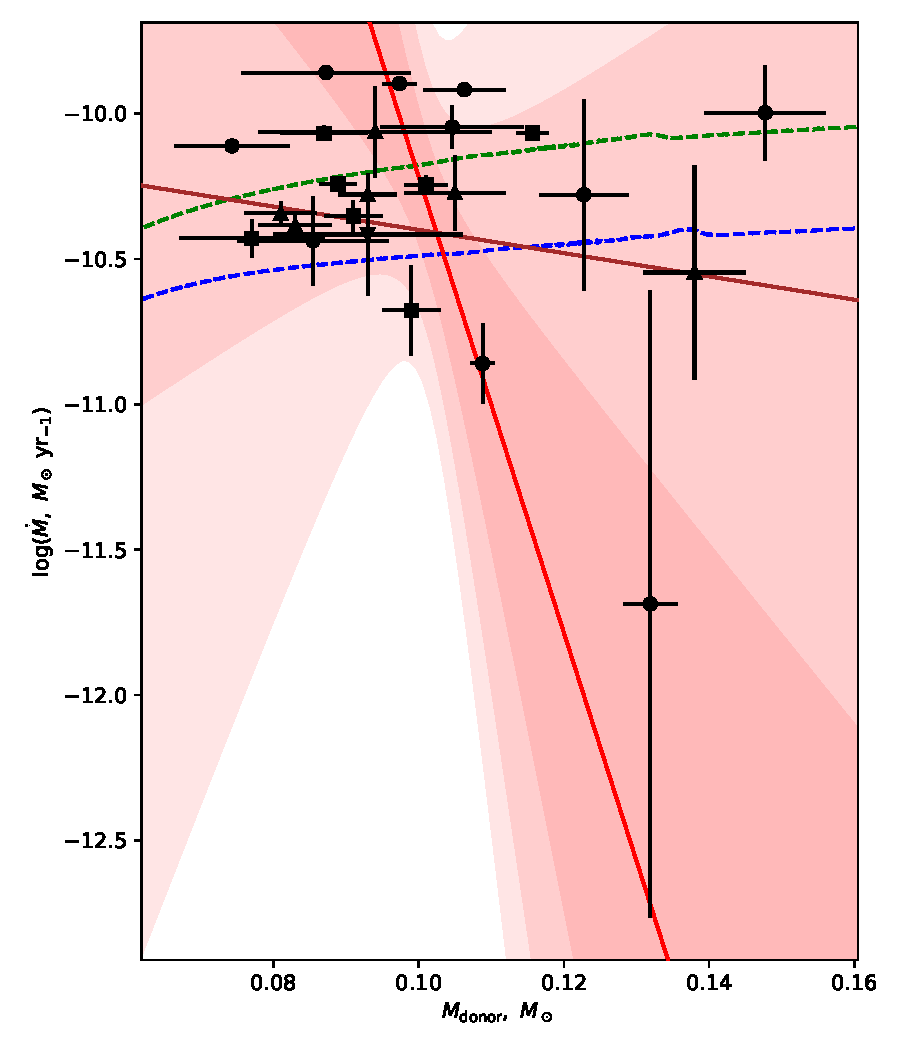
\includegraphics[width=\textwidth]{figures/results/Mdot/Mr_Mdot.pdf}
    \caption{Showing the correlation between the donor mass and mass loss rate. The {\bf black crosses with error bars} show the observations, and the {\bf red line} shows the best fit to the data, with the {\bf shaded red region} showing the coverage of the uncertainty in the line parameters. The darkest region is $1\sigma$, the middle region is $2\sigma$, and the lightest region shows $3\sigma$, and the {\rm brown line} is the initial guess for fitting. The {\bf dashed blue line} shows the value predicted by the `standard' MESA CV model, and the {\bf dashed green line} is the `optimal' MESA CV track. The best fit line has the form $\log (\dot M,\ M_\odot\ {\rm yr}^{-1}) = (-79\pm48) (M_{\rm donor}, M_\odot) - (2.3\pm4.9)$. }
    \label{fig:discussion:donor mass vs Mdot fit}
\end{figure}
% \begin{figure}
%     \centering
%     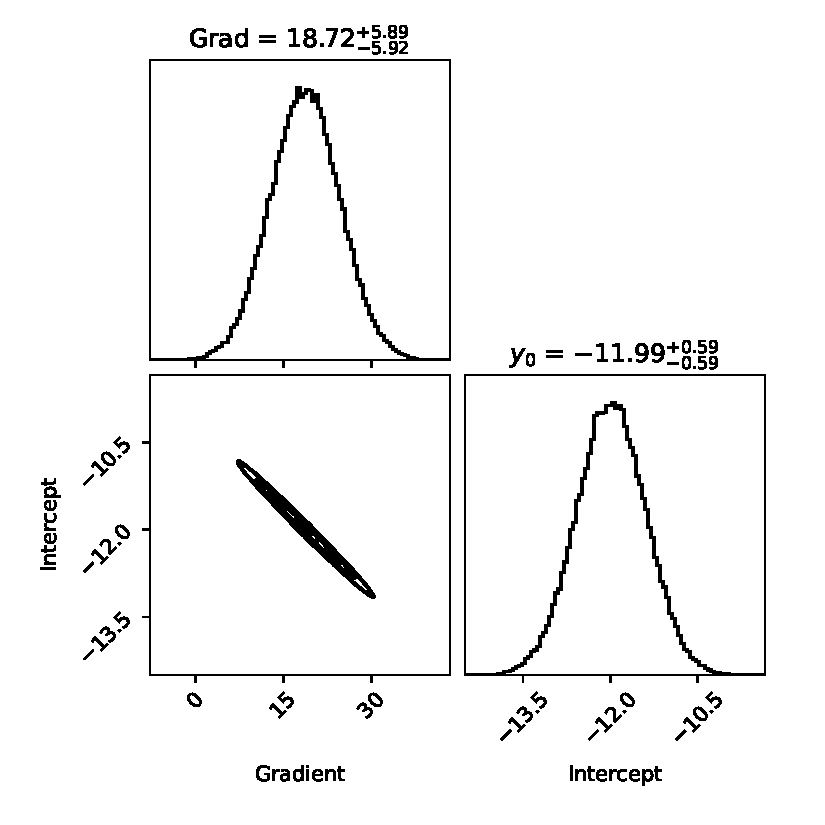
\includegraphics[width=\textwidth]{figures/results/Mdot/Mr_Mdot_corner.pdf}
%     \caption{Showing the posterior distributions of the gradient and intercept of the best fit line in Figure~\ref{fig:discussion:donor mass vs Mdot fit}.}
%     \label{fig:discussion:donor mass vs Mdot corner}
% \end{figure}
\begin{figure}
    \centering
    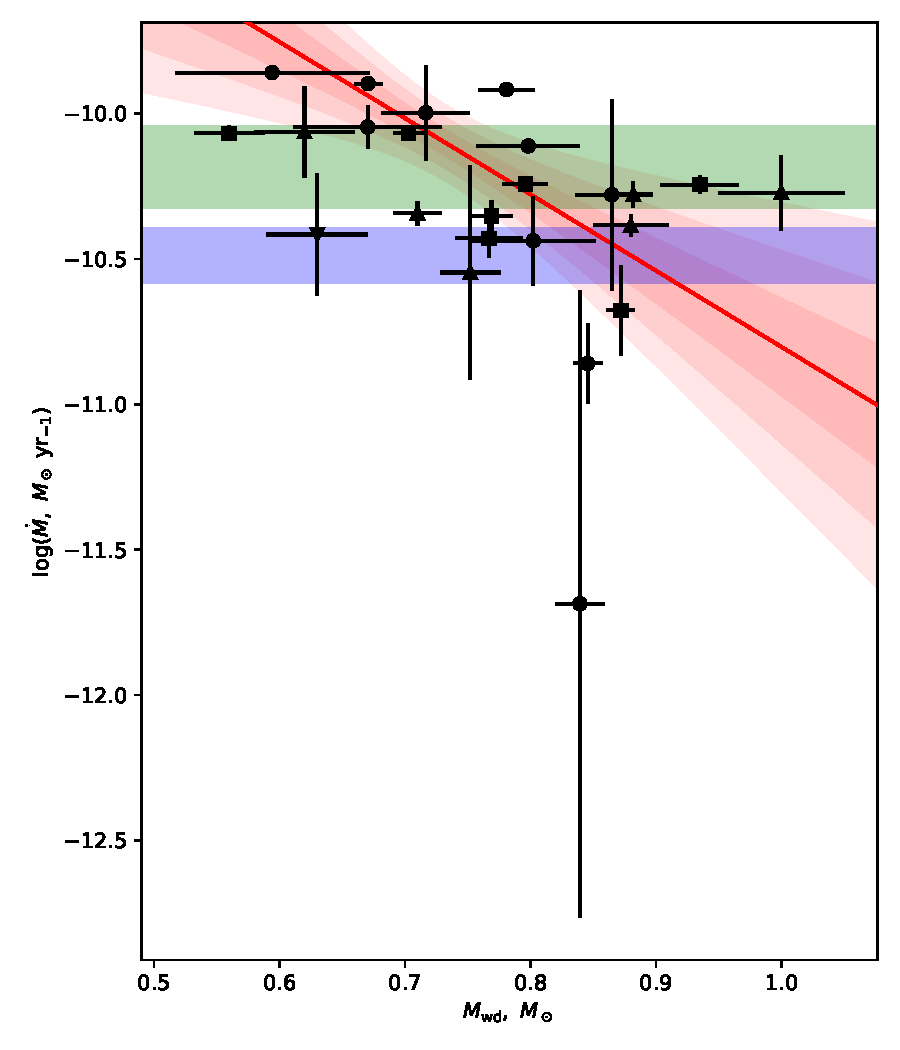
\includegraphics[width=\textwidth]{figures/results/Mdot/Mwd_Mdot.pdf}
    \caption{Showing the correlation between the white dwarf mass and mass loss rate. Symbols are similar to Figure~\ref{fig:discussion:donor mass vs Mdot fit}, though here the range of values predicted by the `standard' and `optimal' MESA CV models are shown as the {\bf blue shaded region} and {\bf green shaded region}, respectively. The best fit line has the form $\log ( \dot M,\ M_\odot\ {\rm yr}^{-1}) = (-2.62 \pm 0.60) (M_{\rm wd}, M_\odot) - (8.18 \pm 0.44)$}
    \label{fig:discussion:white dwarf mass vs Mdot fit}
\end{figure}
% \begin{figure}
%     \centering
%     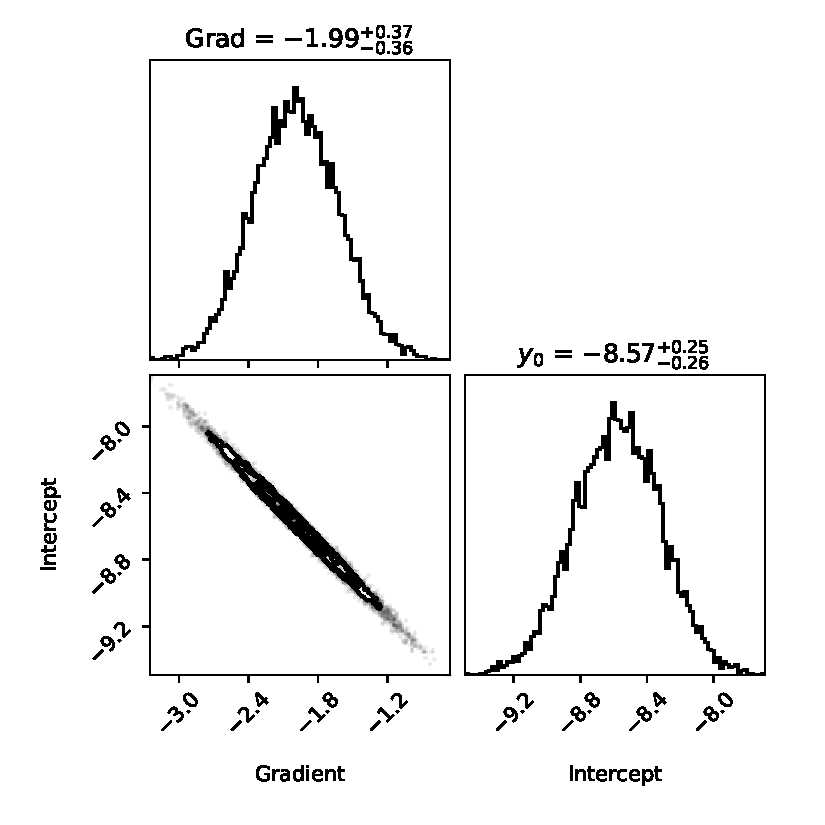
\includegraphics[width=\textwidth]{figures/results/Mdot/Mwd_Mdot_corner.pdf}
%     \caption{Showing the posterior distributions of the gradient and intercept of the best fit line in Figure~\ref{fig:discussion:white dwarf mass vs Mdot fit}.}
%     \label{fig:discussion:white dwarf mass vs Mdot corner}
% \end{figure}


\subsection{Measured excess angular momentum loss}

It is possible to more directly probe the AML of the CVs -- Equation~\ref{eqn:modelling:Jdot from Mdot} shows how the AML can be calculated from $M_{\rm wd},\ M_{\rm donor},\ \dot M$, and $a$.
Figures~\ref{fig:discussion:donor mass vs Jdot fit}~and~\ref{fig:discussion:white dwarf mass vs Jdot fit} show the best-fit to the $\dot J$ \textit{excess}, which has had the $\dot J_{\rm GR}$ predicted by MESA at the appropriate donor mass ($\dot J_{\rm MESA}$) subtracted.
Here, the white dwarf mass shows a reasonably confident correlation with the observed $\dot J$ excess, but with large scatter about the best-fit relationship. Similarly to the case of $\dot M$, fitting was unable to find a correlation between $M_{\rm donor}$ and $\dot J$ excess.

\begin{figure}
    \centering
    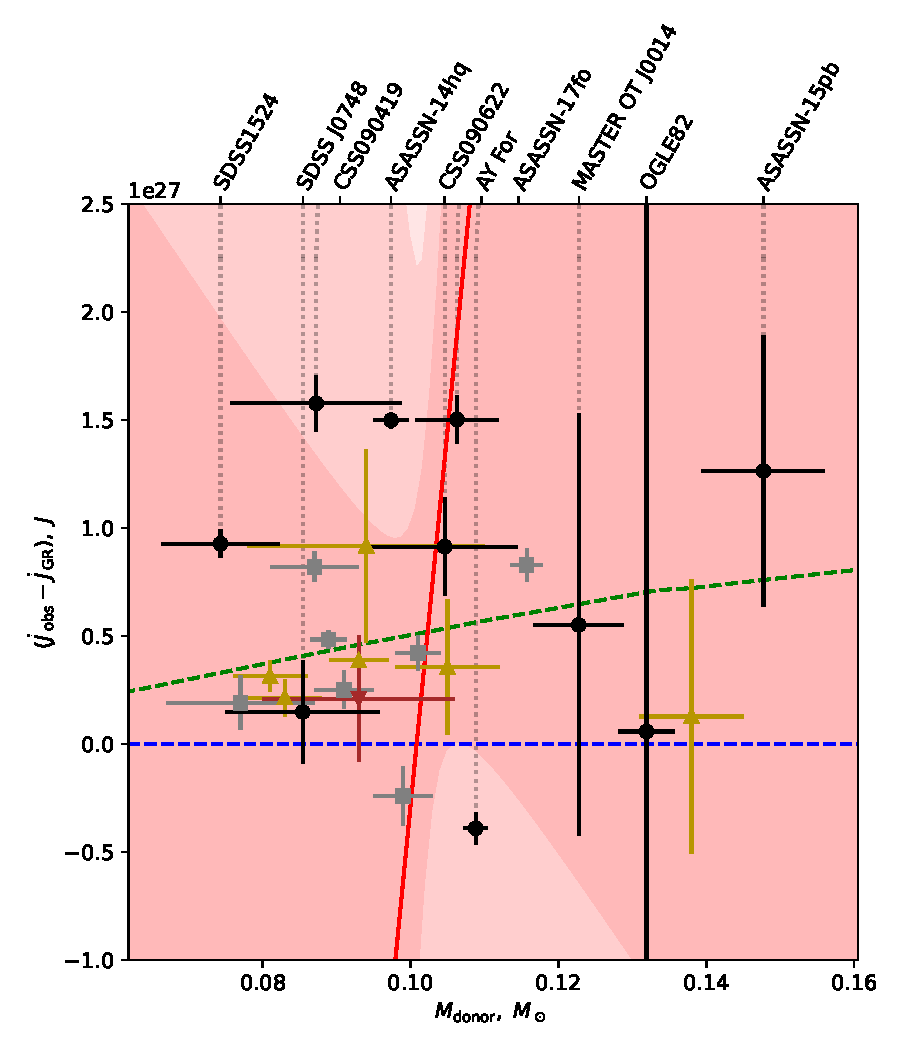
\includegraphics[width=\textwidth]{figures/results/Mdot/Mr_Jdot_ex.pdf}
    \caption{Showing the correlation between the donor mass and angular momentum loss rate, $\dot J$. Symbols are similar to Figure~\ref{fig:discussion:donor mass vs Mdot fit}, though here the {\bf dashed blue line} shows perfect agreement between observations and gravitational angular momentum loss. Note that the datum with vertical errors spanning the full height of the plot extend by approximately an order of magnitude in each direction, but are truncated for clarity. The line of best fit has the form $(\dot J_{\rm obs} - \dot J_{\rm MESA}), J = (5\pm10) \times 10^{29}(M_{\rm donor}, M_\odot) - (5\pm10)\times10^{28}$}
    \label{fig:discussion:donor mass vs Jdot fit}
\end{figure}
% \begin{figure}
%     \centering
%     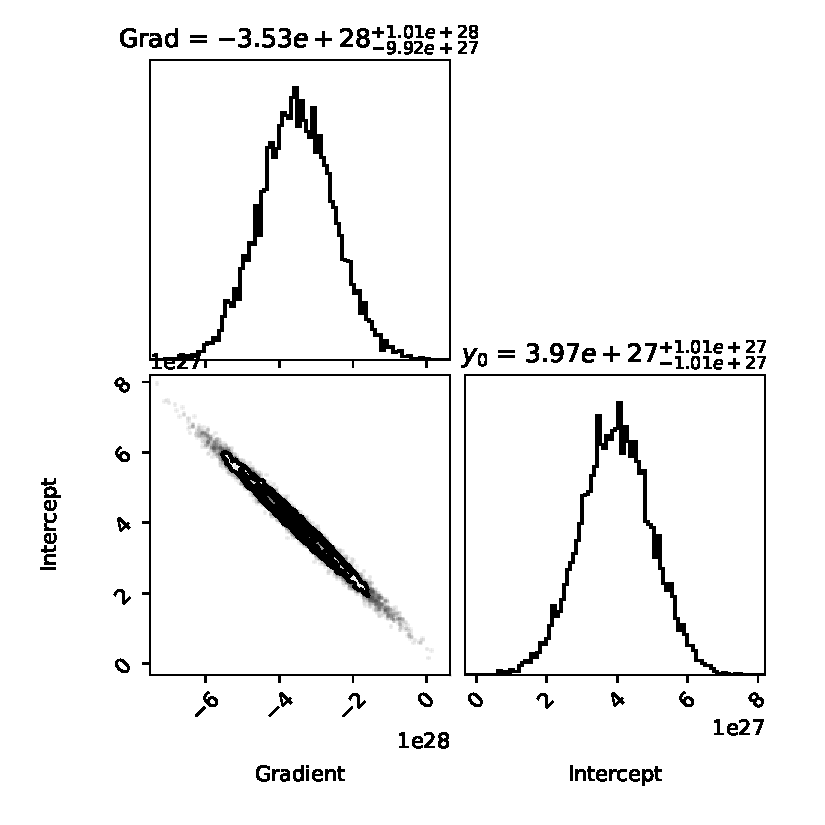
\includegraphics[width=\textwidth]{figures/results/Mdot/Mr_Jdot_ex_corner.pdf}
%     \caption{Showing the posterior distributions of the gradient and intercept of the best fit line in Figure~\ref{fig:discussion:donor mass vs Jdot fit}.}
%     \label{fig:discussion:donor mass vs Jdot corner}
% \end{figure}

\begin{figure}
    \centering
    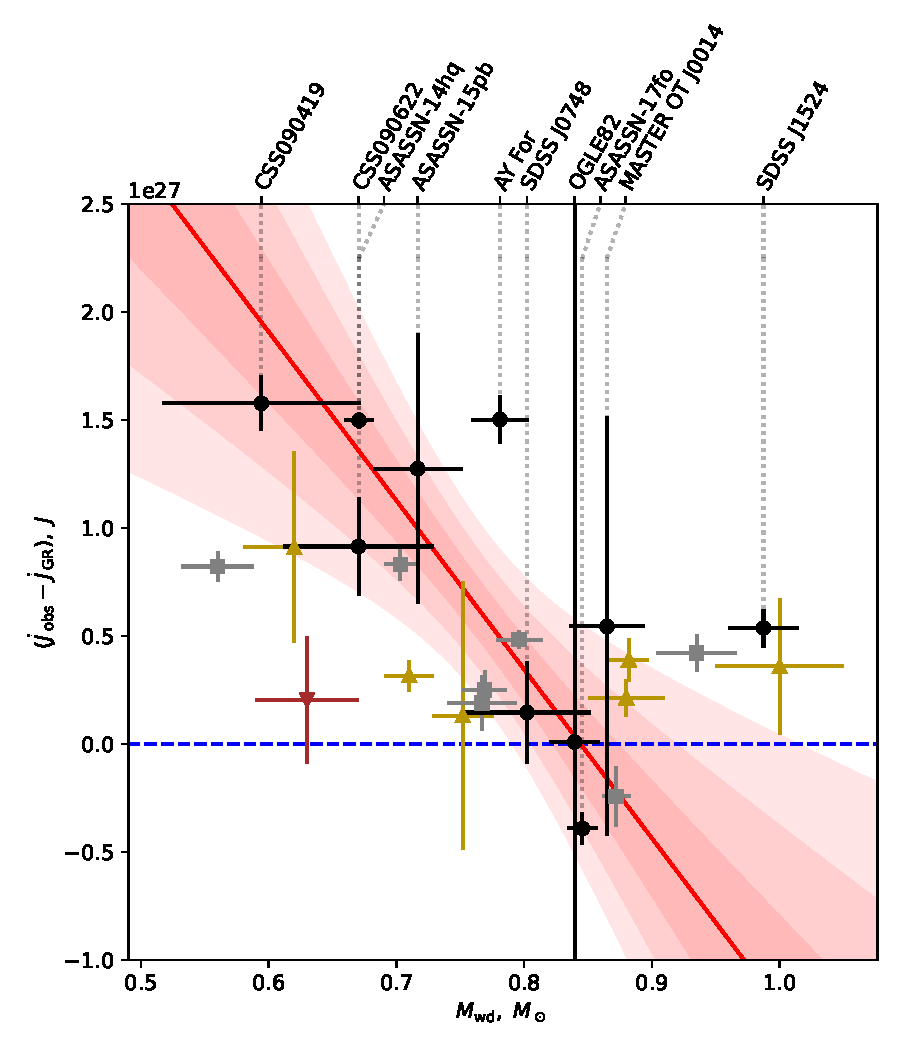
\includegraphics[width=\textwidth]{figures/results/Mdot/Mwd_Jdot_ex.pdf}
    \caption{Showing the correlation between the white dwarf mass and angular momentum loss rate, $\dot J$. Symbols are similar to Figure~\ref{fig:discussion:white dwarf mass vs Jdot fit}, and the best fit line has the form $(\dot J_{\rm obs} - \dot J_{\rm MESA}), J = -5.7\pm1.3) \times 10^{27}(M_{\rm wd}, M_\odot) - (4.6\pm0.96)\times10^{26}$}
    \label{fig:discussion:white dwarf mass vs Jdot fit}
\end{figure}
% \begin{figure}
%     \centering
%     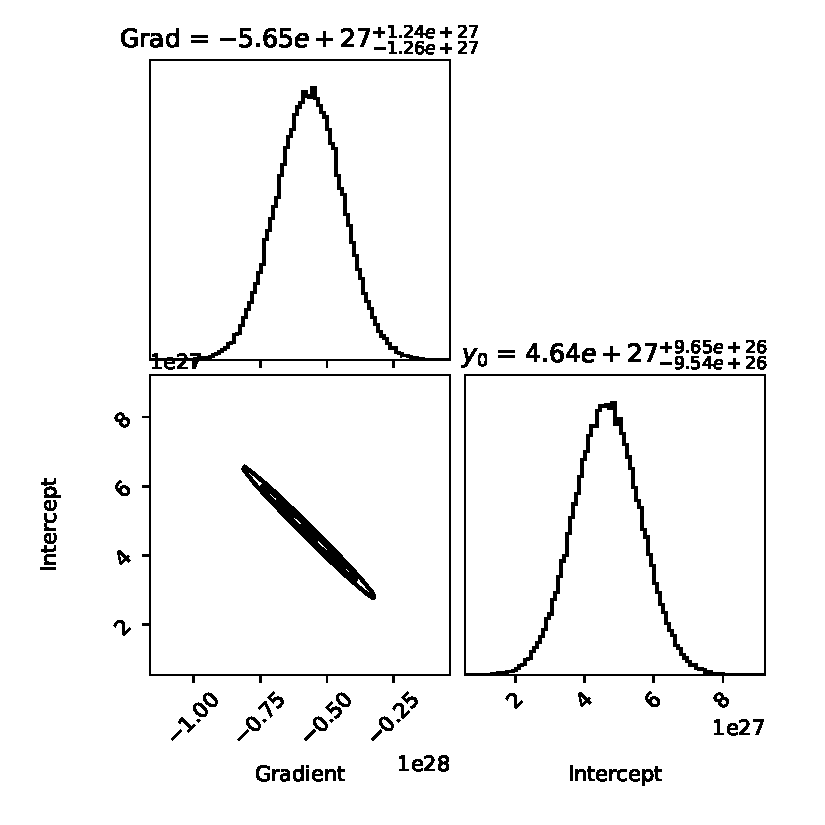
\includegraphics[width=\textwidth]{figures/results/Mdot/Mwd_Jdot_ex_corner.pdf}
%     \caption{Showing the posterior distributions of the gradient and intercept of the best fit line in Figure~\ref{fig:discussion:white dwarf mass vs Jdot fit}.}
%     \label{fig:discussion:white dwarf mass vs Jdot corner}
% \end{figure}


Three possibilities for the form of excess AML were suggested in \S\ref{sect:discussion AML}: the excess AML also declines in strength but more slowly than gravitational losses; excess AML is roughly constant across the range of $M_{\rm donor}$ or $M_{\rm donor}$; or excess AML increases in strength towards lower $M_{\rm donor}$ or $M_{\rm wd}$.
We can now see that the excess AML appears to increase in strength towards lower $M_{\rm wd}$.

% Based on the analysis above, it appears that eCAML is the better model for the excess AML of a short period CV, with there being consistent signs of increasing excess AML towards both lower donor masses, and lower white dwarf masses.
% We can now discriminate between these with the quantitative analysis given here, and see that the degree of excess AML is most likely to be a negative correlation with $M_{\rm wd}$, in line with the CAML model of CVs.


Recall from \S\ref{sect:introduction:CAML} that under eCAML, the efficiency parameter $\nu$, is given by $C/M_{\rm wd}$, and typical values of $C$ are roughly chosen to be $0.3 - 0.4$, to reproduce the observed CV population distribution.
\begin{equation}
    \label{eqn:ecaml general}
    \frac{\dot J_{CAML}}{J} = \nu \frac{\dot M_{\rm donor}}{M_{\rm donor}}
\end{equation}
Assuming that eCAML is the sole source of excess AML, we can now measure a value of $\nu$. To do this, I use a slightly modified version of Equation~\ref{eqn:ecaml general}, which accounts for the choice of the form of $\nu$;
\begin{equation}
    \frac{\dot J_{CAML}}{J} = C \frac{\dot M_{\rm donor}}{M_{\rm donor} M_{\rm wd}}
\end{equation}
$C$ can then be fit to data, again minimising the orthogonal distance to the data, though this fit is limited to the subset of the observations for which $\dot M$ could be determined.
Doing so finds a best-fit $C = 0.32 \pm0.05$ with impressively good agreement between the model and data, shown in Figure~\ref{fig:discussion:calibrating ecaml relationship}. This value of $C$ is also remarkably close to that estimated by \citet{Schreiber2016}. \todo{This is the wrong one! I need the one with no y-intercept.}
\begin{figure}
    \centering
    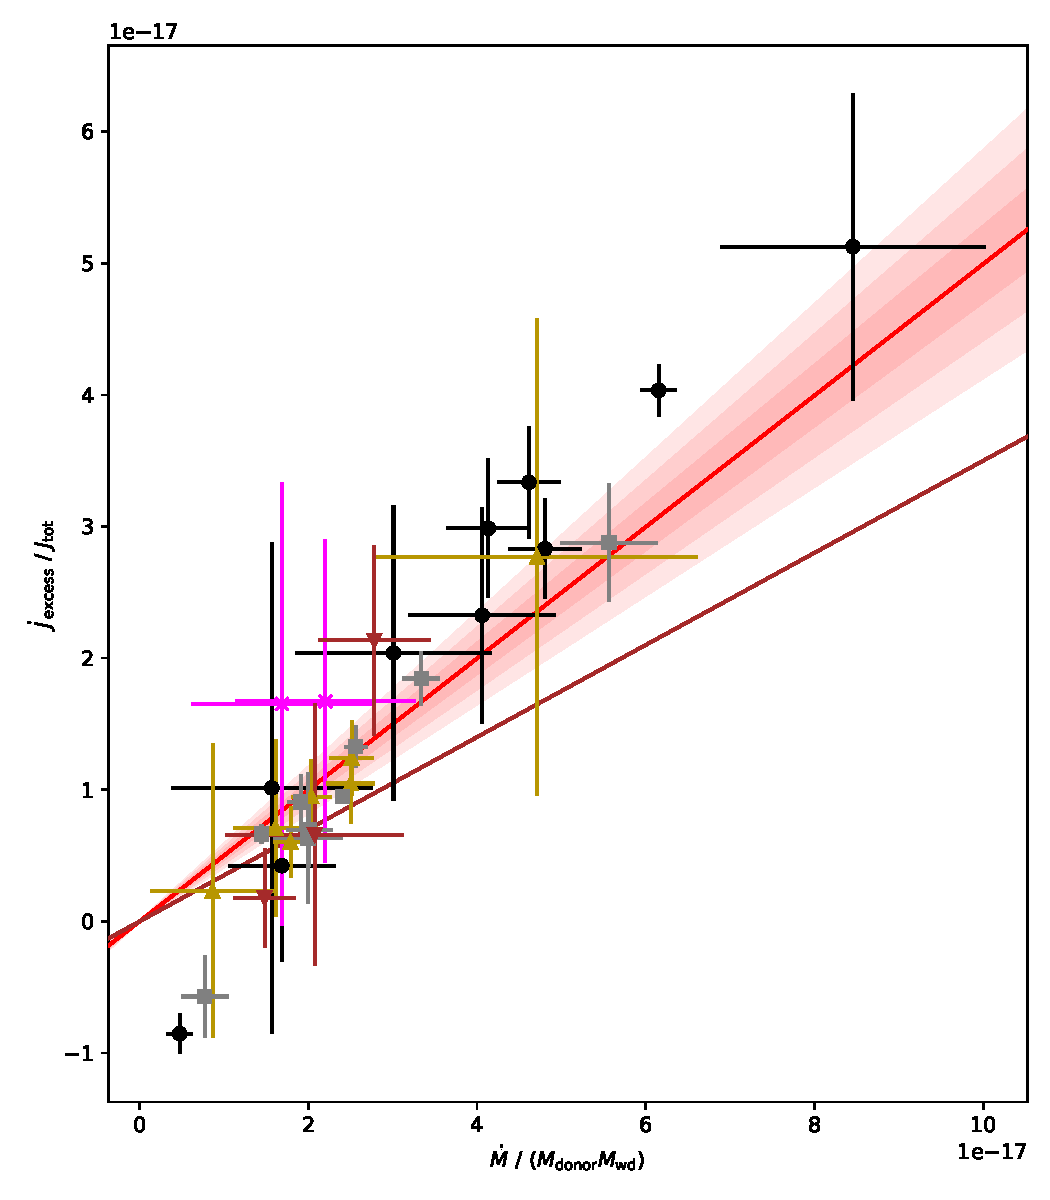
\includegraphics[width=\textwidth]{figures/results/Mdot/eCAML_nu_no_intercept_fit.pdf}
    \caption{DO THIS CAPTION}
    \label{fig:discussion:calibrating ecaml relationship}
\end{figure}

As a final test of eCAML, the stability plot given in Figure~\ref{fig:introduction:Schreiber 2016 figure 2} can be augmented to include the new CVs of this work, and the best-fit value of $\nu$.\todo{Fix the label!}
This is shown in Figure~\ref{fig:discussion:calibrated eCAML}, from which we can see that no low $M_{\rm donor}$ CVs exist outside the stability region demanded by the newly calibrated eCAML.
\begin{figure}
    \centering
    \includegraphics[width=\textwidth]{figures/results/Mdot/ecaml_nointercept.pdf}
    \caption{Showing the distribution of eclipse modelled, low $M_{\rm donor}$ CVs compared to the region of stability demanded by eCAML. The {\bf shaded grey regions} are forbidden, either because the white dwarf exceeds the Chandrasekhar limit (lower region), or because mass transfer becomes dynamically unstable (upper region). The {\bf dashed line} shows the mass ratio that a CV would have with $M_{\rm wd} = 0.81 M_\odot$. Data symbology is similar to Figure~\ref{fig:discussion:donor model with eclipsers plotted}}
    \label{fig:discussion:calibrated eCAML}
\end{figure}
These findings underline the success of eCAML in describing CV evolution, but must still be treated with caution. It cannot be ignored that whilst this form of $\nu$ is loosely physically motivated, a less empirical model is highly desirable.
Further, the data clearly suggest that $\frac{\dot J_{CAML}}{J} \neq 0$ at $\dot M = 0$, in direct contradiction with the original formulation. \todo{Talk to Stu about this when he's back. I reckon some algebra is needed to re-derive the stability criterion to allow for this... But it's not physical! How could CAML inhibit AML???}

Further work is needed to grow the population of eclipse modelled low-$M_{\rm donor}$ CVs and improve these statistics, and continued eclipse modelling targeting short period CVs will be valuable to determining the probable source of excess AML.
Specific effort should be targeted towards confident characterisation of CVs at higher $M_{\rm donor}$ of $\sim0.15$, where existing data have large error bars. The clustering of confident data at lower masses leaves the current sample prone to poor extrapolation beyond $\sim 0.11 M_\odot$.
However, lending credence to these results is the consistency with findings of \citet{Pala2021}, who used the white dwarf properties to arrive at a similar conclusion.

\todo{Augment MESA to include my new AML prescription, and run it?}

\chapter{Conclusion and future work}
\label{chpt:conclusion} % for referencing this chapter elsewhere, use \ref{chpt:label}
\lhead{\emph{Conclusion and future work}} % This is for the header on each page - perhaps a shortened title

who the hell knows. What more can I say?

\subsection{Conclusion}

The component masses and radii, separations, white dwarf temperatures and surface gravities of 15 new short-period CVs are contributed to the population of well-characterised CV observations, including two with extremely low-mass donor stars, and one which appears to be in the process of evolving through the period minimum.
Some issues were encountered during the modelling of a handful of systems, which are recommended for UV spectroscopic followup studies to probe them in more detail: $T_{\rm eff}$ of the white dwarf in SSSJ0522-3505 appears to be $\sim$10000K higher than is typical for a CV, and the white dwarfs of CSS090419 and CSS090622 appear to \textit{brighten} in the $i'$ band, contrary to models.
% The derived temperature is quite uncertain, but the origin of the discrepancy cannot confidently be determined, though possible causes are given.
% All three of the newly modelled systems lie within $1\sigma$ of the ``optimal'' model mass-radius evolutionary tracks from \citet{knigge11}.

The ``optimal'' donor tracks add an extra source of AML that takes the form of $\sim 1.5$ times the GWB. By examining the period excess between the initial set of observed CV donor radii and models, this can be demonstrated to probably be inconsistent with the missing AML seen in observations.
Rather than tracking the GWB as the CV evolves to lower masses, excess AML appears to grow in strength relative to gravitational losses as the donor shrinks. These preliminary findings did {\it not} find evidence for a relationship between excess AML strength, and $M_{\rm wd}$.
These preliminary findings were corroborated by detailed evolutionary modelling; MESA was used to infer the $\dot M$ rate of a CV based on the mass loss-induced inflation measured using eclipse modelling, and a



\end{onehalfspace}
% \end{doublespace}

\begin{singlespace}

%%%% BIBLIOGRAPHY BIBLIOGRAPHY BIBLIOGRAPHY BIBLIOGRAPHY%%%%%
\bibliographystyle{mn2e} %requires mn2e.bst file in same directory

% YOUR PATH %
\bibliography{thesis}

\end{singlespace}

%%%%%%%%%%%%%%%% APPENDIX APPENDIX APPENDIX APPENDIX %%%%%%%%%%%%%55
\onehalfspacing
\appendix
%Appenndix for line measurements in IRTF + other spectra

%\label{app:line_measure}
\chapter{Appendix}
\lhead{\emph{Appendix}}
\label{app:my_appendix}

%%%%%%%%%%%%%%%%% APPENDICES %%%%%%%%%%%%%%%%%%%%%

\onecolumn
\section{Phase-folded eclipse models}
\label{appendix:lightcurves}

Here, the eclipse modelling  results for the 15 systems analysed in this thesis are presented. Note that for some systems, data were binned together where appropriate to reduce the complexity of the parameter space that must be explored. Which data were binned together is detailed in the observation logs contained in Appendix~\ref{sect:observing:observation catalogue}\todo{I think the tau-gp has been corrupted by the move from log to linear space. These plots have just the tau's unlogged, but they seem off. Fix this! Probably just a case of git checkout old branch.}

\begin{figure}
    \centering
    \includegraphics[width=\textwidth]{figures/results/three_cvs_with_weird_colours/ASASSN-17jf/ASASSN-17jf_1.pdf}
    \caption{ASASSN-17jf lightcurve models. {\it Top}:~{\bf grey points} are the observed flux, and note that the photometric system is the SDSS as per \S\ref{sect:observations:flux calibrating the lightcurve}; {\bf black line} is the observed flux, with the mean Gaussian process sample subtracted; the {\bf dark blue line} is the mean lightcurve model, and the {\bf blue band} is the standard deviation on this in the MCMC chain. The components of the model are also shown: the {\bf light blue line} is the white dwarf flux, {\bf green line} is the bright spot, {\bf orange line} is the disc, and the {\bf red line} is the donor. {\it Bottom}:~The residuals between the data and model are plotted as the {\bf black line}, with grey error bars. The Gaussian process 1-sigma region is shown as a {\bf red band}.}
    \label{fig:ASASSN-17jf all lightcurves}
\end{figure}
\begin{figure}
    \centering
    \includegraphics[width=\textwidth]{figures/results/three_cvs_with_weird_colours/ASASSN-17jf/ASASSN-17jf_2.pdf}
    \caption{ASASSN-17jf lightcurve models (cont.)}
    \label{fig:ASASSN-17jf all lightcurves cont 1}
\end{figure}
\begin{figure}
    \centering
    \includegraphics[width=\textwidth]{figures/results/three_cvs_with_weird_colours/ASASSN-17jf/ASASSN-17jf_3.pdf}
    \caption{ASASSN-17jf lightcurve models (cont.)}
    \label{fig:ASASSN-17jf all lightcurves cont 2}
\end{figure}



\begin{figure}
    \centering
    \includegraphics[width=\textwidth]{figures/results/three_cvs_with_weird_colours/ASASSN-16kr/ASASSN-16kr_1.pdf}
    \caption{ASASSN-16kr lightcurve models. Symbols are the same as Figure~\ref{fig:ASASSN-17jf all lightcurves}}
    \label{fig:ASASSN-16kr all lightcurves}
\end{figure}
\begin{figure}
    \centering
    \includegraphics[width=\textwidth]{figures/results/three_cvs_with_weird_colours/ASASSN-16kr/ASASSN-16kr_2.pdf}
    \caption{ASASSN-16kr lightcurve models (cont.)}
    \label{fig:ASASSN-16kr all lightcurves cont 1}
\end{figure}
\begin{figure}
    \centering
    \includegraphics[width=\textwidth]{figures/results/three_cvs_with_weird_colours/ASASSN-16kr/ASASSN-16kr_3.pdf}
    \caption{ASASSN-16kr lightcurve models (cont.)}
    \label{fig:ASASSN-16kr all lightcurves cont 2}
\end{figure}
\begin{figure}
    \centering
    \includegraphics[width=\textwidth]{figures/results/three_cvs_with_weird_colours/ASASSN-16kr/ASASSN-16kr_4.pdf}
    \caption{ASASSN-16kr lightcurve models (cont.)}
    \label{fig:ASASSN-16kr all lightcurves cont 3}
\end{figure}
\begin{figure}
    \centering
    \includegraphics[width=\textwidth]{figures/results/three_cvs_with_weird_colours/ASASSN-16kr/ASASSN-16kr_5.pdf}
    \caption{ASASSN-16kr lightcurve models (cont.)}
    \label{fig:ASASSN-16kr all lightcurves cont 4}
\end{figure}
\begin{figure}
    \centering
    \includegraphics[width=\textwidth]{figures/results/three_cvs_with_weird_colours/ASASSN-16kr/ASASSN-16kr_6.pdf}
    \caption{ASASSN-16kr lightcurve models (cont.)}
    \label{fig:ASASSN-16kr all lightcurves cont 5}
\end{figure}
\begin{figure}
    \centering
    \includegraphics[width=\textwidth]{figures/results/three_cvs_with_weird_colours/ASASSN-16kr/ASASSN-16kr_7.pdf}
    \caption{ASASSN-16kr lightcurve models (cont.)}
    \label{fig:ASASSN-16kr all lightcurves cont 6}
\end{figure}
\clearpage


\begin{figure}
    \centering
    \includegraphics[width=\textwidth]{figures/results/three_cvs_with_weird_colours/SSS111126/SSS111126_1.pdf}
    \caption{SSSJ0522-3505 lightcurve models. Symbols are the same as Figure~\ref{fig:ASASSN-17jf all lightcurves}}
    \label{fig:SSSJ0522-3505 all lightcurves}
\end{figure}
\begin{figure}
    \centering
    \includegraphics[width=\textwidth]{figures/results/three_cvs_with_weird_colours/SSS111126/SSS111126_2.pdf}
    \caption{SSSJ0522-3505 lightcurve models (cont.)}
    \label{fig:SSSJ0522-3505 all lightcurves cont 1}
\end{figure}
\begin{figure}
    \centering
    \includegraphics[width=\textwidth]{figures/results/three_cvs_with_weird_colours/SSS111126/SSS111126_3.pdf}
    \caption{SSSJ0522-3505 lightcurve models (cont.)}
    \label{fig:SSSJ0522-3505 all lightcurves cont 2}
\end{figure}
\clearpage



\begin{figure}
    \centering
    \includegraphics[width=\textwidth]{figures/results/ASASSN-14hq/ASASSN-14hq_1.pdf}
    \caption{ASASSN-14hq lightcurve models. Symbols are the same as Figure~\ref{fig:ASASSN-17jf all lightcurves}}
    \label{fig:ASASSN-14hq all lightcurves}
\end{figure}
\begin{figure}
    \centering
    \includegraphics[width=\textwidth]{figures/results/ASASSN-14hq/ASASSN-14hq_2.pdf}
    \caption{ASASSN-14hq lightcurve models (cont.)}
    \label{fig:ASASSN-14hq all lightcurves cont}
\end{figure}
\begin{figure}
    \centering
    \includegraphics[width=\textwidth]{figures/results/ASASSN-14hq/fluxplot.pdf}
    \caption{ASASSN-14hq observed white dwarf fluxes, compared to the best-fit model atmosphere.}
    \label{fig:ASASSN-14hq flux plot}
\end{figure}
\clearpage

\begin{figure}
    \centering
    \includegraphics[width=\textwidth]{figures/results/ASASSN-14kb/ASASSN-14kb_1.pdf}
    \caption{ASASSN-14kb lightcurve models. Symbols are the same as Figure~\ref{fig:ASASSN-17jf all lightcurves}}
    \label{fig:ASASSN-14kb all lightcurves}
\end{figure}
\begin{figure}
    \centering
    \includegraphics[width=\textwidth]{figures/results/ASASSN-14kb/fluxplot.pdf}
    \caption{ASASSN-14kb observed white dwarf fluxes, compared to the best-fit model atmosphere.}
    \label{fig:ASASSN-14kb flux plot}
\end{figure}
\clearpage


\begin{figure}
    \centering
    \includegraphics[width=\textwidth]{figures/results/ASASSN-15pb/ASASSN-15pb_1.pdf}
    \caption{ASASSN-15pb lightcurve models. Symbols are the same as Figure~\ref{fig:ASASSN-17jf all lightcurves}}
    \label{fig:ASASSN-15pb all lightcurves}
\end{figure}
\begin{figure}
    \centering
    \includegraphics[width=\textwidth]{figures/results/ASASSN-15pb/ASASSN-15pb_2.pdf}
    \caption{ASASSN-15pb lightcurve models (cont.)}
    \label{fig:ASASSN-15pb all lightcurves cont 1}
\end{figure}
\begin{figure}
    \centering
    \includegraphics[width=\textwidth]{figures/results/ASASSN-15pb/fluxplot.pdf}
    \caption{ASASSN-15pb observed white dwarf fluxes, compared to the best-fit model atmosphere.}
    \label{fig:ASASSN-15pb flux plot}
\end{figure}
\clearpage


\begin{figure}
    \centering
    \includegraphics[width=\textwidth]{figures/results/ASASSN-17fo/ASASSN-17fo_1.pdf}
    \caption{ASASSN-17fo lightcurve models. Symbols are the same as Figure~\ref{fig:ASASSN-17jf all lightcurves}}
    \label{fig:ASASSN-17fo all lightcurves}
\end{figure}
\begin{figure}
    \centering
    \includegraphics[width=\textwidth]{figures/results/ASASSN-17fo/ASASSN-17fo_2.pdf}
    \caption{ASASSN-17fo lightcurve models (cont.)}
    \label{fig:ASASSN-17fo all lightcurves cont 1}
\end{figure}
\begin{figure}
    \centering
    \includegraphics[width=\textwidth]{figures/results/ASASSN-17fo/ASASSN-17fo_3.pdf}
    \caption{ASASSN-17fo lightcurve models (cont.)}
    \label{fig:ASASSN-17fo all lightcurves cont 2}
\end{figure}
\begin{figure}
    \centering
    \includegraphics[width=\textwidth]{figures/results/ASASSN-17fo/fluxplot.pdf}
    \caption{ASASSN-17fo observed white dwarf fluxes, compared to the best-fit model atmosphere.}
    \label{fig:ASASSN-17fo flux plot}
\end{figure}
\clearpage


\begin{figure}
    \centering
    \includegraphics[width=\textwidth]{figures/results/AYFor/AYFor_1.pdf}
    \caption{AY For lightcurve models. Symbols are the same as Figure~\ref{fig:ASASSN-17jf all lightcurves}}
    \label{fig:AYFor all lightcurves}
\end{figure}
\begin{figure}
    \centering
    \includegraphics[width=\textwidth]{figures/results/AYFor/AYFor_2.pdf}
    \caption{AY For lightcurve models (cont.)}
    \label{fig:AYFor all lightcurves cont 1}
\end{figure}
\begin{figure}
    \centering
    \includegraphics[width=\textwidth]{figures/results/AYFor/AYFor_3.pdf}
    \caption{AY For lightcurve models (cont.)}
    \label{fig:AYFor all lightcurves cont 2}
\end{figure}
\begin{figure}
    \centering
    \includegraphics[width=\textwidth]{figures/results/AYFor/fluxplot.pdf}
    \caption{AY For observed white dwarf fluxes, compared to the best-fit model atmosphere.}
    \label{fig:AYFor flux plot}
\end{figure}
\clearpage


\begin{figure}
    \centering
    \includegraphics[width=\textwidth]{figures/results/CSS090102/CSS090102_1.pdf}
    \caption{CSS090102 lightcurve models. Symbols are the same as Figure~\ref{fig:ASASSN-17jf all lightcurves}}
    \label{fig:CSS090102 all lightcurves}
\end{figure}
\begin{figure}
    \centering
    \includegraphics[width=\textwidth]{figures/results/CSS090102/fluxplot.pdf}
    \caption{CSS090102 observed white dwarf fluxes, compared to the best-fit model atmosphere.}
    \label{fig:CSS090102 flux plot}
\end{figure}
\clearpage


\begin{figure}
    \centering
    \includegraphics[width=\textwidth]{figures/results/CSS090419/CSS090419_1.pdf}
    \caption{CSS090419 lightcurve models. Symbols are the same as Figure~\ref{fig:ASASSN-17jf all lightcurves}}
    \label{fig:CSS090419 all lightcurves}
\end{figure}
\begin{figure}
    \centering
    \includegraphics[width=\textwidth]{figures/results/CSS090419/CSS090419_2.pdf}
    \caption{CSS090419 lightcurve models (cont.)}
    \label{fig:CSS090419 all lightcurves cont 1}
\end{figure}
\begin{figure}
    \centering
    \includegraphics[width=\textwidth]{figures/results/CSS090419/fluxplot.pdf}
    \caption{CSS090419 observed white dwarf fluxes, compared to the best-fit model atmosphere.}
    \label{fig:CSS090419 flux plot}
\end{figure}
\clearpage


\begin{figure}
    \centering
    \includegraphics[width=\textwidth]{figures/results/CSS090622/CSS090622_1.pdf}
    \caption{CSS090622 lightcurve models. Symbols are the same as Figure~\ref{fig:ASASSN-17jf all lightcurves}}
    \label{fig:CSS090622 all lightcurves}
\end{figure}
\begin{figure}
    \centering
    \includegraphics[width=\textwidth]{figures/results/CSS090622/CSS090622_2.pdf}
    \caption{CSS090622 lightcurve models (cont.)}
    \label{fig:CSS090622 all lightcurves cont 1}
\end{figure}
\begin{figure}
    \centering
    \includegraphics[width=\textwidth]{figures/results/CSS090622/fluxplot.pdf}
    \caption{CSS090622 observed white dwarf fluxes, compared to the best-fit model atmosphere.}
    \label{fig:CSS090622 flux plot}
\end{figure}
\clearpage


\begin{figure}
    \centering
    \includegraphics[width=\textwidth]{figures/results/MASOT0014/MASOT0014_1.pdf}
    \caption{MAS0014 lightcurve models. Symbols are the same as Figure~\ref{fig:ASASSN-17jf all lightcurves}}
    \label{fig:MAS0014 all lightcurves}
\end{figure}
\begin{figure}
    \centering
    \includegraphics[width=\textwidth]{figures/results/MASOT0014/MASOT0014_2.pdf}
    \caption{MAS0014 lightcurve models (cont.)}
    \label{fig:MAS0014 all lightcurves cont 1}
\end{figure}
\begin{figure}
    \centering
    \includegraphics[width=\textwidth]{figures/results/MASOT0014/MASOT0014_3.pdf}
    \caption{MAS0014 lightcurve models (cont.)}
    \label{fig:MAS0014 all lightcurves cont 2}
\end{figure}
\begin{figure}
    \centering
    \includegraphics[width=\textwidth]{figures/results/MASOT0014/fluxplot.pdf}
    \caption{MAS0014 observed white dwarf fluxes, compared to the best-fit model atmosphere.}
    \label{fig:MAS0014 flux plot}
\end{figure}
\clearpage


\begin{figure}
    \centering
    \includegraphics[width=\textwidth]{figures/results/OGLE82/OGLE82_1.pdf}
    \caption{OGLE82 lightcurve models. Symbols are the same as Figure~\ref{fig:ASASSN-17jf all lightcurves}}
    \label{fig:OGLE82 all lightcurves}
\end{figure}
\begin{figure}
    \centering
    \includegraphics[width=\textwidth]{figures/results/OGLE82/OGLE82_2.pdf}
    \caption{OGLE82 lightcurve models (cont.)}
    \label{fig:OGLE82 all lightcurves cont 1}
\end{figure}
\begin{figure}
    \centering
    \includegraphics[width=\textwidth]{figures/results/OGLE82/fluxplot.pdf}
    \caption{OGLE82 observed white dwarf fluxes, compared to the best-fit model atmosphere.}
    \label{fig:OGLE82 flux plot}
\end{figure}
\clearpage


\begin{figure}
    \centering
    \includegraphics[width=\textwidth]{figures/results/SDSS0748/SDSS0748_1.pdf}
    \caption{SDSS J0748 lightcurve models. Symbols are the same as Figure~\ref{fig:ASASSN-17jf all lightcurves}}
    \label{fig:SDSS J0748 all lightcurves}
\end{figure}
\begin{figure}
    \centering
    \includegraphics[width=\textwidth]{figures/results/SDSS0748/SDSS0748_2.pdf}
    \caption{SDSS J0748 lightcurve models (cont.)}
    \label{fig:SDSS J0748 all lightcurves cont 1}
\end{figure}
\begin{figure}
    \centering
    \includegraphics[width=\textwidth]{figures/results/SDSS0748/SDSS0748_3.pdf}
    \caption{SDSS J0748 lightcurve models (cont.)}
    \label{fig:SDSS J0748 all lightcurves cont 2}
\end{figure}
\begin{figure}
    \centering
    \includegraphics[width=\textwidth]{figures/results/SDSS0748/fluxplot.pdf}
    \caption{SDSS J0748 observed white dwarf fluxes, compared to the best-fit model atmosphere.}
    \label{fig:SDSS0748 flux plot}
\end{figure}
\clearpage

\begin{figure}
    \centering
    \includegraphics[width=\textwidth]{figures/results/SDSS1524/SDSS1524_1.pdf}
    \caption{SDSS J1524 lightcurve models. Symbols are the same as Figure~\ref{fig:ASASSN-17jf all lightcurves}}
    \label{fig:SDSS1524 all lightcurves}
\end{figure}
\begin{figure}
    \centering
    \includegraphics[width=\textwidth]{figures/results/SDSS1524/SDSS1524_2.pdf}
    \caption{SDSS J1524 lightcurve models (cont.)}
    \label{fig:SDSS1524 all lightcurves cont 1}
\end{figure}
\begin{figure}
    \centering
    \includegraphics[width=\textwidth]{figures/results/SDSS1524/SDSS1524_3.pdf}
    \caption{SDSS J1524 lightcurve models (cont.)}
    \label{fig:SDSS1524 all lightcurves cont 2}
\end{figure}
\begin{figure}
    \centering
    \includegraphics[width=\textwidth]{figures/results/SDSS1524/SDSS1524_4.pdf}
    \caption{SDSS J1524 lightcurve models (cont.)}
    \label{fig:SDSS1524 all lightcurves cont 3}
\end{figure}
\begin{figure}
    \centering
    \includegraphics[width=\textwidth]{figures/results/SDSS1524/fluxplot.pdf}
    \caption{SDSS1524 observed white dwarf fluxes, compared to the best-fit model atmosphere.}
    \label{fig:SDSS1524 flux plot}
\end{figure}
\clearpage



\section{Eclipse modelled CV sample}
\label{appendix:eclipse modelled CV data tables}

The following data are also available in machine-readable format upon reasonable request to the author.

\begin{landscape}

    \begin{table*}
        \centering
        \caption{The system parameters found for the 12 CVs analysed in Chapter~\ref{chpt:results:characterisation of 12 new CVs}. The reported parallax, $\pi$, is the posterior distribution from fitting the white dwarf fluxes, c.f.~\S\ref{sect:modelling:fitting white dwarf colours}.}
        \label{appendix:table:12 new cvs:system_parameters}
        \begin{tabular}{lccccc}
            \hline \\
            ~                          & \textbf{ASASSN-14hq}    & \textbf{ASASSN-14kb}     & \textbf{ASASSN-15pb}      & \textbf{ASASSN-17fo}      & \textbf{AY For}       \\
            \hline \hline \\
            $M_\mathrm{WD}/M_\odot$    & $0.67\pm0.01$           & $0.74\pm0.02$            & $0.72\pm0.03$             & $0.85\pm0.01$             & $0.78\pm0.02$         \\
            $R_\mathrm{WD}/R_\odot$    & $0.0119\pm0.0001$       & $0.0113\pm0.0002$        & $0.0115\pm0.0005$         & $0.0099\pm0.0001$         & $0.0106\pm0.0003$ \\
            $M_\mathrm{donor}/M_\odot$ & $0.097\pm0.002$         & $0.134\pm0.003$          & $0.148\pm0.008$           & $0.109\pm0.002$           & $0.106\pm0.006$ \\
            $R_\mathrm{donor}/R_\odot$ & $0.157\pm0.001$         & $0.164\pm0.001$          & $0.210\pm0.004$           & $0.1436\pm0.0007$         & $0.162\pm0.003$ \\
            $q$                        & $0.145\pm0.002$         & $0.182\pm0.002$          & $0.206\pm0.004$           & $0.1267\pm0.0005$         & $0.136\pm0.004$ \\
            \hline
            $P$, hours                 & $1.78384800(7)$         & $1.63453(1)$             & $2.23896(3)$              & $1.477147(2)$             & $1.790756(1)$ \\
            $a/R_\odot$,               & $0.681\pm0.004$         & $0.670\pm0.005$          & $0.824\pm0.014$           & $0.646\pm0.003$           & $0.717\pm0.007$ \\
            $i, ^\circ$                & $80.35\pm0.06$          & $84.4\pm0.1$             & $79.4\pm0.1$              & $84.23\pm0.03$            & $84.0\pm0.2$ \\
            $K_\mathrm{WD}$, km/s      & $58.0\pm0.9$            & $76.2\pm1$               & $75\pm2$                  & $60.2\pm0.4$              & $57.8\pm2.0$ \\
            $K_\mathrm{donor}$, km/s   & $399\pm2$               & $419\pm3$                & $364\pm6$                 & $468\pm2$                 & $425\pm4$ \\
            \hline
            $\pi$, mas                 & $3.40\pm0.07$           & $2.78\pm0.11$            & $1.0\pm0.2$               & $1.79\pm0.36$             & $2.12\pm0.16$ \\
            $T_{\rm eff}$, K           & $14819\pm800$           & $17700\pm1000$           & $19200\pm1600$            & $14800\pm600$             & $18100\pm500$ \\
            $\log(g), {\rm cgs}$       & $8.11\pm0.02$           & $8.21\pm0.03$            & $8.17\pm0.06$             & $8.37\pm0.02$             & $8.28\pm0.04$ \\
            \hline
            \hline
        \end{tabular}
    \end{table*}

    \begin{table*}
        \centering
        \caption{Table~\ref{appendix:table:12 new cvs:system_parameters}, continued.}
        \label{appendix:table:12 new cvs:system_parameters cont 1}
        \begin{tabular}{lccccc}
            \hline \\
            ~                          & \textbf{CSS090102}     & \textbf{CSS090419}    & \textbf{CSS090622}    & \textbf{OGLE82}   & \textbf{SDSS J0748} \\
            \hline \hline \\
            $M_\mathrm{WD}/M_\odot$    & $0.62\pm0.03$          & $0.59\pm0.08$         & $0.67\pm0.06$         & $0.83\pm0.01$     & $0.68\pm0.02$ \\
            $R_\mathrm{WD}/R_\odot$    & $0.0126\pm0.0004$      & $0.0122\pm0.0009$     & $0.0112\pm0.0007$     & $0.0099\pm0.0002$ & $0.0121\pm0.0004$ \\
            $M_\mathrm{donor}/M_\odot$ & $0.060\pm0.003$        & $0.087\pm0.011$       & $0.104\pm0.009$       & $0.131\pm0.004$   & $0.066\pm0.004$ \\
            $R_\mathrm{donor}/R_\odot$ & $0.119\pm0.002$        & $0.152\pm0.007$       & $0.155\pm0.005$       & $0.170\pm0.002$   & $0.117\pm0.002$ \\
            $q$                        & $0.094\pm0.002$        & $0.146\pm0.003$       & $0.159\pm0.008$       & $0.157\pm0.002$   & $0.095\pm0.004$ \\
            \hline
            $P$, hours                 & $1.49723786(5)$        & $1.81062621(6)$       & $1.702302(6)$         & $1.7263398(6)$    & $1.39947(1)$ \\
            $a/R_\odot$,               & $0.582\pm0.008$        & $0.660\pm0.030$       & $0.661\pm0.020$       & $0.720\pm0.006$   & $0.575\pm0.007$ \\
            $i, ^\circ$                & $88.7\pm0.6$           & $80.9\pm0.1$          & $88.2\pm0.6$          & $83.9\pm0.1$      & $81.7\pm0.2$ \\
            $K_\mathrm{WD}$, km/s      & $40.9\pm1.2$           & $56.0\pm2.7$          & $63.7\pm2.5$          & $68.5\pm1.0$      & $42.2\pm1.8$ \\
            $K_\mathrm{donor}$, km/s   & $431\pm6$              & $381\pm16$            & $408\pm12$            & $435\pm3$         & $450\pm5$ \\
            \hline
            $\pi$, mas                 & $1.41\pm0.30$          & $1.42\pm0.69$         & $2.02\pm0.27$         & $3.82\pm0.12$     & $1.83\pm0.14$ \\
            $T_{\rm eff}$, K           & $14800\pm1200$         & $18200\pm9000$        & $9800\pm1500$         & $18000\pm4000$    & $22500\pm3000$ \\
            $\log(g), {\rm cgs}$       & $8.00\pm0.33$          & $8.04\pm0.12$         & $8.16\pm0.08$         & $8.37\pm0.03$     & $8.11\pm0.03$ \\
            \hline
            \hline
        \end{tabular}
    \end{table*}

    \begin{table*}
        \centering
        \caption{Table~\ref{appendix:table:12 new cvs:system_parameters}, continued.}
        \label{appendix:table:12 new cvs:system_parameters cont 2}
        \begin{tabular}{lcc}
            \hline \\
            ~                          & \textbf{MASOT0014}     & \textbf{SDSS J1524} \\
            \hline \hline \\
            $M_\mathrm{WD}/M_\odot$    & $0.86\pm0.03$          & $0.80\pm0.04$ \\
            $R_\mathrm{WD}/R_\odot$    & $0.0097\pm0.0003$      & $0.0103\pm0.0005$ \\
            $M_\mathrm{donor}/M_\odot$ & $0.122\pm0.007$        & $0.074\pm0.008$ \\
            $R_\mathrm{donor}/R_\odot$ & $0.165\pm0.003$        & $0.132\pm0.005$ \\
            $q$                        & $0.142\pm0.004$        & $0.093\pm0.007$ \\
            \hline
            $P$, hours                 & $1.7167077(5)$         & $1.56764953(2)$ \\
            $a/R_\odot$,               & $0.722\pm0.008$        & $0.652\pm0.01197$ \\
            $i, ^\circ$                & $84.8\pm0.3$           & $86.7\pm1.1$ \\
            $K_\mathrm{WD}$, km/s      & $63.2\pm2.0$           & $42.9\pm3.4$ \\
            $K_\mathrm{donor}$, km/s   & $445\pm5$              & $461\pm7$ \\
            \hline
            $\pi$, mas                 & $2.42\pm0.11$          & $1.92\pm0.19$ \\
            $T_{\rm eff}$, K           & $17300\pm1000$         & $12500\pm1100$ \\
            $\log(g), {\rm cgs}$       & $8.37\pm0.04$          & $8.32\pm0.06$ \\
            \hline
            \hline
        \end{tabular}
    \end{table*}


    \begin{table*}
        \centering
        \caption{The system parameters found for the three CVs with peculiar white dwarf colours. Here, the reported $\pi$ is the posterior distribution from fitting the white dwarf fluxes, c.f. \S\ref{sect:modelling:fitting white dwarf colours}.}
        \label{appendix:table:three white dwarfs:system_parameters}
        \begin{tabular}{lccc}
            \hline \\
            ~                          & \textbf{ASASSN-16kr}    & \textbf{ASASSN-17jf}  & \textbf{SSSJ0522-3505} \\
            \hline \hline \\
            $M_\mathrm{WD}/M_\odot$    & $0.952\pm0.018$         & $0.669\pm0.031$        & $0.760\pm0.023$ \\
            $R_\mathrm{WD}/R_\odot$    & $0.0083\pm0.0002$       & $0.0120\pm0.0004$      & $0.0112\pm0.0003$ \\
            $M_\mathrm{donor}/M_\odot$ & $0.042\pm0.001$         & $0.060\pm0.008$        & $0.042\pm0.004$ \\
            $R_\mathrm{donor}/R_\odot$ & $0.105\pm0.002$         & $0.112\pm0.004$        & $0.105\pm0.004$ \\
            $q$                        & $0.044\pm0.002$         & $0.085\pm0.006$        & $0.055\pm0.003$ \\
            \hline
            $P$, hours                 & $1.470862368(2)$        & $1.36297(2)$           & $1.492642(2)$ \\
            $a/R_\odot$,               & $0.653\pm0.005$         & $0.567\pm0.009$        & $0.614\pm0.007$  \\
            $i, ^\circ$                & $86.4\pm0.4$            & $83.7\pm0.5$           & $83.8\pm0.3$  \\
            $K_\mathrm{WD}$, km/s      & $22.7\pm1.5$            & $39.5\pm4.2$           & $26.0\pm1.8$  \\
            $K_\mathrm{donor}$, km/s   & $515\pm3$               & $462\pm5$              & $470\pm4$  \\
            \hline
            $\pi$, mas                 & $6.58\pm0.22$           & $2.09\pm0.19$          & $1.81\pm0.11$  \\
            $T_{\rm eff}$, kK          & $10-12$                 & $8-13$                 & $\sim25$  \\
            $\log(g), {\rm cgs}$       & $8.55\pm0.03$           & $8.15\pm0.05$          & $8.22\pm0.04$  \\
            \hline
            \hline
        \end{tabular}
    \end{table*}


    \begin{table*}
        \caption{System parameters for 15 eclipsing systems from \citet{McAllister2019}.}
        \label{appendix:table:mcallister system params}
        \begin{tabular}{lcccccc}
            \hline
            ~                           & \textbf{CSS080623}                & \textbf{CSS110113}        & \textbf{CTCV 1300}                & \textbf{DV UMa}               & \textbf{GY Cnc}                   & \textbf{IY UMa}                   \\
            \hline
            \hline
            $M_{\rm wd}/M_{\odot}$      & $0.710\pm0.019$                   & $1.00\,^{+0.04}_{-0.01}$  & $0.717\pm0.017$                   & $1.09\pm0.03$                 & $0.881\pm0.016$                   & $0.955\,^{+0.013}_{-0.028}$       \\
            $R_{\rm wd}/R_{\odot}$      & $0.0117\,^{+0.0001}_{-0.0004}$    & $0.0080\pm0.0003$         & $0.01133\pm0.00021$               & $0.0072\pm0.0004$             & $0.00976\,^{+0.00021}_{-0.00018}$ & $0.0087\,^{+0.0003}_{-0.0001}$    \\
            $M_{\rm donor}/M_{\odot}$   & $0.081\pm0.005$                   & $0.105\pm0.007$           & $0.166\,^{+0.006}_{-0.003}$       & $0.187\,^{+0.003}_{-0.012}$   & $0.394\,^{+0.016}_{-0.022}$       & $0.141\pm0.007$                   \\
            $R_{\rm donor}/R_{\odot}$   & $0.1275\pm0.0024$                 & $0.149\pm0.003$           & $0.2111\,^{+0.0025}_{-0.0014}$    & $0.215\,^{+0.001}_{-0.005}$   & $0.446\,^{+0.006}_{-0.009}$       & $0.1770\pm0.0028$                 \\
            $q$                         & $0.114\pm0.005$                   & $0.105\pm0.006$           & $0.233\pm0.004$                   & $0.172\,^{+0.002}_{-0.007}$   & $0.448\,^{+0.014}_{-0.021}$       & $0.146\,^{+0.009}_{-0.001}$       \\
            \hline
            $P$ (hours)                 & $1.429895304(72)$                 & $1.585220897(3)$          & $2.134576795(41)$                 & $2.060463139(17)$             & $4.210617576(144)$                & $1.773814276(5)$                  \\
            $a/R_{\odot}$               & $0.593\pm0.005$                   & $0.711\,^{+0.009}_{-0.003}$   & $0.805\pm0.007$               & $0.889\,^{+0.006}_{-0.012}$   & $1.429\pm0.012$                   & $0.765\,^{+0.004}_{-0.009}$       \\
            $i, ^\circ$                 & $80.76\pm0.19$                    & $79.94\pm0.19$                & $86.9\,^{+0.5}_{-0.2}$        & $83.29\,^{+0.29}_{-0.10}$     & $77.06\,^{+0.29}_{-0.18}$         & $84.9\,^{+0.1}_{-0.5}$            \\
            $K_{\rm wd}$ km/s           & $50.8\pm2.3$                      & $51.1\,^{+2.9}_{-2.4}$        & $86.4\pm1.4$                  & $76.1\,^{+0.9}_{-2.9}$        & $125\pm4$                         & $66\,^{+4}_{-1}$                  \\
            $K_{\rm donor}$ km/s        & $449\,^{+1}_{-6}$                 & $487\pm3$                     & $371\pm3$                     & $444\pm4$                     & $278.0\pm2.4$                     & $453\pm3$                         \\
            \hline
            $d$, pc                     & $550\pm60$                        & $430\pm60$                & $340\pm40$                        & $380\pm40$                    & $320\pm30$                        & --                                \\
            $T_{\rm eff} (K)$           & $15500\pm1700$                    & $14500\pm2200$            & $11000\pm1000$                    & $17400\pm1900$                & $25900\pm2300$                    & --                                \\
            $\log(g), {\rm cgs}$        & $8.15\,^{+0.01}_{-0.04}$          & $8.63\pm0.03$             & $8.186\pm0.019$                   & $8.77\pm0.04$                 & $8.40\pm0.019$                    & $8.54\pm0.03$                     \\
            \hline \hline
        \end{tabular}
    \end{table*}

    \begin{table*}
        \caption{Table~\ref{appendix:table:mcallister system params}, continued.}
        \label{appendix:table:mcallister system params cont 1}
        \begin{tabular}{lcccccc}
            \hline
            ~                           & \textbf{OY Car}                   & \textbf{SDSS 0901}                    & \textbf{SDSS 1006}            & \textbf{SDSS 1152}            & \textbf{SDSS 1501}                                        & \textbf{SSS100615}                \\
            \hline
            \hline
            $M_{\rm wd}/M_{\odot}$      & $0.882\,^{+0.011}_{-0.015}$       & $0.752\,^{+0.024}_{-0.018}$           & $0.82\pm0.11$                 & $0.62\pm0.04$                 & $0.723\,^{+0.017}_{-0.013}$                               & $0.88\pm0.03$                     \\
            $R_{\rm wd}/R_{\odot}$      & $0.00957\,^{+0.00018}_{-0.00012}$ & $0.01105\,^{+0.00022}_{-0.00029}$     & $0.0102\pm0.0013$             & $0.0129\pm0.0006$             & $0.01142\,^{+0.00016}_{-0.00022}$                         & $0.0095\pm0.0003$                 \\
            $M_{\rm donor}/M_{\odot}$   & $0.093\,^{+0.004}_{-0.001}$       & $0.138\pm0.007$                       & $0.37\pm0.06$                 & $0.094\,^{+0.016}_{-0.009}$   & $0.061\pm0.004$                                           & $0.083\pm0.005$                   \\
            $R_{\rm donor}/R_{\odot}$   & $0.1388\,^{+0.0018}_{-0.0003}$    & $0.182\pm0.003$                       & $0.457\,^{+0.022}_{-0.026}$   & $0.147\pm0.006$               & $0.1129\,^{+0.0025}_{-0.0016}$                            & $0.1276\,^{+0.0028}_{-0.0024}$    \\
            $q$                         & $0.1065\,^{+0.0009}_{-0.0029}$    & $0.182\,^{+0.009}_{-0.004}$           & $0.46\pm0.03$                 & $0.153\,^{+0.015}_{-0.011}$   & $0.084\pm0.004$                                           & $0.095\pm0.004$                   \\
            \hline
            $P$ (hours)                  & $1.514902211(6)$                  & $1.869132770(12)$                     & $4.461914568(312)$            & $1.625992862(7)$              & $1.364190385(5)$                                          & $1.4089080(96)$                   \\
            $a/R_{\odot}$               & $0.662\pm0.003$                   & $0.739\pm0.007$                       & $1.46\pm0.07$                 & $0.627\pm0.014$               & $0.574\pm0.004$                                           & $0.628\pm0.007$                   \\
            $i, ^\circ$                 & $83.27\,^{+0.10}_{-0.13}$         & $81.4\,^{+0.1}_{-0.3}$                & $83.1\,^{+1.2}_{-0.7}$        & $82.6\pm0.5$                  & $83.89\,^{+0.20}_{-0.27}$                                 & $85.1\pm0.3$                      \\
            $K_{\rm wd}$ km/s           & $50.4\pm0.9$                      & $73\pm3$                              & $124\pm9$                     & $62\pm5$                      & $39.5\,^{+2.2}_{-1.3}$                                    & $46.5\,^{+2.2}_{-1.7}$            \\
            $K_{\rm donor}$ km/s        & $475.9\pm2.1$                     & $401\pm3$                             & $270\pm13$                    & $402\pm7$                     & $468\pm3$                                                 & $493\pm5$                         \\
            \hline
            $d$, pc                     & $90\pm5$                          & $600\pm70$                            & --                            & $610\pm80$                    & $^{400\,\pm\,30\,(2004)}_{338\,\pm\,21\,(2012)}$          & $350\pm30$                        \\
            $T_{\rm eff} (K)$           & $18600\,^{+2800}_{-1600}$         & $14900\pm2000$                        & --                            & $15900\pm2000$                & $^{13400\,\pm\,1100\,(2004)}_{14900\,\pm\,1000\,(2012)}$  & $13600\pm1500$                    \\
            $\log(g), {\rm cgs}$        & $8.422\,^{+0.017}_{-0.013}$       & $8.228\,^{+0.022}_{-0.025}$           & $8.33\pm0.13$                 & $8.01\pm0.05$                 & $8.182\,^{+0.016}_{-0.019}$                               & $8.43\pm0.03$                     \\
            \hline \hline
        \end{tabular}
    \end{table*}

    \begin{table*}
        \caption{Table~\ref{appendix:table:mcallister system params}, continued.}
        \label{appendix:table:mcallister system params cont 2}
        \begin{tabular}{lccc}
        \hline
        ~                               & \textbf{SSS130413}                & \textbf{V713 Cep}                 & \textbf{Z Cha}            \\
        \hline
        \hline
        $M_{\rm wd}/M_{\odot}$          & $0.84\pm0.03$                     & $0.703\,^{+0.012}_{-0.015}$       & $0.803\pm0.014$           \\
        $R_{\rm wd}/R_{\odot}$          & $0.0102\,^{+0.0006}_{-0.0002}$    & $0.01173\,^{+0.00020}_{-0.00015}$ & $0.01046\pm0.00017$       \\
        $M_{\rm donor}/M_{\odot}$       & $0.140\,^{+0.012}_{-0.008}$       & $0.176\,^{+0.007}_{-0.018}$       & $0.152\pm0.005$           \\
        $R_{\rm donor}/R_{\odot}$       & $0.163\pm0.004$                   & $0.208\,^{+0.002}_{-0.005}$       & $0.1820\pm0.0020$         \\
        $q$                             & $0.169\,^{+0.011}_{-0.006}$       & $0.246\,^{+0.006}_{-0.014}$       & $0.189\pm0.004$           \\
        \hline
        $P$ (hours)                      & $1.578462967(29)$                 & $2.050044192(29)$                 & $1.787982314(7)$          \\
        $a/R_{\odot}$                   & $0.680\,^{+0.007}_{-0.011}$       & $0.781\pm0.006$                   & $0.734\pm0.005$           \\
        $i, ^\circ$                     & $82.5\pm0.3$                      & $81.7\pm0.3$                      & $80.44\pm0.11$            \\
        $K_{\rm wd}$ km/s               & $75\pm4$                          & $91\,^{+2}_{-5}$                  & $78.4\,^{+1.4}_{-1.8}$    \\
        $K_{\rm donor}$ km/s            & $443\,^{+3}_{-7}$                 & $367.6\,^{+2.6}_{-2.3}$           & $413.2\,^{+2.5}_{-2.0}$   \\
        \hline
        $d$, pc                         & $240\pm40$                        & $320\pm30$                        & $103\pm6$                 \\
        $T_{\rm eff} (K)$               & $24000\pm3000$                    & $17000\,^{+6000}_{-3000}$         & $16300\pm1400$            \\
        $\log(g), {\rm cgs}$            & $8.35\pm0.04$                     & $8.147\,^{+0.017}_{-0.014}$       & $8.304\pm0.016$           \\
        \hline
        \hline
        \end{tabular}
        \end{table*}


        \begin{table*}
            \centering
            \caption{System parameters derived by \citet{Savoury2011}.}
            \label{appendix:table:savoury system params}
            \begin{tabular}{lcccc}
                \hline
                ~                           & {\bf CTCV J1300-3052} & {\bf CTCV J2354-4700} & {\bf SDSS J1152+4049} & {\bf OU Vir}      \\
                \hline
                \hline
                $M_{\rm wd}/M_{\odot}$      & $0.736\pm0.014$       & $0.935\pm0.031$       & $0.560\pm0.028$   & $0.703\pm0.012$       \\
                $R_{\rm wd}/R_{\odot}$      & $0.01111\pm0.00018$   & $0.0089\pm0.0003$     & $0.0135\pm0.0004$ & $0.01191\pm0.00017$   \\
                $M_{\rm donor}/M_{\odot}$   & $0.177\pm0.021$       & $0.101\pm0.003$       & $0.087\pm0.006$   & $0.1157\pm0.0022$     \\
                $R_{\rm donor}/R_{\odot}$   & $0.215\pm0.008$       & $0.1463\pm0.0016$     & $0.142\pm0.003$   & $0.1634\pm0.0010$     \\
                $q$                         & $0.240\pm0.021$       & $0.1097\pm0.0008$     & $0.155\pm0.006$   & $0.1641\pm0.0013$     \\
                \hline
                $P$ (mins)                  & $128.0746325(14)$     & $94.3923889(14)$      & $97.518753(4)$    & $104.696803(7)$       \\
                $a/R_{\odot}$               & $0.813\pm0.011$       & $0.692\pm0.008$       & $0.606\pm0.010$   & $0.686\pm0.004$       \\
                $i, ^\circ$                 & $86.3\pm1.1$          & $89.26\pm0.28$        & $82.38\pm0.23$    & $79.60\pm0.04$        \\
                $K_{\rm wd}$ km/s           & $90\pm8$              & $51.9\pm0.6$          & $60\pm3$          &  $66.4\pm0.6$         \\
                $K_{\rm donor}$ km/s        & $372.2\pm2.5$         & $482\pm6$             & $387\pm6$         & $403.0\pm2.3$         \\
                \hline
                $d$, pc                     & $375\pm13$            & $674\pm19$            & $543\pm21$        & $570\pm70$            \\
                $T_{\rm eff} (K)$           & $11100\pm800$         & $14800\pm700$         & $12400\pm1400$    & $22300\pm2100$        \\
                $\log(g), {\rm cgs}$        & $8.21\pm0.02$         & $8.51\pm0.04$         & $7.93\pm0.05$     & $8.13\pm0.02$         \\
                \hline
                \hline
            \end{tabular}
        \end{table*}

        \begin{table*}
            \caption{Table~\ref{appendix:table:savoury system params}, continued}
            \label{appendix:table:savoury system params cont 1}
            \begin{tabular}{lccccc}
                \hline
                ~                           & {\bf SDSS 1035}       & {\bf DV UMa}          & {\bf XZ Eri}          & {\bf SDSS 1702}       & {\bf SDSS 1501}       \\
                \hline
                \hline
                $M_{\rm wd}/M_{\odot}$      & $0.835\pm0.009$       & $1.098\pm0.024$       & $0.769\pm0.017$       & $0.91\pm0.03$         & $0.767\pm0.027$       \\
                $R_{\rm wd}/R_{\odot}$      & $0.00991\pm0.00010$   & $0.00703\pm0.00028$   & $0.01081\pm0.00022$   & $0.0092\pm0.0004$     & $0.0107\pm0.0003$     \\
                $M_{\rm donor}/M_{\odot}$   & $0.0475\pm0.0012$     & $0.196\pm0.005$       & $0.091\pm0.004$       & $0.223\pm0.010$       & $0.077\pm0.010$       \\
                $R_{\rm donor}/R_{\odot}$   & $0.1047\pm0.0008$     & $0.2176\pm0.0018$     & $0.1350\pm0.0018$     & $0.252\pm0.004$       & $0.122\pm0.005$       \\
                $q$                         & $0.0571\pm0.0010$     & $0.1778\pm0.0022$     & $0.118\pm0.003$       & $0.248\pm0.005$       & $0.101\pm0.010$       \\
                \hline
                $P$ (mins)                  & $82.08965(29)$        & $123.6278190(20)$     & $88.069667(7)$        & $144.11821(13)$       & $81.85141771(28)$     \\
                $a/R_{\odot}$               & $0.5977\pm0.0022$     & $0.892\pm0.006$       & $0.621\pm0.005$       & $0.945\pm0.012$       & $0.588\pm0.008$       \\
                $i, ^\circ$                 & $83.98\pm0.08$        & $82.93\pm0.10$        & $80.02\pm0.12$        & $82.55\pm0.17$        & $82.8\pm0.5$          \\
                $K_{\rm wd}$ km/s           & $28.5\pm0.6$          & $78.9\pm1.0$          & $53.6\pm1.5$          & $94.0\pm2.2$          & $48\pm5$              \\
                $K_{\rm donor}$ km/s        & $499.3\pm1.5$         & $443\pm3$             & $452\pm3$             & $380\pm4$             & $470.5\pm3.2$         \\
                \hline
                $d$, pc                     & $174\pm12$            & $504\pm30$            & $371\pm19$            & $270\pm16$            & $306\pm21$            \\
                $T_{\rm eff} (K)$           & $10000\pm1100$        & $15500\pm2400$        & $15300\pm1900$        & $15200\pm1200$        & $10800\pm1500$        \\
                $\log(g), {\rm cgs}$        & $8.37\pm0.01$         & $8.78\pm0.04$         & $8.26\pm0.03$         & $8.47\pm0.05$         & $8.26\pm0.04$         \\
                \hline
                \hline
            \end{tabular}
        \end{table*}

        \begin{table*}
            \caption{Table~\ref{appendix:table:savoury system params}, continued}
            \label{appendix:table:savoury system params cont 2}
            \begin{tabular}{lccccc}
                \hline
                ~                           & {\bf SDSS 1507}       & {\bf SDSS 0903}       & {\bf SDSS 1227}       & {\bf SDSS 1433}       & {\bf SDSS 1502}       \\
                \hline
                \hline
                $M_{\rm wd}/M_{\odot}$      & $0.892\pm0.008$       & $0.872\pm0.011$       & $0.796\pm0.018$       & $0.865\pm0.005$       & $0.709\pm0.004$       \\
                $R_{\rm wd}/R_{\odot}$      & $0.00956\pm0.00013$   & $0.00947\pm0.00019$   & $0.01052\pm0.00022$   & $0.00962\pm0.00006$   & $0.01145\pm0.00005$   \\
                $M_{\rm donor}/M_{\odot}$   & $0.0575\pm0.0020$     & $0.099\pm0.004$       & $0.0889\pm0.0025$     & $0.0571\pm0.0007$     & $0.0781\pm0.0008$     \\
                $R_{\rm donor}/R_{\odot}$   & $0.0969\pm0.0011$     & $0.1358\pm0.0020$     & $0.1365\pm0.0013$     & $0.1074\pm0.0004$     & $0.1241\pm0.0003$     \\
                $q$                         & $0.0647\pm0.0018$     & $0.113\pm0.004$       & $0.1115\pm0.0016$     & $0.0661\pm0.0007$     & $0.1099\pm0.0007$     \\
                \hline
                $P$ (mins)                  & $66.61192(6)$         & $85.065902(13)$       & $90.661019(10)$       & $78.106657(3)$        & $84.82984(7)$         \\
                $a/R_{\odot}$               & $0.5329\pm0.0019$     & $0.632\pm0.003$       & $0.640\pm0.005$       & $0.5869\pm0.0012$     & $0.5844\pm0.0013$     \\
                $i, ^\circ$                 & $83.47\pm0.12$        & $82.09\pm0.19$        & $84.29\pm0.10$        & $84.36\pm0.05$        & $88.35\pm0.17$        \\
                $K_{\rm wd}$ km/s           & $35.1\pm1.0$          & $54.6\pm2.0$          & $51.3\pm0.8$          & $33.8\pm0.3$          & $50.4\pm0.4$          \\
                $K_{\rm donor}$ km/s        & $543.7\pm1.2$         & $481.7\pm1.9$         & $460\pm3$             & $511.1\pm0.9$         & $456.5\pm0.8$         \\
                \hline
                $d$, pc                     & $168\pm12$            & $299\pm14$            & $400\pm13$            & $226\pm12$            & $175\pm11$            \\
                $T_{\rm eff} (K)$           & $11300\pm1000$        & $13300\pm1700$        & $15900\pm1400$        & $12700\pm1500$        & $11800\pm1200$        \\
                $\log(g), {\rm cgs}$        & $8.45\pm0.01$         & $8.42\pm0.02$         & $8.29\pm0.02$         & $8.41\pm0.01$         & $8.17\pm0.01$         \\
                \hline
                \hline
            \end{tabular}
        \end{table*}


        \begin{table*}
            \centering
            \caption{System parameters from assorted other sources: \citet{mcallister2015} (M15), \citet{mcallister2017} (M17a), \citet{mcallister2017b} (M17b), \citet{copperwheat2010} (C10), \citet{shafter2003} (S03), }
            \label{appendix:table:supplementary systems}
            \begin{tabular}{lcccccc}
                \hline
                ~                           & \textbf{PHL 1445}         & \textbf{SDSS J1057+2759}  & \textbf{ASASSN-14ag}  & \textbf{IP Peg}       \\
                \hline \hline
                $M_\mathrm{WD}/M_\odot$     & $0.733\pm0.006$           & $0.800\pm0.015$           & $0.63\pm0.04$         & $1.16\pm0.02$         \\
                $R_\mathrm{WD}/R_\odot$     & $0.01122\pm0.00008$       & $0.01040\pm0.00017$       & $0.0126\pm0.0006$     & $0.0081\pm0.0013$     \\
                $M_\mathrm{donor}/M_\odot$  & $0.0637\pm0.0007$         & $0.0436\pm0.0020$         & $0.093\pm0.013$       & $0.55\pm0.04$         \\
                $R_\mathrm{donor}/R_\odot$  & $0.1092\pm0.0004$         & $0.1086\pm0.0017$         & $0.135\pm0.007$       & $0.46\pm0.02$         \\
                $q$                         & $0.08701\pm0.0005$        & $0.0546\pm0.0020$         & $0.149\pm0.016$       & $0.47\pm0.03$         \\
                \hline
                $P$, days                   & $0.0529848884(13)$        & $0.0627919557(6)$         & $0.060310665(9)$      & $0.1582061029(3)$     \\
                $a/R_\odot$,                & $0.550\pm0.011$           & $0.629\pm0.004$           & $0.583\pm0.015$       & $1.472\pm0.009$       \\
                $i, ^\circ$                 & $85.2\pm0.9$              & $85.74\pm0.21$            & $83.4\pm0.7$          & $83.81\pm0.45$        \\
                $K_\mathrm{WD}$, km/s       & $42\pm3$                  & $26.2\pm0.9$              & $63\pm7$              & $151\pm3$             \\
                $K_\mathrm{donor}$, km/s    & $482\pm5$                 & $478\pm3$                 & $422\pm9$             & $317\pm2$             \\
                \hline
                $d$, pc                     & $220\pm50$                & $367\pm26$                & $146\pm20$            & $151\pm14$            \\
                $T_{\rm eff}$, K            & $13200\pm700$             & $13300\pm1100$            & $14000\pm2100$        & $12500\pm2500$        \\
                $\log(g), {\rm cgs}$        & $8.2\pm0.3$               & $8.307\pm0.017$           & $8.04\pm0.05$         & -                     \\
                \hline
                Source                      & M15                       & M17a                      & M17b                  & C10                   \\
                \hline
                \hline
            \end{tabular}
        \end{table*}

\end{landscape}


%%%%%%%%%%%%%%%%%%%%%%%%%%%%%%%%%%%%%%%%%%%%%%%%%%\clearpage



\end{document}
